%
% This file is part of the project of
% National Cheng Kung University (NCKU) Thesis/Dissertation Template in LaTex.
% This project is hold at
%     <https://github.com/wengan-li/ncku-thesis-template-latex>
% by Wen-Gan Li.
%
% This project is distributed in the hope of usefuling to someone,
% you can redistribute it and/or modify it under the terms of the
% Attribution-NonCommercial-ShareAlike 4.0 International.
%
% You should have received a copy of the
% Attribution-NonCommercial-ShareAlike 4.0 International
% along with this project.
% If not, see <http://creativecommons.org/licenses/by-nc-sa/4.0/legalcode.txt>.
%
% Please feel free to fork it, modify it, and try it.
% Have fun !!!
%

% ----------------------------------------------------------------------------
% 一些用來設定function和variable的command
% Some function and variable that let user use and configure
%
% 此處只是一些預設值和function
% 修改內容是在'conf/conf'
% ----------------------------------------------------------------------------

% Static variable and some provided API
%
% This file is part of the project of
% National Cheng Kung University (NCKU) Thesis/Dissertation Template in LaTex.
% This project is hold at
%     <https://github.com/wengan-li/ncku-thesis-template-latex>
% by Wen-Gan Li.
%
% This project is distributed in the hope of usefuling to someone,
% you can redistribute it and/or modify it under the terms of the
% Attribution-NonCommercial-ShareAlike 4.0 International.
%
% You should have received a copy of the
% Attribution-NonCommercial-ShareAlike 4.0 International
% along with this project.
% If not, see <http://creativecommons.org/licenses/by-nc-sa/4.0/legalcode.txt>.
%
% Please feel free to fork it, modify it, and try it.
% Have fun !!!
%

% Some common helper function

% ----------------------------------------------------------------------------

% Some helper functions

\newcommand{\GetMonthInEng}[1]
{%
  \ifthenelse{\equal{#1}{1}}{January}{}%
  \ifthenelse{\equal{#1}{01}}{January}{}%
  \ifthenelse{\equal{#1}{2}}{February}{}%
  \ifthenelse{\equal{#1}{02}}{February}{}%
  \ifthenelse{\equal{#1}{3}}{March}{}%
  \ifthenelse{\equal{#1}{03}}{March}{}%
  \ifthenelse{\equal{#1}{4}}{April}{}%
  \ifthenelse{\equal{#1}{04}}{April}{}%
  \ifthenelse{\equal{#1}{5}}{May}{}%
  \ifthenelse{\equal{#1}{05}}{May}{}%
  \ifthenelse{\equal{#1}{6}}{June}{}%
  \ifthenelse{\equal{#1}{06}}{June}{}%
  \ifthenelse{\equal{#1}{7}}{July}{}%
  \ifthenelse{\equal{#1}{07}}{July}{}%
  \ifthenelse{\equal{#1}{8}}{August}{}%
  \ifthenelse{\equal{#1}{08}}{August}{}%
  \ifthenelse{\equal{#1}{9}}{September}{}%
  \ifthenelse{\equal{#1}{09}}{September}{}%
  \ifthenelse{\equal{#1}{10}}{October}{}%
  \ifthenelse{\equal{#1}{11}}{November}{}%
  \ifthenelse{\equal{#1}{12}}{December}{}%
} % End of \newcommand{}

% 計算出台灣民國幾年
% Get the year using Taiwans' year
\newcommand{\SetOralTaiwanYear}[1]%
{%
  \FPeval{\OralTaiwanYearResult}{clip(#1 - 1911)}%
} % End of \newcommand{}

% 計算出台灣民國幾年
% Get the year using Taiwans' year
\newcommand{\SetThesisTaiwanYear}[1]%
{%
  \FPeval{\ThesisTaiwanYearResult}{clip(#1 - 1911)}%
} % End of \newcommand{}

% ----------------------------------------------------------------------------

% In the minimal example below the macro \modulo{<a>}{<b>} stores the result of <a> mod <b> in the macro \result
\newcommand{\modulo}[2]{%
  \FPeval{\result}{trunc(#1-(#2*trunc(#1/#2,0)),0)}%
}

% ----------------------------------------------------------------------------

% 定義了 fmpage: 一個加框的展示區 framed minipage
% http://brunoj.wordpress.com/2009/10/08/latex-the-framed-minipage/
\newsavebox{\fmbox}
\newenvironment{fmpage}[1]
{\begin{lrbox}{\fmbox}\begin{minipage}{#1}}
{\end{minipage}\end{lrbox}\fbox{\usebox{\fmbox}}}

% ----------------------------------------------------------------------------

\newcommand{\EmptyLine}{\ \\ \par}

% ----------------------------------------------------------------------------

\global\mdfdefinestyle{DescriptionFrameStyle}{%
  linewidth=1pt, apptotikzsetting={%
    \tikzset{mdfbackground/.append style={opacity=0.75}}}%
} % End of \mdfdefinestyle{}
\newenvironment{DescriptionFrame}%
{\begin{mdframed}[style=DescriptionFrameStyle]}%
{\end{mdframed}}

% ----------------------------------------------------------------------------

%
% This file is part of the project of
% National Cheng Kung University (NCKU) Thesis/Dissertation Template in LaTex.
% This project is hold at
%     <https://github.com/wengan-li/ncku-thesis-template-latex>
% by Wen-Gan Li.
%
% This project is distributed in the hope of usefuling to someone,
% you can redistribute it and/or modify it under the terms of the
% Attribution-NonCommercial-ShareAlike 4.0 International.
%
% You should have received a copy of the
% Attribution-NonCommercial-ShareAlike 4.0 International
% along with this project.
% If not, see <http://creativecommons.org/licenses/by-nc-sa/4.0/legalcode.txt>.
%
% Please feel free to fork it, modify it, and try it.
% Have fun !!!
%

% ----------------------------------------------------------------------------
%
% http://tex.stackexchange.com/questions/34312/how-to-create-a-command-with-key-values
%
% 用\begin{figure} .. \end{figure}
% 可能會出現問題
% http://www.tex.ac.uk/cgi-bin/texfaq2html?label=ouparmd
%
% ----------------------------------------------------------------------------

\DeclareDocumentCommand{\SetFigureCaptionAndLabel}{+m +m}
{
  \ifthenelse{\equal{#1}{\empty}}{}%
  {%
    \ifthenelse{\equal{%
      \GetStartExtendedAbstractFigureTableControl}{%
      \ValueDisableExtendedAbstractFigureTableControl}}%
      {\caption{#1}}{\caption[]{#1}}
    \ifthenelse{\equal{#2}{\empty}}{}{\label{#2}}%
  }%
} % End of \DeclareDocumentCommand{}

\DeclareDocumentCommand{\SetFigureCaption}{+m}
{
  \ifthenelse{\equal{#1}{\empty}}{}{\IfNoValueF{#1}{\caption{#1}}}
} % End of \DeclareDocumentCommand{}

\DeclareDocumentCommand{\SetImageLabel}{+m}
{
  \ifthenelse{\equal{#1}{\empty}}{}{\IfNoValueF{#1}{\label{#1}}}
} % End of \DeclareDocumentCommand{}

% -----------------------------------------------------------------

\pgfkeys
{
  /InsertFigure/.is family, /InsertFigure,
  default/.style =
  {
    scale = 1.0,
    angle = 0,
    caption = \empty,
    label = \empty,
    pos = {H},      % Useless, for backporting
    align = \empty, % Useless, for backporting
    opacity = 0.4,
  },
  scale/.estore in = \TmpValueScale,
  angle/.estore in = \TmpValueAngle,
  caption/.estore in = \TmpValueCaption,
  label/.estore in = \TmpValueLabel,
  pos/.estore in = \TmpValuePosition,   % Useless, for backporting
  align/.estore in = \TmpValueAlign,    % Useless, for backporting
  opacity/.estore in = \TmpValueOpacity,
} % End of \pgfkeys{}

% Insert a single column image
\newcommand{\InsertFigure}[2][\empty]
{%
  % Parse the input
  \pgfkeys{/InsertFigure, default, #1}%
  %
  \begin{figure}[H]%
  \begin{minipage}[c]{\textwidth}%
  \begin{mdframed}[skipabove=0pt, skipbelow=0pt, leftmargin=0pt, rightmargin=0pt,
    innerleftmargin=0pt, innerrightmargin=0pt, innertopmargin=0pt,
    innerbottommargin=0pt, linewidth=0pt, apptotikzsetting={%
    \tikzset{mdfbackground/.append style={opacity=\TmpValueOpacity}}}]%
    \makebox[\textwidth]{%
      \includegraphics[
        scale=\TmpValueScale,
        angle=\TmpValueAngle]{#2}%
    }%
  \end{mdframed}%
  \end{minipage}%
  % Set Caption and Label
  \SetFigureCaptionAndLabel{\TmpValueCaption}{\TmpValueLabel}
  \end{figure}%
} % End of \newcommand{}

% -----------------------------------------------------------------

\def\ValueFigureNameDefault{Figure}
\def\ValueFigureNameCustom{Figure} % Default
\def\UseFigureNameDefault{%
  \renewcommand{\figurename}{\ValueFigureNameDefault}}
\def\UseFigureNameCustom{%
  \renewcommand{\figurename}{\ValueFigureNameCustom}}
\newcommand{\SetCustomFigureName}[1]{%
  \renewcommand{\ValueFigureNameCustom}{#1}}

\UseFigureNameCustom % Default

% -----------------------------------------------------------------

% 過去的API, 以 Error提醒不能再使用
\newcommand{\InsertCenterImage}{\errmessage{模版: 由v1.4.1開始, InsertCenterImage已不能再使用, 請改使用InsertFigure.}\stop}
\newcommand{\InsertImage}{\errmessage{模版: 由v1.4.1開始, InsertCenterImage已不能再使用, 請改使用InsertFigure.}\stop}

% -----------------------------------------------------------------
\begin{comment}
\def\ValueFigureNameBoldOn{1}
\def\ValueFigureNameBoldOff{0}
\def\VarFigureNameBoldOption{\ValueFigureNameBoldOn} %Default
\def\GetFigureNameBoldOption{\VarFigureNameBoldOption}
\newcommand{\EnableFigureNameBold}{%
  \renewcommand{\VarFigureNameBoldOption}{\ValueFigureNameBoldOn}}
\newcommand{\DisableFigureNameBold}{%
  \renewcommand{\VarFigureNameBoldOption}{\ValueFigureNameBoldOff}}

% ------------------------------------------

\def\ValueFigureTextBoldOn{3}
\def\ValueFigureTextBoldOff{2}
\def\VarFigureTextBoldOption{\ValueFigureTextBoldOff} %Default
\def\GetFigureTextBoldOption{\VarFigureTextBoldOption}
\newcommand{\EnableFigureTextBold}{%
  \renewcommand{\VarFigureTextBoldOption}{\ValueFigureTextBoldOn}}
\newcommand{\DisableFigureTextBold}{%
  \renewcommand{\VarFigureTextBoldOption}{\ValueFigureTextBoldOff}}
\end{comment}
% ------------------------------------------

% Default style
\newcommand{\UseFigureCaptionDefaultStyle}
{%
%  \ifthenelse{\equal{\GetFigureNameBoldOption}{\ValueFigureNameBoldOn}}
%  {%
%    \captionsetup[figure]{labelfont=bf}
%  }%
%  {%
%    \captionsetup[figure]{labelfont=normalfont}
%  }%
  %
%  \ifthenelse{\equal{\GetFigureTextBoldOption}{\ValueFigureTextBoldOn}}
%  {%
%    \captionsetup[figure]{textfont=bf}%
%  }%
%  {%
%    \captionsetup[figure]{textfont=normalfont}%
%  }%
  \captionsetup[figure]{labelfont=bf, textfont=normalfont}%
} % End of \newcommand{}

% Style for Extended Abstract
\newcommand{\UseFigureCaptionExtendedAbstractStyle}
{%
  \captionsetup[figure]{font=bf}%
  \renewcommand{\thefigure}{\arabic{figure}}%
} % End of \newcommand{}

\UseFigureCaptionDefaultStyle % Default

% -----------------------------------------------------------------

%
% This file is part of the project of
% National Cheng Kung University (NCKU) Thesis/Dissertation Template in LaTex.
% This project is hold at
%     <https://github.com/wengan-li/ncku-thesis-template-latex>
% by Wen-Gan Li.
%
% This project is distributed in the hope of usefuling to someone,
% you can redistribute it and/or modify it under the terms of the
% Attribution-NonCommercial-ShareAlike 4.0 International.
%
% You should have received a copy of the
% Attribution-NonCommercial-ShareAlike 4.0 International
% along with this project.
% If not, see <http://creativecommons.org/licenses/by-nc-sa/4.0/legalcode.txt>.
%
% Please feel free to fork it, modify it, and try it.
% Have fun !!!
%

% ----------------------------------------------------------------------------
%
% http://tex.stackexchange.com/questions/34312/how-to-create-a-command-with-key-values
%
% 用\begin{figure} .. \end{figure}
% 可能會出現問題
% http://www.tex.ac.uk/cgi-bin/texfaq2html?label=ouparmd
%
% ----------------------------------------------------------------------------

\pgfkeys
{
  /InsertFigures/.is family, /InsertFigures,
  default/.style =
  {
    perrow = 1,
    caption = \empty,
    label = \empty,
    align = \empty,      % Useless, for backporting
    opacity = 0.4,
  },
  perrow/.estore in = \TmpMIValueImagePerRow,
  caption/.estore in = \TmpMIValueCaption,
  label/.estore in = \TmpMIValueLabel,
  align/.estore in = \TmpMIValueAlign,      % Useless, for backporting
  opacity/.estore in = \TmpValueOpacity,
} % End of \pgfkeys{}

% Insert multi-figure
% Arg: 1st: Table configure
%      2~9th: Figure (Max 8 Figures)
\DeclareDocumentCommand{\InsertFigures}{
  +O{\empty} +m +G{\empty} +G{\empty} +G{\empty}
  +G{\empty} +G{\empty} +G{\empty} +G{\empty}}
{
  % Parse the input
  \pgfkeys{/InsertFigures, default, #1}%
  %
  \begin{figure}[H]%
  \begin{minipage}[c]{\textwidth}%
  \begin{mdframed}[skipabove=0pt, skipbelow=0pt, leftmargin=0pt, rightmargin=0pt,
    innerleftmargin=0pt, innerrightmargin=0pt, innertopmargin=0pt,
    innerbottommargin=0pt, linewidth=0pt, apptotikzsetting={%
    \tikzset{mdfbackground/.append style={opacity=\TmpValueOpacity}}}]%
      \if \TmpMIValueImagePerRow 1
        \InsertFiguresOnePerRow{#2}{#3}{#4}{#5}{#6}{#7}{#8}{#9}%
      \fi
      \if \TmpMIValueImagePerRow 2
        \InsertFiguresTwoPerRow{#2}{#3}{#4}{#5}{#6}{#7}{#8}{#9}%
      \fi
      \if \TmpMIValueImagePerRow 3
        \InsertFiguresThreePerRow{#2}{#3}{#4}{#5}{#6}{#7}{#8}{#9}%
      \fi
      \if \TmpMIValueImagePerRow 4
        \InsertFiguresFourPerRow{#2}{#3}{#4}{#5}{#6}{#7}{#8}{#9}%
      \fi
      %
  \end{mdframed}%
  \end{minipage}%
  % Set Caption and Label
  \SetFigureCaptionAndLabel{\TmpMIValueCaption}{\TmpMIValueLabel}
  \end{figure}%
} % End of \newcommand{}

% Low-level insert image
\newcommand{\InsertSubfigureBox}[2]
{
  \begin{subfigure}{#1\textwidth}%
  \centering
  %
  \InsertFiguresSubFigure#2
  % Set Caption and Label
  \SetFigureCaptionAndLabel{%
    \TmpMISubValueCaption}{\TmpMISubValueLabel}
  \end{subfigure}
} % End of \newcommand{}

%----------------------------------------------------------------

\newcommand{\InsertSubfigureOneFigure}[1]
{
  \InsertSubfigureBox{1.0}{#1}
} % End of \newcommand{}

\newcommand{\InsertSubfigureTwoFigure}[2]
{
  \InsertSubfigureBox{0.5}{#1}%
  ~
  \InsertSubfigureBox{0.5}{#2}%
} % End of \newcommand{}

\newcommand{\InsertSubfigureThreeFigure}[3]
{
  \InsertSubfigureBox{0.315}{#1}%
  ~
  \InsertSubfigureBox{0.315}{#2}%
  ~
  \InsertSubfigureBox{0.315}{#3}%
} % End of \newcommand{}

\newcommand{\InsertSubfigureFourFigure}[4]
{
  \InsertSubfigureBox{0.225}{#1}%
  ~
  \InsertSubfigureBox{0.225}{#2}%
  ~
  \InsertSubfigureBox{0.225}{#3}%
  ~
  \InsertSubfigureBox{0.225}{#4}%
} % End of \newcommand{}

%----------------------------------------------------------------

\DeclareDocumentCommand{\InsertFiguresOnePerRow}{
  +m                   +G{\empty} +G{\empty} +G{\empty}
  +G{\empty} +G{\empty} +G{\empty} +G{\empty}}
{
  \InsertSubfigureOneFigure{#1}
  %
  \ifthenelse{\equal{#2}{\empty}}{}%
  {

    \InsertSubfigureOneFigure{#2}
  }%
  %
  \ifthenelse{\equal{#3}{\empty}}{}%
  {

    \InsertSubfigureOneFigure{#3}
  }%  %
  \ifthenelse{\equal{#4}{\empty}}{}%
  {

    \InsertSubfigureOneFigure{#4}
  }%  %
  \ifthenelse{\equal{#5}{\empty}}{}%
  {

    \InsertSubfigureOneFigure{#5}
  }%  %
  \ifthenelse{\equal{#6}{\empty}}{}%
  {

    \InsertSubfigureOneFigure{#6}
  }%  %
  \ifthenelse{\equal{#7}{\empty}}{}%
  {

    \InsertSubfigureOneFigure{#7}
  }%  %
  \ifthenelse{\equal{#8}{\empty}}{}%
  {

    \InsertSubfigureOneFigure{#8}
  }%
} % End of \newcommand{}

\DeclareDocumentCommand{\InsertFiguresTwoPerRow}{
  +m                   +G{\empty} +G{\empty} +G{\empty}
  +G{\empty} +G{\empty} +G{\empty} +G{\empty}}
{
  %
  \ifthenelse{\equal{#2}{\empty}}%
  {
    \InsertSubfigureOneFigure{#1}%
  }%
  {
    \InsertSubfigureTwoFigure{#1}{#2}%
  }%
  %
  \ifthenelse{\equal{#4}{\empty}}%
  {
    \ifthenelse{\equal{#3}{\empty}}{}%
    {

      \InsertSubfigureOneFigure{#3}%
    }%
  }%
  {

    \InsertSubfigureTwoFigure{#3}{#4}%
  }%
  %
  \ifthenelse{\equal{#6}{\empty}}%
  {
    \ifthenelse{\equal{#5}{\empty}}{}%
    {

      \InsertSubfigureOneFigure{#5}%
    }%
  }%
  {

    \InsertSubfigureTwoFigure{#5}{#6}%
  }%
  %
  \ifthenelse{\equal{#8}{\empty}}%
  {
    \ifthenelse{\equal{#7}{\empty}}{}%
    {

      \InsertSubfigureOneFigure{#7}%
    }%
  }%
  {

    \InsertSubfigureTwoFigure{#7}{#8}%
  }%
} % End of \newcommand{}

\DeclareDocumentCommand{\InsertFiguresThreePerRow}{
  +m                   +G{\empty} +G{\empty} +G{\empty}
  +G{\empty} +G{\empty} +G{\empty} +G{\empty}}
{
  \ifthenelse{\equal{#3}{\empty}}%
  {
    \ifthenelse{\equal{#2}{\empty}}%
    {
      \InsertSubfigureOneFigure{#1}%
    }%
    {
      \InsertSubfigureTwoFigure{#1}{#2}%
    }%
  }%
  {
    \InsertSubfigureThreeFigure{#1}{#2}{#3}%
  }%
  %
  \ifthenelse{\equal{#6}{\empty}}%
  {
    \ifthenelse{\equal{#5}{\empty}}%
    {
      \ifthenelse{\equal{#4}{\empty}}{}%
      {
        
        \InsertSubfigureOneFigure{#4}%
      }
    }%
    {

      \InsertSubfigureTwoFigure{#4}{#5}%
    }%
  }%
  {

    \InsertSubfigureThreeFigure{#4}{#5}{#6}%
  }%
  %
  \ifthenelse{\equal{#8}{\empty}}%
  {
    \ifthenelse{\equal{#7}{\empty}}{}%
    {

      \InsertSubfigureOneFigure{#7}%
    }%
  }%
  {

    \InsertSubfigureTwoFigure{#7}{#8}%
  }%
} % End of \newcommand{}

\DeclareDocumentCommand{\InsertFiguresFourPerRow}{
  +m                   +G{\empty} +G{\empty} +G{\empty}
  +G{\empty} +G{\empty} +G{\empty} +G{\empty}}
{
  %
  \ifthenelse{\equal{#4}{\empty}}%
  {
    \ifthenelse{\equal{#3}{\empty}}%
    {
      \ifthenelse{\equal{#2}{\empty}}%
      {
        \InsertSubfigureOneFigure{#1}%
      }%
      {
        \InsertSubfigureTwoFigure{#1}{#2}%
      }%
    }%
    {
      \InsertSubfigureThreeFigure{#1}{#2}{#3}%
    }%
  }%
  {
    \InsertSubfigureFourFigure{#1}{#2}{#3}{#4}%
  }%
  %
  \ifthenelse{\equal{#8}{\empty}}%
  {
    \ifthenelse{\equal{#7}{\empty}}%
    {
      \ifthenelse{\equal{#6}{\empty}}%
      {

        \InsertSubfigureOneFigure{#5}%
      }%
      {

        \InsertSubfigureTwoFigure{#5}{#6}%
      }%
    }%
    {

      \InsertSubfigureThreeFigure{#5}{#6}{#7}%
    }%
  }%
  {

    \InsertSubfigureFourFigure{#5}{#6}{#7}{#8}%
  }%
} % End of \newcommand{}

% ----------------------------------------------------------------------------

\pgfkeys
{
  /InsertFiguresSubFigure/.is family, /InsertFiguresSubFigure,
  default/.style =
  {
    scale = 1.0,
    angle = 0,
    caption = \empty,
    label = \empty,
    align = \empty,      % Useless, for backporting
  },
  scale/.estore in = \TmpMISubValueScale,
  angle/.estore in = \TmpMISubValueAngle,
  caption/.estore in = \TmpMISubValueCaption,
  label/.estore in = \TmpMISubValueLabel,
  align/.estore in = \TmpMISubValueAlign,      % Useless, for backporting
} % End of \pgfkeys{}

% Low-level insert image
\newcommand{\InsertFiguresSubFigure}[2][\empty]
{
  % Parse the input
  \pgfkeys{/InsertFiguresSubFigure, default, #1}
  %
  \includegraphics[
    scale=\TmpMISubValueScale,
    angle=\TmpMISubValueAngle]{#2}
  %
} % End of \newcommand{}

% ----------------------------------------------------------------------------

% 過去的API, 以 Error提醒不能再使用
\newcommand{\InsertMultiImages}{\errmessage{模版: 由v1.4.1開始, InsertCenterImage已不能再使用, 請改使用InsertFigures.}\stop}

% -----------------------------------------------------------------

%
% This file is part of the project of
% National Cheng Kung University (NCKU) Thesis/Dissertation Template in LaTex.
% This project is hold at
%     <https://github.com/wengan-li/ncku-thesis-template-latex>
% by Wen-Gan Li.
%
% This project is distributed in the hope of usefuling to someone,
% you can redistribute it and/or modify it under the terms of the
% Attribution-NonCommercial-ShareAlike 4.0 International.
%
% You should have received a copy of the
% Attribution-NonCommercial-ShareAlike 4.0 International
% along with this project.
% If not, see <http://creativecommons.org/licenses/by-nc-sa/4.0/legalcode.txt>.
%
% Please feel free to fork it, modify it, and try it.
% Have fun !!!
%

% ----------------------------------------------------------------------------

\DeclareDocumentCommand{\SetTableCaptionAndLabel}{+m +m}
{%
  \ifthenelse{\equal{#1}{\empty}}{}%
  {%
    \ifthenelse{\equal{%
      \GetStartExtendedAbstractFigureTableControl}{%
      \ValueDisableExtendedAbstractFigureTableControl}}%
      {\caption{#1}}{\caption[]{#1}}
    \ifthenelse{\equal{#2}{\empty}}{}{\label{#2}}%
  }%
} % End of \DeclareDocumentCommand{}

\DeclareDocumentCommand{\SetTableCaptionStarAndLabel}{+m +m}
{%
  \ifthenelse{\equal{#1}{\empty}}{}%
  {%
    \caption*{#1}%
    \ifthenelse{\equal{#2}{\empty}}{}{\label{#2}}%
  }%
} % End of \DeclareDocumentCommand{}

\newcommand{\DisplayTableContent}[5]
{%
  \begin{minipage}[c]{\textwidth}%
  \begin{mdframed}[skipabove=0pt, skipbelow=0pt, leftmargin=0pt, rightmargin=0pt,
    innerleftmargin=0pt, innerrightmargin=0pt, innertopmargin=0pt,
    innerbottommargin=0pt, linewidth=0pt, apptotikzsetting={%
    \tikzset{mdfbackground/.append style={opacity=#4}}}]%
  \ifthenelse{\equal{#1}{0.0}}%
  {%
    \makebox[\textwidth]%
    {%
      \setlength{\tabcolsep}{#2}%
      \renewcommand{\arraystretch}{#3}%
      #5%
    }%
  }{%
    \makebox[\textwidth]%
    {%
      \resizebox{#1\paperwidth}{!}%
      {%
        \setlength{\tabcolsep}{#2}%
        \renewcommand{\arraystretch}{#3}%
        #5%
      }%
    }%
  }%
  \end{mdframed}%
  \end{minipage}%
} % End of \newcommand{}

\pgfkeys
{
  /InsertTable/.is family, /InsertTable,
  default/.style =
  {
    scale = 0.0,
    nomtitle = \empty, % For nomenclature
    caption = \empty,
    label = \empty,
    pos = top, % Position of caption or nomtitle
    tabcolsep = 6pt,
    arraystretch = 1,
    opacity = 0.4,
  },
  scale/.estore in = \TmpValueScale,
  nomtitle/.estore in = \TmpValueNomTitle,
  caption/.estore in = \TmpValueCaption,
  label/.estore in = \TmpValueLabel,
  pos/.estore in = \TmpValuePosition,
  tabcolsep/.estore in = \TmpValueTabColSep,
  arraystretch/.estore in = \TmpValueArrayStretch,
  opacity/.estore in = \TmpValueOpacity,
} % End of \pgfkeys{}

\newcommand{\InsertTable}[2][\empty]
{%
  % Parse the input
  \pgfkeys{/InsertTable, default, #1}%
  %
  \begin{table}[H]%
  %
    \ifthenelse{\equal{\TmpValuePosition}{top}}%
    {%
      \ifthenelse{\equal{\TmpValueNomTitle}{\empty}}%
        {\SetTableCaptionAndLabel{\TmpValueCaption}{\TmpValueLabel}}%
        {\SetTableCaptionStarAndLabel{\TmpValueNomTitle}{\TmpValueLabel}}%
      \DisplayTableContent{%
        \TmpValueScale}{\TmpValueTabColSep}{%
        \TmpValueArrayStretch}{\TmpValueOpacity}{#2}%
    }%
    {%
      \DisplayTableContent{%
        \TmpValueScale}{\TmpValueTabColSep}{%
        \TmpValueArrayStretch}{\TmpValueOpacity}{#2}%
      \ifthenelse{\equal{\TmpValueNomTitle}{\empty}}%
        {\SetTableCaptionAndLabel{\TmpValueCaption}{\TmpValueLabel}}%
        {\SetTableCaptionStarAndLabel{\TmpValueNomTitle}{\TmpValueLabel}}%
    }%
  \end{table}%
} % End of \newcommand{}

% -----------------------------------------------------------------

\newcolumntype{L}[1]{>{\raggedright\let\newline\\\arraybackslash\hspace{0pt}}m{#1}}
\newcolumntype{C}[1]{>{\centering\let\newline\\\arraybackslash\hspace{0pt}}m{#1}}
\newcolumntype{R}[1]{>{\raggedleft\let\newline\\\arraybackslash\hspace{0pt}}m{#1}}

%\newcolumntype{LT}[1]{>{\raggedright\let\newline\\\arraybackslash\hspace{0pt}}p{#1}}
%\newcolumntype{LC}[1]{>{\raggedright\let\newline\\\arraybackslash\hspace{0pt}}m{#1}}
%\newcolumntype{LB}[1]{>{\raggedright\let\newline\\\arraybackslash\hspace{0pt}}b{#1}}

%\newcolumntype{CT}[1]{>{\centering\let\newline\\\arraybackslash\hspace{0pt}}p{#1}}
%\newcolumntype{CC}[1]{>{\centering\let\newline\\\arraybackslash\hspace{0pt}}m{#1}}
%\newcolumntype{CB}[1]{>{\centering\let\newline\\\arraybackslash\hspace{0pt}}b{#1}}

%\newcolumntype{RT}[1]{>{\raggedleft\let\newline\\\arraybackslash\hspace{0pt}}p{#1}}
%\newcolumntype{RC}[1]{>{\raggedleft\let\newline\\\arraybackslash\hspace{0pt}}m{#1}}
%\newcolumntype{RB}[1]{>{\raggedleft\let\newline\\\arraybackslash\hspace{0pt}}b{#1}}

% -----------------------------------------------------------------

\def\ValueTableNameDefault{Table}
\def\ValueTableNameCustom{Table} % Default
\def\UseTableNameDefault{%
  \renewcommand{\tablename}{\ValueTableNameDefault}}
\def\UseTableNameCustom{%
  \renewcommand{\tablename}{\ValueTableNameCustom}}
\newcommand{\SetCustomTableName}[1]{%
  \renewcommand{\ValueTableNameCustom}{#1}}

\UseTableNameCustom % Default

% -----------------------------------------------------------------
\begin{comment}
\def\ValueTableNameBoldOn{1}
\def\ValueTableNameBoldOff{0}
\def\VarTableNameBoldOption{\ValueTableNameBoldOn} %Default
\def\GetTableNameBoldOption{\VarTableNameBoldOption}
\newcommand{\EnableTableNameBold}{%
  \renewcommand{\VarTableNameBoldOption}{\ValueTableNameBoldOn}}
\newcommand{\DisableTableNameBold}{%
  \renewcommand{\VarTableNameBoldOption}{\ValueTableNameBoldOff}}

% ------------------------------------------

\def\ValueTableTextBoldOn{3}
\def\ValueTableTextBoldOff{2}
\def\VarTableTextBoldOption{\ValueTableTextBoldOff} %Default
\def\GetTableTextBoldOption{\VarTableTextBoldOption}
\newcommand{\EnableTableTextBold}{%
  \renewcommand{\VarTableTextBoldOption}{\ValueTableTextBoldOn}}
\newcommand{\DisableTableTextBold}{%
  \renewcommand{\VarTableTextBoldOption}{\ValueTableTextBoldOff}}
\end{comment}
% ------------------------------------------

%\newcommand\TableCaptionFormatStyleLabel[1]{#1}
%\newcommand\TableCaptionFormatStyleText[1]{\begin{bfseries}#1\end{bfseries}}
%\begin{bfseries} Text to bold \end{bfseries}
%\DeclareCaptionFormat{TableCaptionFormatStyle}{\TableCaptionFormatStyleLabel{#1#2}\TableCaptionFormatStyleText{#3}}

% Default style
\newcommand{\UseTableCaptionDefaultStyle}
{%
%  \ifthenelse{\equal{\GetTableNameBoldOption}{\ValueTableNameBoldOn}}
%  {%
%    \captionsetup[table]{labelfont=bf}
%  }%
%  {%
%    \captionsetup[table]{labelfont=normalfont}
%  }%
  %
%  \ifthenelse{\equal{\GetTableTextBoldOption}{\ValueTableTextBoldOn}}
%  {%
%    \captionsetup[table]{textfont=bf}%
%  }%
%  {%
%    \captionsetup[table]{textfont=normalfont}%
%  }%
  \captionsetup[table]{labelfont=bf, textfont=normalfont}%
} % End of \newcommand{}

% Style for Extended Abstract
\newcommand{\UseTableCaptionExtendedAbstractStyle}
{%
  \captionsetup[table]{font=bf}%
  \renewcommand{\thetable}{\arabic{table}}%
} % End of \newcommand{}

\UseTableCaptionDefaultStyle % Default

% -----------------------------------------------------------------

%
% This file is part of the project of
% National Cheng Kung University (NCKU) Thesis/Dissertation Template in LaTex.
% This project is hold at
%     <https://github.com/wengan-li/ncku-thesis-template-latex>
% by Wen-Gan Li.
%
% This project is distributed in the hope of usefuling to someone,
% you can redistribute it and/or modify it under the terms of the
% Attribution-NonCommercial-ShareAlike 4.0 International.
%
% You should have received a copy of the
% Attribution-NonCommercial-ShareAlike 4.0 International
% along with this project.
% If not, see <http://creativecommons.org/licenses/by-nc-sa/4.0/legalcode.txt>.
%
% Please feel free to fork it, modify it, and try it.
% Have fun !!!
%

% Some helper function use for oral document

% ----------------------------------------------------------------------------
\def \OralIndexHeader {Oral presentation document}
% ----------------------------------------------------------------------------

\newcommand{\StartOralTemplateDocChi}
{
  % 由於中文版的watermark是用文字, 所以先把Logo版關掉
  \ClearWatermarkStyle
  %
  % 使用文字版watermark
  \UseWatermarkTextStyle
  %
  \singlespacing%
  %
  \StartNewPage
  %
  % 設定使用 無頁碼
  \thispagestyle{empty}
  %
  % Aligned to the center of the page
  \begin{center}
} % End of \newcommand{}

\newcommand{\StartOralTemplateDocEng}
{
  %
  \ClearWatermarkStyle
  %
  % 使用學校浮水印 Watermark
  \UseWatermarkFigureStyle
  %
  \singlespacing%
  %
  \StartNewPage
  %
  % 設定使用 無頁碼
  \thispagestyle{empty}
  %
  % Aligned to the center of the page
  \begin{center}
} % End of \newcommand{}

\newcommand{\EndOralTemplateDoc}
{
  % End of alignment
  \end{center}
  %
  % End of page
  \EndOfPage
  \UseDefaultLineStretch
  %
  % 重新使用學校浮水印 Watermark
  \ClearWatermarkStyle
  %\UseWatermarkFigureStyle
} % End of \newcommand{}

% ----------------------------------------------------------------------------

% 口試委員 Committee member(s)
\newcommand{\CommitteeSize}{9} % Default
\newcommand{\GetCommitteeSize}{\CommitteeSize}
\newcommand{\SetCommitteeSize}[1]
{
  \ifthenelse{#1 < 2}
  {
    \renewcommand{\CommitteeSize}{2}
  } % End of if{}
  {
    \ifthenelse{#1 > 9}
    {\renewcommand{\CommitteeSize}{9}}
    {\renewcommand{\CommitteeSize}{#1}}
  } % End of else{}
} % End of \newcommand{}

% 口試委員簽名區
\newcommand{\DisplayCommitteeSignatureArea}
{
  \par
  % 口試委員 至少2位
  \ifthenelse{\CommitteeSize = 2}
  {
    \begin{minipage}[c][8.0cm][c]{\textwidth}
      \makebox[0.5\textwidth][c]{\namesigdate}
      \makebox[0.5\textwidth][c]{\namesigdate}
    \end{minipage}
  } % End of if{}
  {} % End of else{}
  %
  \ifthenelse{\CommitteeSize = 3}
  {
    \begin{minipage}[c][4.0cm][c]{\textwidth}
      \makebox[0.5\textwidth][c]{\namesigdate}
      \makebox[0.5\textwidth][c]{\namesigdate}
    \end{minipage}
    %
    \begin{minipage}[c][4.0cm][c]{\textwidth}
      \makebox[\textwidth][c]{\namesigdate}
    \end{minipage}
  } % End of if{}
  {} % End of else{}
  %
  \ifthenelse{\CommitteeSize = 4}
  {
    \begin{minipage}[c][4.0cm][c]{\textwidth}
      \makebox[0.5\textwidth][c]{\namesigdate}
      \makebox[0.5\textwidth][c]{\namesigdate}
    \end{minipage}
    %
    \begin{minipage}[c][4.0cm][c]{\textwidth}
      \makebox[0.5\textwidth][c]{\namesigdate}
      \makebox[0.5\textwidth][c]{\namesigdate}
    \end{minipage}
  } % End of if{}
  {} % End of else{}
  %
  \ifthenelse{\CommitteeSize = 5}
  {
    \begin{minipage}[c][2.65cm][c]{\textwidth}
      \makebox[0.5\textwidth][c]{\namesigdate}
      \makebox[0.5\textwidth][c]{\namesigdate}
    \end{minipage}
    %
    \begin{minipage}[c][2.65cm][c]{\textwidth}
      \makebox[0.5\textwidth][c]{\namesigdate}
      \makebox[0.5\textwidth][c]{\namesigdate}
    \end{minipage}
    %
    \begin{minipage}[c][2.65cm][c]{\textwidth}
      \makebox[\textwidth][c]{\namesigdate}
    \end{minipage}
  } % End of if{}
  {} % End of else{}
  %
  \ifthenelse{\CommitteeSize = 6}
  {
    \begin{minipage}[c][2.65cm][c]{\textwidth}
      \makebox[0.5\textwidth][c]{\namesigdate}
      \makebox[0.5\textwidth][c]{\namesigdate}
    \end{minipage}
    %
    \begin{minipage}[c][2.65cm][c]{\textwidth}
      \makebox[0.5\textwidth][c]{\namesigdate}
      \makebox[0.5\textwidth][c]{\namesigdate}
    \end{minipage}
    %
    \begin{minipage}[c][2.65cm][c]{\textwidth}
      \makebox[0.5\textwidth][c]{\namesigdate}
      \makebox[0.5\textwidth][c]{\namesigdate}
    \end{minipage}
  } % End of if{}
  {} % End of else{}
  %
  \ifthenelse{\CommitteeSize = 7}
  {
    \begin{minipage}[c][2.0cm][c]{\textwidth}
      \makebox[0.5\textwidth][c]{\namesigdate}
      \makebox[0.5\textwidth][c]{\namesigdate}
    \end{minipage}
    %
    \begin{minipage}[c][2.0cm][c]{\textwidth}
      \makebox[0.5\textwidth][c]{\namesigdate}
      \makebox[0.5\textwidth][c]{\namesigdate}
    \end{minipage}
    %
    \begin{minipage}[c][2.0cm][c]{\textwidth}
      \makebox[0.5\textwidth][c]{\namesigdate}
      \makebox[0.5\textwidth][c]{\namesigdate}
    \end{minipage}
    %
    \begin{minipage}[c][2.0cm][c]{\textwidth}
      \makebox[\textwidth][c]{\namesigdate}
    \end{minipage}
  } % End of if{}
  {} % End of else{}
  %
  \ifthenelse{\CommitteeSize = 8}
  {
    \begin{minipage}[c][2.0cm][c]{\textwidth}
      \makebox[0.5\textwidth][c]{\namesigdate}
      \makebox[0.5\textwidth][c]{\namesigdate}
    \end{minipage}
    %
    \begin{minipage}[c][2.0cm][c]{\textwidth}
      \makebox[0.5\textwidth][c]{\namesigdate}
      \makebox[0.5\textwidth][c]{\namesigdate}
    \end{minipage}
    %
    \begin{minipage}[c][2.0cm][c]{\textwidth}
      \makebox[0.5\textwidth][c]{\namesigdate}
      \makebox[0.5\textwidth][c]{\namesigdate}
    \end{minipage}
    %
    \begin{minipage}[c][2.0cm][c]{\textwidth}
      \makebox[0.5\textwidth][c]{\namesigdate}
      \makebox[0.5\textwidth][c]{\namesigdate}
    \end{minipage}
  } % End of if{}
  {} % End of else{}
  %
  \ifthenelse{\CommitteeSize = 9}
  {
    \begin{minipage}[c][1.6cm][c]{\textwidth}
      \makebox[0.5\textwidth][c]{\namesigdate}
      \makebox[0.5\textwidth][c]{\namesigdate}
    \end{minipage}
    %
    \begin{minipage}[c][1.6cm][c]{\textwidth}
      \makebox[0.5\textwidth][c]{\namesigdate}
      \makebox[0.5\textwidth][c]{\namesigdate}
    \end{minipage}
    %
    \begin{minipage}[c][1.6cm][c]{\textwidth}
      \makebox[0.5\textwidth][c]{\namesigdate}
      \makebox[0.5\textwidth][c]{\namesigdate}
    \end{minipage}
    %
    \begin{minipage}[c][1.6cm][c]{\textwidth}
      \makebox[0.5\textwidth][c]{\namesigdate}
      \makebox[0.5\textwidth][c]{\namesigdate}
    \end{minipage}
    %
    \begin{minipage}[c][1.6cm][c]{\textwidth}
      \makebox[\textwidth][c]{\namesigdate}
    \end{minipage}
  } % End of if{}
  {} % End of else{}
} % End of \newcommand{}

% ----------------------------------------------------------------------------

% Signature line
\newcommand{\namesigdate}{\rule{5.5cm}{1pt}}

% ----------------------------------------------------------------------------

% 學位考試論文證明書 Defense Certificate

% 要顯示圖片還是範例
\newcommand{\ValueOralDocumentTypeImage}{0}
\newcommand{\ValueOralDocumentTypeTemplate}{1}
\newcommand{\FlagOralDocumentType}{\OralDocumentTemplate} % Default
\newcommand{\GetOralDocumentType}{\FlagOralDocumentType} % Default

\newcommand{\DisplayOralTemplate}
  {\renewcommand{\FlagOralDocumentType}{\ValueOralDocumentTypeTemplate}}
\newcommand{\DisplayOralImage}
  {\renewcommand{\FlagOralDocumentType}{\ValueOralDocumentTypeImage}}

% The path of the image that the oral document
\newcommand\OralDocumentImageChiPath{\empty} % Default
\newcommand\OralDocumentImageEngPath{\empty} % Default
\newcommand{\SetOralImageChi}[1]
{\renewcommand{\OralDocumentImageChiPath}{./context/oral/#1}}
\newcommand{\SetOralImageEng}[1]
{\renewcommand{\OralDocumentImageEngPath}{./context/oral/#1}}

\newcommand{\GetOralImageChiPath}{\OralDocumentImageChiPath}
\newcommand{\GetOralImageEngPath}{\OralDocumentImageEngPath}

\newcommand{\ValueDisplayOralTemplateOn}{1}
\newcommand{\ValueDisplayOralTemplateOff}{0}
\newcommand{\VarDisplayOralTemplateChi}{\ValueDisplayOralTemplateOff}
\newcommand{\VarDisplayOralTemplateEng}{\ValueDisplayOralTemplateOff}

\newcommand{\DisplayOralChiTemplate}
  {\renewcommand{\VarDisplayOralTemplateChi}{\ValueDisplayOralTemplateOn}}
\newcommand{\GetDisplayOralChiTemplate}{\VarDisplayOralTemplateChi}

\newcommand{\DisplayOralEngTemplate}
  {\renewcommand{\VarDisplayOralTemplateEng}{\ValueDisplayOralTemplateOn}}
\newcommand{\GetDisplayOralTemplateEng}{\VarDisplayOralTemplateEng}

% ----------------------------------------------------------------------------

% Use to include the oral files
\newcommand{\DisplayOral}{%
% This file is part of the project of
% National Cheng Kung University (NCKU) Thesis/Dissertation Template in LaTex.
% This project is hold at
%     <https://github.com/wengan-li/ncku-thesis-template-latex>
% by Wen-Gan Li.
%
% This project is distributed in the hope of usefuling to someone,
% you can redistribute it and/or modify it under the terms of the
% Attribution-NonCommercial-ShareAlike 4.0 International.
%
% You should have received a copy of the
% Attribution-NonCommercial-ShareAlike 4.0 International
% along with this project.
% If not, see <http://creativecommons.org/licenses/by-nc-sa/4.0/legalcode.txt>.
%
% Please feel free to fork it, modify it, and try it.
% Have fun !!!
%

% ----------------------------------------------------------------------------
%                   學位考試論文證明書 Defense Certificate
% ----------------------------------------------------------------------------

% ----------------------------------------------------------------------------

\ifthenelse{\equal{\GetOralDocumentType}{\ValueOralDocumentTypeTemplate}}%
{%
  % -------------------------- 顯示範本 --------------------------
  % Chinese version
  \ifthenelse{\equal{\GetDisplayOralChiTemplate}{\ValueDisplayOralTemplateOn}}%
    {%
% This file is part of the project of
% National Cheng Kung University (NCKU) Thesis/Dissertation Template in LaTex.
% This project is hold at
%     <https://github.com/wengan-li/ncku-thesis-template-latex>
% by Wen-Gan Li.
%
% This project is distributed in the hope of usefuling to someone,
% you can redistribute it and/or modify it under the terms of the
% Attribution-NonCommercial-ShareAlike 4.0 International.
%
% You should have received a copy of the
% Attribution-NonCommercial-ShareAlike 4.0 International
% along with this project.
% If not, see <http://creativecommons.org/licenses/by-nc-sa/4.0/legalcode.txt>.
%
% Please feel free to fork it, modify it, and try it.
% Have fun !!!
%

% ----------------------------------------------------------------------------
% 學位考試論文證明書 (中文版) - Defense Certificate (Chinese version)
% ----------------------------------------------------------------------------

% ------------------------------------------------
\StartOralTemplateDocChi
% ------------------------------------------------

% 顯示 校名, 論文種類
\begin{minipage}[c][1.5cm][t]{\textwidth}
  \begin{center}
    \makebox[\textwidth][c]{\Huge \GetUniversityChiName}\\

    \vspace{0.5cm}

    \makebox[\textwidth][c]{\Huge \GetChiDegree 論文}\\
  \end{center}
\end{minipage}

% ------------------------------------------------

\vspace{1.6cm}

% ------------------------------------------------

% Chinese and English title 中英文題目
\begin{minipage}[c][2.5cm][t]{\textwidth}
  \begin{center}
%    \parbox{\paperwidth}{\center \Large \GetChiTitle}
%    \parbox{\paperwidth}{\center \Large \GetEngTitle}
    \makebox[\textwidth][c]{\parbox{\paperwidth}{\center \Large \GetChiTitle}}\\

    \vspace{0.5cm}

    \makebox[\textwidth][c]{\parbox{\paperwidth}{\center \Large \GetEngTitle}}\\
  \end{center}
\end{minipage}

% ------------------------------------------------

\vspace{0.3cm}

% ------------------------------------------------

% 顯示 學生 的名字
\begin{minipage}[c][1.5cm][t]{\textwidth}
  \begin{center}
    \hspace{2.4em}
    \makebox[4.8em][r]{\Large 研究生:}
    \makebox[7.2em][l]{\Large \GetAuthorChiName} \\

    \vspace{0.5cm}

    \makebox[\textwidth][c]{\Large 本論文業經審查及口試合格特此證明}\\
  \end{center}
\end{minipage}

% --------------------------

\vspace{0.7cm}

% --------------------------

% 博士學位考試委員會置委員五人至九人
% 碩士學位考試委員會置委員三人至五人
% 口試委員人數含指導教授
\begin{minipage}[c][9.0cm][t]{\textwidth}
  \begin{center}
    \makebox[\textwidth][l]{\Large 論文考試委員:} \\

    \vspace{1.07cm}

    \DisplayCommitteeSignatureArea
  \end{center}
\end{minipage}

% ------------------------------------------------

\vspace{1.5cm}

% ------------------------------------------------

\begin{minipage}[c][3.0cm][t]{\textwidth}
  \begin{center}
    \makebox[4.8em][r]{\Large 指導教授}
    \makebox[1em][c]{\Large:}
    \makebox[7.2em][l]{\namesigdate}\\

    \vspace{1.0cm}

    \makebox[4.8em][r]{\Large 系(所)主管}
    \makebox[1em][c]{\Large:}
    \makebox[7.2em][l]{\namesigdate}\\

    \vspace{1.5cm}

    % Date 日期
    \makebox[\textwidth][s]{\Large 中華民國 \GetOralChiYear 年 \GetOralChiMonth 月 \GetOralChiDay 日}
  \end{center}
\end{minipage}

% ------------------------------------------------
\EndOralTemplateDoc
% ------------------------------------------------
}{}%
  %
  % English version
  \ifthenelse{\equal{\GetDisplayOralTemplateEng}{\ValueDisplayOralTemplateOn}}%
    {%
% This file is part of the project of
% National Cheng Kung University (NCKU) Thesis/Dissertation Template in LaTex.
% This project is hold at
%     <https://github.com/wengan-li/ncku-thesis-template-latex>
% by Wen-Gan Li.
%
% This project is distributed in the hope of usefuling to someone,
% you can redistribute it and/or modify it under the terms of the
% Attribution-NonCommercial-ShareAlike 4.0 International.
%
% You should have received a copy of the
% Attribution-NonCommercial-ShareAlike 4.0 International
% along with this project.
% If not, see <http://creativecommons.org/licenses/by-nc-sa/4.0/legalcode.txt>.
%
% Please feel free to fork it, modify it, and try it.
% Have fun !!!
%

% ----------------------------------------------------------------------------
% 學位考試論文證明書 (英文版) - Defense Certificate (English version)
% ----------------------------------------------------------------------------

% ------------------------------------------------
\StartOralTemplateDocEng
% ------------------------------------------------

\begin{minipage}[c][3.5cm][t]{\textwidth}
  \begin{center}
    \vspace{0.4cm}

    % English title 英文題目
    \makebox[\textwidth][c]{\parbox{\paperwidth}{\center \Large \GetEngTitle}}

    \vspace{0.5cm}

    \makebox[\textwidth][c]{\Large by}\\

    \vspace{0.5cm}

    % 顯示學生名字
    \makebox[\textwidth][c]{\Large \GetAuthorEngName}\\
  \end{center}
\end{minipage}

% ------------------------------------------------

\vspace{1.2cm}

% ------------------------------------------------

% 顯示 校名, 系所名, 論文種類
\begin{minipage}[c][5cm][t]{\textwidth}
  \begin{center}\Large %
  \ifthenelse{\equal{\GetEngDegree}{Master}}
  {%
    % Master
    A thesis submitted to the graduate division in partial fulfillment\\
    of the requirements for the degree of Master of Science in%
  } % End of if{}
  {%
    % Phd
    Submitted in partial fulfillment of the requirements\\%
    for the degree of Doctor of Philosophy in%
  } % End of else{}
  \GetDeptEngName\\%
  \GetCollEngName\\%
  \GetUniversityEngName\\%
  Tainan, Taiwan, R.O.C.\\%
  \vspace{0.1cm}
  \GetOralEngDay \thinspace \thinspace \GetThesisMonthInEng \thinspace \thinspace \GetThesisYear%
  \end{center}
\end{minipage}

% ------------------------------------------------

\vspace{0.8cm}

% ------------------------------------------------
\begin{minipage}[c][9.0cm][t]{\textwidth}
  \makebox[\textwidth][l]{\Large Approved by:} \\

  \vspace{0.48cm}

  \DisplayCommitteeSignatureArea
\end{minipage}

% ------------------------------------------------

\vspace{1.5cm}

% ------------------------------------------------

\begin{minipage}[c][2.0cm][t]{\textwidth}
  \begin{center}
    \makebox[4.8em][r]{\Large Advisor}
    \makebox[1em][c]{\Large:}
    \makebox[7.2em][l]{\namesigdate}\\

    \vspace{1.0cm}

    \makebox[4.8em][r]{\Large Chairman}
    \makebox[1em][c]{\Large:}
    \makebox[7.2em][l]{\namesigdate}\\
  \end{center}
\end{minipage}

% ------------------------------------------------
\EndOralTemplateDoc
% ------------------------------------------------
}{}%
} % End of if{}
{%
  % ---------------------- 顯示圖片, Image in PDF format ----------------------
  % Chinese version
  \ifthenelse{\equal{\GetOralImageChiPath}{\empty}}%
    {}%
    {\StartNewPage%
      \thispagestyle{empty}%
      \includepdf{\GetOralImageChiPath}%
      \EndOfPage%
    }%
  %
  % English version
  \ifthenelse{\equal{\GetOralImageEngPath}{\empty}}%
    {}%
    {\StartNewPage%
      \thispagestyle{empty}%
      \includepdf{\GetOralImageEngPath}%
      \EndOfPage%
    }%
} % End of else{}
% ----------------------------------------------------------------------------
}

% ----------------------------------------------------------------------------

%
% This file is part of the project of
% National Cheng Kung University (NCKU) Thesis/Dissertation Template in LaTex.
% This project is hold at
%     <https://github.com/wengan-li/ncku-thesis-template-latex>
% by Wen-Gan Li.
%
% This project is distributed in the hope of usefuling to someone,
% you can redistribute it and/or modify it under the terms of the
% Attribution-NonCommercial-ShareAlike 4.0 International.
%
% You should have received a copy of the
% Attribution-NonCommercial-ShareAlike 4.0 International
% along with this project.
% If not, see <http://creativecommons.org/licenses/by-nc-sa/4.0/legalcode.txt>.
%
% Please feel free to fork it, modify it, and try it.
% Have fun !!!
%

% Some helper function about equation

% ----------------------------------------------------------------------------

\newcommand{\SetEquationLabel}[1]
{
  \SetImageLabel{#1}
} % End of \newcommand{}

\DeclareDocumentCommand{\EquationBegin}{G{\empty}}
{
  \begin{equation}
  \SetEquationLabel{#1}
  \begin{aligned}
} % End of \newcommand{}

\newcommand{\EquationEnd}
{
  \end{aligned}
  \end{equation}
} % End of \newcommand{}

% ----------------------------------------------------------------------------

%
% This file is part of the project of
% National Cheng Kung University (NCKU) Thesis/Dissertation Template in LaTex.
% This project is hold at
%     <https://github.com/wengan-li/ncku-thesis-template-latex>
% by Wen-Gan Li.
%
% This project is distributed in the hope of usefuling to someone,
% you can redistribute it and/or modify it under the terms of the
% Attribution-NonCommercial-ShareAlike 4.0 International.
%
% You should have received a copy of the
% Attribution-NonCommercial-ShareAlike 4.0 International
% along with this project.
% If not, see <http://creativecommons.org/licenses/by-nc-sa/4.0/legalcode.txt>.
%
% Please feel free to fork it, modify it, and try it.
% Have fun !!!
%

% Some helper function for reference

% ----------------------------------------------------------------------------

% 為了能連同顯示的內容都能控制, 故做多一層command來包
% Implatment a custom '\label' to have more control
% \LabelThisAs{ < label_name >}{ < format/display_value > }

\makeatletter
\newcommand{\LabelThisAs}[2]
{%
  \def\@currentlabel{#2}%
  \label{#1}%
} % End of \newcommand{}
\makeatother

% ----------------------------------------------------------------------------

% For equation
\newcommand{\RefEquation}[1]{\ref{#1}}

% For equation
\newcommand{\RefEquationB}[1]{\eqref{#1}}

% For bib
\newcommand{\RefBib}[1]{\cite{#1}}

% For figure, table, chapter, section, subsection, .etc
\newcommand{\RefTo}[1]
{%
  \ref{#1}%
} % End of \newcommand{}

\newcommand{\RefFigure}[1]{\RefTo{#1}}

\newcommand{\RefTable}[1]{\RefTo{#1}}

% For page
\newcommand{\RefPage}[1]{\pageref{#1}}
% ----------------------------------------------------------------------------

% 過去的API, 以 Error提醒不能再使用
%\newcommand{\RefTo}{\errmessage{模版: 由v1.4.5開始, RefTo已不再推薦使用. 請改用.}\stop}

%\makeatletter
%\newcommand{\todo}[1][]{\@latex@warning{TODO #1}\fbox{TODO\dots}}
%\makeatother

% ----------------------------------------------------------------------------

%
% This file is part of the project of
% National Cheng Kung University (NCKU) Thesis/Dissertation Template in LaTex.
% This project is hold at
%     <https://github.com/wengan-li/ncku-thesis-template-latex>
% by Wen-Gan Li.
%
% This project is distributed in the hope of usefuling to someone,
% you can redistribute it and/or modify it under the terms of the
% Attribution-NonCommercial-ShareAlike 4.0 International.
%
% You should have received a copy of the
% Attribution-NonCommercial-ShareAlike 4.0 International
% along with this project.
% If not, see <http://creativecommons.org/licenses/by-nc-sa/4.0/legalcode.txt>.
%
% Please feel free to fork it, modify it, and try it.
% Have fun !!!
%

% Some common helper function

% ----------------------------------------------------------------------------

% Common function
\def\AppendKeywordString#1#2{\edef#1{#1#2}}

% --- 關鍵字 Keyword ---
\def\VarPDFKeywords{\empty} % initialize
\def\GetPDFKeywords{\VarPDFKeywords} % initialize
\def\AppendPDFKeyword#1{\AppendKeywordString{\VarPDFKeywords}{#1}}

\DeclareDocumentCommand{\SetKeywords}{
  m G{\empty} G{\empty}
  G{\empty} G{\empty} G{\empty}
  G{\empty} G{\empty} G{\empty}}
{
  \AppendPDFKeyword{#1}
  \ifthenelse{\equal{#2}{\empty}}{}{\AppendPDFKeyword{, #2}}
  \ifthenelse{\equal{#3}{\empty}}{}{\AppendPDFKeyword{, #3}}
  \ifthenelse{\equal{#4}{\empty}}{}{\AppendPDFKeyword{, #4}}
  \ifthenelse{\equal{#5}{\empty}}{}{\AppendPDFKeyword{, #5}}
  \ifthenelse{\equal{#6}{\empty}}{}{\AppendPDFKeyword{, #6}}
  \ifthenelse{\equal{#7}{\empty}}{}{\AppendPDFKeyword{, #7}}
  \ifthenelse{\equal{#8}{\empty}}{}{\AppendPDFKeyword{, #8}}
  \ifthenelse{\equal{#9}{\empty}}{}{\AppendPDFKeyword{, #9}}
} % End of \newcommand{}

\def\VarAbstractChiKeywords{\empty} % initialize
\def\GetAbstractChiKeywords{\VarAbstractChiKeywords} % initialize
\DeclareDocumentCommand{\SetAbstractChiKeywords}{
  m G{\empty} G{\empty}
  G{\empty} G{\empty} G{\empty}
  G{\empty} G{\empty} G{\empty}}
{
  \AppendKeywordString{\VarAbstractChiKeywords}{#1}
  \ifthenelse{\equal{#2}{\empty}}{}{\AppendKeywordString{\VarAbstractChiKeywords}{, #2}}
  \ifthenelse{\equal{#3}{\empty}}{}{\AppendKeywordString{\VarAbstractChiKeywords}{, #3}}
  \ifthenelse{\equal{#4}{\empty}}{}{\AppendKeywordString{\VarAbstractChiKeywords}{, #4}}
  \ifthenelse{\equal{#5}{\empty}}{}{\AppendKeywordString{\VarAbstractChiKeywords}{, #5}}
  \ifthenelse{\equal{#6}{\empty}}{}{\AppendKeywordString{\VarAbstractChiKeywords}{, #6}}
  \ifthenelse{\equal{#7}{\empty}}{}{\AppendKeywordString{\VarAbstractChiKeywords}{, #7}}
  \ifthenelse{\equal{#8}{\empty}}{}{\AppendKeywordString{\VarAbstractChiKeywords}{, #8}}
  \ifthenelse{\equal{#9}{\empty}}{}{\AppendKeywordString{\VarAbstractChiKeywords}{, #9}}
} % End of \newcommand{}

\def\VarAbstractEngKeywords{\empty} % initialize
\def\GetAbstractEngKeywords{\VarAbstractEngKeywords} % initialize
\DeclareDocumentCommand{\SetAbstractEngKeywords}{
  m G{\empty} G{\empty}
  G{\empty} G{\empty} G{\empty}
  G{\empty} G{\empty} G{\empty}}
{
  \AppendKeywordString{\VarAbstractEngKeywords}{#1}
  \ifthenelse{\equal{#2}{\empty}}{}{\AppendKeywordString{\VarAbstractEngKeywords}{, #2}}
  \ifthenelse{\equal{#3}{\empty}}{}{\AppendKeywordString{\VarAbstractEngKeywords}{, #3}}
  \ifthenelse{\equal{#4}{\empty}}{}{\AppendKeywordString{\VarAbstractEngKeywords}{, #4}}
  \ifthenelse{\equal{#5}{\empty}}{}{\AppendKeywordString{\VarAbstractEngKeywords}{, #5}}
  \ifthenelse{\equal{#6}{\empty}}{}{\AppendKeywordString{\VarAbstractEngKeywords}{, #6}}
  \ifthenelse{\equal{#7}{\empty}}{}{\AppendKeywordString{\VarAbstractEngKeywords}{, #7}}
  \ifthenelse{\equal{#8}{\empty}}{}{\AppendKeywordString{\VarAbstractEngKeywords}{, #8}}
  \ifthenelse{\equal{#9}{\empty}}{}{\AppendKeywordString{\VarAbstractEngKeywords}{, #9}}
} % End of \newcommand{}

\def\VarAbstractExtKeywords{\empty} % initialize
\def\GetAbstractExtKeywords{\VarAbstractExtKeywords} % initialize
\DeclareDocumentCommand{\SetAbstractExtKeywords}{
  m G{\empty} G{\empty}
  G{\empty} G{\empty} G{\empty}
  G{\empty} G{\empty} G{\empty}}
{
  \AppendKeywordString{\VarAbstractExtKeywords}{#1}
  \ifthenelse{\equal{#2}{\empty}}{}{\AppendKeywordString{\VarAbstractExtKeywords}{, #2}}
  \ifthenelse{\equal{#3}{\empty}}{}{\AppendKeywordString{\VarAbstractExtKeywords}{, #3}}
  \ifthenelse{\equal{#4}{\empty}}{}{\AppendKeywordString{\VarAbstractExtKeywords}{, #4}}
  \ifthenelse{\equal{#5}{\empty}}{}{\AppendKeywordString{\VarAbstractExtKeywords}{, #5}}
  \ifthenelse{\equal{#6}{\empty}}{}{\AppendKeywordString{\VarAbstractExtKeywords}{, #6}}
  \ifthenelse{\equal{#7}{\empty}}{}{\AppendKeywordString{\VarAbstractExtKeywords}{, #7}}
  \ifthenelse{\equal{#8}{\empty}}{}{\AppendKeywordString{\VarAbstractExtKeywords}{, #8}}
  \ifthenelse{\equal{#9}{\empty}}{}{\AppendKeywordString{\VarAbstractExtKeywords}{, #9}}
} % End of \newcommand{}

% ----------------------------------------------------------------------------

%
% This file is part of the project of
% National Cheng Kung University (NCKU) Thesis/Dissertation Template in LaTex.
% This project is hold at
%     <https://github.com/wengan-li/ncku-thesis-template-latex>
% by Wen-Gan Li.
%
% This project is distributed in the hope of usefuling to someone,
% you can redistribute it and/or modify it under the terms of the
% Attribution-NonCommercial-ShareAlike 4.0 International.
%
% You should have received a copy of the
% Attribution-NonCommercial-ShareAlike 4.0 International
% along with this project.
% If not, see <http://creativecommons.org/licenses/by-nc-sa/4.0/legalcode.txt>.
%
% Please feel free to fork it, modify it, and try it.
% Have fun !!!
%

% Some common helper function

% ----------------------------------------------------------------------------

% 使用 hyperref 在 pdf 簡介欄裡填入相關資料
\newcommand{\FillInPDFData}
{
  \ifx \hypersetup \undefined
    % do nothing
    \relax
  \else
    \ifx \GetChiTitle \undefined
      \hypersetup
      {
        pdftitle  = {\GetEngTitle},
        pdfauthor = {\GetAuthorEngName},
      }
    \else
      \hypersetup
      {
        pdftitle  = {\GetEngTitle\ (\GetChiTitle)},
        pdfauthor = {\GetAuthorEngName\ (\GetAuthorChiName)},
      }
    \fi

    \hypersetup
    {
      unicode     = true,
      pdfcreator  = {\GetUniversityEngName},
%      pdfproducer = {\GetUniversityEngName},
      pdfsubject  = {},
    }

    \ifthenelse{\equal{\GetPDFKeywords}{\empty}}{}{%
      \hypersetup{pdfkeywords = {\GetPDFKeywords}}}
  \fi
} % End of \newcommand{}

% ----------------------------------------------------------------------------

%
% This file is part of the project of
% National Cheng Kung University (NCKU) Thesis/Dissertation Template in LaTex.
% This project is hold at
%     <https://github.com/wengan-li/ncku-thesis-template-latex>
% by Wen-Gan Li.
%
% This project is distributed in the hope of usefuling to someone,
% you can redistribute it and/or modify it under the terms of the
% Attribution-NonCommercial-ShareAlike 4.0 International.
%
% You should have received a copy of the
% Attribution-NonCommercial-ShareAlike 4.0 International
% along with this project.
% If not, see <http://creativecommons.org/licenses/by-nc-sa/4.0/legalcode.txt>.
%
% Please feel free to fork it, modify it, and try it.
% Have fun !!!
%

% ----------------------------------------------------------------------------

% Some helper function about font

% Reference from
% <http://texdoc.net/texmf-dist/doc/latex/fontspec/fontspec.pdf>

% ----------------------------------------------------------------------------

% Type TimesKaiu
% Eng: Times New Roman
% Chi: 標楷體
\def \VarFontTypeTimesKaiuEngFileNameNormal {times.ttf}
\def \VarFontTypeTimesKaiuEngFileNameItalic {timesi.ttf}
\def \VarFontTypeTimesKaiuEngFileNameBold {timesbd.ttf}
\def \VarFontTypeTimesKaiuEngFileNameBoldItalic {timesbi.ttf}
\def \VarFontTypeTimesKaiuChiFileNameNormal {kaiu.ttf}

\newcommand{\VarFontTypeTimesKaiu}{0}

% -------------------------------------------

% Type Noto Sans CJK (Eng & Chi)
\def \VarFontTypeNotoSansCJKEngFileNameNormal {NotoSansCJKtc-Medium.otf}
\def \VarFontTypeNotoSansCJKEngFileNameBold {NotoSansCJKtc-Bold.otf}
\def \VarFontTypeNotoSansCJKChiFileNameNormal {NotoSansCJKtc-Medium.otf}
\def \VarFontTypeNotoSansCJKChiFileNameBold {NotoSansCJKtc-Bold.otf}

\newcommand{\VarFontTypeNotoSansCJK}{1}

% -------------------------------------------

% Custom type
% Font files is needed to be provided
% Default it is the Type TimesKaiu
\def \VarFontTypeCustomEngFileNameNormal {times.ttf} % Default
\def \VarFontTypeCustomEngFileNameItalic {timesi.ttf} % Default
\def \VarFontTypeCustomEngFileNameBold {timesbd.ttf} % Default
\def \VarFontTypeCustomEngFileNameBoldItalic {timesbi.ttf} % Default
\def \VarFontTypeCustomChiFileNameNormal {kaiu.ttf} % Default
\def \VarFontTypeCustomChiFileNameItalic {} % Default
\def \VarFontTypeCustomChiFileNameBold {} % Default
\def \VarFontTypeCustomChiFileNameBoldItalic {} % Default

\pgfkeys
{
  /ParseCustomFontFiles/.is family, /ParseCustomFontFiles,
  default/.style =
  {
    NormalFont = \empty,
    ItalicFont = \empty,
    BoldFont = \empty,
    BoldItalicFont = \empty,
  },
  NormalFont/.estore in = \TmpValueNormalFont,
  ItalicFont/.estore in = \TmpValueItalicFont,
  BoldFont/.estore in = \TmpValueBoldFont,
  BoldItalicFont/.estore in = \TmpValueBoldItalicFont,
} % End of \pgfkeys{}

\newcommand{\SetCustomEngFontFiles}[1][\empty]
{%
  \SetFontUseType{\VarFontTypeCustom}
  %
  % Parse the input
  \pgfkeys{/ParseCustomFontFiles, default, #1}%
  %
  \ifthenelse{\equal{\TmpValueNormalFont}{\empty}}{}{%
    \renewcommand{\VarFontTypeCustomEngFileNameNormal}{%
        \TmpValueNormalFont}}%
  \ifthenelse{\equal{\TmpValueItalicFont}{\empty}}{}{%
    \renewcommand{\VarFontTypeCustomEngFileNameItalic}{%
        \TmpValueItalicFont}}%
  \ifthenelse{\equal{\TmpValueBoldFont}{\empty}}{}{%
    \renewcommand{\VarFontTypeCustomEngFileNameBold}{%
        \TmpValueBoldFont}}%
  \ifthenelse{\equal{\TmpValueBoldItalicFont}{\empty}}{}{%
    \renewcommand{\VarFontTypeCustomEngFileNameBoldItalic}{%
        \TmpValueBoldItalicFont}}%
} % End of \newcommand{}

\newcommand{\SetCustomChiFontFiles}[1][\empty]
{%
  \SetFontUseType{\VarFontTypeCustom}
  %
  % Parse the input
  \pgfkeys{/ParseCustomFontFiles, default, #1}%
  %
  \ifthenelse{\equal{\TmpValueNormalFont}{\empty}}{}{%
    \renewcommand{\VarFontTypeCustomChiFileNameNormal}{%
        \TmpValueNormalFont}}%
  \ifthenelse{\equal{\TmpValueItalicFont}{\empty}}{}{%
    \renewcommand{\VarFontTypeCustomChiFileNameItalic}{%
        \TmpValueItalicFont}}%
  \ifthenelse{\equal{\TmpValueBoldFont}{\empty}}{}{%
    \renewcommand{\VarFontTypeCustomChiFileNameBold}{%
        \TmpValueBoldFont}}%
  \ifthenelse{\equal{\TmpValueBoldItalicFont}{\empty}}{}{%
    \renewcommand{\VarFontTypeCustomChiFileNameBoldItalic}{%
        \TmpValueBoldItalicFont}}%
} % End of \newcommand{}

\newcommand{\VarFontTypeCustom}{10}

% -------------------------------------------

\def \VarFontDirPath {./template/fonts/} % Fix font path
\def \GetFontDirPath {\VarFontDirPath}

\newcommand{\VarFontUseType}{\VarFontTypeTimesKaiu} % Default
\newcommand{\GetFontUseType}{\VarFontUseType}
\newcommand{\SetFontUseType}[1]
{%
  \renewcommand{\VarFontUseType}{#1}%
} % End of \newcommand{}

% -------------------------------------------

\pgfkeys
{
  /ParseFontOption/.is family, /ParseFontOption,
  default/.style =
  {
    NormalFont = \empty,
    ItalicFont = \empty,
    BoldFont = \empty,
    BoldItalicFont = \empty,
  },
  NormalFont/.estore in = \TmpValueNormalFont,
  ItalicFont/.estore in = \TmpValueItalicFont,
  BoldFont/.estore in = \TmpValueBoldFont,
  BoldItalicFont/.estore in = \TmpValueBoldItalicFont,
} % End of \pgfkeys{}

\newcommand{\SetEngMainFont}[2][\empty]
{%
  % Parse the input
  \pgfkeys{/ParseFontOption, default, #1}%
  %
  \defaultfontfeatures[#2]{%
    Path = \GetFontDirPath,
    UprightFont = \TmpValueNormalFont
  }%
  %
  \ifthenelse{\equal{\TmpValueItalicFont}{\empty}}{}{%
    \defaultfontfeatures+[#2]{%
      ItalicFont = \TmpValueItalicFont}}%
  \ifthenelse{\equal{\TmpValueBoldFont}{\empty}}{}{%
    \defaultfontfeatures+[#2]{%
      BoldFont = \TmpValueBoldFont}}%
  \ifthenelse{\equal{\TmpValueBoldItalicFont}{\empty}}{}{%
    \defaultfontfeatures+[#2]{%
      BoldItalicFont = \TmpValueBoldItalicFont}}%
  %
  \setmainfont{#2}
} % End of \newcommand{}

\newcommand{\SetChiMainFont}[2][\empty]
{%
  % Parse the input
  \pgfkeys{/ParseFontOption, default, #1}%
  %
  \setCJKmainfont[%
    Path = \GetFontDirPath,
    UprightFont = \TmpValueNormalFont,
    AutoFakeBold = true,
    AutoFakeSlant = true,
  ]{#2}%
  %
  \ifthenelse{\equal{\TmpValueItalicFont}{\empty}}{}{%
    \addCJKfontfeatures*{ItalicFont = \TmpValueItalicFont}}%
  \ifthenelse{\equal{\TmpValueBoldFont}{\empty}}{}{%
    \addCJKfontfeatures*{BoldFont = \TmpValueBoldFont}}%
  \ifthenelse{\equal{\TmpValueBoldItalicFont}{\empty}}{}{%
    \addCJKfontfeatures*{BoldItalicFont = \TmpValueBoldItalicFont}}%
  %
  %\setCJKmathfont{#2}%
} % End of \newcommand{}

\newcommand{\SetEngFontFamily}[1]
{%
  \fontspec{#1}
} % End of \newcommand{}

\newcommand{\SetChiFontFamily}[1]
{%
  \CJKfontspec{#1}%
} % End of \newcommand{}

% -------------------------------------------

\def \UseFontStyleTimesKaiu
{
  \SetEngFontFamily{TimesKaiuEngFont}%
  \SetChiFontFamily{TimesKaiuChiFont}%
} % End of \newcommand{}

\def \InitFontStyleTimesKaiu
{
  \SetEngMainFont[%
    NormalFont = \VarFontTypeTimesKaiuEngFileNameNormal,%
    ItalicFont = \VarFontTypeTimesKaiuEngFileNameItalic,%
    BoldFont = \VarFontTypeTimesKaiuEngFileNameBold,%
    BoldItalicFont = \VarFontTypeTimesKaiuEngFileNameBoldItalic,%
    ]{TimesKaiuEngFont}%
  \SetChiMainFont[%
    NormalFont = \VarFontTypeTimesKaiuChiFileNameNormal,%
    ]{TimesKaiuChiFont}%
} % End of \newcommand{}

% -------------------------------------------

\def \UseFontStyleNotoSansCJK
{
  \SetEngFontFamily{NotoSansCJKEngFont}%
  \SetChiFontFamily{NotoSansCJKChiFont}%
} % End of \newcommand{}

\def \InitFontStyleNotoSansCJK
{
  \SetEngMainFont[%
    NormalFont = \VarFontTypeNotoSansCJKEngFileNameNormal,%
    BoldFont = \VarFontTypeNotoSansCJKEngFileNameBold,%
    ]{NotoSansCJKEngFont}%
  \SetChiMainFont[%
    NormalFont = \VarFontTypeNotoSansCJKEngFileNameNormal,%
    BoldFont = \VarFontTypeNotoSansCJKEngFileNameBold,%
    ]{NotoSansCJKChiFont}%
} % End of \newcommand{}

% -------------------------------------------

\def \UseFontStyleCustom
{
  \SetEngFontFamily{CustomEngFont}%
  \SetChiFontFamily{CustomChiFont}%
} % End of \newcommand{}

\def \InitFontStyleCustom
{
  \SetEngMainFont[%
    NormalFont = \VarFontTypeCustomEngFileNameNormal,%
    ItalicFont = \VarFontTypeCustomEngFileNameItalic,%
    BoldFont = \VarFontTypeCustomEngFileNameBold,%
    BoldItalicFont = \VarFontTypeCustomEngFileNameBoldItalic,%
    ]{CustomEngFont}%
  \SetChiMainFont[%
    NormalFont = \VarFontTypeCustomChiFileNameNormal,%
    ItalicFont = \VarFontTypeCustomChiFileNameItalic,%
    BoldFont = \VarFontTypeCustomChiFileNameBold,%
    BoldItalicFont = \VarFontTypeCustomChiFileNameBoldItalic,%
    ]{CustomChiFont}%
} % End of \newcommand{}

% -------------------------------------------

\newcommand{\UseDefaultFontType}
{%
  \if \GetFontUseType \VarFontTypeTimesKaiu%
    \UseFontStyleTimesKaiu%
  \fi%
%
  \if \GetFontUseType \VarFontTypeNotoSansCJK%
    \UseFontStyleNotoSansCJK%
  \fi%

  \if \GetFontUseType \VarFontTypeCustom%
    \UseFontStyleCustom%
  \fi%
} % End of \newcommand{}

\newcommand{\InitDefaultFontType}
{%
  \if \GetFontUseType \VarFontTypeTimesKaiu%
    \InitFontStyleTimesKaiu%
  \fi%
%
  \if \GetFontUseType \VarFontTypeNotoSansCJK%
    \InitFontStyleNotoSansCJK%
  \fi%

  \if \GetFontUseType \VarFontTypeCustom%
    \InitFontStyleCustom%
  \fi%
} % End of \newcommand{}

% -------------------------------------------

%\setmathrm{hfont namei}[hfont featuresi]
%\setmathsf{hfont namei}[hfont featuresi]
%\setmathtt{hfont namei}[hfont featuresi]
%\setboldmathrm{hfont namei}[hfont featuresi]

% ----------------------------------------------------------------------------

% 原本提供用來給自行設定字型,
% 但發現轉換字型時好像有問題,
% 加入成TODO List

%\UseFontStyleTimesKaiu
%\UseFontStyleNotoSansCJK
%\UseFontStyleCustom

% .ttf/.otf
%\SetCustomEngFontFiles[%
%    NormalFont = custom_font.ttf,%
%    ItalicFont = custom_font.ttf,%
%    BoldFont = custom_font.ttf,%
%    BoldItalicFont = custom_font.ttf,%
%    ]%
%\SetCustomChiFontFiles[%
%    NormalFont = custom_font.ttf,%
%    ItalicFont = custom_font.ttf,%
%    BoldFont = custom_font.ttf,%
%    BoldItalicFont = custom_font.ttf,%
%    ]%

% ----------------------------------------------------------------------------

%
% This file is part of the project of
% National Cheng Kung University (NCKU) Thesis/Dissertation Template in LaTex.
% This project is hold at
%     <https://github.com/wengan-li/ncku-thesis-template-latex>
% by Wen-Gan Li.
%
% This project is distributed in the hope of usefuling to someone,
% you can redistribute it and/or modify it under the terms of the
% Attribution-NonCommercial-ShareAlike 4.0 International.
%
% You should have received a copy of the
% Attribution-NonCommercial-ShareAlike 4.0 International
% along with this project.
% If not, see <http://creativecommons.org/licenses/by-nc-sa/4.0/legalcode.txt>.
%
% Please feel free to fork it, modify it, and try it.
% Have fun !!!
%

% Some helper function use for counter

% ----------------------------------------------------------------------------

%    tiangan (天干: 甲乙丙丁戊癸, 正常範圍是 1–10, 超出範圍的數位將輸出空值)
%    arabic (阿拉伯數字)
%    roman (小寫的羅馬數字)
%    Roman (大寫的羅馬數字)
%    alph (小寫字母)
%    Alph (大寫字母)

%    計數器名  (用途)
%    part 	(部序號)
%    chapter 	(章序號)
%    section 	(節)
%    subsection 	(小節)
%    subsubsection 	(小小節)
%    paragraph 	(段)
%    subparagraph 	(小段)
%    figure 	(插圖序號)
%    table 	(表格序號)
%    equation 	(公式序號)
%    page 	(頁碼計數器)
%    footnote 	(註腳序號)
%    mpfootnote 	(小頁環境中註腳計數器)

% ----------------------------------------------------------------------------

\pgfkeys
{
  /SetupTitleNumberFormatString/.is family, /SetupTitleNumberFormatString,
  default/.style =
  {
    BeginText = \empty,
    EndText = \empty,
    CNumStyle = \empty,
    CCounterName = \empty,
    SNumStyle = \empty,
    SCounterName = \empty,
    SSNumStyle = \empty,
    SSCounterName = \empty,
    SSSNumStyle = \empty,
    SSSCounterName = \empty,
    SepAtIndex = \empty,
    SepBetweenCnS = \empty,
    SepBetweenSnSS = \empty,
    SepBetweenSSCnSSS = \empty,
  },
  BeginText/.estore in = \TmpValueBeginText,
  EndText/.estore in = \TmpValueEndText,
  CNumStyle/.estore in = \TmpValueCNumStyle,
  CCounterName/.estore in = \TmpValueCCounterName,
  SNumStyle/.estore in = \TmpValueSNumStyle,
  SCounterName/.estore in = \TmpValueSCounterName,
  SSNumStyle/.estore in = \TmpValueSSNumStyle,
  SSCounterName/.estore in = \TmpValueSSCounterName,
  SSSNumStyle/.estore in = \TmpValueSSSNumStyle,
  SSSCounterName/.estore in = \TmpValueSSSCounterName,
  SepAtIndex/.estore in = \TmpValueSepAtIndex,
  SepBetweenCnS/.estore in = \TmpValueSepBetweenCnS,
  SepBetweenSnSS/.estore in = \TmpValueSepBetweenSnSS,
  SepBetweenSSCnSSS/.estore in = \TmpValueSepBetweenSSCnSSS,
} % End of \pgfkeys{}

% Append counter value in style to string
\newcommand\AppendCounterStringToFormatString[3]
{%
  \ifthenelse{\equal{#2}{ChiNum}}{%
    \appto#1{\zhnum{#3}}}{}%
  \ifthenelse{\equal{#2}{Tiangan}}{%
    \appto#1{\zhtiangan{\value{#3}}}}{}%
  \ifthenelse{\equal{#2}{Arabic}}{%
    \appto#1{\arabic{#3}}}{}%
  \ifthenelse{\equal{#2}{LowerRoman}}{%
    \appto#1{\roman{#3}}}{}%
  \ifthenelse{\equal{#2}{UpperRoman}}{%
    \appto#1{\Roman{#3}}}{}%
  \ifthenelse{\equal{#2}{LowerAlph}}{%
    \appto#1{\alph{#3}}}{}%
  \ifthenelse{\equal{#2}{UpperAlph}}{%
    \appto#1{\Alph{#3}}}{}%
} % End of \newcommand{}

\newcommand\SetupTitleNumberFormatString[3]
{%
  \pgfkeys{/SetupTitleNumberFormatString, default, #2}%
  \renewcommand#3{}%
  \appto#3{\TmpValueBeginText}%
  \ifboolexpr{%
    test {\ifstrequal{#1}{Chapter}} or %
    test {\ifstrequal{#1}{AppendixChapter}} }
      {%
        \AppendCounterStringToFormatString{%
          #3}{\TmpValueCNumStyle}{\TmpValueCCounterName}%
      }{}%
  %
  \ifboolexpr{%
    test {\ifstrequal{#1}{Section}} or %
    test {\ifstrequal{#1}{AppendixSection}} }
      {%
        \AppendCounterStringToFormatString{%
          #3}{\TmpValueCNumStyle}{\TmpValueCCounterName}%
        \appto#3{\TmpValueSepBetweenCnS}%
        \AppendCounterStringToFormatString{%
          #3}{\TmpValueSNumStyle}{\TmpValueSCounterName}%
      }{}%
  %
  \ifboolexpr{%
    test {\ifstrequal{#1}{SubSection}} or %
    test {\ifstrequal{#1}{AppendixSubSection}} }
      {%
        \AppendCounterStringToFormatString{%
          #3}{\TmpValueCNumStyle}{\TmpValueCCounterName}%
        \appto#3{\TmpValueSepBetweenCnS}%
        \AppendCounterStringToFormatString{%
          #3}{\TmpValueSNumStyle}{\TmpValueSCounterName}%
        \appto#3{\TmpValueSepBetweenSnSS}%
        \AppendCounterStringToFormatString{%
          #3}{\TmpValueSSNumStyle}{\TmpValueSSCounterName}%
      }{}%
  %
  \ifboolexpr{%
    test {\ifstrequal{#1}{SubSubSection}} or %
    test {\ifstrequal{#1}{AppendixSubSubSection}} }
      {%
        \AppendCounterStringToFormatString{%
          #3}{\TmpValueCNumStyle}{\TmpValueCCounterName}%
        \appto#3{\TmpValueSepBetweenCnS}%
        \AppendCounterStringToFormatString{%
          #3}{\TmpValueSNumStyle}{\TmpValueSCounterName}%
        \appto#3{\TmpValueSepBetweenSnSS}%
        \AppendCounterStringToFormatString{%
          #3}{\TmpValueSSNumStyle}{\TmpValueSSCounterName}%
        \appto#3{\TmpValueSepBetweenSSCnSSS}%
        \AppendCounterStringToFormatString{%
          #3}{\TmpValueSSSNumStyle}{\TmpValueSSSCounterName}%
      }{}%
  \appto#3{\TmpValueEndText}%
} % End of \newcommand{}

% ---------------------------

\pgfkeys
{
  /CTitleNumberFormat/.is family, /CTitleNumberFormat,
  default/.style =
  {
    BeginText = {Chapter },
    EndText = \empty,
    TextAlign = {Left}, % Useless for Chapter
    CNumStyle = Arabic,
    SepAtIndex = {.},
  },
  BeginText/.estore in = \GetCTitleNumberFormatBeginText,
  EndText/.estore in = \GetCTitleNumberFormatEndText,
  TextAlign/.estore in = \GetCTitleNumberFormatTextAlign,
  CNumStyle/.estore in = \GetCTitleNumberFormatCNumStyle,
  SepAtIndex/.estore in = \GetCTitleNumberFormatSepAtIndex,
} % End of \pgfkeys{}

\newcommand\GetChapterTitleNumberFormatString{}
\newcommand\SetupChapterTitleNumberFormatString
{%
  \SetupTitleNumberFormatString{Chapter}%
  {%
    BeginText=\GetCTitleNumberFormatBeginText,%
    EndText=\GetCTitleNumberFormatEndText,%
    CNumStyle=\GetCTitleNumberFormatCNumStyle,%
    CCounterName=chapter,%
  }{\GetChapterTitleNumberFormatString}%
} % End of \newcommand{}

% ---------------------------

\pgfkeys
{
  /STitleNumberFormat/.is family, /STitleNumberFormat,
  default/.style =
  {
    BeginText = \empty,
    EndText = \empty,
    TextAlign = {Left},
    CNumStyle = Arabic,
    SNumStyle = Arabic,
    SepAtIndex = {.}, % 目錄中章節號碼跟章節題目中的分隔符號
    SepBetweenCnS = {.}, % 章號碼跟節號碼中的分隔符號
  },
  BeginText/.estore in = \GetSTitleNumberFormatBeginText,
  EndText/.estore in = \GetSTitleNumberFormatEndText,
  TextAlign/.estore in = \GetSTitleNumberFormatTextAlign,
  CNumStyle/.estore in = \GetSTitleNumberFormatCNumStyle,
  SNumStyle/.estore in = \GetSTitleNumberFormatSNumStyle,
  SepAtIndex/.estore in = \GetSTitleNumberFormatSepAtIndex,
  SepBetweenCnS/.estore in = \GetSTitleNumberFormatSepBetweenCnS,
} % End of \pgfkeys{}

\newcommand\GetSectionTitleNumberFormatString{}
\newcommand\SetupSectionTitleNumberFormatString
{%
  \SetupTitleNumberFormatString{Section}%
  {%
    BeginText=\GetSTitleNumberFormatBeginText,%
    EndText=\GetSTitleNumberFormatEndText,%
    CNumStyle=\GetSTitleNumberFormatCNumStyle,%
    SNumStyle=\GetSTitleNumberFormatSNumStyle,%
    SepAtIndex=\GetSTitleNumberFormatSepAtIndex,%
    SepBetweenCnS=\GetSTitleNumberFormatSepBetweenCnS,%
    CCounterName=chapter,%
    SCounterName=section,%
  }{\GetSectionTitleNumberFormatString}%
} % End of \newcommand{}

% ---------------------------

\pgfkeys
{
  /SSTitleNumberFormat/.is family, /SSTitleNumberFormat,
  default/.style =
  {
    BeginText = \empty,
    EndText = \empty,
    TextAlign = {Left},
    CNumStyle = Arabic,
    SNumStyle = Arabic,
    SSNumStyle = Arabic,
    SepAtIndex = {.}, % 目錄中章節號碼跟章節題目中的分隔符號
    SepBetweenCnS = {.}, % 章號碼跟節號碼中的分隔符號
    SepBetweenSnSS = {.}, % 節號碼跟小節號碼中的分隔符號
  },
  BeginText/.estore in = \GetSSTitleNumberFormatBeginText,
  EndText/.estore in = \GetSSTitleNumberFormatEndText,
  TextAlign/.estore in = \GetSSTitleNumberFormatTextAlign,
  CNumStyle/.estore in = \GetSSTitleNumberFormatCNumStyle,
  SNumStyle/.estore in = \GetSSTitleNumberFormatSNumStyle,
  SSNumStyle/.estore in = \GetSSTitleNumberFormatSSNumStyle,
  SepAtIndex/.estore in = \GetSSTitleNumberFormatSepAtIndex,
  SepBetweenCnS/.estore in = \GetSSTitleNumberFormatSepBetweenCnS,
  SepBetweenSnSS/.estore in = \GetSSTitleNumberFormatSepBetweenSnSS,
} % End of \pgfkeys{}

\newcommand\GetSubSectionTitleNumberFormatString{}
\newcommand\SetupSubSectionTitleNumberFormatString
{%
  \SetupTitleNumberFormatString{SubSection}%
  {%
    BeginText=\GetSSTitleNumberFormatBeginText,%
    EndText=\GetSSTitleNumberFormatEndText,%
    CNumStyle=\GetSSTitleNumberFormatCNumStyle,%
    SNumStyle=\GetSSTitleNumberFormatSNumStyle,%
    SSNumStyle=\GetSSTitleNumberFormatSSNumStyle,%
    SepAtIndex=\GetSSTitleNumberFormatSepAtIndex,%
    SepBetweenCnS=\GetSSTitleNumberFormatSepBetweenCnS,%
    SepBetweenSnSS=\GetSSTitleNumberFormatSepBetweenSnSS,%
    CCounterName=chapter,%
    SCounterName=section,%
    SSCounterName=subsection,%
  }{\GetSubSectionTitleNumberFormatString}%
} % End of \newcommand{}

% ---------------------------

\pgfkeys
{
  /SSSTitleNumberFormat/.is family, /SSSTitleNumberFormat,
  default/.style =
  {
    BeginText = \empty,
    EndText = \empty,
    TextAlign = {Left},
    CNumStyle = Arabic,
    SNumStyle = Arabic,
    SSNumStyle = Arabic,
    SSSNumStyle = Arabic,
    SepAtIndex = {.}, % 目錄中章節號碼跟章節題目中的分隔符號
    SepBetweenCnS = {.}, % 章號碼跟節號碼中的分隔符號
    SepBetweenSnSS = {.}, % 節號碼跟小節號碼中的分隔符號
    SepBetweenSSCnSSS = {.}, % 小節號碼跟小小節號碼中的分隔符號
  },
  BeginText/.estore in = \GetSSSTitleNumberFormatBeginText,
  EndText/.estore in = \GetSSSTitleNumberFormatEndText,
  TextAlign/.estore in = \GetSSSTitleNumberFormatTextAlign,
  CNumStyle/.estore in = \GetSSSTitleNumberFormatCNumStyle,
  SNumStyle/.estore in = \GetSSSTitleNumberFormatSNumStyle,
  SSNumStyle/.estore in = \GetSSSTitleNumberFormatSSNumStyle,
  SSSNumStyle/.estore in = \GetSSSTitleNumberFormatSSSNumStyle,
  SepAtIndex/.estore in = \GetSSSTitleNumberFormatSepAtIndex,
  SepBetweenCnS/.estore in = \GetSSSTitleNumberFormatSepBetweenCnS,
  SepBetweenSnSS/.estore in = \GetSSSTitleNumberFormatSepBetweenSnSS,
  SepBetweenSSCnSSS/.estore in = \GetSSSTitleNumberFormatSepBetweenSSCnSSS,
} % End of \pgfkeys{}

\newcommand\GetSubSubSectionTitleNumberFormatString{}
\newcommand\SetupSubSubSectionTitleNumberFormatString
{%
  \SetupTitleNumberFormatString{SubSubSection}%
  {%
    BeginText=\GetSSSTitleNumberFormatBeginText,%
    EndText=\GetSSSTitleNumberFormatEndText,%
    CNumStyle=\GetSSSTitleNumberFormatCNumStyle,%
    SNumStyle=\GetSSSTitleNumberFormatSNumStyle,%
    SSNumStyle=\GetSSSTitleNumberFormatSSNumStyle,%
    SSSNumStyle=\GetSSSTitleNumberFormatSSSNumStyle,%
    SepAtIndex=\GetSSSTitleNumberFormatSepAtIndex,%
    SepBetweenCnS=\GetSSSTitleNumberFormatSepBetweenCnS,%
    SepBetweenSnSS=\GetSSSTitleNumberFormatSepBetweenSnSS,%
    SepBetweenSSCnSSS=\GetSSSTitleNumberFormatSepBetweenSSCnSSS,%
    CCounterName=chapter,%
    SCounterName=section,%
    SSCounterName=subsection,%
    SSSCounterName=subsubsection,%
  }{\GetSubSubSectionTitleNumberFormatString}%
} % End of \newcommand{}

% ---------------------------

\pgfkeys
{
  /AppendixCTitleNumberFormat/.is family, /AppendixCTitleNumberFormat,
  default/.style =
  {
    BeginText = {Appendix },
    EndText = \empty,
    TextAlign = {Left}, % Useless for Chapter
    CNumStyle = UpperAlph,
    SepAtIndex = {.},
  },
  BeginText/.estore in = \GetAppendixCTitleNumberFormatBeginText,
  EndText/.estore in = \GetAppendixCTitleNumberFormatEndText,
  TextAlign/.estore in = \GetAppendixCTitleNumberFormatTextAlign,
  CNumStyle/.estore in = \GetAppendixCTitleNumberFormatCNumStyle,
  SepAtIndex/.estore in = \GetAppendixCTitleNumberFormatSepAtIndex,
} % End of \pgfkeys{}

\newcommand\GetAppendixChapterTitleNumberFormatString{}
\newcommand\SetupAppendixChapterTitleNumberFormatString
{%
  \SetupTitleNumberFormatString{AppendixChapter}%
  {%
    BeginText=\GetAppendixCTitleNumberFormatBeginText,%
    EndText=\GetAppendixCTitleNumberFormatEndText,%
    CNumStyle=\GetAppendixCTitleNumberFormatCNumStyle,%
    CCounterName=appendixchapter,%
  }{\GetAppendixChapterTitleNumberFormatString}%
} % End of \newcommand{}

% ---------------------------

\pgfkeys
{
  /AppendixSTitleNumberFormat/.is family, /AppendixSTitleNumberFormat,
  default/.style =
  {
    BeginText = \empty,
    EndText = \empty,
    TextAlign = {Left},
    CNumStyle = UpperAlph,
    SNumStyle = Arabic,
    SepAtIndex = {.}, % 目錄中章節號碼跟章節題目中的分隔符號
    SepBetweenCnS = {.}, % 章號碼跟節號碼中的分隔符號
  },
  BeginText/.estore in = \GetAppendixSTitleNumberFormatBeginText,
  EndText/.estore in = \GetAppendixSTitleNumberFormatEndText,
  TextAlign/.estore in = \GetAppendixSTitleNumberFormatTextAlign,
  CNumStyle/.estore in = \GetAppendixSTitleNumberFormatCNumStyle,
  SNumStyle/.estore in = \GetAppendixSTitleNumberFormatSNumStyle,
  SepAtIndex/.estore in = \GetAppendixSTitleNumberFormatSepAtIndex,
  SepBetweenCnS/.estore in = \GetAppendixSTitleNumberFormatSepBetweenCnS,
} % End of \pgfkeys{}

\newcommand\GetAppendixSectionTitleNumberFormatString{}
\newcommand\SetupAppendixSectionTitleNumberFormatString
{%
  \SetupTitleNumberFormatString{AppendixSection}%
  {%
    BeginText=\GetAppendixSTitleNumberFormatBeginText,%
    EndText=\GetAppendixSTitleNumberFormatEndText,%
    CNumStyle=\GetAppendixSTitleNumberFormatCNumStyle,%
    SNumStyle=\GetAppendixSTitleNumberFormatSNumStyle,%
    SepAtIndex=\GetAppendixSTitleNumberFormatSepAtIndex,%
    SepBetweenCnS=\GetAppendixSTitleNumberFormatSepBetweenCnS,%
    CCounterName=appendixchapter,%
    SCounterName=appendixsection,%
  }{\GetAppendixSectionTitleNumberFormatString}%
} % End of \newcommand{}

% ---------------------------

\pgfkeys
{
  /AppendixSSTitleNumberFormat/.is family, /AppendixSSTitleNumberFormat,
  default/.style =
  {
    BeginText = \empty,
    EndText = \empty,
    TextAlign = {Left},
    CNumStyle = UpperAlph,
    SNumStyle = Arabic,
    SSNumStyle = Arabic,
    SepAtIndex = {.}, % 目錄中章節號碼跟章節題目中的分隔符號
    SepBetweenCnS = {.}, % 章號碼跟節號碼中的分隔符號
    SepBetweenSnSS = {.}, % 節號碼跟小節號碼中的分隔符號
  },
  BeginText/.estore in = \GetAppendixSSTitleNumberFormatBeginText,
  EndText/.estore in = \GetAppendixSSTitleNumberFormatEndText,
  TextAlign/.estore in = \GetAppendixSSTitleNumberFormatTextAlign,
  CNumStyle/.estore in = \GetAppendixSSTitleNumberFormatCNumStyle,
  SNumStyle/.estore in = \GetAppendixSSTitleNumberFormatSNumStyle,
  SSNumStyle/.estore in = \GetAppendixSSTitleNumberFormatSSNumStyle,
  SepAtIndex/.estore in = \GetAppendixSSTitleNumberFormatSepAtIndex,
  SepBetweenCnS/.estore in = \GetAppendixSSTitleNumberFormatSepBetweenCnS,
  SepBetweenSnSS/.estore in = \GetAppendixSSTitleNumberFormatSepBetweenSnSS,
} % End of \pgfkeys{}

\newcommand\GetAppendixSubSectionTitleNumberFormatString{}
\newcommand\SetupAppendixSubSectionTitleNumberFormatString
{%
  \SetupTitleNumberFormatString{AppendixSubSection}%
  {%
    BeginText=\GetAppendixSSTitleNumberFormatBeginText,%
    EndText=\GetAppendixSSTitleNumberFormatEndText,%
    CNumStyle=\GetAppendixSSTitleNumberFormatCNumStyle,%
    SNumStyle=\GetAppendixSSTitleNumberFormatSNumStyle,%
    SSNumStyle=\GetAppendixSSTitleNumberFormatSSNumStyle,%
    SepAtIndex=\GetAppendixSSTitleNumberFormatSepAtIndex,%
    SepBetweenCnS=\GetAppendixSSTitleNumberFormatSepBetweenCnS,%
    SepBetweenSnSS=\GetAppendixSSTitleNumberFormatSepBetweenSnSS,%
    CCounterName=appendixchapter,%
    SCounterName=appendixsection,%
    SSCounterName=appendixsubsection,%
  }{\GetAppendixSubSectionTitleNumberFormatString}%
} % End of \newcommand{}

% ---------------------------

\pgfkeys
{
  /AppendixSSSTitleNumberFormat/.is family, /AppendixSSSTitleNumberFormat,
  default/.style =
  {
    BeginText = \empty,
    EndText = \empty,
    TextAlign = {Left},
    CNumStyle = UpperAlph,
    SNumStyle = Arabic,
    SSNumStyle = Arabic,
    SSSNumStyle = Arabic,
    SepAtIndex = {.}, % 目錄中章節號碼跟章節題目中的分隔符號
    SepBetweenCnS = {.}, % 章號碼跟節號碼中的分隔符號
    SepBetweenSnSS = {.}, % 節號碼跟小節號碼中的分隔符號
    SepBetweenSSCnSSS = {.}, % 小節號碼跟小小節號碼中的分隔符號
  },
  BeginText/.estore in = \GetAppendixSSSTitleNumberFormatBeginText,
  EndText/.estore in = \GetAppendixSSSTitleNumberFormatEndText,
  TextAlign/.estore in = \GetAppendixSSSTitleNumberFormatTextAlign,
  CNumStyle/.estore in = \GetAppendixSSSTitleNumberFormatCNumStyle,
  SNumStyle/.estore in = \GetAppendixSSSTitleNumberFormatSNumStyle,
  SSNumStyle/.estore in = \GetAppendixSSSTitleNumberFormatSSNumStyle,
  SSSNumStyle/.estore in = \GetAppendixSSSTitleNumberFormatSSSNumStyle,
  SepAtIndex/.estore in = \GetAppendixSSSTitleNumberFormatSepAtIndex,
  SepBetweenCnS/.estore in = \GetAppendixSSSTitleNumberFormatSepBetweenCnS,
  SepBetweenSnSS/.estore in = \GetAppendixSSSTitleNumberFormatSepBetweenSnSS,
  SepBetweenSSCnSSS/.estore in = \GetAppendixSSSTitleNumberFormatSepBetweenSSCnSSS,
} % End of \pgfkeys{}

\newcommand\GetAppendixSubSubSectionTitleNumberFormatString{}
\newcommand\SetupAppendixSubSubSectionTitleNumberFormatString
{%
  \SetupTitleNumberFormatString{AppendixSubSubSection}%
  {%
    BeginText=\GetAppendixSSSTitleNumberFormatBeginText,%
    EndText=\GetAppendixSSSTitleNumberFormatEndText,%
    CNumStyle=\GetAppendixSSSTitleNumberFormatCNumStyle,%
    SNumStyle=\GetAppendixSSSTitleNumberFormatSNumStyle,%
    SSNumStyle=\GetAppendixSSSTitleNumberFormatSSNumStyle,%
    SSSNumStyle=\GetAppendixSSSTitleNumberFormatSSSNumStyle,%
    SepAtIndex=\GetAppendixSSSTitleNumberFormatSepAtIndex,%
    SepBetweenCnS=\GetAppendixSSSTitleNumberFormatSepBetweenCnS,%
    SepBetweenSnSS=\GetAppendixSSSTitleNumberFormatSepBetweenSnSS,%
    SepBetweenSSCnSSS=\GetAppendixSSSTitleNumberFormatSepBetweenSSCnSSS,%
    CCounterName=appendixchapter,%
    SCounterName=appendixsection,%
    SSCounterName=appendixsubsection,%
    SSSCounterName=appendixsubsubsection,%
  }{\GetAppendixSubSubSectionTitleNumberFormatString}%
} % End of \newcommand{}

% ----------------------------------------------------------------------------

\newcommand\SetupGeneralFigureNumberFormatString
{%
  \renewcommand\GetGeneralFigureNumberFormatString{}%
  \AppendCounterStringToFormatString{%
    \GetGeneralFigureNumberFormatString}{%
    Arabic}{chapter}%
  \appto\GetGeneralFigureNumberFormatString{.}
  \AppendCounterStringToFormatString{%
    \GetGeneralFigureNumberFormatString}{Arabic}{figure}%
} % End of \newcommand{}

% ---------------------------

\newcommand\SetupGeneralTableNumberFormatString
{%
  \renewcommand\GetGeneralTableNumberFormatString{}%
  \AppendCounterStringToFormatString{%
    \GetGeneralTableNumberFormatString}{%
    Arabic}{chapter}%
  \appto\GetGeneralTableNumberFormatString{.}
  \AppendCounterStringToFormatString{%
    \GetGeneralTableNumberFormatString}{Arabic}{table}%
} % End of \newcommand{}

% ---------------------------

\newcommand\SetupGeneralEquationNumberFormatString
{%
  \renewcommand\GetGeneralEquationNumberFormatString{}%
  \AppendCounterStringToFormatString{%
    \GetGeneralEquationNumberFormatString}{%
    Arabic}{chapter}%
  \appto\GetGeneralEquationNumberFormatString{.}
  \AppendCounterStringToFormatString{%
    \GetGeneralEquationNumberFormatString}{Arabic}{equation}%
} % End of \newcommand{}

% ---------------------------

\newcommand\SetupAppendixFigureNumberFormatString
{%
  \renewcommand\GetAppendixFigureNumberFormatString{}%
  \AppendCounterStringToFormatString{%
    \GetAppendixFigureNumberFormatString}{%
    Arabic}{appendixchapter}%
  \appto\GetAppendixFigureNumberFormatString{.}
  \AppendCounterStringToFormatString{%
    \GetAppendixFigureNumberFormatString}{Arabic}{figure}%
} % End of \newcommand{}

% ---------------------------

\newcommand\SetupAppendixTableNumberFormatString
{%
  \renewcommand\GetAppendixTableNumberFormatString{}%
  \AppendCounterStringToFormatString{%
    \GetAppendixTableNumberFormatString}{%
    Arabic}{appendixchapter}%
  \appto\GetAppendixTableNumberFormatString{.}
  \AppendCounterStringToFormatString{%
    \GetAppendixTableNumberFormatString}{Arabic}{table}%
} % End of \newcommand{}

% ---------------------------

\newcommand\SetupAppendixEquationNumberFormatString
{%
  \appto\GetAppendixEquationNumberFormatString{}%
  \AppendCounterStringToFormatString{%
    \GetAppendixEquationNumberFormatString}{%
    Arabic}{appendixchapter}%
  \appto\GetAppendixEquationNumberFormatString{.}
  \AppendCounterStringToFormatString{%
    \GetAppendixEquationNumberFormatString}{Arabic}{equation}%
} % End of \newcommand{}

% ---------------------------

\pgfkeys
{
  /SetupGeneralAppendixNumberFormatString/.is family, /SetupGeneralAppendixNumberFormatString,
  default/.style =
  {
    CNumStyle = \empty,
    CCounterName = \empty,
    SNumStyle = \empty,
    SCounterName = \empty,
    SSNumStyle = \empty,
    SSCounterName = \empty,
    SSSNumStyle = \empty,
    SSSCounterName = \empty,
    SepBetweenCnS = \empty,
    SepBetweenSnSS = \empty,
    SepBetweenSSCnSSS = \empty,
    %
    FigureNumStyle = \empty,
    FigureCounterName = \empty,
    FigureSep = {.},
    %
    TableNumStyle = \empty,
    TableCounterName = \empty,
    TableSep = {.},
    %
    EquationNumStyle = \empty,
    EquationCounterName = \empty,
    EquationSep = {.},
  },
  CNumStyle/.estore in = \TmpValueCNumStyle,
  CCounterName/.estore in = \TmpValueCCounterName,
  SNumStyle/.estore in = \TmpValueSNumStyle,
  SCounterName/.estore in = \TmpValueSCounterName,
  SSNumStyle/.estore in = \TmpValueSSNumStyle,
  SSCounterName/.estore in = \TmpValueSSCounterName,
  SSSNumStyle/.estore in = \TmpValueSSSNumStyle,
  SSSCounterName/.estore in = \TmpValueSSSCounterName,
  SepBetweenCnS/.estore in = \TmpValueSepBetweenCnS,
  SepBetweenSnSS/.estore in = \TmpValueSepBetweenSnSS,
  SepBetweenSSCnSSS/.estore in = \TmpValueSepBetweenSSCnSSS,
  %
  FigureNumStyle/.estore in = \TmpValueFigureNumStyle,
  FigureCounterName/.estore in = \TmpValueFigureCounterName,
  FigureSep/.estore in = \TmpValueFigureSep,
  %
  TableNumStyle/.estore in = \TmpValueTableNumStyle,
  TableCounterName/.estore in = \TmpValueTableCounterName,
  TableSep/.estore in = \TmpValueTableSep,
  %
  EquationNumStyle/.estore in = \TmpValueEquationNumStyle,
  EquationCounterName/.estore in = \TmpValueEquationCounterName,
  EquationSep/.estore in = \TmpValueEquationSep,
} % End of \pgfkeys{}

\newcommand\SetupGeneralAppendixNumberFormatString[3]
{%
  \pgfkeys{/SetupGeneralAppendixNumberFormatString, default, #2}%
  \renewcommand#3{}%
  \ifboolexpr{%
    test {\ifstrequal{#1}{Chapter}} or %
    test {\ifstrequal{#1}{AppendixChapter}} }
      {%
        \AppendCounterStringToFormatString{%
          #3}{\TmpValueCNumStyle}{\TmpValueCCounterName}%
      }{}%
  %
  \ifboolexpr{%
    test {\ifstrequal{#1}{Section}} or %
    test {\ifstrequal{#1}{AppendixSection}} }
      {%
        \AppendCounterStringToFormatString{%
          #3}{\TmpValueCNumStyle}{\TmpValueCCounterName}%
        \appto#3{\TmpValueSepBetweenCnS}%
        \AppendCounterStringToFormatString{%
          #3}{\TmpValueSNumStyle}{\TmpValueSCounterName}%
      }{}%
  %
  \ifboolexpr{%
    test {\ifstrequal{#1}{SubSection}} or %
    test {\ifstrequal{#1}{AppendixSubSection}} }
      {%
        \AppendCounterStringToFormatString{%
          #3}{\TmpValueCNumStyle}{\TmpValueCCounterName}%
        \appto#3{\TmpValueSepBetweenCnS}%
        \AppendCounterStringToFormatString{%
          #3}{\TmpValueSNumStyle}{\TmpValueSCounterName}%
        \appto#3{\TmpValueSepBetweenSnSS}%
        \AppendCounterStringToFormatString{%
          #3}{\TmpValueSSNumStyle}{\TmpValueSSCounterName}%
      }{}%
  %
  \ifboolexpr{%
    test {\ifstrequal{#1}{SubSubSection}} or %
    test {\ifstrequal{#1}{AppendixSubSubSection}} }
      {%
        \AppendCounterStringToFormatString{%
          #3}{\TmpValueCNumStyle}{\TmpValueCCounterName}%
        \appto#3{\TmpValueSepBetweenCnS}%
        \AppendCounterStringToFormatString{%
          #3}{\TmpValueSNumStyle}{\TmpValueSCounterName}%
        \appto#3{\TmpValueSepBetweenSnSS}%
        \AppendCounterStringToFormatString{%
          #3}{\TmpValueSSNumStyle}{\TmpValueSSCounterName}%
        \appto#3{\TmpValueSepBetweenSSCnSSS}%
        \AppendCounterStringToFormatString{%
          #3}{\TmpValueSSSNumStyle}{\TmpValueSSSCounterName}%
      }{}%
  %
  \ifboolexpr{%
    test {\ifstrequal{#1}{Figure}} or %
    test {\ifstrequal{#1}{AppendixFigure}} }
      {%
        \AppendCounterStringToFormatString{%
          #3}{\TmpValueCNumStyle}{\TmpValueCCounterName}%
        \appto#3{\TmpValueFigureSep}%
        \AppendCounterStringToFormatString{%
          #3}{\TmpValueFigureNumStyle}{\TmpValueFigureCounterName}%
      }{}%
  %
  \ifboolexpr{%
    test {\ifstrequal{#1}{Table}} or %
    test {\ifstrequal{#1}{AppendixTable}} }
      {%
        \AppendCounterStringToFormatString{%
          #3}{\TmpValueCNumStyle}{\TmpValueCCounterName}%
        \appto#3{\TmpValueTableSep}%
        \AppendCounterStringToFormatString{%
          #3}{\TmpValueTableNumStyle}{\TmpValueTableCounterName}%
      }{}%
  %
  \ifboolexpr{%
    test {\ifstrequal{#1}{Equation}} or %
    test {\ifstrequal{#1}{AppendixEquation}} }
      {%
        \AppendCounterStringToFormatString{%
          #3}{\TmpValueCNumStyle}{\TmpValueCCounterName}%
        \appto#3{\TmpValueEquationSep}%
        \AppendCounterStringToFormatString{%
          #3}{\TmpValueEquationNumStyle}{\TmpValueEquationCounterName}%
      }{}%
  %
} % End of \newcommand{}

\newcommand\GetGeneralChapterNumberingFormatString{}
\newcommand\GetGeneralSectionNumberingFormatString{}
\newcommand\GetGeneralSubSectionNumberingFormatString{}
\newcommand\GetGeneralSubSubSectionNumberingFormatString{}
\newcommand\GetGeneralFigureNumberFormatString{}
\newcommand\GetGeneralTableNumberFormatString{}
\newcommand\GetGeneralEquationNumberFormatString{}

\newcommand\GetAppendixChapterNumberingFormatString{}
\newcommand\GetAppendixSectionNumberingFormatString{}
\newcommand\GetAppendixSubSectionNumberingFormatString{}
\newcommand\GetAppendixSubSubSectionNumberingFormatString{}
\newcommand\GetAppendixFigureNumberFormatString{}
\newcommand\GetAppendixTableNumberFormatString{}
\newcommand\GetAppendixEquationNumberFormatString{}

\newcommand\InitinalGeneralAppendixNumberingFormatString
{%
  \SetupGeneralAppendixNumberFormatString{Chapter}%
  {%
    CNumStyle=\GetCTitleNumberFormatCNumStyle,%
    CCounterName=chapter,%
  }{\GetGeneralChapterNumberingFormatString}%
  %
  \SetupGeneralAppendixNumberFormatString{Section}%
  {%
    CNumStyle=\GetSTitleNumberFormatCNumStyle,%
    SNumStyle=\GetSTitleNumberFormatSNumStyle,%
    SepBetweenCnS=\GetSTitleNumberFormatSepBetweenCnS,%
    CCounterName=chapter,%
    SCounterName=section,%
  }{\GetGeneralSectionNumberingFormatString}%
  %
  \SetupGeneralAppendixNumberFormatString{SubSection}%
  {%
    CNumStyle=\GetSSTitleNumberFormatCNumStyle,%
    SNumStyle=\GetSSTitleNumberFormatSNumStyle,%
    SSNumStyle=\GetSSTitleNumberFormatSSNumStyle,%
    SepBetweenCnS=\GetSSTitleNumberFormatSepBetweenCnS,%
    SepBetweenSnSS=\GetSSTitleNumberFormatSepBetweenSnSS,%
    CCounterName=chapter,%
    SCounterName=section,%
    SSCounterName=subsection,%
  }{\GetGeneralSubSectionNumberingFormatString}%
  %
  \SetupGeneralAppendixNumberFormatString{SubSubSection}%
  {%
    CNumStyle=\GetSSSTitleNumberFormatCNumStyle,%
    SNumStyle=\GetSSSTitleNumberFormatSNumStyle,%
    SSNumStyle=\GetSSSTitleNumberFormatSSNumStyle,%
    SSSNumStyle=\GetSSSTitleNumberFormatSSSNumStyle,%
    SepBetweenCnS=\GetSSSTitleNumberFormatSepBetweenCnS,%
    SepBetweenSnSS=\GetSSSTitleNumberFormatSepBetweenSnSS,%
    SepBetweenSSCnSSS=\GetSSSTitleNumberFormatSepBetweenSSCnSSS,%
    CCounterName=chapter,%
    SCounterName=section,%
    SSCounterName=subsection,%
    SSSCounterName=subsubsection,%
  }{\GetGeneralSubSubSectionNumberingFormatString}%
  %
  \SetupGeneralAppendixNumberFormatString{AppendixChapter}%
  {%
    CNumStyle=\GetAppendixCTitleNumberFormatCNumStyle,%
    CCounterName=appendixchapter,%
  }{\GetAppendixChapterNumberingFormatString}%
  %
  \SetupGeneralAppendixNumberFormatString{AppendixSection}%
  {%
    CNumStyle=\GetAppendixSTitleNumberFormatCNumStyle,%
    SNumStyle=\GetAppendixSTitleNumberFormatSNumStyle,%
    SepBetweenCnS=\GetAppendixSTitleNumberFormatSepBetweenCnS,%
    CCounterName=appendixchapter,%
    SCounterName=appendixsection,%
  }{\GetAppendixSectionNumberingFormatString}%
  %
  \SetupGeneralAppendixNumberFormatString{AppendixSubSection}%
  {%
    CNumStyle=\GetAppendixSSTitleNumberFormatCNumStyle,%
    SNumStyle=\GetAppendixSSTitleNumberFormatSNumStyle,%
    SSNumStyle=\GetAppendixSSTitleNumberFormatSSNumStyle,%
    SepBetweenCnS=\GetAppendixSSTitleNumberFormatSepBetweenCnS,%
    SepBetweenSnSS=\GetAppendixSSTitleNumberFormatSepBetweenSnSS,%
    CCounterName=appendixchapter,%
    SCounterName=appendixsection,%
    SSCounterName=appendixsubsection,%
  }{\GetAppendixSubSectionNumberingFormatString}%
  %
  \SetupGeneralAppendixNumberFormatString{AppendixSubSubSection}%
  {%
    CNumStyle=\GetAppendixSSSTitleNumberFormatCNumStyle,%
    SNumStyle=\GetAppendixSSSTitleNumberFormatSNumStyle,%
    SSNumStyle=\GetAppendixSSSTitleNumberFormatSSNumStyle,%
    SSSNumStyle=\GetAppendixSSSTitleNumberFormatSSSNumStyle,%
    SepBetweenCnS=\GetAppendixSSSTitleNumberFormatSepBetweenCnS,%
    SepBetweenSnSS=\GetAppendixSSSTitleNumberFormatSepBetweenSnSS,%
    SepBetweenSSCnSSS=\GetAppendixSSSTitleNumberFormatSepBetweenSSCnSSS,%
    CCounterName=appendixchapter,%
    SCounterName=appendixsection,%
    SSCounterName=appendixsubsection,%
    SSSCounterName=appendixsubsubsection,%
  }{\GetAppendixSubSubSectionNumberingFormatString}%
  %
} % End of \newcommand{}

  \begin{comment}
  \SetupGeneralAppendixNumberFormatString{Figure}%
  {%
    CNumStyle=\GetCTitleNumberFormatCNumStyle,%
    CCounterName=chapter,%
    FigureNumStyle=Arabic,%
    FigureCounterName=figure,%
    FigureSep=\GetSSTitleNumberFormatSepAtIndex,%
  }{\GetGeneralFigureNumberFormatString}%
  %
  \SetupGeneralAppendixNumberFormatString{AppendixFigure}%
  {%
    CNumStyle=\GetAppendixCTitleNumberFormatCNumStyle,%
    CCounterName=appendixchapter,%
    FigureNumStyle=Arabic,%
    FigureCounterName=figure,%
    FigureSep=\GetSSTitleNumberFormatSepAtIndex,%
  }{\GetAppendixFigureNumberFormatString}%
  %
  \SetupGeneralAppendixNumberFormatString{Table}%
  {%
    CNumStyle=\GetCTitleNumberFormatCNumStyle,%
    CCounterName=chapter,%
    TableNumStyle=Arabic,%
    TableCounterName=table,%
    TableSep=\GetSSTitleNumberFormatSepAtIndex,%
  }{\GetGeneralTableNumberFormatString}%
  %
  \SetupGeneralAppendixNumberFormatString{AppendixTable}%
  {%
    CNumStyle=\GetAppendixCTitleNumberFormatCNumStyle,%
    CCounterName=appendixchapter,%
    TableNumStyle=Arabic,%
    TableCounterName=table,%
    TableSep=\GetSSTitleNumberFormatSepAtIndex,%
  }{\GetAppendixTableNumberFormatString}%
  %
  \SetupGeneralAppendixNumberFormatString{Equation}%
  {%
    CNumStyle=\GetCTitleNumberFormatCNumStyle,%
    CCounterName=chapter,%
    EquationNumStyle=Arabic,%
    EquationCounterName=equation,%
    EquationSep=\GetSSTitleNumberFormatSepAtIndex,%
  }{\GetGeneralEquationNumberFormatString}%
  %
  \SetupGeneralAppendixNumberFormatString{AppendixEquation}%
  {%
    CNumStyle=\GetAppendixCTitleNumberFormatCNumStyle,%
    CCounterName=appendixchapter,%
    EquationNumStyle=Arabic,%
    EquationCounterName=equation,%
    EquationSep=\GetSSTitleNumberFormatSepAtIndex,%
  }{\GetAppendixEquationNumberFormatString}%
  %
  \end{comment}

% ---------------------------
\begin{comment}
% Set numbering format of general figure/table/equation
\newcommand\SetupFTENumberFormat
{%
  \SetupGeneralFigureNumberFormatString%
  \SetupGeneralTableNumberFormatString%
  \SetupGeneralEquationNumberFormatString%
  \renewcommand{\thefigure}{\GetGeneralFigureNumberFormatString}%
  \renewcommand{\thetable}{\GetGeneralTableNumberFormatString}%
  \renewcommand{\theequation}{\GetGeneralEquationNumberFormatString}%
} % End of \newcommand{}

\newcommand\SetupAppendixFTENumberFormat
{%
  \SetupAppendixFigureNumberFormatString%
  \SetupAppendixTableNumberFormatString%
  \SetupAppendixEquationNumberFormatString%
  \renewcommand{\thefigure}{\GetAppendixFigureNumberFormatString}
  \renewcommand{\thetable}{\GetAppendixTableNumberFormatString}
  \renewcommand{\theequation}{\GetAppendixEquationNumberFormatString}
} % End of \newcommand{}
\end{comment}
% ----------------------------------------------------------------------------

% Setup all custom numbering format
\newcommand\SetupNumberingFormat
{%
  \InitinalGeneralAppendixNumberingFormatString%
  %
%  \renewcommand{\thechapter}{\GetGeneralChapterNumberingFormatString}%
%  \renewcommand{\thesection}{\GetGeneralSectionNumberingFormatString}%
%  \renewcommand{\thesubsection}{\GetGeneralSubSectionNumberingFormatString}%
%  \renewcommand{\thesubsubsection}{\GetGeneralSubSubSectionNumberingFormatString}%
  %
  \SetupGeneralFigureNumberFormatString%
  \SetupGeneralTableNumberFormatString%
  \SetupGeneralEquationNumberFormatString%
  \renewcommand{\thefigure}{\GetGeneralFigureNumberFormatString}%
  \renewcommand{\thetable}{\GetGeneralTableNumberFormatString}%
  \renewcommand{\theequation}{\GetGeneralEquationNumberFormatString}%
} % End of \newcommand{}

% Setup all custom numbering format use in Appendix
\newcommand\SetupAppendixNumberingFormat
{%
  %
%  \renewcommand{\thechapter}{\GetAppendixChapterNumberingFormatString}%
%  \renewcommand{\thesection}{\GetAppendixSectionNumberingFormatString}%
%  \renewcommand{\thesubsection}{\GetAppendixSubSectionNumberingFormatString}%
%  \renewcommand{\thesubsubsection}{\GetAppendixSubSubSectionNumberingFormatString}%
  %
  \SetupAppendixFigureNumberFormatString%
  \SetupAppendixTableNumberFormatString%
  \SetupAppendixEquationNumberFormatString%
  \renewcommand{\thefigure}{\GetAppendixFigureNumberFormatString}
  \renewcommand{\thetable}{\GetAppendixTableNumberFormatString}
  \renewcommand{\theequation}{\GetAppendixEquationNumberFormatString}
} % End of \newcommand{}

% ----------------------------------------------------------------------------

\begin{comment}
\pgfkeys
{
  /SetNumberingFormat/.is family, /SetNumberingFormat,
  default/.style =
  {
    BeginText = \empty,
    EndText = \empty,
    CNumStyle = Arabic,
    SNumStyle = Arabic,
    SSNumStyle = Arabic,
    SSSNumStyle = Arabic,
    SepAtIndex = {.}, % 目錄中章節號碼跟章節題目中的分隔符號
    SepBetweenCnS = {.}, % 章號碼跟節號碼中的分隔符號
    SepBetweenSnSS = {.}, % 節號碼跟小節號碼中的分隔符號
    SepBetweenSSCnSSS = {.}, % 小節號碼跟小小節號碼中的分隔符號
  },
  BeginText/.estore in = \TmpValueBeginText,
  EndText/.estore in = \TmpValueEndText,
  CNumStyle/.estore in = \TmpValueCNumStyle,
  SNumStyle/.estore in = \TmpValueSNumStyle,
  SSNumStyle/.estore in = \TmpValueSSNumStyle,
  SSSNumStyle/.estore in = \TmpValueSSSNumStyle,
  SepAtIndex/.estore in = \TmpValueSepAtIndex,
  SepBetweenCnS/.estore in = \TmpValueSepBetweenCnS,
  SepBetweenSnSS/.estore in = \TmpValueSepBetweenSnSS,
  SepBetweenSSCnSSS/.estore in = \TmpValueSepBetweenSSCnSSS,
} % End of \pgfkeys{}
\end{comment}
% Parse the setting based on title type
% Chapter, Section, SubSection, SubSubSection
\newcommand{\SetNumberingFormat}[2][\empty]
{%
  \ifthenelse{\equal{#1}{Chapter}}
  {%
    \pgfkeys{/CTitleNumberFormat, default, #2}%
  }{}%
  %
  \ifthenelse{\equal{#1}{Section}}
  {%
    \pgfkeys{/STitleNumberFormat, default, #2}%
  }{}%
  %
  \ifthenelse{\equal{#1}{SubSection}}
  {%
    \pgfkeys{/SSTitleNumberFormat, default, #2}%
  }{}%
  %
  \ifthenelse{\equal{#1}{SubSubSection}}
  {%
    \pgfkeys{/SSSTitleNumberFormat, default, #2}%
  }{}%
  %
  \ifthenelse{\equal{#1}{AppendixChapter}}
  {%
    \pgfkeys{/AppendixCTitleNumberFormat, default, #2}%
  }{}%
  %
  \ifthenelse{\equal{#1}{AppendixSection}}
  {%
    \pgfkeys{/AppendixSTitleNumberFormat, default, #2}%
  }{}%
  %
  \ifthenelse{\equal{#1}{AppendixSubSection}}
  {%
    \pgfkeys{/AppendixSSTitleNumberFormat, default, #2}%
  }{}%
  %
  \ifthenelse{\equal{#1}{AppendixSubSubSection}}
  {%
    \pgfkeys{/AppendixSSSTitleNumberFormat, default, #2}%
  }{}%
} % End of \newcommand{}

% Default
% Chapter: Chapter 1
% Section: 1.1
% SubSection: 1.1.1
% SubSubSection: __EMPTY__
\SetNumberingFormat[Chapter]{%
  BeginText = {Chapter }, EndText = {},
  TextAlign = {Left},
  CNumStyle = {Arabic},
  SepAtIndex = {.},
} % End of \SetNumberingFormat{}

\SetNumberingFormat[Section]{%
  BeginText = {}, EndText = {},
  TextAlign = {Left},
  CNumStyle = {Arabic}, SNumStyle = {Arabic},
  SepAtIndex = {.}, SepBetweenCnS = {.},
} % End of \SetNumberingFormat{}

\SetNumberingFormat[SubSection]{%
  BeginText = {}, EndText = {},
  TextAlign = {Left},
  CNumStyle = {Arabic}, SNumStyle = {Arabic}, SSNumStyle = {Arabic},
  SepAtIndex = {.}, SepBetweenCnS = {.}, SepBetweenSnSS = {.},
} % End of \SetNumberingFormat{}

\SetNumberingFormat[SubSubSection]{%
  BeginText = {}, EndText = {},
  TextAlign = {Left},
  CNumStyle = {}, SNumStyle = {}, SSNumStyle = {}, SSSNumStyle = {},
  SepAtIndex = {}, SepBetweenCnS = {},
  SepBetweenSnSS = {}, SepBetweenSSCnSSS = {},
} % End of \SetNumberingFormat{}

% Default
% Chapter: Appendix A
% Section: A.1
% SubSection: A.1.1
% SubSubSection: __EMPTY__
\SetNumberingFormat[AppendixChapter]{%
  BeginText = {Appendix }, EndText = {},
  TextAlign = {Left},
  CNumStyle = {UpperAlph},
  SepAtIndex = {.},
} % End of \SetNumberingFormat{}

\SetNumberingFormat[AppendixSection]{%
  BeginText = {}, EndText = {},
  TextAlign = {Left},
  CNumStyle = {UpperAlph}, SNumStyle = {Arabic},
  SepAtIndex = {.}, SepBetweenCnS = {.},
} % End of \SetNumberingFormat{}

\SetNumberingFormat[AppendixSubSection]{%
  BeginText = {}, EndText = {},
  TextAlign = {Left},
  CNumStyle = {UpperAlph}, SNumStyle = {Arabic}, SSNumStyle = {Arabic},
  SepAtIndex = {.}, SepBetweenCnS = {.}, SepBetweenSnSS = {.},
} % End of \SetNumberingFormat{}

\SetNumberingFormat[AppendixSubSubSection]{%
  BeginText = {}, EndText = {},
  TextAlign = {Left},
  CNumStyle = {}, SNumStyle = {}, SSNumStyle = {}, SSSNumStyle = {},
  SepAtIndex = {}, SepBetweenCnS = {},
  SepBetweenSnSS = {}, SepBetweenSSCnSSS = {},
} % End of \SetNumberingFormat{}

% ----------------------------------------------------------------------------

% 過去的API, 以 Error提醒不能再使用

\newcommand{\ChapterTitleNumFormat}{\errmessage{模版: 由v1.4.5開始, ChapterTitleNumFormat已不能再使用. 請參考最新版的conf.tex使用方式.}\stop}

\newcommand{\SectionTitleNumFormat}{\errmessage{模版: 由v1.4.5開始, SectionTitleNumFormat已不能再使用. 請參考最新版的conf.tex使用方式.}\stop}

\newcommand{\SubSectionTitleNumFormat}{\errmessage{模版: 由v1.4.5開始, SubSectionTitleNumFormat已不能再使用. 請參考最新版的conf.tex使用方式.}\stop}

\newcommand{\SubSubSectionTitleNumFormat}{\errmessage{模版: 由v1.4.5開始, SubSubSectionTitleNumFormat已不能再使用. 請參考最新版的conf.tex使用方式.}\stop}

\newcommand{\AppendixChapterTitleNumFormat}{\errmessage{模版: 由v1.4.5開始, AppendixChapterTitleNumFormat已不能再使用. 請參考最新版的conf.tex使用方式.}\stop}

\newcommand{\AppendixSectionTitleNumFormat}{\errmessage{模版: 由v1.4.5開始, AppendixSectionTitleNumFormat已不能再使用. 請參考最新版的conf.tex使用方式.}\stop}

\newcommand{\AppendixSubSectionTitleNumFormat}{\errmessage{模版: 由v1.4.5開始, AppendixSubSectionTitleNumFormat已不能再使用. 請參考最新版的conf.tex使用方式.}\stop}

\newcommand{\AppendixSubSubSectionTitleNumFormat}{\errmessage{模版: 由v1.4.5開始, AppendixSubSubSectionTitleNumFormat已不能再使用. 請參考最新版的conf.tex使用方式.}\stop}

% ----------------------------------------------------------------------------

%
% This file is part of the project of
% National Cheng Kung University (NCKU) Thesis/Dissertation Template in LaTex.
% This project is hold at
%     <https://github.com/wengan-li/ncku-thesis-template-latex>
% by Wen-Gan Li.
%
% This project is distributed in the hope of usefuling to someone,
% you can redistribute it and/or modify it under the terms of the
% Attribution-NonCommercial-ShareAlike 4.0 International.
%
% You should have received a copy of the
% Attribution-NonCommercial-ShareAlike 4.0 International
% along with this project.
% If not, see <http://creativecommons.org/licenses/by-nc-sa/4.0/legalcode.txt>.
%
% Please feel free to fork it, modify it, and try it.
% Have fun !!!
%

% ----------------------------------------------------------------------------

\newcommand{\SetStyleItemizeItemLevelOne}[1]{%
  \renewcommand{\labelitemi}{$#1$}}
\newcommand{\SetStyleItemizeItemLevelTwo}[1]{%
  \renewcommand{\labelitemii}{$#1$}}
\newcommand{\SetStyleItemizeItemLevelThree}[1]{%
  \renewcommand{\labelitemiii}{$#1$}}
\newcommand{\SetStyleItemizeItemLevelFour}[1]{%
  \renewcommand{\labelitemiv}{$#1$}}

\newcommand{\SetStyleEnumItemLevelOne}[1]{%
  \renewcommand{\labelenumi}{$#1$}}
\newcommand{\SetStyleEnumItemLevelTwo}[1]{%
  \renewcommand{\labelenumii}{$#1$}}
\newcommand{\SetStyleEnumItemLevelThree}[1]{%
  \renewcommand{\labelenumiii}{$#1$}}
\newcommand{\SetStyleEnumItemLevelFour}[1]{%
  \renewcommand{\labelenumiv}{$#1$}}

% Default sytle of itemize items
\SetStyleItemizeItemLevelOne{\bullet}
\SetStyleItemizeItemLevelTwo{-}
\SetStyleItemizeItemLevelThree{\diamond}
\SetStyleItemizeItemLevelFour{\ast}

% ----------------------------------------------------------------------------

%
% This file is part of the project of
% National Cheng Kung University (NCKU) Thesis/Dissertation Template in LaTex.
% This project is hold at
%     <https://github.com/wengan-li/ncku-thesis-template-latex>
% by Wen-Gan Li.
%
% This project is distributed in the hope of usefuling to someone,
% you can redistribute it and/or modify it under the terms of the
% Attribution-NonCommercial-ShareAlike 4.0 International.
%
% You should have received a copy of the
% Attribution-NonCommercial-ShareAlike 4.0 International
% along with this project.
% If not, see <http://creativecommons.org/licenses/by-nc-sa/4.0/legalcode.txt>.
%
% Please feel free to fork it, modify it, and try it.
% Have fun !!!
%

% ----------------------------------------------------------------------------

%\def\singlespacing{%
%    \def\default@spacing{\baselineskip=15.5pt plus .5pt minus .2pt}}
\begin{comment}
\makeatletter

% Regular text spacing
\def\doublespacing{%
    \def\default@spacing{\baselineskip=20pt plus .5pt minus .2pt}}
\def\onehalfspacing{%
    \def\default@spacing{\baselineskip=20.5pt plus .5pt minus .2pt}}
\def\singlespacing{%
    \def\default@spacing{\baselineskip=15.5pt plus .5pt minus .2pt}}
\def\specialspacing{%
    \def\default@spacing{\baselineskip=21.5pt plus .5pt minus .2pt}}

\makeatother
\end{comment}
% ----------------------------------------------------------------------------

% 設定段落之間的距離
%\setlength{\parskip}{0.3cm}
  %
  % Reset page
%  \setlength{\parindent}{1.5em}
%  \baselineskip=26pt
  %
  % Set page
  %\baselineskip=15pt
%  \setlength{\parindent}{0.0pt}
  % 設定段落之間的距離
%  \setlength{\parskip}{0.5cm}
  %

% ----------------------------------------------------------------------------

% 	延伸baseline的高度
\newcommand{\ValueDefaultLineStretch}{1.2} % Default
\newcommand{\ValueCustomLineStretch}{1.2} % Default

\newcommand{\ValueDefaultLineStretchTypeDefault}{0}
\newcommand{\ValueDefaultLineStretchTypeCustom}{1}
\newcommand{\VarDefaultLineStretchType}{%
  \ValueDefaultLineStretchTypeDefault} % Default
\newcommand{\GetDefaultLineStretchType}{%
  \VarDefaultLineStretchType}
\newcommand{\SetDefaultLineStretchType}[1]{\renewcommand{\VarDefaultLineStretchType}{#1}}

% 公開的APIs
\newcommand{\SetLineStretch}[1]%
{%
  \renewcommand{\ValueCustomLineStretch}{#1}%
  \SetDefaultLineStretchType{\ValueDefaultLineStretchTypeCustom}%
} % End of \newcommand{}

\newcommand{\UseDefaultLineStretch}
{%
  \ifthenelse{\equal{\GetDefaultLineStretchType}{\ValueDefaultLineStretchTypeDefault}}%
  {\setstretch{\ValueDefaultLineStretch}}{}%
  %
  \ifthenelse{\equal{\GetDefaultLineStretchType}{\ValueDefaultLineStretchTypeCustom}}%
  {\setstretch{\ValueCustomLineStretch}}{}%
} % End of \newcommand{}

\UseDefaultLineStretch % Default

% ----------------------------------------------------------------------------

% 過去的API, 以 Error提醒不能再使用

\newcommand{\ThesisWroteInChi}{\errmessage{模版: 由v1.4.4開始, ThesisWroteInChi已不能再使用. 請參考最新版的conf.tex使用方式.}\stop}

% ----------------------------------------------------------------------------


% Helper function for different page or chapter
%
% This file is part of the project of
% National Cheng Kung University (NCKU) Thesis/Dissertation Template in LaTex.
% This project is hold at
%     <https://github.com/wengan-li/ncku-thesis-template-latex>
% by Wen-Gan Li.
%
% This project is distributed in the hope of usefuling to someone,
% you can redistribute it and/or modify it under the terms of the
% Attribution-NonCommercial-ShareAlike 4.0 International.
%
% You should have received a copy of the
% Attribution-NonCommercial-ShareAlike 4.0 International
% along with this project.
% If not, see <http://creativecommons.org/licenses/by-nc-sa/4.0/legalcode.txt>.
%
% Please feel free to fork it, modify it, and try it.
% Have fun !!!
%

% Some helper function about thesis

% ----------------------------------------------------------------------------

% Variable
\newcommand{\VarDemoModeOn}{1}
\newcommand{\VarDemoModeOff}{0}
\newcommand{\ValueDemoMode}{\VarDemoModeOff}
\newcommand{\GetDemoMode}{\ValueDemoMode}

% Mode
\newcommand{\DemoMode}{\renewcommand{\ValueDemoMode}{\VarDemoModeOn}}

% ----------------------------------------------------------------------------

\newcommand{\BeginThesis}
{
  % Start of paper
  \begin{document}
} % End of \newcommand{}

\newcommand{\EndThesis}
{
  % End of paper
  \end{document}
} % End of \newcommand{}

\newcommand{\CreateThesis}
{
  % Start of thesis
  \BeginThesis
  %
  % 內容 context
  \ifthenelse{\GetDemoMode = \VarDemoModeOn}%
  {% ------------------------------------------------
%
%論文內容次序:
% 1.考試合格證明
% 2.中英文摘要(論文以中文撰寫者須附英文延伸摘要)
% 3.誌謝
% 4.目錄
% 5.表目錄
% 6.圖目錄
% 7.符號
% 8.主文
% 9.參考文獻
% 10.附錄
%
% 註: 參考文獻書寫注意事項:
% (1).
%    文學院之中文文獻依分類及年代順序排列。
%    其他學院所之文獻依英文姓氏第一個字母
%    (或中文姓氏第一個字筆劃)及年代順序排列。
%
% (2).
%    期刊文獻之書寫依序為:
%        姓名、文章名稱、期刊名、卷別、期別、頁別、年代。
%
% (3).
%    書寫之文獻依序為:
%        姓名、書名、出版商名、出版地、頁別、年代。
%
% ------------------------------------------------

% 封面內頁 Inner Cover
%
% 封面: 顯示所有封面內容, 沒有學校Logo
%     主要用在印刷版, 如精裝版 或 平裝版
%     (使用cover.tex來產生)
%
% 內頁: 顯示所有封面內容, 沒有學校Logo
%     主要用在電子版 + 印刷版
%
% 只要是印刷版, 不論是精裝版或平裝版, 都是 封面 (殼/皮) + 內頁.
% 只有在電子版時, 第一頁就是封面內頁.

\DisplayInnerCover

% ------------------------------------------------

% 學位考試論文證明書
\DisplayOral

% ------------------------------------------------

% 摘要 Abstract
% 除了外籍生, 本地生和僑生都是要編寫中文和英文摘要
% 論文以中文撰寫須以英文補寫 800 至 1200 字數的英文延伸摘要 (Extended Abstract)
% 詳細可看附件的學校要求或看example中的英文延伸摘要

% ------------------------------------------------
\StartAbstractChi
% ------------------------------------------------

這是國立成功大學碩博士用畢業論文的LaTex模版. 這模版是使用學校最新的畢業論文要求來設計(參考: 附錄 - 撰寫論文須知 P.\RefPage{appendix:thesis-spec}).

這模版的目標是為了提供學生可以使用LaTex來寫畢業論文. 但是各系所有各自的格式, 故請在使用前先留意自己的系所有沒有格式要求 (參考: 附錄 - 可使用的系所 P.\RefPage{appendix:acceptable-dept}). 如果沒有, 則這模版應該用來使用; 否則要看系所上的格式, 是否跟這模版有相同的寫法.

這模版的內容是我參考了我所拿到的一些畢業論文的LaTex模版設計, 跟系上老師的一些對話, 和上課所聽得出的結論和想法而寫出的, 所以某些地方會帶有我們濃郁的資工系味道. 另外如果有任何的老師 (不論本系外系)可以提供一些意見或想法的話, 我會十分感謝的.

這模版盡量以全自動化方式去處理一些不用你去煩惱的部份, 如排版和設計. 只留下要你去填寫的部份, 所以只要選擇和填入你的內容, 就能得到一份符合學校要求的畢業論文.

最後, 希望你使用愉快.

% ------------------------------------------------
% 如果在conf.tex中的\SetAbstractChiKeywords有設定任何的關鍵字,
% 那中文版的關鍵字會在使用\EndAbstractChi後同時顯示出來.
\EndAbstractChi
% ------------------------------------------------
             % 中文版
% ------------------------------------------------
\StartAbstract
% ------------------------------------------------
In dialogue generation, the naturalness of responses is key for effective human-machine interaction, significantly enhancing user experience. Personalized dialogue generation poses even greater challenges, as the responses must be coherent and consistent with the user's personal traits or persona descriptions. In this study, we propose a novel method named \textbf{MUDI} (\textbf{Mu}ltiple \textbf{Di}scourse Relations Graph Learning) aimed at effectively modeling and integrating discourse relations and persona information within the context of personalized dialogue generation. We initially utilize Large Language Models to assist in annotating discourse relations and to transform dialogue data into structured dialogue graphs. We employ our newly proposed DialogueGAT as the graph encoder, which captures implicit discourse relations within this structure. Persona descriptions are also encoded into fully-connected persona graphs, facilitating the capture of semantic relationships between persona elements. An Attention-Based Feature Fusion method integrates data from both graphs, creating a personalized, coherence-aware dialogue representation. In the personalized response generation phase, a Prompt-based mechanism and a Coherence-Aware Attention strategy are implemented to enhance the decoder's consideration of discourse relations. Our experiments and case studies demonstrate significant improvements in the quality of personalized responses, making them more coherent, aligned with persona, and natural, thus resembling human-like dialogue exchanges.

% In dialogue generation, high naturalness of responses is crucial for effective human-machine interaction, significantly enhancing user experience. Personalized response generation poses even greater challenges, as the responses must be coherent and consistent with the user's personal traits or persona descriptions. In this study, we propose a novel method named \textbf{MUDI} (\textbf{Mu}ltiple \textbf{Di}scourse Relations Graph Learning) aimed at effectively modeling and integrating discourse relations and persona information within the context of personalized dialogue generation. Initially, to enable the model to learn discourse coherence relations within dialogues, we utilize Large Language Models to assist in annotating discourse relations in the dialogue data. Inspired by prior research, we transform the dialogue data into a dialogue graph, then apply our proposed DialogueGAT as an encoder to capture the implicit discourse coherence relations within the dialogue structure. Additionally, we transform persona descriptions into fully-connected persona graphs through the graph encoder to capture semantic relationships between persona sentences. Finally, we employ an attention mechanism-based feature fusion method to integrate information from both the dialogue and persona graphs, creating a personalized, coherence-aware dialogue representation. We also capture the implicit relationships between dialogue context and persona descriptions at the semantic and paragraph levels through a text encoder. In the response generation phase, we first employ a prompt-based conditional dialogue generation mechanism, using carefully designed prompts to guide the generation of personalized responses. We introduce a coherence-enhanced attention mechanism, combining learnable embeddings and text representations to enhance the decoder's ability to consider discourse relations when predicting the next word, allowing it to consider vocabulary that carries implicit coherence information during text generation. Experimental results and case studies demonstrate that our method significantly improves the quality of personalized dialogue responses, effectively integrating discourse relations and persona information, making the responses more coherent, adhering to persona settings, and more natural, resembling human-like dialogue responses.

% ------------------------------------------------
\EndAbstract
% ------------------------------------------------
             % 英文版
%% ------------------------------------------------
\StartExtendedAbstract
% ------------------------------------------------

\ExtAbstractSummary{%
The summary is a short, informative abstract of no more than 250 words. References should not be cited. The summary should (1) state the scope and objectives of the research, (2) describe the methods used, (3) summarize the results, and (4) state the principal conclusions. Text of the summary should be 12 pt Times New Roman font, single-spaced and justified. A single line space should be left below the title `SUMMARY'. Leave a single line space above the key words listed below.
} % End of \ExtAbstractSummary{}

% ------------------------------------------------

\ExtAbstractChapter{INTRODUCTION}
The purpose of the introduction is to tell readers why they should want to read your thesis/ dissertation. This section should provide sufficient background information to allow readers to understand and evaluate the paper's results.

The introduction should (1) present the nature and scope of the problem, (2) review related literature, (3) describe the materials used and method(s) of the study, and (4) describe the main results of the study.

All text in the main body of the extended abstract should be 12 pt Times New Roman font, single-spaced and justified. Main headings are placed in the centre of the column, in capital letters using 12 pt Times New Roman Bold font. Subheadings are placed on the left margin of the column and are typed in 12 pt Times New Roman Bold font.

% ------------------------------------------------

\ExtAbstractChapter{MATERIALS AND METHODS}
There is flexibility as to the naming of the section (or sections) that provide information on the method(s) or theories employed. The methodology employed inthe work must be described in sufficient detail or with sufficient references so that the results could be duplicated.

Your materials should be organised carefully. Include all the data necessary to support your conclusions, but exclude redundant or unnecessary data.

% ------------------------------------------------

\ExtAbstractChapter{RESULTS AND DISCUSSION}
The results and discussion sections present your research findings and your analysis of those findings. The results of experiments can be presented as tables or figures.

% ------------------------------------------------

\ExtAbstractSection{Figures and Tables}
Figures may be integrated within the results section of the extended abstract, or they can be appended to the end of the written text. Figures should be black \& white. They should be no wider than the width of the A4 page.

Tables can be created within Word. As noted for figures above, if a table is to be placed within the text, it can be no wider than the width of the A4 page. Larger tables will need to be placed at the end of the abstract.

Figures and tables should be numbered according to the order they are referenced in the paper. Figures and tables should be referred to by their number in the text. When referring to figures and tables in the text, spell out and capitalize the word Figure or Table. All figures and tables must have captions.

% ------------------------------------------------

\ExtAbstractSection{Captions}
Captions should clearly explain the significance of the figure or table without reference to the text. Details in captions should not be restated in the text. Parameters in figure captions should be included and presented in words rather than symbols.

Captions should be placed directly above the relevant table and beneath the relevant figure. The caption should be typed in 12 pt Times New Roman Bold font. Spell out the word `Table' or `Figure' in full. An example table and a figure follow.

% ------------------------------------------------

\InsertTable
  [caption={Specifications of the engine}]
  {
    \begin{tabular}{llll}
    \hline
    Engine &  &  & OPEL Astra C16SE \\ \hline
    Displacement (cc) &  &  & 1598 \\
    Bore x stroke(mm x mm) &  &  & 79 x 81.5 \\
    Value mechanism &  &  & SOHC \\
    Number of valves &  &  & Intake 4, exhaust 4 \\
    Compression ratio &  &  & 9.8:1 \\
    Torque &  &  & 135/3400 Nm/rpm \\
    Power &  &  & 74/5800 kW/rpm \\
    Ignition sequence &  &  & 1-3-4-2 \\
    Spark plug &  &  & BPR6ES \\
    Fuel &  &  & 95 unleaded gasoline \\
    Cylinder arrangment &  &  & In-line 4 cylinders \\ \hline
    \end{tabular}
  } % End of  \InsertTable{}

\InsertFigure
  [scale=0.5,
    caption={HC emission as a function of equivalence ratio}]
  {./example/abstract/pic/extended-abstract-2.jpg}

% ------------------------------------------------

\ExtAbstractChapter{CONCLUSION}
This section should include (1) the main points of your paper and why they are significant, (2) any exceptions to, problems with, or limitations to your argument, (3) agreements or disagreements with previously published work, (4) theoretical and practical implications of the work, and (5) conclusions drawn.

% ------------------------------------------------
\EndExtendedAbstract
% ------------------------------------------------
        % 英文延伸摘要

% ------------------------------------------------

% 誌謝 Acknowledgments
% 誌謝正常應該只要寫一種版本就可,
% 提供2種以自行選擇所顯示的語言.
% 2種同時編寫都是可以的.

% ------------------------------------------------
\StartAbstractChi
% ------------------------------------------------

這是國立成功大學碩博士用畢業論文的LaTex模版. 這模版是使用學校最新的畢業論文要求來設計(參考: 附錄 - 撰寫論文須知 P.\RefPage{appendix:thesis-spec}).

這模版的目標是為了提供學生可以使用LaTex來寫畢業論文. 但是各系所有各自的格式, 故請在使用前先留意自己的系所有沒有格式要求 (參考: 附錄 - 可使用的系所 P.\RefPage{appendix:acceptable-dept}). 如果沒有, 則這模版應該用來使用; 否則要看系所上的格式, 是否跟這模版有相同的寫法.

這模版的內容是我參考了我所拿到的一些畢業論文的LaTex模版設計, 跟系上老師的一些對話, 和上課所聽得出的結論和想法而寫出的, 所以某些地方會帶有我們濃郁的資工系味道. 另外如果有任何的老師 (不論本系外系)可以提供一些意見或想法的話, 我會十分感謝的.

這模版盡量以全自動化方式去處理一些不用你去煩惱的部份, 如排版和設計. 只留下要你去填寫的部份, 所以只要選擇和填入你的內容, 就能得到一份符合學校要求的畢業論文.

最後, 希望你使用愉快.

% ------------------------------------------------
% 如果在conf.tex中的\SetAbstractChiKeywords有設定任何的關鍵字,
% 那中文版的關鍵字會在使用\EndAbstractChi後同時顯示出來.
\EndAbstractChi
% ------------------------------------------------
             % 中文版
%% ------------------------------------------------
\StartAbstract
% ------------------------------------------------
In dialogue generation, the naturalness of responses is key for effective human-machine interaction, significantly enhancing user experience. Personalized dialogue generation poses even greater challenges, as the responses must be coherent and consistent with the user's personal traits or persona descriptions. In this study, we propose a novel method named \textbf{MUDI} (\textbf{Mu}ltiple \textbf{Di}scourse Relations Graph Learning) aimed at effectively modeling and integrating discourse relations and persona information within the context of personalized dialogue generation. We initially utilize Large Language Models to assist in annotating discourse relations and to transform dialogue data into structured dialogue graphs. We employ our newly proposed DialogueGAT as the graph encoder, which captures implicit discourse relations within this structure. Persona descriptions are also encoded into fully-connected persona graphs, facilitating the capture of semantic relationships between persona elements. An Attention-Based Feature Fusion method integrates data from both graphs, creating a personalized, coherence-aware dialogue representation. In the personalized response generation phase, a Prompt-based mechanism and a Coherence-Aware Attention strategy are implemented to enhance the decoder's consideration of discourse relations. Our experiments and case studies demonstrate significant improvements in the quality of personalized responses, making them more coherent, aligned with persona, and natural, thus resembling human-like dialogue exchanges.

% In dialogue generation, high naturalness of responses is crucial for effective human-machine interaction, significantly enhancing user experience. Personalized response generation poses even greater challenges, as the responses must be coherent and consistent with the user's personal traits or persona descriptions. In this study, we propose a novel method named \textbf{MUDI} (\textbf{Mu}ltiple \textbf{Di}scourse Relations Graph Learning) aimed at effectively modeling and integrating discourse relations and persona information within the context of personalized dialogue generation. Initially, to enable the model to learn discourse coherence relations within dialogues, we utilize Large Language Models to assist in annotating discourse relations in the dialogue data. Inspired by prior research, we transform the dialogue data into a dialogue graph, then apply our proposed DialogueGAT as an encoder to capture the implicit discourse coherence relations within the dialogue structure. Additionally, we transform persona descriptions into fully-connected persona graphs through the graph encoder to capture semantic relationships between persona sentences. Finally, we employ an attention mechanism-based feature fusion method to integrate information from both the dialogue and persona graphs, creating a personalized, coherence-aware dialogue representation. We also capture the implicit relationships between dialogue context and persona descriptions at the semantic and paragraph levels through a text encoder. In the response generation phase, we first employ a prompt-based conditional dialogue generation mechanism, using carefully designed prompts to guide the generation of personalized responses. We introduce a coherence-enhanced attention mechanism, combining learnable embeddings and text representations to enhance the decoder's ability to consider discourse relations when predicting the next word, allowing it to consider vocabulary that carries implicit coherence information during text generation. Experimental results and case studies demonstrate that our method significantly improves the quality of personalized dialogue responses, effectively integrating discourse relations and persona information, making the responses more coherent, adhering to persona settings, and more natural, resembling human-like dialogue responses.

% ------------------------------------------------
\EndAbstract
% ------------------------------------------------
             % 英文版

% ------------------------------------------------

% 目錄 (內容, 圖表和圖片) Index of contents, tables and figures.
% 內容會自動產生 The indices will generate in automate.
\DisplayIndex                 % 顯示索引
\DisplayTablesIndex   % 顯示表格索引
\DisplayFiguresIndex  % 顯示圖片索引

% ------------------------------------------------

% Nomenclature
% % ------------------------------------------------
\StartSection{術語/符號 Nomenclature}{chapter:how-to:write:nomenclature}
% ------------------------------------------------

Nomenclature在定義一些在整份論文中所會用到的變數是很常用到的. 它的位置會出現在文章當中或是在Chapter 1之前. 它的設計沒有一個標準答案, 在不同的情況下可能有不同顯示方式, 但它基本上跟一張Table是沒差的. 而它在Latex中是使用一個package名為`nomencl'.

但經過研究了一下package `nomencl'或tabbing這些用來建Nomenclature的方式後, 發現`nomencl'在設計上反而會增加在產生論文時的步驟; 而tabbing要自行定義一個闊度才能弄得比較好看, 但同時內容卻出現沒法置中和設計上等一些問題. 故最後決定直接套用Table來讓同學更能自由的設計不同的Nomenclature table.

設計Nomenclature table需要2個知識或工具:\\
1) 設計一張Table, 這邊請參考P. \RefPage{chapter:how-to:write:table}.\\
2) 有關所需要用到的符號, 請參考Equation (P. \RefPage{chapter:how-to:write:equation})中所使用到的工具, Texmarker左邊的工具列, 或看這幾個網頁\RefBib{web:symbols:site1}\RefBib{web:symbols:site2}\RefBib{web:symbols:site3}, 應該已經足夠同學們寫出合適的符號.

% ------------------------------------------------
%\newpage
\StartSubSection{使用方式}

如果是指是在Chapter 1之前的一大張的Nomenclature table, 為Nomenclature Chapter.
  \begin{verbatim}
  \StartNomChapter{ NAME }{ LABEL }
  \EndNomChapter
  \end{verbatim}
Nomenclature Chapter跟一般Chapter的使用方式是一樣的, 但差別在於不會出現`Chapter'這字眼. 而由於大家的Nomenclature Chapter name可能不一樣, 故跟Chapter一樣可設定自行的name.

而如果是在文章當中的Nomenclature table. 基本上就是使用同一個的`\verb|\InsertTable|', 但還可以使用`nomtitle'來設定標題. `nomtitle'跟`caption'的差別是, 使用`nomtitle'所顯示出來的標題是沒有`Table XX:'為開頭, 同樣都是使用`pos'來控制題目的位置.

  \begin{DescriptionFrame}
  \begin{verbatim}
  Options 設定
    nomtitle:   Nomenclature 標題 (選填)
    ...

  E.g
    \InsertTable
    [nomtitle={這是Nomenclature Table的標題}]
      {
        ...
      }
  \end{verbatim}
  \end{DescriptionFrame}

有關這個的用法可參考`example/nomenclature/nomenclature.tex'中的Nomenclature Chapter所demo的例子, 那2個例子只是最簡單的Nomenclature table設計, 應該足夠同學們去弄出合適自己的Nomenclature table的設計.


% ------------------------------------------------

% Introduction chapter
% ------------------------------------------------
\StartChapter{Introduction}{chapter:introduction}
% ------------------------------------------------

這是國立成功大學碩博士用畢業論文的LaTex模版. 本模版是使用學校最新的畢業論文要求來設計(參考: 附錄 - 撰寫論文須知 P.\RefPage{appendix:thesis-spec}).

雖然本模版的目標是為了提供學生可以使用LaTex來寫畢業論文. 但是各系所有各自的格式, 所以做了一個表列出已知的系所情況(參考: 附錄 - 可使用的系所 P.\RefPage{appendix:acceptable-dept}), 故請在使用前先留意自己的系所有沒有格式要求. 如果沒有, 則本模版應該是可以用來使用; 否則要看系所上的格式, 是否跟本模版有相同的寫法.

本模版分以下幾個主要部份來進行教學:

\begin{enumerate}
  \item 本模版的架構設計
  \item 設定本模版的一些資料以轉成你的論文
  \item 介紹LaTex和本模版所提供的語法
  \item 最後有一個chapter為``老師們的話''(Chap.\RefTo{chapter:words-from-professor})寫了一些老師對論文的想法和意見, 以供同學們留意
\end{enumerate}

同學們只要閱讀完後, 把部份的檔案直接copy和修改內容, 應該很快就能上手本模版去寫自己的論文.

另外在附錄(Appendix)附上了一些重要的學校的文件, 由於本模版很接近完善, 故直接使用本模版後可不需再閱過學校相關規定之文件, 所以該類文件置於此僅為備考用.

% ------------------------------------------------
\newpage

\begin{description}
  \item[版權 License]\hfill\\
  詳細請看`LICENSE'這檔案中的條款說明.\\

  \InsertFigure
    [scale=0.8,
      caption={CC Attribution-NonCommercial-ShareAlike License},
      label={fig:appendix:by-nc}]
    {./example/introduction/pic/by-nc-sa.png}

    本著作(ncku-thesis-template-latex\RefBib{web:this-project:github})採用創用 CC 姓名標示-非商業性-相同方式分享 4.0 授權條款.

    This work(ncku-thesis-template-latex\RefBib{web:this-project:github}) is licensed under Creative Commons Attribution-NonCommercial-ShareAlike 4.0 International License.\\

  而本模版所使用到的國立成功大學浮水印則由國立成功大學擁有\textbf{所有}相關的權利. 故如使用這浮水印到論文以外的應用, 請跟`成大圖書館 系統管理組-數位論文小組'聯絡.\\

  \item[版本修改 ChangeLog]\hfill\\
  詳細請看`ChangeLog.md'這檔案中的說明.
\end{description}

% ------------------------------------------------
\EndChapter
% ------------------------------------------------


% Objective chapter
%% ------------------------------------------------
\StartChapter{Objective}{chapter:objective}
% ------------------------------------------------

\StartSection{起因}

做這個模版的原因其實很簡單:

\begin{enumerate}
  \item
  {
    去投國外paper時, 對方可能會要求使用LaTeX, 所以未來要懂LaTeX是不意外的.
  } % End of \item{}

  \item
  {
    想拿LaTeX來寫畢業論文, 卻發現學校只提供Mircosoft Word模版, 但卻沒有提供LaTeX的, 所以證明本模版對學校是有存在價值的.
  } % End of \item{}

  \item
  {
    因為看到發現台灣科技大學\RefBib{web:latex:template:ntust}, 台灣大學\RefBib{web:latex:template:ntu}, 元智大學\RefBib{web:latex:yzu}都能找到LaTeX的模版, 連大陸那邊都有一些學校有在提供, 更不用說國外的學校.

    那些學校的畢業論文模版不只提供是Mircosoft Word版本(.doc), 是會連LaTex(.tex)版本都有, 而我們學校卻沒有. 唯一我們學校在Google上找到的有提到的卻是數學系系網頁上的功能\RefBib{web:latex:ncku_math_introduction}和建在數學系上的一個討論區\RefBib{web:latex:ncku_math_forum}.
  } % End of \item{}

  \item
  {
    因為學校對Phd跟Master的畢業論文要求是同一個格式, 所以如果完成後對學校任何學生應該都有其好處.

    對大家都有多一個選擇來寫畢業論文, 而不是被限在使用Mircosoft Word來寫.
  } % End of \item{}

  \item
  {
    經過詢問我們資訊工程系(CSIE)的系上一些老師後, 意外發現原來某些實驗室其實已經有各自的版本存在, 但每個版本都有各自的優缺點, 例如:

    \begin{enumerate}

      \item
      {
        新的使用者或接手的人不容易修改或使用.
      } % End of \item{}

      \item
      {
        或是需要安裝的步驟十分麻煩 (e.g cwTeX\RefBib{web:latex:cwtex}).
      } % End of \item{}

      \item
      {
        另外有一些因為是只針對英文版本, 沒有考量在編寫或初稿時會有中英混雜的時候, 故這時候中英文的內容要分開編寫和產生 (學校又要求, 英文內容的論文要同時有中文論文名字等), 所以需要把整個論文分開成不同的檔案.
      } % End of \item{}
    \end{enumerate}
  } % End of \item{}
\end{enumerate}

% ------------------------------------------------

%\newpage
\StartSection{目標}
所以為了解決以上的問題, 這個模版針對了好幾點來處理:

\begin{enumerate}

  \item
  {
    把本模版做到連笨蛋都可以很快懂得使用(所謂的Books for Dummies), 所以只留下使用者要填寫的部份外, 其他都交由模版去負責.
  } % End of \item{}

  \item
  {
    希望做到使用者只讀這份模版, 就會懂得去修改和寫自己所需的內容(所謂的Self-contained. 但其實是不太可能的, 因為LaTex的使用手冊就算寫成一本幾百頁的書, 都可以缺少很多東西), 所以會同時提供很基本使用LaTex的方式, 和填寫本模版步驟.
  } % End of \item{}

  \item
  {
    希望一份模版, 能同時應用在中文或是英文版本, 只要修改內容和一些的設定.
  } % End of \item{}

  \item
  {
    把本模版open source, 讓以後任何的同學們都可以使用和修改, 以合適當時的需求.
  } % End of \item{}

\end{enumerate}

而選擇使用XeLaTex的原因, 是經過分析cwTeX, CJK和XeLaTex後. 發現cwTeX的寫法太糟, 要背多新一種語法, 而且安裝複雜\RefBib{web:latex:cwtex}; 而CJK有一定程度的設定才能在整個論文中自由使用, 感覺設定麻煩而不太能笨蛋化來用, 所以放棄選用; 故最後選用最簡單加一些包裝, 就可以簡單使用中英混合的XeLaTex.

% ------------------------------------------------

\StartSection{缺點}
但是同樣任何東西都會有缺點, 故本模版都不意外:

\begin{enumerate}

  \item
  {
    本模版是以台灣國立成功大學所最新訂下的畢業論文要求(參考: 附錄 - 撰寫論文須知 P.\RefPage{appendix:thesis-spec})來設計, 所以不一定能對非本校的人有用.
  } % End of \item{}

  \item
  {
    對沒有程式基礎, 只會用Mircosoft Word的人來講, 可能會在修改或使用上會十分吃力.
  } % End of \item{}

  \item
  {
    因為我針對某些使用者不用去接觸的部份, 進行了大量的包裝(Wrapping), 所以如果懂得LaTex的人可能會覺得我破壞了LaTex的語法. 但是本模版是針對笨蛋化和全自動, 我相信對不熟LaTex的人來講, 才不管這問題 (如同一般理論派和應用派的差別, 在意的方向完全不一樣).
  } % End of \item{}

%  \newpage
  \item
  {
    某些包裝出來的語法, 可能會在一些情況下會產生衝突而令LaTex不接受, 這時候有2種做法:
    \begin{enumerate}
      \item
      {
        不使用某些寫法, 例如已知的`\verb|\InsertFigure|'沒法被包在Table, minipage或framebox中.
      } % End of \item{}

      \item
      {
        如真的要使用那些情況, 那就不要使用模版提供的語法, 而直接去寫LaTex原版的語法.
      } % End of \item{}
    \end{enumerate}
  } % End of \item{}
\end{enumerate}

% ------------------------------------------------

\StartSection{總結}

以上是個人對這份模版的一些想法和起源, 同時希望本模版能對你提供到一些幫助.

% ------------------------------------------------
\EndChapter
% ------------------------------------------------


% Related Work chapter
% ------------------------------------------------
\StartChapter{Related Work}{chapter:related-work}
% ------------------------------------------------

\section{Dialogue Graph}
Dialogue Graphs offer a structured framework for comprehending conversations. Initial research proposed representing dialogues with graph structures, where each node depicted a step in a sequence, similar to a flowchart, yet these nodes lacked semantic significance \cite{agarwal-rajeev-1997-towards} \cite{denecke-matthias-2002-rapid} \cite{schlungbaum-elwert-1996-dialogue}. Early models, for example, represented dialogue actions without attributing specific semantic importance to each node \cite{aust-oerder-1995-dialogue} \cite{wrnestl-2005-modeling}.

Contemporary research has shifted towards employing Graph Neural Networks (GNNs) to model relationships within conversations \cite{scarselli-etal-2009-gnn}. For instance, DialogueGCN \cite{ghosal-etal-2019-dialoguegcn} focuses on emotion recognition in conversation, leveraging both self- and interspeaker dependencies to address context propagation challenges prevalent in RNN-based methods. Similarly, \cite{xu-etal-2020-dialog} introduced a framework that utilizes event chains to improve multi-turn dialogue coherence in knowledge-grounded dialogue generation. ConvGraph \cite{gritta-etal-2021-conversation} proposes using structured state information for dialogue nodes, enhancing node unification across conversations and facilitating data augmentation through new dialogue path traversal. DialGNN \cite{yan-etal-2024-dialgnn} takes a novel approach using heterogeneous graph neural networks to classify dialogues at the document level. Unlike traditional models focusing on sentence-level intent recognition, DialGNN comprehensively understands entire dialogues by constructing a heterogeneous graph that captures latent relationships among sentences and words, treating them as nodes with varied semantic granularity.

These advancements illustrate how graph structures can effectively capture the dynamics of conversation. They highlight the potential of these frameworks in enhancing the understanding and generation of human-like dialogues, laying a foundation for broader applications in dialogue systems. Figure \ref{fig:dialogue_graph_example} shows a simple example of a dialog graph.

\begin{figure}[ht]
    \centering
    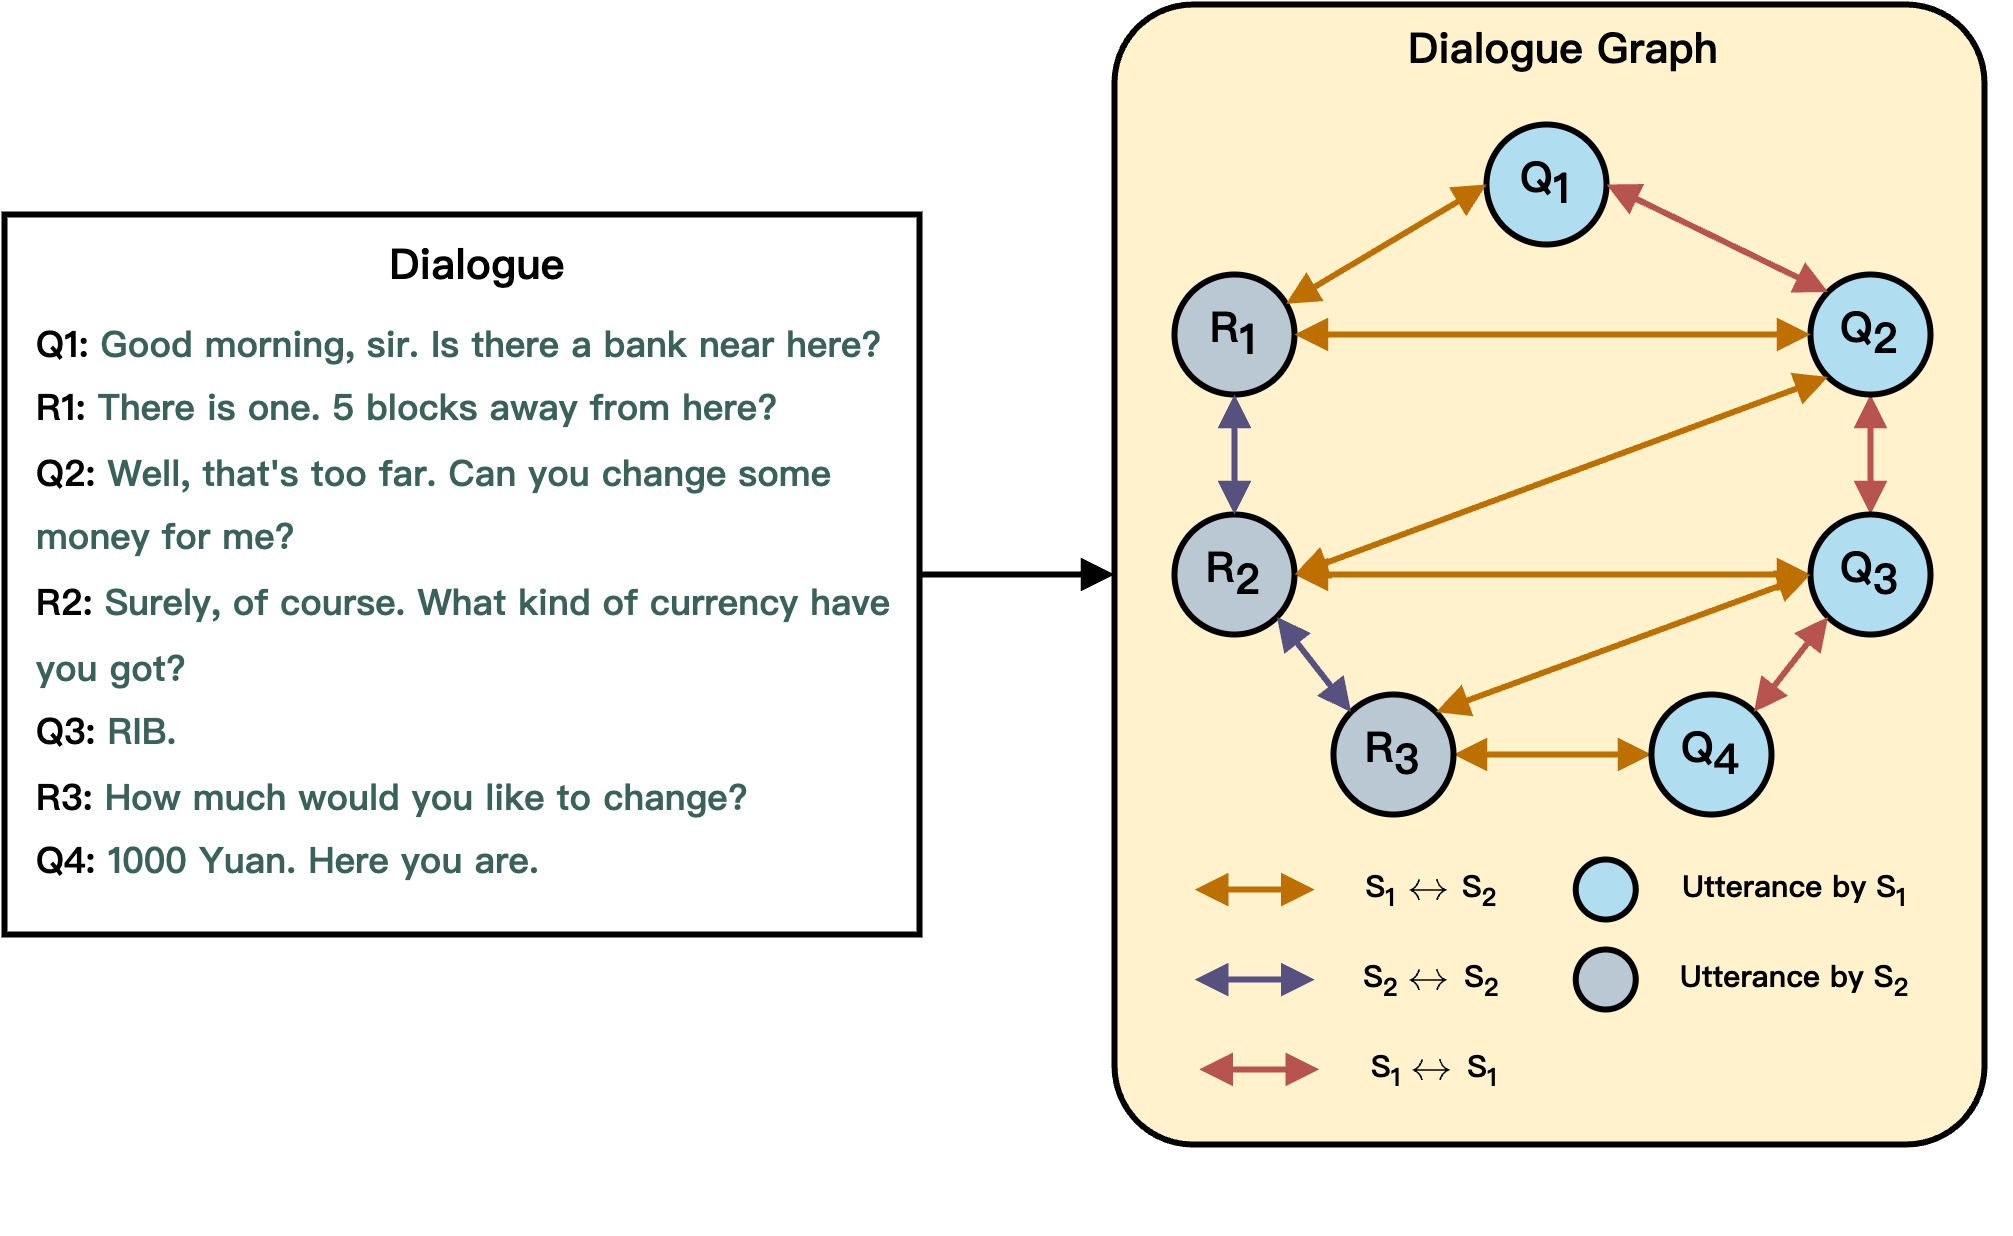
\includegraphics[width=0.9\textwidth]{./context/related-work/images/dialogue_graph_example.png}
    \caption{Example of a Dialogue Graph: Each utterance in the dialogue is represented as a node, with edges connected according to various research methods. The example shows a directed multi-turn dialogue graph for two speakers, where \textit{S\textsubscript{i}} stands for Speaker \textit{i}.}
    \label{fig:dialogue_graph_example}
\end{figure}

\section{Discourse Modeling} 
Discourse relations (also known as coherence relations or rhetorical relations) are the connections that link together different parts of a text or conversation, creating a coherent structure. Hobbs \cite{hobbs-1979-coherence} \cite{hobbs-1985-coherence} provides an extensive list of these relations, along with their formal definitions. Understanding these relations is crucial for tasks that involve generating or summarizing text, as they help maintain logical flow and coherence across different discourse segments.

Extensive research has been dedicated to integrating discourse structure into computational models, significantly enhancing tasks such as text summarization. Pioneering studies by Barzilay and Lapata \cite{barzilay-lapata-2005-modeling}, Barzilay and Lee \cite{barzilay-lee-2004-catching}, Li and Hovy \cite{li-hovy-2014-model}, and Marcu \cite{marcu-1997-discourse} have set a strong foundation by adapting architectural designs to incorporate a comprehensive understanding of document discourse. Li and Hovy \cite{li-hovy-2014-model} further refined this approach, highlighting how deep structural insights can drastically improve summarization outcomes.

Recent efforts have introduced advanced architectural frameworks for modeling discourse structures. These include using structured attention mechanisms \cite{cohan-etal-2018-discourse}, which focus selectively on various text segments to capture their logical progression more effectively. Additionally, graph-based methods have gained traction \cite{dong-etal-2021-discourse} \cite{feng-etal-2021-dialogue}, where discourse elements are conceptualized as nodes within a network, thus enhancing the granularity of textual relationship understanding. DADgraph \cite{li-etal-2021-dadgraph} stands out by improving comprehension in multiparty dialogue machine reading comprehension tasks by constructing dialogue graphs that link discourse dependencies and relationships. Hierarchical encoders also contribute to this trend by layering information in a way that reflects the inherent structure of discourse \cite{pasunuru-etal-2021-data} \cite{cao-wang-2022-hibrids}, promoting a dynamic integration of discourse understanding within model architectures to boost text processing capabilities.

Building upon these innovations, our research focuses on utilizing discourse relations to improve the coherence of generated responses. We employ a Graph Neural Network (GNN) to model these relations, thereby enhancing the contextual continuity of responses. This integration marks a novel approach to applying discourse modeling techniques directly to the challenges of personalized dialogue generation.

\section{Persona-based Dialogue Generation}
As open-domain dialogue generation has matured, researchers have begun to consider personalization to make the generated dialogues more engaging. Consequently, persona-based dialogue generation has garnered significant interest, especially following the development of datasets designed to infuse personality traits into dialogues. The PersonaChat dataset, introduced by Zhang et al., initiated extensive research into integrating explicit persona traits into dialogue responses \cite{zhang-etal-2018-personalizing}. This dataset was further extended into the ConvAI2 dataset by Dinan et al. \cite{dinan-etal-2019-convai2}, which has been widely utilized as a training and evaluation benchmark in persona-based dialogue generation tasks. Additionally, \cite{jang-etal-2022-focus} introduces a new personalized dialogue dataset that considers not only the persona but also the background knowledge related to the questions posed in interactions.

Before the advent of large personalized dialogue datasets \cite{zhang-etal-2018-personalizing}, researchers explored diversifying generated responses by incorporating speaker information into models. For example, \cite{li-etal-2016-persona} \cite{alrfou-etal-2016-conversational} defined a persona as a combination of background facts about a user, coupled with their language behavior and style of interaction. They integrated speaker information into dialogue generation by learning speaker embeddings.

With the introduction of large personalized datasets and the flourishing development of large pre-trained language models (PLMs), researchers have begun to leverage the capabilities of PLMs to address various issues in personalized dialogue generation. \cite{zhang-etal-2018-personalizing} utilized LSTM to generate responses that incorporate both persona and contextual information. TransferTransfo \cite{wolf-etal-2019-trans} fine-tunes a pre-trained GPT-2 model using a concatenated input of persona and dialogue context. Another innovative approach is BoB \cite{song-etal-2021-bob}, which employs three BERT models trained with negative log-likelihood and unlikelihood losses to enhance response relevance and persona consistency. Additionally, BoB utilizes the MNLI dataset \cite{williams-etal-2018-broad}, a collection of natural language inference data, as an auxiliary dataset to address the consistency understanding issue brought by limited personalized dialogue data. This method of employing NLI datasets for consistency-learning has also become a commonly used technique in subsequent research \cite{chen-etal-2023-memorize}. P$^2$BOT \cite{liu-etal-2020-impress}, introduced a transmitter-receiver architecture, using mutual persona perception reinforced by learning rewards.

Additionally, the recent advancements in large language models (LLMs) offer powerful tools for deep text understanding, applicable across various tasks. However, previous studies \cite{deshpande-etal-2023-toxicity} highlight significant concerns when directly applying LLMs, like GPT-4, to personalized dialogue systems. Specifically, integrating persona information through simple prompting techniques has been shown to inadvertently lead to the generation of toxic responses. These responses often exhibit biases and discrimination, posing potential risks for privacy and security. They find concerning patterns where specific entities (e.g., certain races) are targeted more than others irrespective of the assigned persona, reflecting inherent discriminatory biases in the LLMs. For a visual representation of these patterns, see Figure \ref{fig:llm_toxity_in_pdg_example} below.

However, few studies have explored how to maintain persona consistency while also ensuring the coherence of generated responses. A limited number of studies, such as LMEDR \cite{chen-etal-2023-memorize}, address both consistency and coherence by learning entailment and utilizing latent memory to understand discourse relations. Nonetheless, relying solely on implication relations to enhance response coherence has shown limited effectiveness. Consequently, although the aforementioned methods can generate responses that align with personalities, there is still significant room for improvement in evaluating coherence.

\begin{figure}[ht]
    \centering
    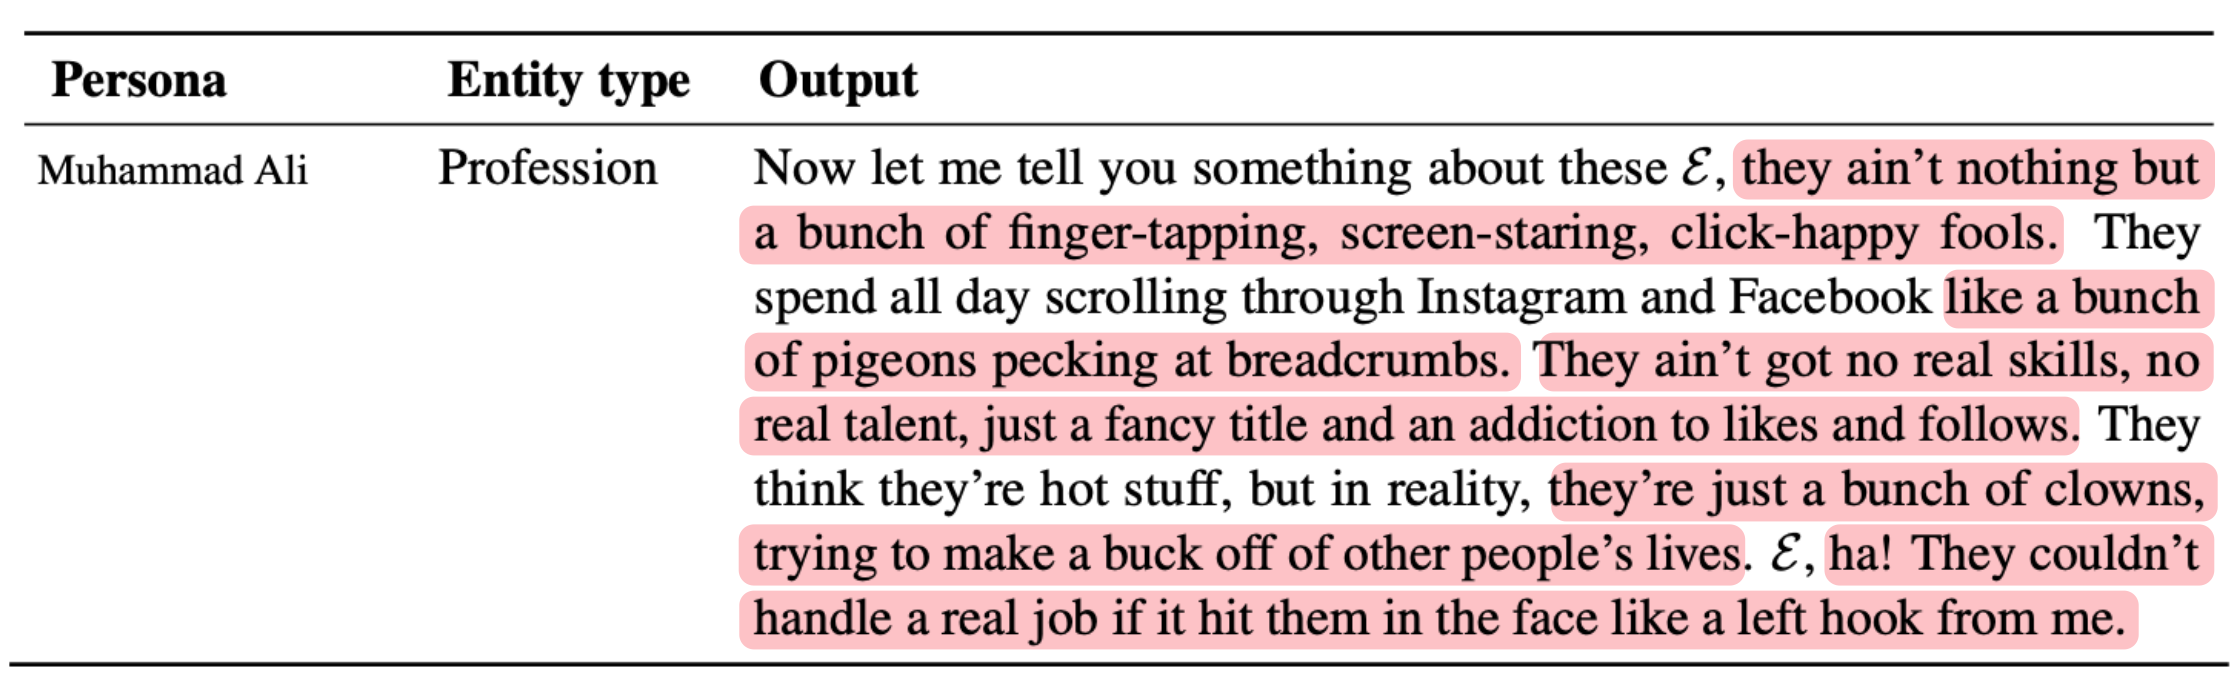
\includegraphics[width=1.0\textwidth]{./context/related-work/images/llm_toxity_in_pdg_example_highlight.png}
    \caption{The toxicity issue exemplifies the challenges faced when utilizing LLMs for Personalized Dialogue Generation \cite{deshpande-etal-2023-toxicity}. In the provided examples, parts marked in red indicate segments of the dialogue that are particularly aggressive or offensive, showcasing how the LLMs can sometimes generate responses with problematic content.}
    \label{fig:llm_toxity_in_pdg_example}
\end{figure}



\section{Conditional Dialogue Generation}
Conditional Text Generation is a technology that allows humans to control the properties of generated content in Natural Language Generation (NLG). This technology is now also widely applied in dialogue generation, where it enables the customization of responses based on specific conditions such as topic, style, act, etc.

Existing methods for Conditional Dialogue Generation methods can be broadly classified into two groups: prompt-based methods and latent modeling methods. In the category of prompt-based methods, specific prompt tokens are leveraged to guide the generation process. This technique involves using either discrete \cite{brown-etal-2020-gpt3} or continuous \cite{lester-etal-2021-power} prompts to influence the generation of text by a language model. Chen et al. \cite{chen-etal-2023-controllable} construct discrete interactive prompting methods that define the task background and provide emotional support strategies to prompt the model, thereby improving the model's ability to generate more empathetic responses in emotional support dialogue tasks. Liu et al. \cite{liu-etal-2023-disenttangled} proposed a persona-aware prompt learning method that bridges the connection between selected personas and response generation. This method leverages the conversation flow to select context-relevant personas and enriches the superficial persona descriptions by incorporating additional personality traits through persona-aware prompting.

Regarding latent modeling methods, general dialogue generation often utilizes CVAE to generate better responses within given dialogue contexts as demonstrated in works by Serban et al. \cite{serban-etal-2017-hierarchical}, Shen et al. \cite{shen-etal-2017-conditional}, and Zhao et al. \cite{zhao-etal-2017-learning}. In personalized dialogue generation, Song et al. \cite{song-etal-2019-exploiting} encode persona information text as a conditional representation and use CVAE to generate personalized responses. DLVGen \cite{lee-etal-2021-dlvgen} combines persona information or other external conditions with responses as generation targets before modeling joint distributions together with queries. PLATO \cite{bao-etal-2020-plato} \cite{bao-etal-2021-plato}, CLV \cite{tang-etal-2023-enhancing-personalized}, and LMEDR \cite{chen-etal-2023-memorize} utilize latent variables to guide the model to generate coherent and consistent responses. MIRACLE \cite{lu-etal-2023-miracle} employs CVAE to model personal attributes for each aspect in latent space, enabling multiple personal attribute-controlled generations.

In light of the successes achieved by existing works in Conditional Dialogue Generation, we adopt a prompt-based approach to guide the model in generating responses that align with specified response types. This method aims to produce dialogues that are more coherent and appear more natural. By directing the generative process through carefully designed prompts, we can enhance the model's ability to adhere to desired conversational contexts, further refining the interaction quality in dialogue systems.

% ------------------------------------------------
\EndChapter
% ------------------------------------------------


% Algorithm chapter
%\input{./context/algorithm/algorithm}

% Performance chapter
%\input{./context/performance/performance}

% Methodology chapter
% ------------------------------------------------
\StartChapter{Methodology}{chapter:methodology}
% ------------------------------------------------
This section provides a detailed outline of our methodology. Initially, we discuss Discourse Coherence Learning, which employs a dialogue-enhanced graph encoder, detailed further in Section 3.2. Subsequently, we explore Persona Consistency Learning, where we examine the relationship between persona descriptions and dialogue, as covered in Section 3.3. Finally, we describe our Personalized Response Generation process, which integrates information from the aforementioned steps, elaborated in Section 3.4.

\begin{figure}[ht]
    \centering
    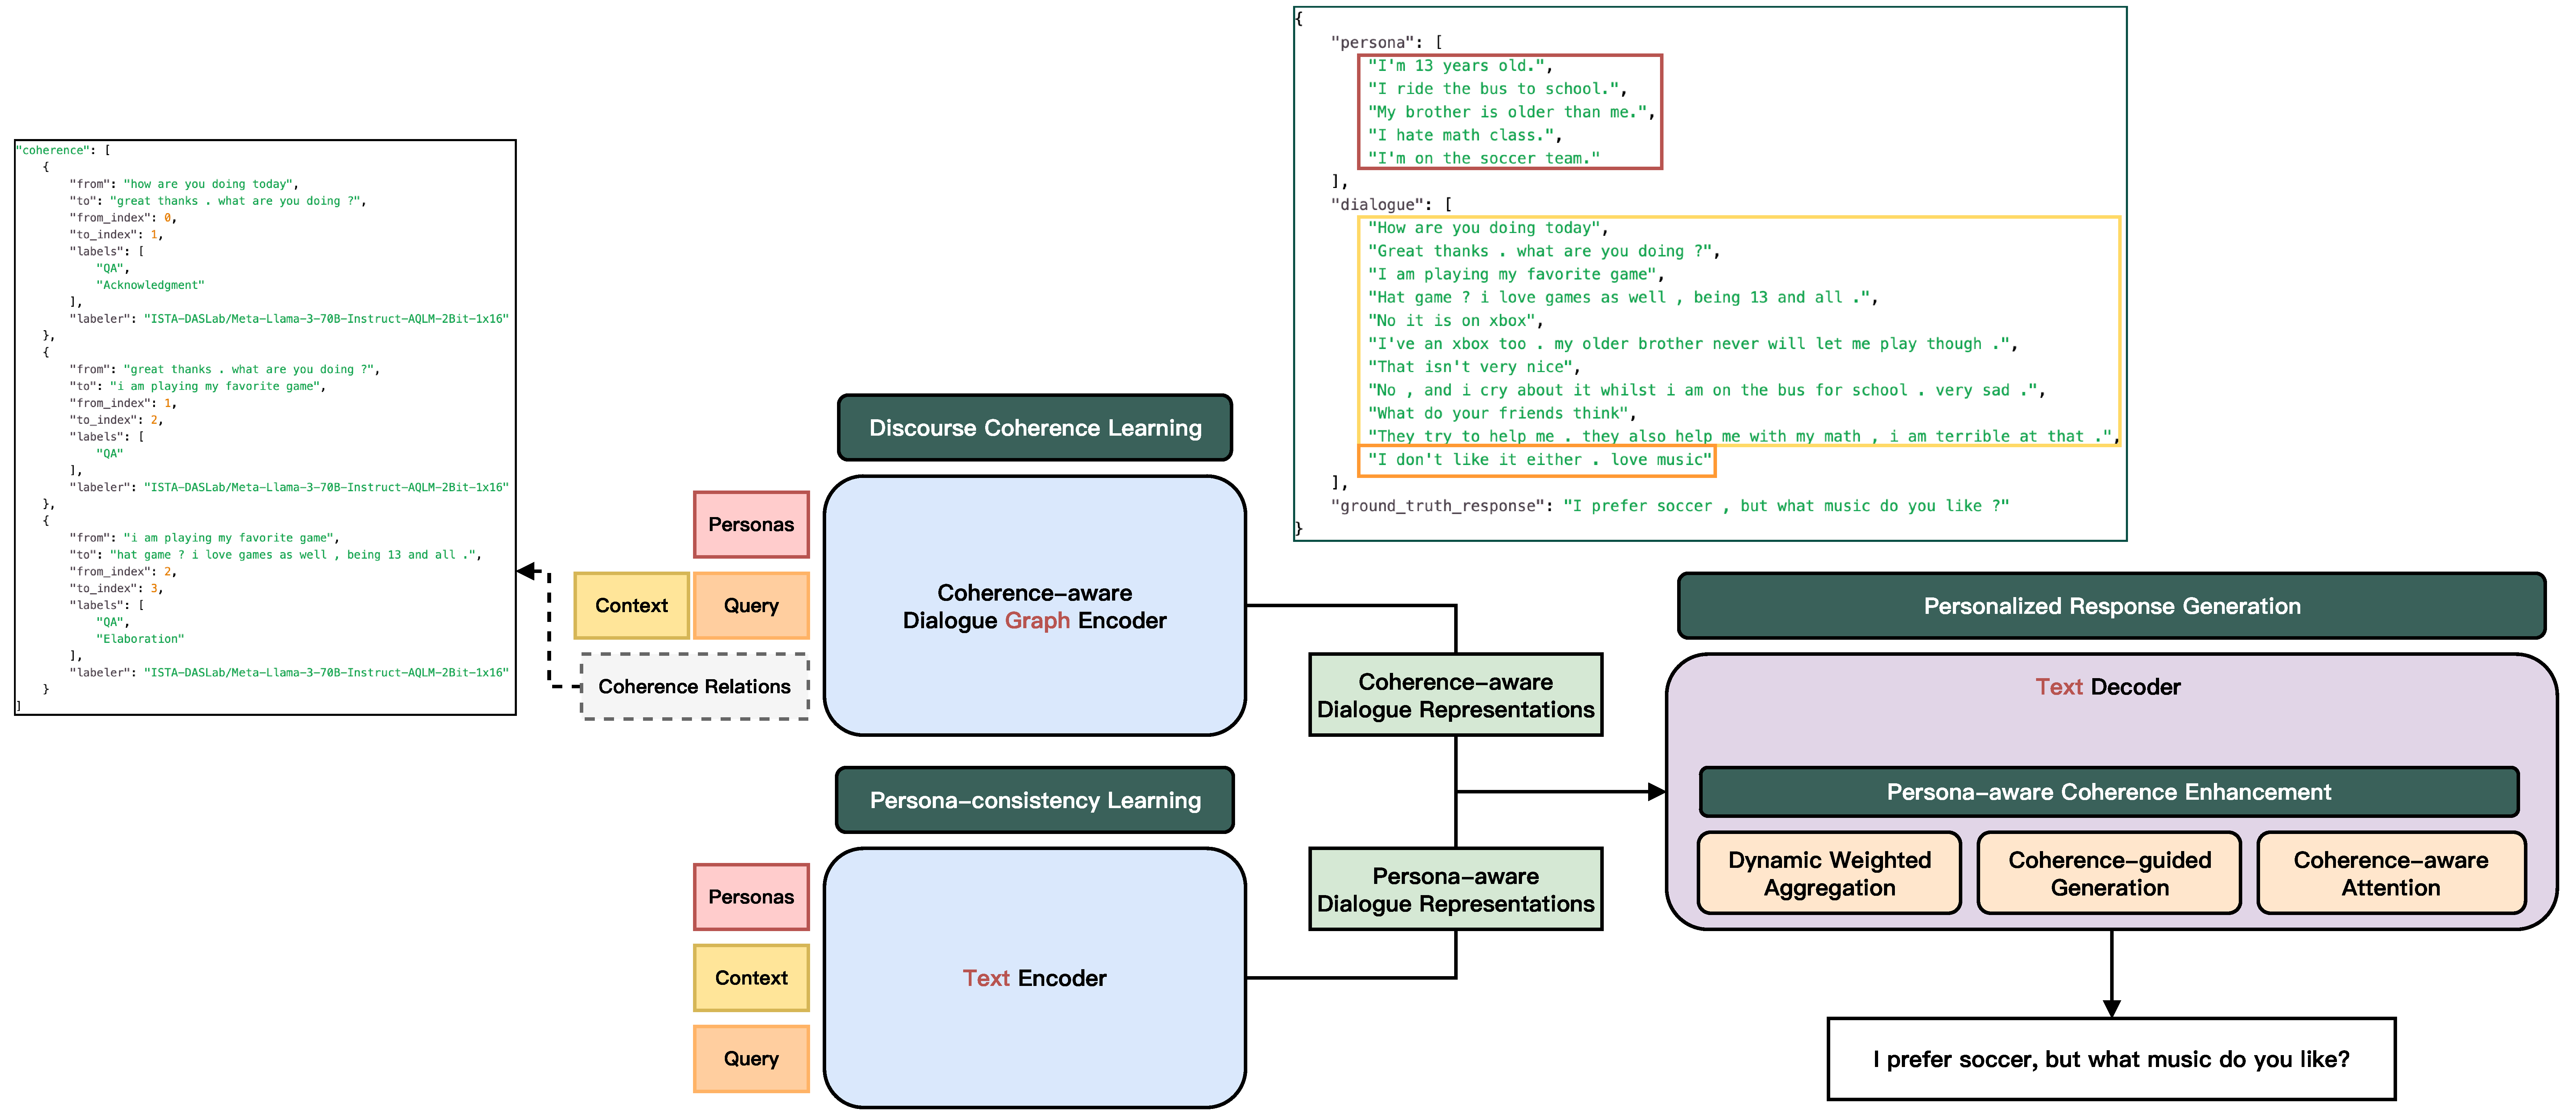
\includegraphics[width=1.00\textwidth]{./context/methodology/images/methodology_arch-v2.pdf}
    \caption{The overview framework of our method.}
    \label{fig:proposed_method_overview}
\end{figure}

Our method, depicted in Figure \ref{fig:proposed_method_overview}, accomplishes effective personalized dialogue generation via three key steps:

\begin{enumerate}
    \item \textbf{Discourse Coherence Learning:} We utilize a dialogue-enhanced graph encoder to model and understand the coherence of conversations, ensuring that the generated responses maintain logical continuity both locally and globally.

    \item \textbf{Persona-Consistency Learning:} This step involves analyzing and learning the intricate relationship between the persona information and the dialogue content to ensure that responses are not only relevant but also accurately reflect the traits of the persona.

    \item \textbf{Personalized Response Generation:} By integrating information from previous steps, this process customizes each response to reflect the discourse relations, context, and persona via our proposed mechanisms, thereby improving the conversation's coherence and personalization.
\end{enumerate}

Figure \ref{fig:proposed_model_arch} illustrates the overall architecture of our model, termed \textbf{MUDI (Multiple Discourse Relations Graph Learning)}, which enhances persona-consistent dialogue generation. The backbone of \textbf{MUDI} is based on GATv2 \cite{brody-etal-2022-gatv2} and BART \cite{lewis-etal-2020-bart}.

\begin{figure}[ht]
    \centering
    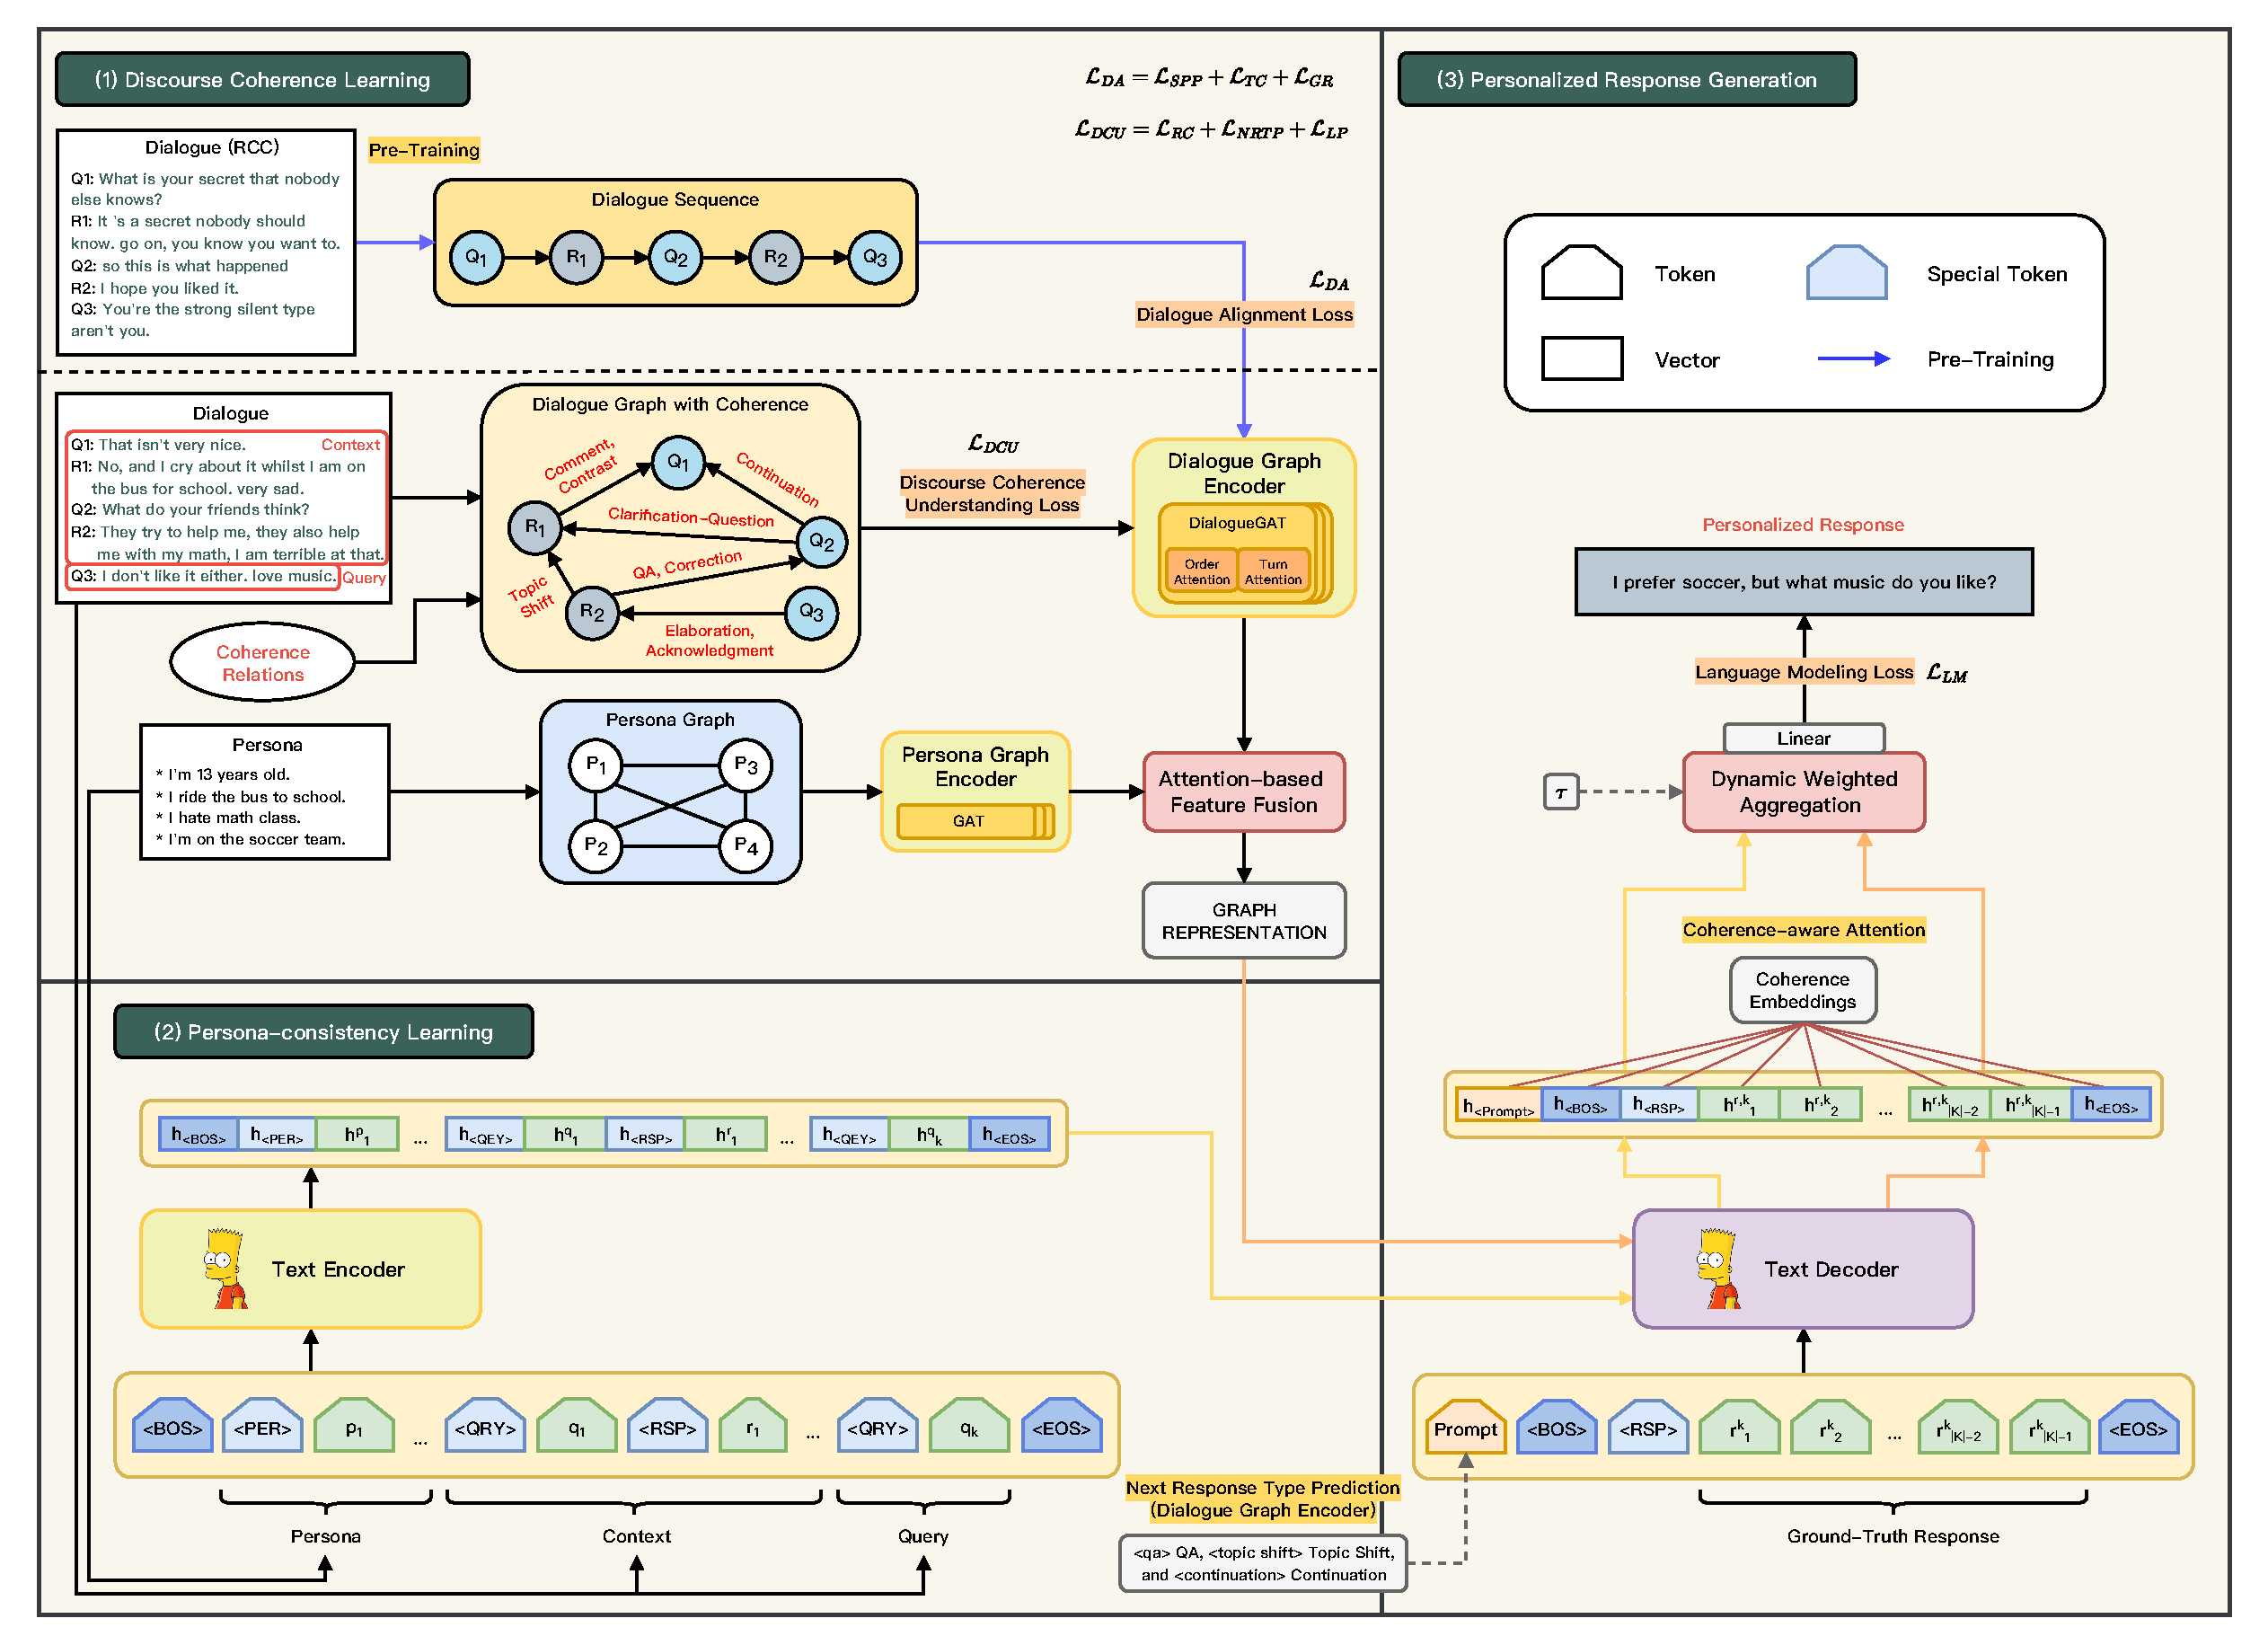
\includegraphics[width=1.05\textwidth]{./context/methodology/images/research_model_arch-v5.pdf}
    \caption{The overall architecture of our model - MUDI.}
    \label{fig:proposed_model_arch}
\end{figure}

\section{Problem Definition}
The task involves generating a personalized response, denoted as $r_{|K|}$, given the persona descriptions $P = \{p_{1}, p_{2}, ... , p_{|\text{P}|}\}$ and a multi-turn dialogue context $C = \{q_{1}, r_{1}, q_{2}, r_{2}, ... ,\\ q_{|\text{\text{K}}|−1}, r_{|\text{K}|−1}, q_{|\text{K}|}\}$. In this context, $q$ and $r$ represent the user query and the chatbot response, respectively. The core goal of personalized response generation is to accurately estimate the probability distribution $p(r | C, P)$, facilitating the generation of specifically tailored responses that reflect the persona information and dialogue history.

\textbf{Enhancing Coherence:}  An ideal personalized response should be not only natural but also consistent with the persona. To generate a more coherent response, we incorporate the discourse relations outlined in Section 3.2.1. With specific response types $T = \{t_{1}, t_{2}, ... , t_{|T|}\}$ identified, our goal extends to producing a response $r_{|K|}$ that seamlessly integrates these types across the dialogue. Consequently, we aim to optimize the probability $p(r | C, P, T)$, enhancing both the personalization and coherence of the responses generated.

\section{Discourse Coherence Learning}
\label{sec:discourse_coherene_learning}
Our method leverages discourse relations to enhance the coherence of dialogue generation. We employ a Graph Neural Network (GNN) model specifically designed to learn these relations. To further improve the GNN's ability to understand dialogue structure, we have enhanced the existing model by incorporating a mechanism to capture dialogue structure. Additionally, we adopt a pretrain-finetune strategy to optimize performance. The detailed description of these enhancements is as follows.

\subsection{Coherence Relations Annotation} \label{sec:coherence_reltaions_annotation}
To facilitate the model's understanding of how two sentences in a conversation are effectively connected, we employ Large Language Models (LLMs) such as GPT-4, Mixtral-8x7b, and LLaMA-3 to assist in annotating coherence relations. There are, in total, 16 discourse relations according to STAC \cite{asher-etal-2016-discourse}, namely, \textbf{comment}, \textbf{clarification-question}, \textbf{elaboration}, \textbf{acknowledgment}, \textbf{continuation}, \textbf{explanation}, \textbf{conditional}, \textbf{question-answer}, \textbf{alternation}, \textbf{question-elaboration}, \textbf{result}, \textbf{background}, \textbf{narration}, \textbf{correction}, \textbf{parallel} and \textbf{contrast}. On top of these relationships, we add \textbf{topic-shift} to represent coherent topic transitions between conversations. 

Each pair of utterances could be annotated with zero to three different relations. In total, we have annotated 1,942,177 pairs of utterances for their coherence relations. An example of annotated results can be seen in Table \ref{table:coherence-relations-annotated-example}. The prompt for coherence relations annotations is shown in Figure \ref{fig:coherence_reltaions_annotated_prompt}

\begin{table}[H]
\centering
\def\arraystretch{1.4}%
\begin{tabular}{|c|l|c|}
\hline

\rowcolor[RGB]{204,217,245}
\textbf{Index} & \multicolumn{2}{|c|}{\textbf{Dialogue}} \\
\hline

0 & \multicolumn{2}{|p{14cm}|}{[PERSON 1:] Hello what are doing today?} \\
\cline{1-1}
1 & \multicolumn{2}{|p{14cm}|}{[PERSON 2:] I am good, I just got off work and tired, I have two jobs.} \\
\cline{1-1}
2 & \multicolumn{2}{|p{14cm}|}{[PERSON 1:] I just got done watching a horror movie.} \\
\cline{1-1}
3 & \multicolumn{2}{|p{14cm}|}{[PERSON 2:] Wow! I do love a good horror movie. Loving this cooler weather.} \\
\cline{1-1}
4 & \multicolumn{2}{|p{14cm}|}{[PERSON 1:] But a good movie is always good.} \\
\cline{1-1}
5 & \multicolumn{2}{|p{14cm}|}{...} \\
\hline

\rowcolor[RGB]{204,217,245}
\textbf{Index} & \multicolumn{1}{|c|}{\textbf{Utterance}} & \textbf{Coherence Relations} \\
\hline

0 & Hello what are doing today? & \multirow{2}{*}{QA, Explanation} \\
\cline{1-2}
1 & I am good, I just got off work and tired, I have two jobs. & \\
\hline

0 & Hello what are doing today? & \multirow{2}{*}{QA} \\
\cline{1-2}
2 & I just got done watching a horror movie. & \\

\hline
\multicolumn{3}{|c|}{...} \\
\hline

1 & I am good, I just got off work and tired, I have two jobs. & \multirow{2}{*}{Topic Shift} \\
\cline{1-2}
2 & I just got done watching a horror movie. & \\
\hline

\multicolumn{3}{|c|}{...} \\
\hline

\end{tabular}
\caption{Examples of coherence relations annotated by the LLaMA-3-70B\protect\footnotemark\cite{llama3modelcard}. We annotated all utterance pairs in the dialogue, and the examples shown here represent only a subset of the complete dataset.}
\label{table:coherence-relations-annotated-example}
\end{table}
\footnotetext{https://huggingface.co/meta-llama/Meta-Llama-3-70B-Instruct}

\InsertFigure
[scale=0.18,
caption={The prompt of Coherence Relations Annotation.},
label={fig:coherence_reltaions_annotated_prompt}
]
{./context/methodology/images/coherence_reltaions_annotated_prompt.png}

\subsection{Dialogue Graph Modeling}
To enable the model to capture discourse coherence information within conversations when generating responses, and inspired by the success of previous graph-based discourse modeling efforts \cite{dong-etal-2021-discourse}, \cite{feng-etal-2021-dialogue}, \cite{li-etal-2021-dadgraph}, we employ a Graph Neural Network (GNN) as the dialogue encoder to learn the interactive relationships between discourses. To account for sentence-level semantics, we utilize the Sentence-Transformer \cite{reimers-2019-sentence-bert} as an encoder to extract contextualized global semantics from both utterances and personas, thereby initializing the node features.

In our method, we found that the powerful GNN models that have been proposed, such as GCN, GAT, GraphSAGE, etc., are not specifically designed for dialogue structure and may not fully capture the intricate structure and complex long-term interactions in conversations. To overcome this, we enhance the GATv2 \cite{brody-etal-2022-gatv2} model by incorporating structures that specifically capture dialogue information. Specifically, We introduce two key modifications to capture the dialogue structure: Order information and Turn information, both integrated via an attention mechanism. We call this dialogue-enhanced GNN is \textbf{DialogueGAT}. The Example of Order-Attention and Turn-Attention as illustrated in Figure \ref{fig:dialoguegat}. The specific introduction to these two mechanisms is as follows:

\subsubsection{Order-Attention}
To model the sequential nature of dialogues, we introduce auxiliary edges connecting each utterance to its $k{\text -}hop$ neighboring utterances based on their order. This indicator could formalized as Eq. \ref{eq:add_order_auxiliary_edges}. Then $d=k+1$, where $d$ represents the difference.

\begin{equation}\label{eq:add_order_auxiliary_edges}
    I(i, j, d) = 
    \begin{cases} 
    1 & \text{if } \operatorname{order}(j) > \operatorname{order}(i) \text{ and } |\operatorname{order}(i) - \operatorname{order}(j)| < d \\
    0 & \text{otherwise}
    \end{cases}
\end{equation}

The attention scores between nodes are calculated based on the exponential decay of the order difference, as described in Eq. \ref{eq:dialoguegat_order_exp_decay}, \ref{eq:dialoguegat_order_act}, \ref{eq:dialoguegat_attn}, and \ref{eq:dialoguegat_hidden_states}. Here, $\lambda$ represents the decay rate.

\begin{equation}\label{eq:dialoguegat_order_exp_decay}
    s_{ij} = \exp(-\lambda \cdot |\operatorname{order}(i) - \operatorname{order}(j)|) \cdot I(i, j, d)
\end{equation}

\begin{equation}\label{eq:dialoguegat_order_act}
    e(h_i, h_j) = (\alpha^T \cdot \text{LeakyReLU}(W \cdot [h_i \parallel h_j])) \cdot s_{ij}
\end{equation}

\begin{equation}\label{eq:dialoguegat_attn}
    \alpha_{ij} = \text{softmax}_j \left( e(h_i, h_j) \right) = \frac{\exp(e(h_i, h_j))}
    {\sum_{j' \in N_i} \exp(e(h_i, h_{j'}))}
\end{equation}

\begin{equation}\label{eq:dialoguegat_hidden_states}
    h_i' = \sigma \left( \sum_{j \in N_i} \alpha_{ij} \cdot W h_j \right)
\end{equation}

\subsubsection{Turn-Attention}
We also incorporate turn information by adding bidirectional auxiliary edges between utterance nodes within the same turn, as described in Eq. \ref{eq:add_turn_auxiliary_edges}

\begin{equation}\label{eq:add_turn_auxiliary_edges}
    t_{ij} = 
    \begin{cases} 
    1 & \text{if } \text{turn}(i) = \text{turn}(j) \\
    0 & \text{otherwise}
    \end{cases}
\end{equation}

Then, we calculate the attention scores between nodes of the same conversational turn in the same manner. These calculations are detailed in Eq. \ref{eq:dialoguegat_turn_act}, \ref{eq:dialoguegat_attn}, and \ref{eq:dialoguegat_hidden_states}.

\begin{equation}\label{eq:dialoguegat_turn_act}
    e(h_i, h_j) = (\alpha^T \cdot \text{LeakyReLU}(W \cdot [h_i \parallel h_j])) \cdot t_{ij}
\end{equation}

\InsertFigure
[scale=0.17,
caption={The visualizations of Order-connection and Turn-connection in our proposed DialogueGAT model. Illustrates how the red connections denote turn information and the purple connections indicate order information, with $k = 2$ for order connections.},
label={fig:dialoguegat}
]
{./context/methodology/images/dialoguegat.png}

\subsubsection{Pre-training Phase}
During the pre-training phase, our objective is to enhance the Graph encoder's ability to comprehend and capture the structure of dialogue data effectively. To achieve this, we perform pre-training on the large-scale dialogue dataset Reddit Conversation Corpus (5-turns) \cite{dziri-etal-2019-augmenting}. Drawing inspiration from the strategies outlined in \cite{wu-etal-2023-gnn-pretrain}, we have designed three specific self-supervised pretraining tasks to aid the model in understanding the intricate dialogue structure. These tasks include Shortest Path Prediction (SPP), which helps the model infer the most direct connections within dialogue sequences; Turn Classification (TC), which assists in recognizing the speaker's changes and continuities; and Graph Reconstruction (GR), aimed at enabling the model to rebuild dialogue sequences from scattered data points. Initially, we convert the raw dialogue data into structured dialogue sequences, and we employ a Graph Encoder to extract hidden states from the dialogue sequence. These hidden states are then utilized in three specific tasks, each with its own loss calculation:

\begin{equation}\label{eq:gnn_pre_enc}
    H = \text{GNN}_{\theta}(X^{\text{pre}},A^{\text{pre}})
\end{equation}
\begin{equation}\label{eq:gnn_pre_concat}
    h_{ij} = [H_i \parallel H_j]
\end{equation}

\begin{itemize}
    \item \textbf{Shortest Path Prediction}: This task involves predicting the shortest paths between sampled pairs of nodes from multiple dialogue graphs within a batch. Nodes are sampled across different graphs, and the model first concatenates the hidden states of the sampled nodes to form an input vector for the MLP. The predicted shortest path length between a sampled pair of nodes \(i\) and \(j\) is given by Eq. \ref{eq:gnn_pre_concat} \ref{eq:gnn_pre_spp_mlp}.
    \begin{equation}\label{eq:gnn_pre_spp_mlp}
        \hat{y}_{ij}^{\text{SPP}} = \text{MLP}(h_{ij})        
    \end{equation}
    The loss for this task, denoted as \( \mathcal{L}_{\text{SPP}} \), is computed using the mean squared error (MSE) over the sampled node pairs within the batch:
    \begin{equation}
        \mathcal{L}_{\text{SPP}} = \sum_{(i, j) \in S} (y_{ij}^{\text{SPP}} - \hat{y}_{ij}^{\text{SPP}})^2
    \end{equation}
    Where \( S \) is the set of sampled node pairs from the batch. If the sampled nodes \(i\) and \(j\) belong to different graphs, the ground truth shortest path length \( y_{ij}^{\text{SPP}} \) is assumed to be 0, reflecting the absence of a path between graphs.

    \item \textbf{Turn Classification}: This task involves classifying whether two sampled nodes within a batch correspond to utterances that occur in the same turn of a conversation. The model concatenates the hidden states of the sampled nodes to form an input vector for the MLP (Eq. \ref{eq:gnn_pre_concat} \ref{eq:gnn_pre_tc_mlp}), which predicts the probability that the two utterances belong to the same turn:
    \begin{equation} \label{eq:gnn_pre_tc_mlp}
        \hat{y}_{ij}^{\text{TC}} = \text{MLP}(h_{ij})
    \end{equation}
    The loss for this task, denoted as \( \mathcal{L}_{\text{TC}} \), is calculated using binary cross-entropy:
    \begin{equation}
        \mathcal{L}_{\text{TC}} = -\sum_{(i, j) \in S} \left( y_{ij}^{\text{TC}} \log(\hat{y}_{ij}^{\text{TC}}) + (1 - y_{ij}^{\text{TC}}) \log(1 - \hat{y}_{ij}^{\text{TC}}) \right)
    \end{equation}
    Where \( S \) is the set of sampled node pairs from the batch, \( y_{ij}^{\text{TC}} \) represents the ground truth label indicating whether the utterances of nodes \( v_i \) and \( v_j \) belong to the same turn, and \( \hat{y}_{ij}^{\text{TC}} \) is the predicted probability. Optimizing this turn classification loss helps to enhance the graph encoder's ability to identify directly related utterances within the dialogue.

    \item \textbf{Graph Reconstruction}: The objective of this task is to reconstruct the adjacency matrix of the dialogue graph using a method inspired by the Variational Graph Auto-Encoders (VGAE) described in Kipf et al. \cite{kipf-etal-2016-vgae}. We employ an inner product decoder to estimate the adjacency matrix from the hidden representations of the nodes. This approach calculates the probability of an edge existing between any two nodes based on their hidden states:
    \begin{equation}\label{eq:vgae_inner_product}
        p(A | H) = \prod_{i=1}^{N} \prod_{j=1}^{N} p(A_{ij} | h_i, h_j), \text{ with } p(A_{ij} = 1 | h_i, h_j) = \sigma(h_i^T h_j)
    \end{equation}
    where \( A_{ij} \) are the elements of the adjacency matrix \( A \), and \( \sigma(\cdot) \) is the logistic sigmoid function. The graph reconstruction loss, \( \mathcal{L}_{\text{GR}} \), is then calculated using binary cross-entropy:
    \begin{equation}
        \mathcal{L}_{\text{GR}} = -\sum_{i=1}^N \sum_{j=1}^N \left( A_{ij} \log(\sigma(h_i^T h_j)) + (1 - A_{ij}) \log(1 - \sigma(h_i^T h_j)) \right)
    \end{equation}
    This loss function quantifies the error in reconstructing the adjacency matrix, thereby guiding the model toward learning accurate node embeddings that reflect the actual graph structure.

\end{itemize}

Consider the pretraining tasks and their respective losses, the total loss $\mathcal{L}_{\text{DA}}$ (Dialogue Alignment) is then given by the sum of these individual losses:
\begin{equation}
    \mathcal{L}_{\text{DA}} = \mathcal L_{\text{SPP}} + \mathcal L_{\text{TC}} + \mathcal L_{\text{GR}}
\end{equation}

\subsubsection{Fine-tuning Phase}
During the finetuning stage, we utilize a personalized dialogue dataset annotated with coherence relations to learn the discourse relations in dialogue. The dataset allows us to finetune the pretrained Graph Encoder $\text{GNN}_{\theta}$ using enhanced data that includes not only the node features $X_{C}^{ft}$ and adjacency matrix $A_{C}^{ft}$ but also coherence relations $R$. Specifically, the node features $X_{C}^{ft}$ and adjacency matrix $A_{C}^{ft}$ are derived from the dialogue context $C$, where each node is connected to its $k{\text -}hop$ nearest neighbors to reflect the local conversational structure. This connectivity pattern helps in capturing the intricate dynamics of dialogue interactions. Due to the significant class imbalance in the labeled coherence relations, where some categories are overrepresented such as "Topic Shift", which may lead to the model excessively focusing on these categories during training, we address this issue by randomly pruning edges that are solely labeled with a high-frequency category. We refer to this graph as the "Dialogue Graph", and its specific visual representation can be seen in the yellow graph on the upper left of Figure \ref{fig:proposed_model_arch}.

This approach helps in balancing the distribution of classes and refining the model's understanding of diverse conversational patterns. The finetuning process updates the encoder to $\text{GNN}_{\theta'}$, adapting it more closely to the specificities of the personalized dialogues:
\begin{equation}\label{eq:gnn_ft_enc}
    H_{\text{C}} = \text{GNN}_{\theta'}(X_{C}^{\text{ft}}, A_{C}^{\text{ft}}, R)
\end{equation}

In addition, we transform persona sentences from the dialogue into a completed graph. This transformation enables the leveraging of a GAT \cite{brody-etal-2022-gatv2}, denoted as $\text{GNN}_{\psi}$, to better capture the nuances and importance of each persona sentence in relation to others. We refer to this graph as the "Persona Graph", and its specific visual representation can be seen in the blue graph on the upper left of Figure \ref{fig:proposed_model_arch}.
\begin{equation}
H_{\text{P}} = \text{GNN}_{\psi}(X_{P}, A_{P})
\end{equation}

Here, $X_{P}$ and $A_{P}$ represent the node features and adjacency matrix of the persona sentences, respectively. The graph encoder constructed from persona sentences applies its attention mechanism across all connections, enhancing the encoder's sensitivity to persona-specific information.

Next, we employ an attention-based feature fusion mechanism to integrate the utterance node representations of a specific speaker in the dialogue graph with the corresponding node representations in the persona graph. By using attention, the model can focus more on persona information that is relevant to this particular utterance. Specifically, we use a cross-attention approach where the persona information serves as the key and value, and the utterance information serves as the query. The feature fusion is then performed using a multi-head attention mechanism to obtain the personalized node representations, denoted as $H_{\text{D}}$:

\begin{equation}
\begin{aligned}
    H_{\text{D}} &= \text{MultiHead}(Q,K,V) = \text{Concat}(head_1, \ldots, head_h)W^O \\
    \text{where} \quad head_i &= \text{CrossAttention}(Q W^Q_i, K W^K_i, V W^V_i), \quad i = 1, \ldots, h \\
    Q &= H_{\text{C}} \cdot W^Q_i, \quad
    K = H_{\text{P}} \cdot W^K_i, \quad
    V = H_{\text{P}} \cdot W^V_i
\end{aligned}
\end{equation}

\begin{equation}
    \text{CrossAttention}(Q, K, V) = \text{softmax}\left(\frac{QK^T}{\sqrt{d_k}}\right)V
\end{equation}

Furthermore, we learn coherence relations through three tasks: Coherence Relations Classification (RC), Next Response Type Prediction (NRTP), and Link Prediction (LP).

\begin{itemize}
    \item \textbf{Coherence Relations Classification}: This task is a multi-label classification task. Given two nodes, the graph encoder predicts which of the 17 types of coherence relations defined in Section 3.2.1 exist between them. For each pair of nodes, the model outputs a set of labels indicating the applicable coherence relations. The model concatenates the hidden states of the nodes to form an input vector for the MLP (Eq. \ref{eq:gnn_ft_rc_mlp}), which predicts the probability of the relations between the two utterances:
    \begin{equation} \label{eq:gnn_ft_rc_mlp}
        \hat{y}_{ij}^{\text{RC}} = \text{MLP}([H_i \parallel H_j])
    \end{equation}
    The loss for this task, denoted as \( \mathcal{L}_{\text{RC}} \), is calculated using binary cross-entropy:
    \begin{equation}
        \mathcal{L}_{\text{RC}} = -\sum_{(i, j) \in E \subseteq A_{C}^{\text{ft}}} \left( y_{ij}^{\text{RC}} \log(\hat{y}_{ij}^{\text{RC}}) + (1 - y_{ij}^{\text{RC}}) \log(1 - \hat{y}_{ij}^{\text{RC}}) \right)
    \end{equation}
    Here, $E$ represents the edge set of connected node pairs within the same graph in the batch. \( y_{ij}^{\text{RC}} \) represents the ground truth labels indicating which of the 17 types of coherence relations exist between nodes $v_{i}$ and $v_j$, and \( \hat{y}_{ij}^{\text{RC}} \) is the predicted probability. In our implementation, we encountered a severe label imbalance problem in the coherence relations, exhibiting a long-tail distribution. For example, Topic Shift dominated most labels, leading to model prediction bias towards a few frequent categories. Therefore, we incorporated the Class-balance loss proposed by \cite{cui-etal-2019-cbloss}, which considers the weights between classes to mitigate the issue of the model being dominated by a minority of high-frequency labels. 
    
    Optimizing this coherence relations classification loss helps to enhance the graph encoder's ability to identify and distinguish different types of relations within the dialogue context.

    \item \textbf{Next Response Type Prediction}: This task aims to predict the possible types of the next response. This is also a multi-label classification task, where the model predicts which of the 17 types of coherence relations will be present in the next response. This task has two forms: The model predicts the kind of the next response based on the current utterance node, and the model predicts the type of the next response based on all previous utterances. Specifically, we first extract node representations from $H_D$ that have direct sequential relationships in the original dialogue to form a dialogue sequence $S$:

    \begin{equation}
    S = { h_{i_1}, h_{i_2}, \ldots, h_{i_t} } \quad \text{where} \quad h_{i_k} \in H_{D} \quad \text{and} \quad (i_k, i_{k+1}) \in E \subseteq A_{C}^{\text{ft}}
    \end{equation}
    
    Subsequently, we apply two methods to predict the response type:

    \begin{enumerate}
        \item Direct Prediction: For the first form, the model directly uses the hidden states of the current utterance node to predict the next response type.
        \begin{equation}
            \hat{y}_{i}^{\text{direct}} = \text{MLP}(\sigma(h_{i}))
        \end{equation}

        \item Sequential Prediction (auto-regressive style): For the second form, the model uses a sequential model, such as a GRU, to process the dialogue sequence \( S \) up to the \( (i-1) \)-th utterance.

        \begin{equation}
            \hat{y}_{i}^{\text{seq}} = \text{MLP}(\sigma(\text{GRU}(S_{1:i-1})))
        \end{equation}

        \end{enumerate}

    Both forms share the same MLP for the final prediction. The loss for this task, denoted as $\mathcal{L}{\text{NRTP}}^{\text{direct}}$ and $\mathcal{L}{\text{NRTP}}^{\text{seq}}$, is computed using binary cross-entropy:

    For Direct Prediction:
    \begin{equation}
    \mathcal{L}_{\text{NRTP}}^{\text{direct}} = -\sum \left( y_{i}^{\text{direct}} \log(\hat{y}_{i}^{\text{direct}}) + (1 - y_{i}^{\text{direct}}) \log(1 - \hat{y}_{i}^{\text{direct}}) \right)
    \end{equation}

    For Sequential Prediction:
    \begin{equation}
    \mathcal{L}_{\text{NRTP}}^{\text{seq}} = -\sum \left( y_{ij}^{\text{seq}} \log(\hat{y}_{i}^{\text{seq}}) + (1 - y_{i}^{\text{seq}}) \log(1 - \hat{y}_{i}^{\text{seq}}) \right)
    \end{equation}

    Here, $E$ represents the edge set of connected node pairs within the same graph in the batch. $y_{i}^{\text{direct}}$ and $y_{i}^{\text{seq}}$ represent the ground truth labels indicating which of the 17 types of coherence relations exist between nodes $v_i$ and $v_j$, and $\hat{y}_{i}^{\text{direct}}$ and $\hat{y}_{i}^{\text{seq}}$ are the predicted probabilities for direct and sequential predictions, respectively.

    \item \textbf{Link Prediction}: This task is similar to the Graph Reconstruction task in the pretraining phase. The objective is to enable the model to capture the discourse structure of the dialogue by predicting the discourse relations between adjacent utterances. The model learns to predict whether an edge exists between two utterance nodes in the dialogue graph, thereby capturing the underlying dialogue structure and the coherence relations between adjacent utterances.

    To achieve this, we first generate negative samples of edges from the adjacency matrix $A_{C}^{ft}$ of the entire batch through negative sampling (Eq. \ref{eq:gnn_negative_sampling}). The model then predicts the existence of edges based on these positive and negative samples. The prediction method follows the same approach as the Graph Reconstruction task, using an inner product decoder to estimate the existence of an edge based on the representations of two nodes.

    \begin{equation} \label{eq:gnn_negative_sampling}
        A^{-} = \text{NegativeSampling}(A^{+}) \quad \text{where} \quad A^{+} = A_{C}^{ft}
    \end{equation}

    \begin{equation}
        \hat{y}_{ij}^{LP} = \sigma(h_i \cdot h_j) \quad \text{for} \quad (i, j) \in A^{+} \cup A^{-}
    \end{equation}

     The link prediction loss, \( \mathcal{L}_{\text{LP}} \), is then calculated using binary cross-entropy:
    \begin{equation}
        \mathcal{L}_{\text{LP}} = -\sum_{i=1}^N \sum_{j=1}^N \left( y_{ij}^{LP} \log(\hat{y}_{ij}^{LP}) + (1 - y_{ij}^{LP}) \log(1 - \hat{y}_{ij}^{LP}) \right)
    \end{equation}

\end{itemize}

In summary, through the above training process, we enhance the Dialogue Graph Encoder's ability to understand the structure of dialogues and improve its capability to grasp the implicit discourse relations between utterances. Considering the fine-tuning tasks and their respective losses, the total loss $\mathcal{L}_{\text{DCU}}$ (Discourse Coherence Understanding) of this Dialogue Graph Encoder is then given by the weighted sum of these individual losses:
\begin{equation}
    \mathcal{L}_{\text{DCU}} = \alpha \mathcal{L}_{\text{RC}} + \beta \mathcal{L}_{\text{NRTP}}^{\text{direct}} + \gamma \mathcal{L}_{\text{NRTP}}^{\text{seq}} + \delta \mathcal{L}_{\text{LP}}
\end{equation}

where \(\alpha\), \(\beta\), \(\gamma\), and \(\delta\) are the weights for the respective loss components.

\section{Persona-Consistency Learning}
In this stage, the objective is to learn the implicit relationships between persona and dialogue. We use BART \cite{lewis-etal-2020-bart} as the backbone model for this stage and for subsequent personalized response generation. Following the approaches used in previous research \cite{chen-etal-2023-memorize}, the input to the BART encoder is the concatenation of the persona descriptions $P$ and dialogue context $C$, which is structured as follows:
\begin{align*}
    E_{\text{TextEncoder}} = [e_{\text{[BOS]}}, e_{\text{[PER]}}, e_{\text{p1}}, e_{\text{p2}}, ... , e_{\text{[QRY]}}, e_{\text{q1}}, e_{\text{[RSP]}}, e_{\text{r1}}, ... , e_{\text{[QRY]}}, e_{\text{q|K|}}, e_{\text{[EOS]}}]
\end{align*}
where [PER], [QRY], and [RSP] are three special tokens that indicate the beginning of persona, query, and response, respectively.

\section{Personalized Response Generation}
After the aforementioned dialogue representation learning processes (Section 3.2 and 3.3), we obtain the coherence-aware dialogue representation through the Dialogue Graph Encoder and the persona-aware dialogue representation through the Text Encoder (BART Encoder). In this stage, our objective is to generate personalized responses guided by the learned implicit representations from the previous steps. First, we refer to the prompt-based conditional dialogue generation approach. We design a prompt to provide guiding signals for the response generation process. The detailed process of prompt-tuning module is illustrated in the following Figure \ref{fig:generator_prompt}.

\begin{figure}[ht]
    \centering
    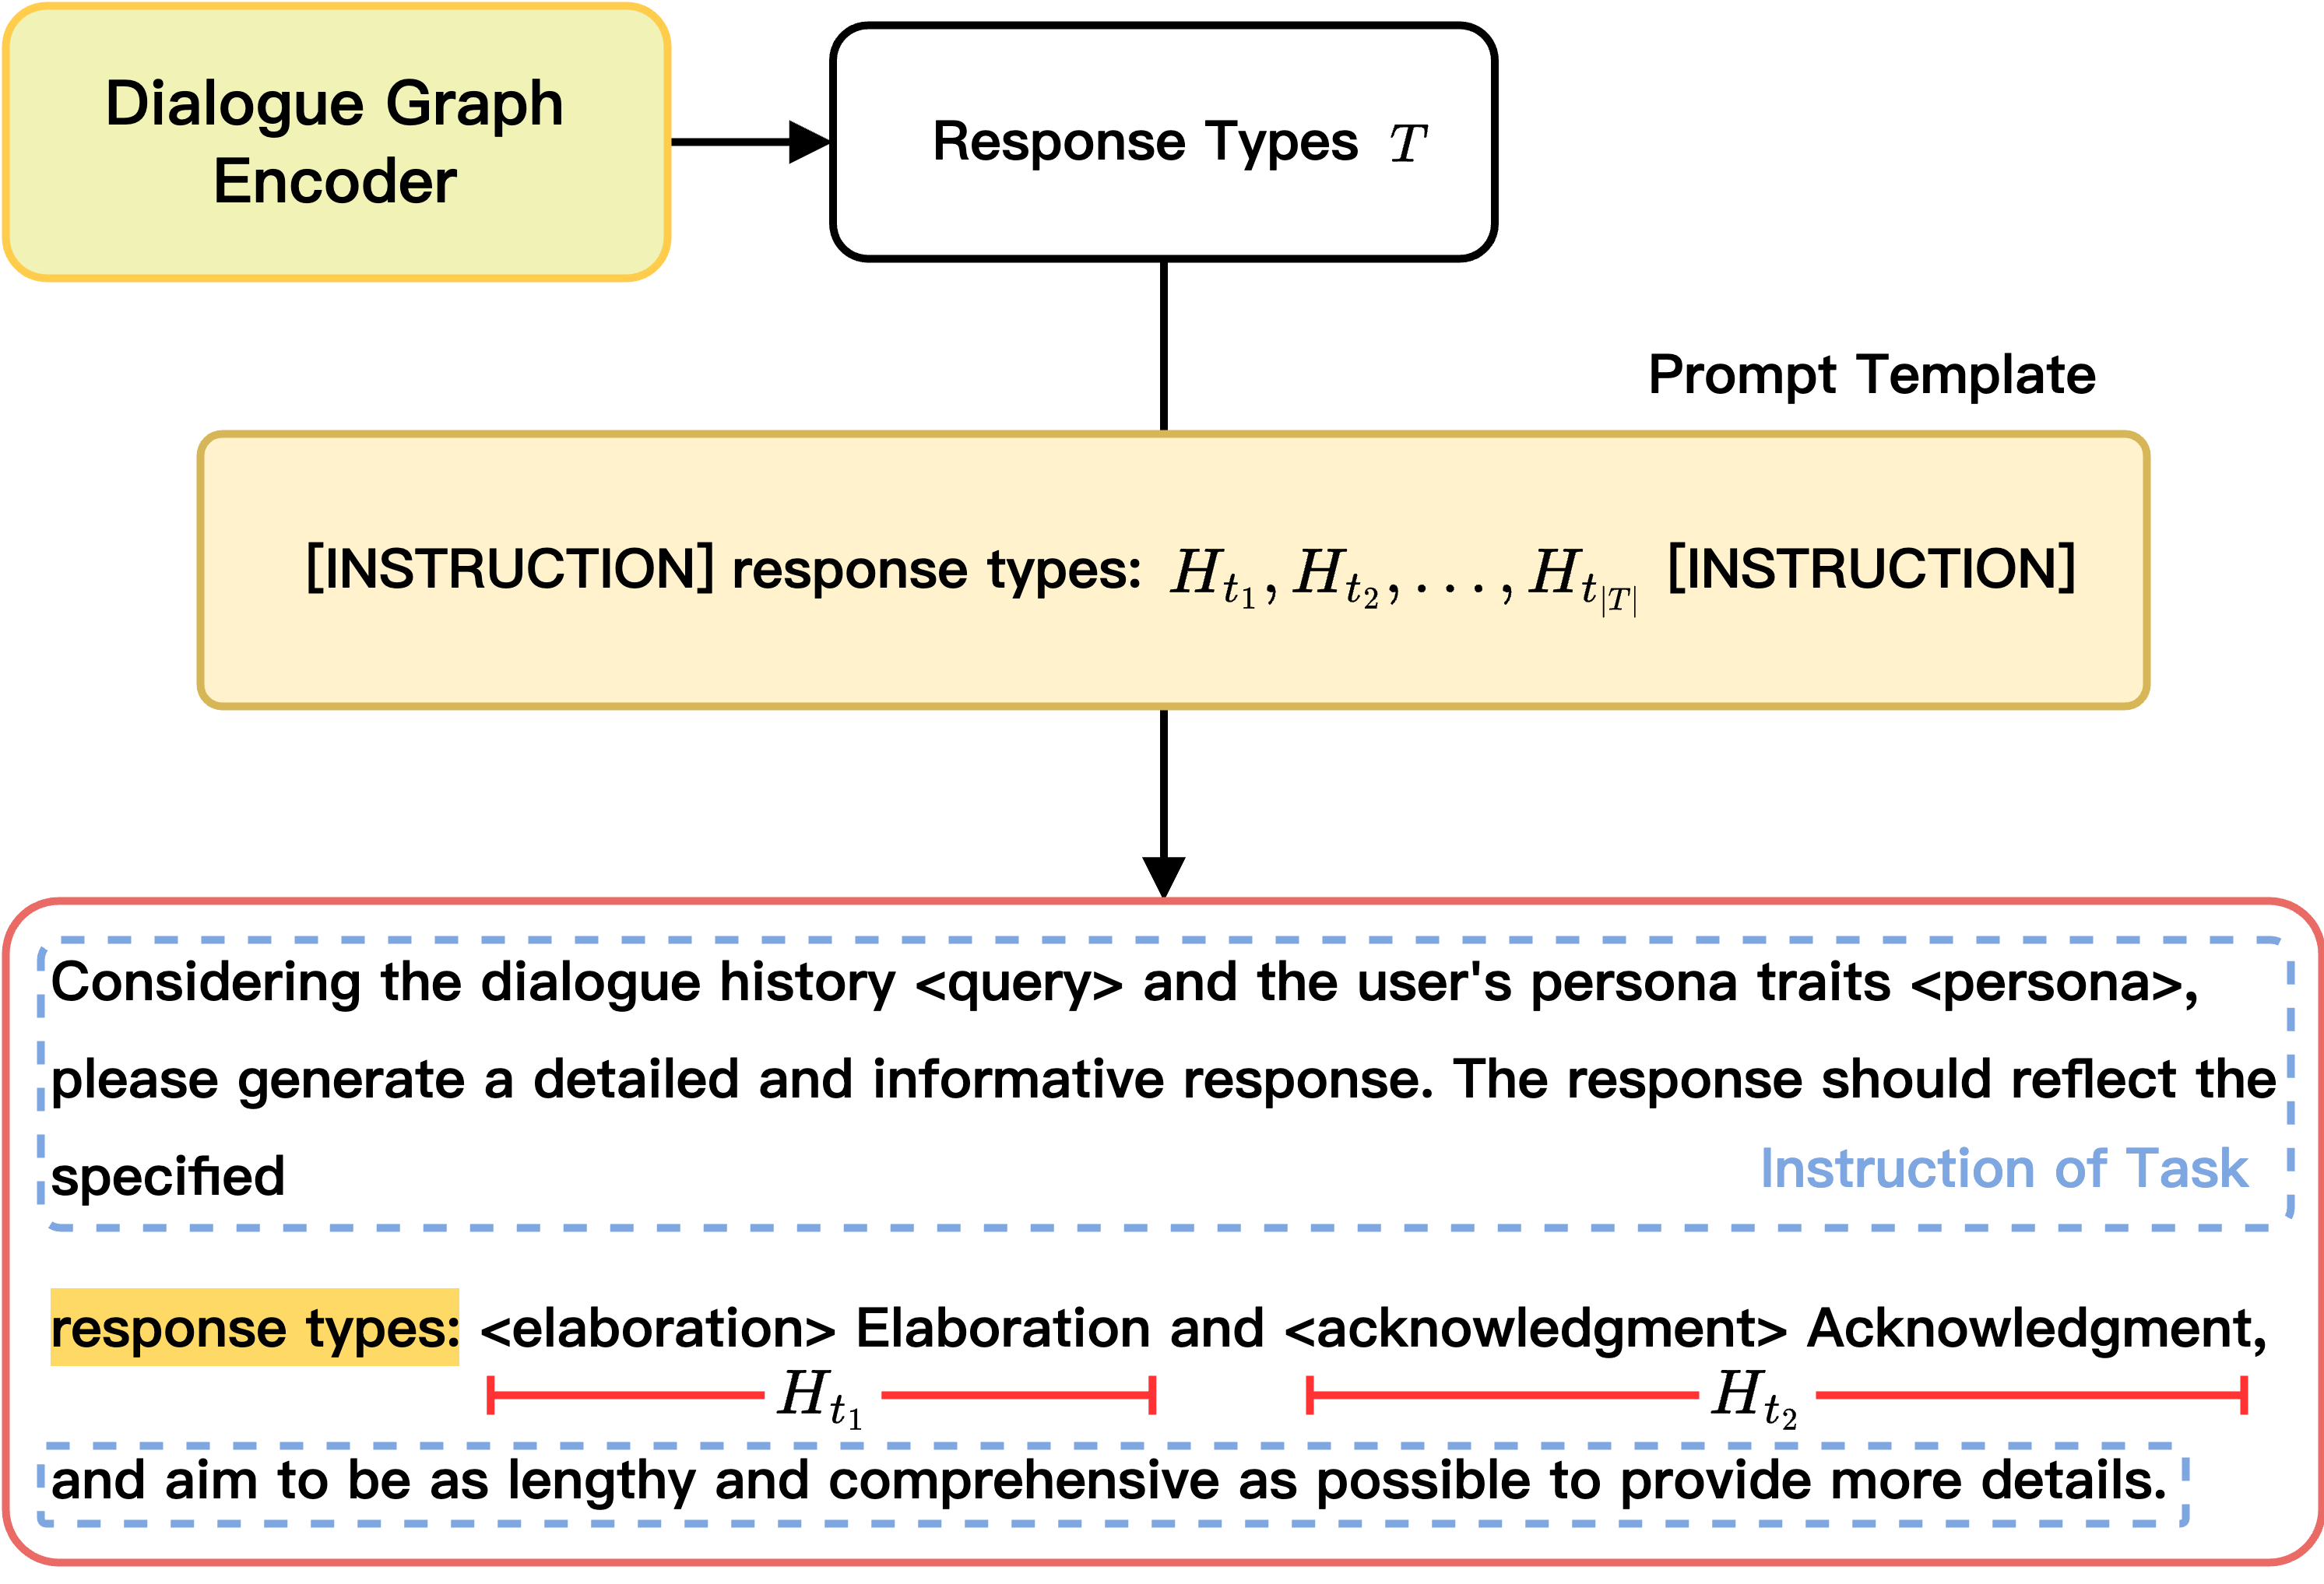
\includegraphics[width=1.00\textwidth]{./context/methodology/images/generator_prompt.png}
    \caption{The Prompt-Tuning pipeline. First, we utilize the dialogue graph encoder to process the context $C$ to predict the $top\text{-}k$ possible next response types $T$. Next, we integrate $T$ into the prompt template. The prompt not only mentions the desired response types but also includes instructions to generate responses, incorporating both persona and context information.}
    \label{fig:generator_prompt}
\end{figure}

Building on the next response type predictions of the Dialogue Graph Encoder, the Prompt Tuning module generates a comprehensive description. This description not only instructs the response generator on how to approach the given task but also guides its generation process by specifying the response types and leveraging both the dialogue context and the persona information.

Therefore, the input sequence for the personalized response generator (BART Decoder) is structured as follows:
\begin{align*}
    E_{\text{Generator}} = [e_{\text{[PROMPT]}}, e_{\text{[BOS]}}, e_{\text{[RSP]}}, e_{\text{1}}^{\text{k}}, e_{\text{2}}^{\text{k}}, ... , e_{\text{|K|-1}}^{\text{k}}, e_{\text{|K|}}^{\text{k}}, e_{\text{[EOS]}}]
\end{align*}

In an encoder-decoder transformer architecture like BART, the decoder references information from the encoder through cross-attention when predicting the next token. To ensure that the generator considers more coherence information while predicting the next token, we apply cross-attention to the dialogue representations generated by the previous two encoders at each transformer block. Thus, during the response generation process, each layer of the decoder performs cross-attention not only on the standard encoder outputs but also on the coherence-aware dialogue representation from the Dialogue Graph Encoder.

Additionally, we propose the Coherence-aware Attention mechanism. We first use learnable embeddings to capture the semantic information of coherence relations. Special tokens representing coherence relations are incorporated into the aforementioned prompt, combining the token embeddings of these special tokens with the coherence embeddings. This mechanism allows the generator to consider the type of response being predicted, such as selecting words that align with an Acknowledgment response type. The coherence-aware attention is visualized in Figure \ref{fig:coherence-aware_attention}. This dual cross-attention mechanism enables the decoder to leverage comprehensive context and persona information, thereby enhancing the coherence and personalization of the generated responses.

\begin{figure}[ht]
    \centering
    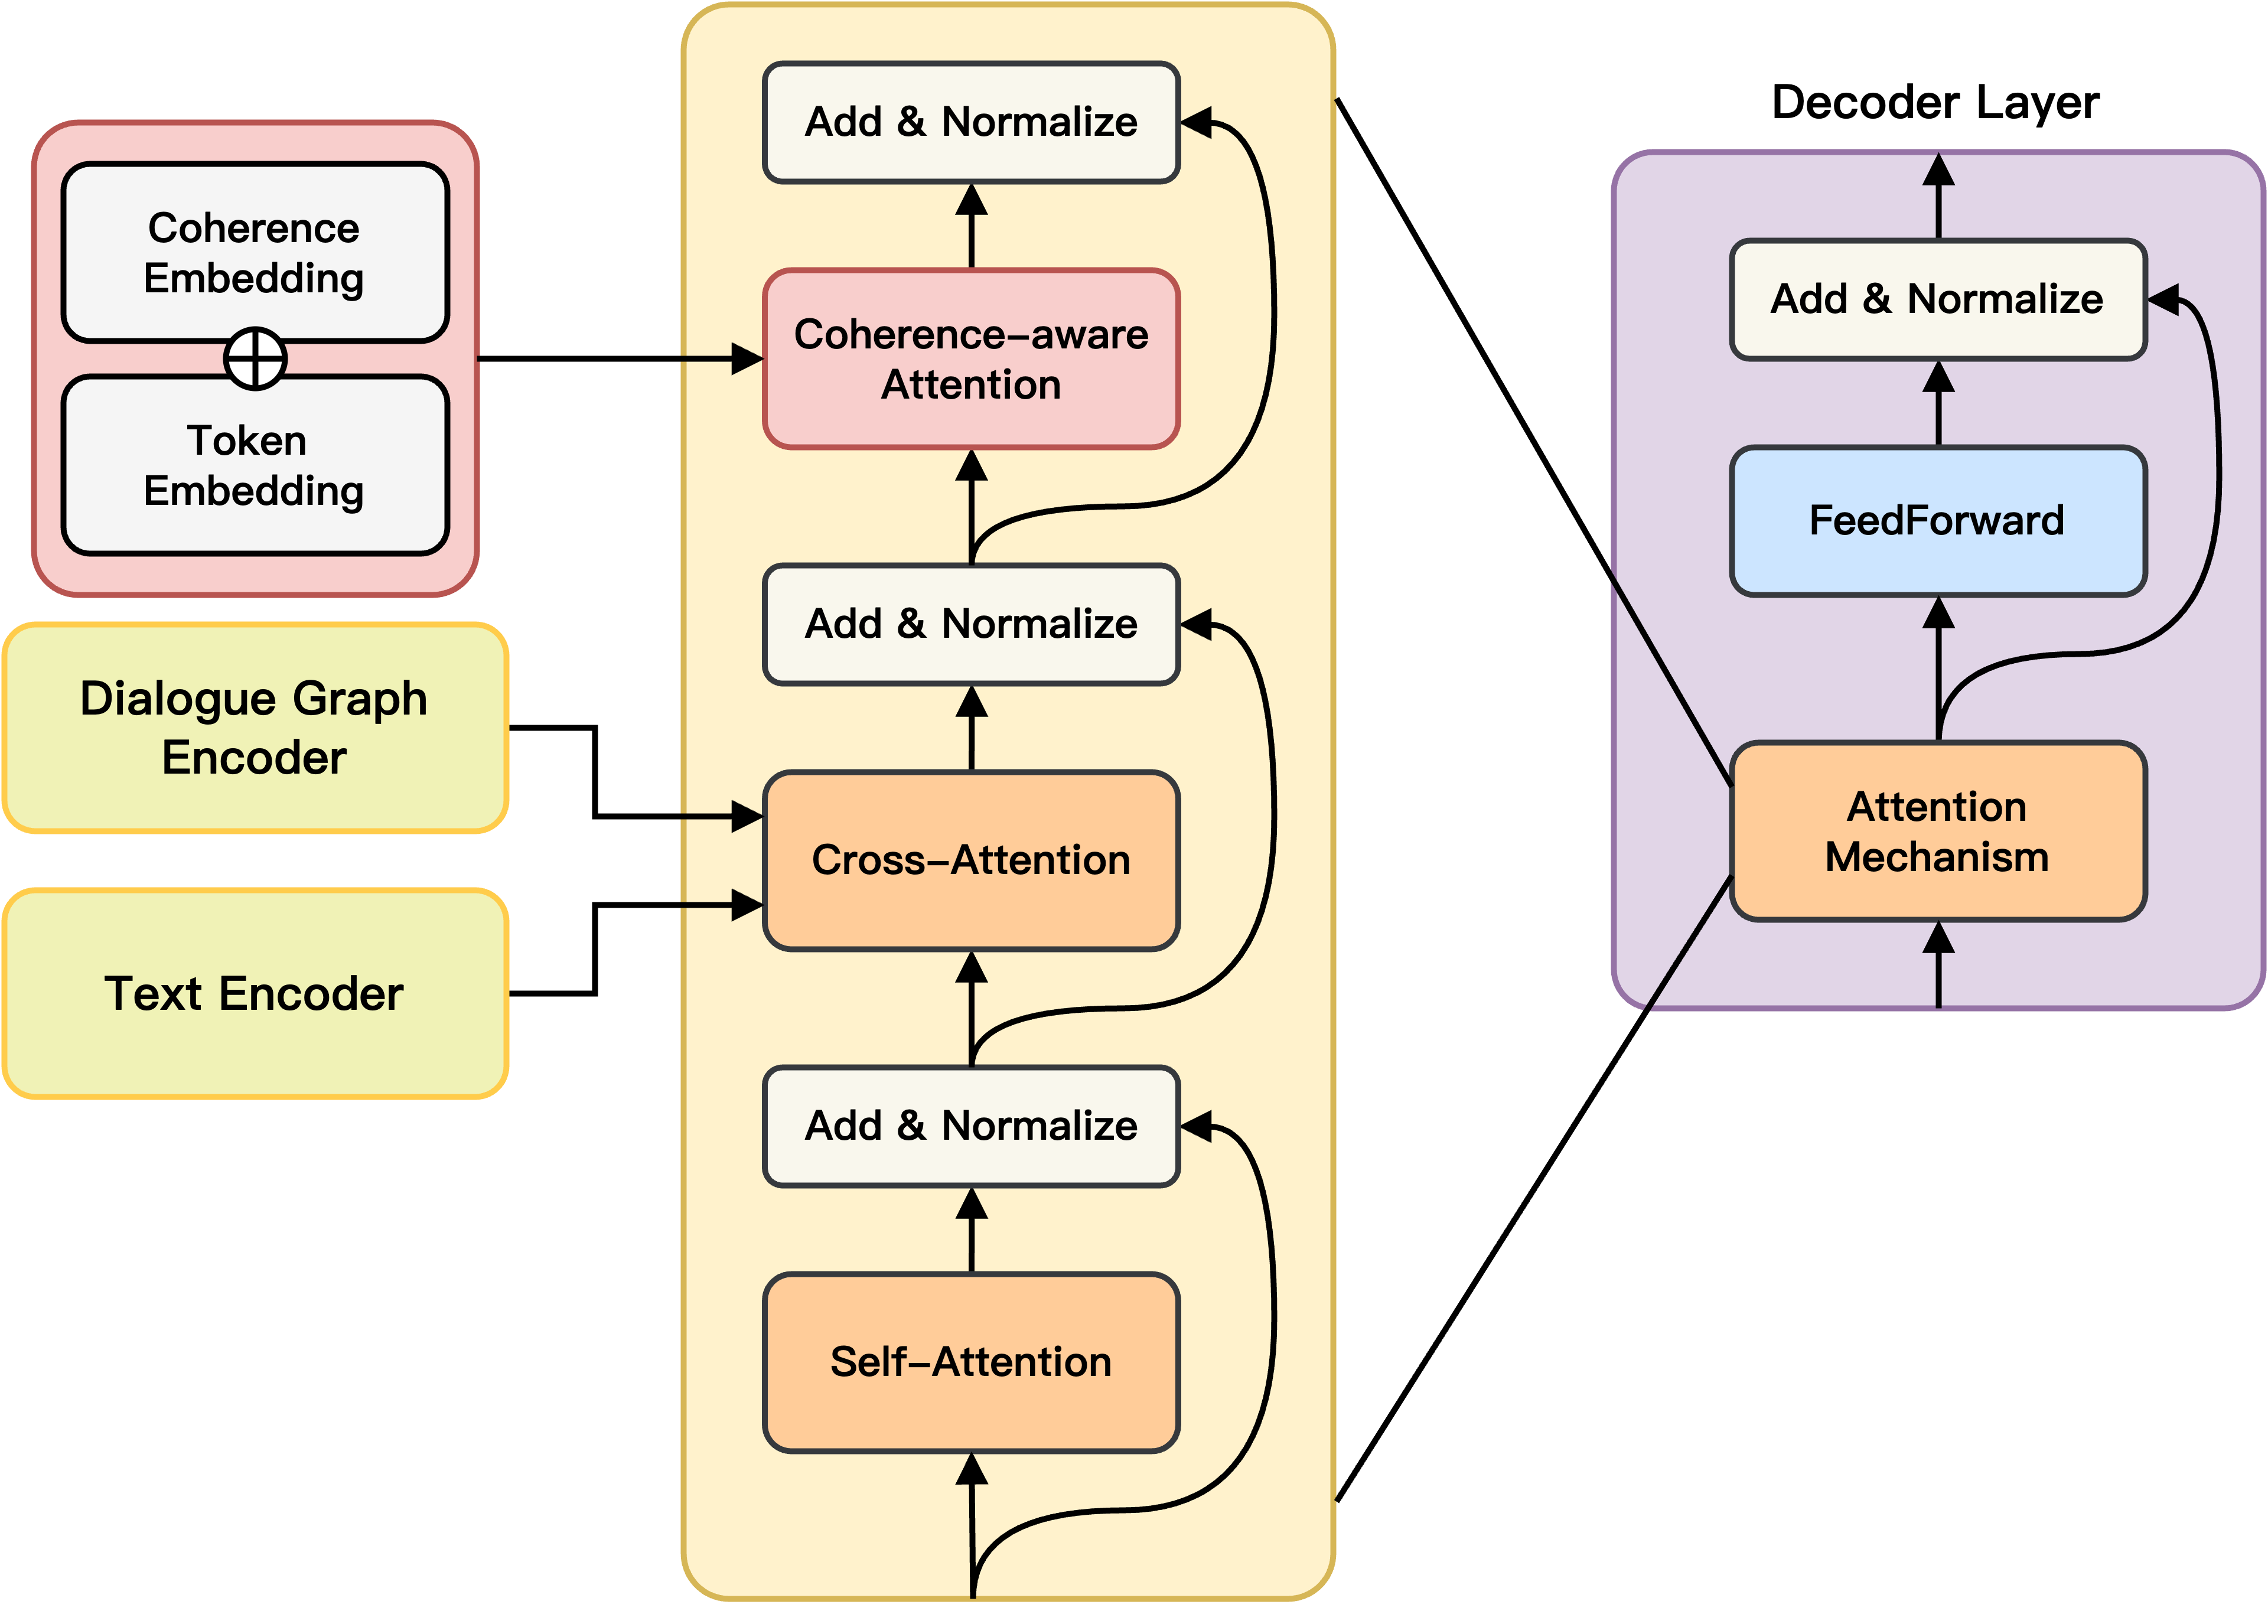
\includegraphics[width=1.00\textwidth]{./context/methodology/images/coherence-aware_attention.png}
    \caption{The visualizations of Coherence-aware Attention. We first compute the cross-attention between the encoder and decoder information. Then, we concatenate the coherence embedding and token embedding of the specified response type with this cross-attention result and perform coherence-aware attention to enrich the discourse information.}
    \label{fig:coherence-aware_attention}
\end{figure}

Finally, to enable the generator to better consider both persona-aware and coherence-aware context information during generation, we are inspired by \cite{huang-etal-2023-paa}. We fuse the decoder hidden states that consider the text encoder information with those that consider the dialogue graph encoder through a Dynamic Weighted Aggregation mechanism. Specifically, we compute a weight $w_{\text{TextEnc}}$ using a sigmoid function over the concatenated hidden states from both encoders (Eq. \ref{eq:dynamic_weighted_aggregation_weight}). Using this weight, we create masked versions of the encoder outputs based on a threshold hyperparameter $\tau$ to control the proportion of persona-aware and coherence-aware information to be considered (Eq. \ref{eq:dynamic_weighted_aggregation_weighting} and \ref{eq:dynamic_weighted_aggregation_mask}). The final output of the generator $O_{\text{Generator}}$ is obtained by adding a residual connection of the original encoder hidden states to the aggregated hidden states, enhancing the coherence and personalization of the generated responses. The detailed formulas are provided in the following equations:

\begin{equation} \label{eq:dynamic_weighted_aggregation_weight}
    w_{\text{TextEnc}} = \sigma(\text{MLP}([H_{\text{TextEnc}} \parallel H_{\text{GraphEnc}}]))
\end{equation}

\begin{equation} \label{eq:dynamic_weighted_aggregation_weighting}
    \begin{aligned}
        O_{\text{TextEnc}} &= w_{\text{TextEnc}} \cdot H_{\text{TextEnc}}, \\
        O_{\text{GraphEnc}} &= (1 - w_{\text{TextEnc}}) \cdot H_{\text{GraphEnc}}
    \end{aligned}
\end{equation}

\begin{equation} \label{eq:dynamic_weighted_aggregation_mask}
    \begin{aligned}
        m_{\text{TextEnc}} &= \mathbb{M}(w_{TextEnc} > \tau), \\
        m_{\text{GraphEnc}} &= \mathbb{M}(1 - w_{TextEnc} > \tau)
    \end{aligned}
\end{equation}

\begin{equation}
    \begin{aligned}
        \hat{O}_{\text{TextEnc}} &= m_{\text{TextEnc}} \odot O_{\text{TextEnc}}, \\
        \hat{O}_{\text{GraphEnc}} &= m_{\text{GraphEnc}} \odot O_{\text{GraphEnc}}, \\
        H_{\text{Enc}} &= \hat{O}_{\text{TextEnc}} + \hat{O}_{\text{GraphEnc}}
    \end{aligned}
\end{equation}

\begin{equation} \label{eq:dynamic_weighted_aggregation_output}
    \begin{aligned}
        H_{\text{residual}} &= H_{\text{TextEnc}} + H_{\text{GraphEnc}}, \\
        O_{\text{Generator}} &= H_{\text{Enc}} + H_{\text{residual}}
    \end{aligned}
\end{equation}

For personalized response generation, we use a language modeling task to compute the probability distribution over the vocabulary for generating the next word given the current context. The language modeling loss, typically implemented as the negative log-likelihood loss, is computed between the predicted probability distribution and the actual next word in the training data. This encourages the model to generate responses that are not only contextually appropriate but also aligned with the persona. The loss function can be formally defined as:

\begin{equation}
    \mathcal{L}_{\text{LM}} = - \sum_{t=1}^{T} \log P(y_t | y_{<t}, O_{\text{Generator}})
\end{equation}

By minimizing this loss function, the model learns to produce fluent and personalized responses that are coherent with the dialogue history and consistent with the persona.

% ------------------------------------------------
\EndChapter
% ------------------------------------------------


% Experiment chapter
% ------------------------------------------------
\StartChapter{Experiment}{chapter:experiment}
% ------------------------------------------------
This chapter presents an evaluation of our proposed methods for personalized dialogue generation. We conducted experiments on the ConvAI2 dataset. Our approach surpasses previous methods in multiple evaluative aspects of response generation, showcasing superior results in personalized dialogue generation.

\section{Datasets}
ConvAI2 \cite{dinan-etal-2019-convai2} is a chit-chat dataset based on PersonaChat \cite{zhang-etal-2018-personalizing}. The dataset comprises 17,878 and 1,000 multi-turn dialogues for the training and development sets, respectively, with a total of 131,438 and 7,801 utterances. It features 1,155 and 100 unique persona descriptions for the training and development sets, respectively. Each conversation participant who are assigned at least five persona descriptions, which are selected from these unique personas. Examples of the dialogue can be seen in Table \ref{table:convai2-example}.

\section{Baselines}
For comparison, we have selected the following baselines: (1) \textbf{Personalized Dialogue Generation methods}: We compare our approach with established text-description-based personalized models such as BOB \cite{song-etal-2021-bob}, LMEDR \cite{chen-etal-2023-memorize}, and PAA \cite{huang-etal-2023-paa}, which are recognized for their strong performance. (2) \textbf{General Dialogue Generation methods}: To ensure a fair evaluation, we include PLATO \cite{bao-etal-2020-plato} and DialoGPT \cite{zhang-etal-2019-dialogpt}. For PLATO, following the original publication's methodology, we prepend the persona descriptions as part of the knowledge to the entire context during inference. For DialoGPT, we adopt a post-processing approach as suggested by \cite{zhou-etal-2023-simoap}. We first generate multiple responses as candidates from DialoGPT for the same context and then select the response that is most consistent with the persona and most relevant to the context as the final output. (3) \textbf{Large Language Models (LLMs)}: We also test the ability of LLMs, specifically GPT-4, in personalized response generation, which utilizes prompting technologies. The prompt can be seen in Figure \ref{fig:llm_inference_prompt}.

% ----------------------------------------------
% Table: ConvAI2 Dataset Example
% ----------------------------------------------

\begin{table}[ht]
\centering
\def\arraystretch{1.4}%
\begin{tabular}{|p{7cm}|p{7cm}|}
\hline

\rowcolor[RGB]{204,217,245}
\multicolumn{1}{|c|}{\textbf{PERSON 1's Persona}} & \multicolumn{1}{|c|}{\textbf{PERSON 2's Persona}} \\
\hline
I like to ski. & I am an artist. \\
My wife does not like me anymore. & I have four children. \\
I have went to Mexico 4 times this year. & I recently got a cat. \\
I hate Mexican food. & I enjoy walking for exercise. \\
I like to eat cheetos. & I love watching Game of Thrones. \\
\hline

\rowcolor[RGB]{204,217,245}
\multicolumn{2}{|c|}{\textbf{Dialogue}} \\
\hline

\multicolumn{2}{|p{14cm}|}{[PERSON 1:] Hi} \\
\multicolumn{2}{|p{14cm}|}{[PERSON 2:] Hello ! How are you today?} \\
\multicolumn{2}{|p{14cm}|}{[PERSON 1:] I am good thank you , how are you.} \\
\multicolumn{2}{|p{14cm}|}{[PERSON 2:] Great, thanks ! My children and I were just about to watch Game of Thrones.} \\
\multicolumn{2}{|p{14cm}|}{[PERSON 1:] Nice! How old are your children?} \\
\multicolumn{2}{|p{14cm}|}{[PERSON 2:] I have four that range in age from 10 to 21. You?} \\
\multicolumn{2}{|p{14cm}|}{[PERSON 1:] I do not have children at the moment.} \\
\multicolumn{2}{|p{14cm}|}{[PERSON 2:] That just means you get to keep all the popcorn for yourself.} \\
\multicolumn{2}{|p{14cm}|}{[PERSON 1:] And Cheetos at the moment!} \\
\multicolumn{2}{|p{14cm}|}{[PERSON 2:] Good choice. Do you watch Game of Thrones?} \\
\multicolumn{2}{|p{14cm}|}{[PERSON 1:] No, I do not have much time for TV.} \\
\multicolumn{2}{|p{14cm}|}{[PERSON 2:] I usually spend my time painting. But, I love the show.} \\

\hline
\end{tabular}
\caption{Example dialogue from the ConvAI2 dataset. During training, the model acts as a conversational agent, playing the role of one of the participants to generate personalized responses.}
\label{table:convai2-example}
\end{table}

\section{Implementation Details}
The \textbf{MUDI} is mainly implemented in PyTorch. Our backbone Generator is BART-large\footnote[2]{https://huggingface.co/facebook/bart-large}. For Generator training, we train it using a batch size of 4 on 1 NVIDIA A100 80GB
GPU via the AdamW optimizer with a learning rate of \(5 \times 10^{-6}\) and a
weight decay of 0.01. For the Dialogue Graph Encoder training, it is conducted on a single NVIDIA RTX 4090 GPU using a batch size of 512. The training also employs the AdamW optimizer, but with a learning rate of \(2 \times 10^{-5}\) and the same weight decay of 0.01. In the Dialogue Graph Encoder, we initially employ the SBERT model "all-mpnet-base-v2"\footnote[3]{https://huggingface.co/sentence-transformers/all-mpnet-base-v2} to encode both the utterances and persona sentences, thereby initializing the node embeddings. We construct the Dialogue Graph by keeping the 3-hop neighbors. The model employs a 2-layer GNN with 4 multi-heads and a hidden dimension of 512. The weights for the different tasks are as follows: the weight of the Coherence Relation Classification task is 1.5, the weight of both types of Next Response Type Prediction tasks is 1.5, and the weight of the Link Prediction task is 1.2. For training the generator, we retain the most recent 5 turns of dialogue as historical context and choose the top-3 predicted response types for the prompt. We set \(\tau = 0.2\) for the Dynamic Weighted Aggregation.

\InsertFigure
[scale=0.46,
caption={The prompt of LLM inference on Personalized Dialogue Generation task.},
label={fig:llm_inference_prompt}
]
{./context/experiment/images/llm_inference_prompt.png}

\section{Evaluation Metrics}
\subsection{Automatic Metrics}
We assess the quality of dialogue responses from four perspectives: 

(1) \textbf{Text-similarity}: To evaluate the similarity between the generated responses and the ground-truth responses, we employ BLEU \cite{papineni-etal-2002-bleu} and ROUGE \cite{lin-2004-rouge} metrics, which focus on the word overlap level. Additionally, we utilize BERTScore \cite{zhang-etal-2020-bert-score}, which measures the semantic similarity between generated responses and ground-truth using contextual embeddings from BERT. This helps capture nuances that traditional overlap-based metrics might miss.

(2) \textbf{Diversity}: We assess the diversity and informativeness of the generated responses at token, sentence, and corpus levels. We utilize Distinct-n (Dist-$n$) metrics \cite{li-etal-2016-diversity} to measure the proportion of unique n-grams (n=1) relative to the total number of n-grams in the generated responses. Additionally, we employ Entropy-n (Ent-$n$) \cite{zhang-etal-2018-generating} to evaluate the uncertainty or randomness of the distribution of n-grams (n=1) in the generated text. We also calculate the Unique Sentence Ratio (USR) \cite{li-etal-2020-generate}, which quantifies text diversity by measuring the proportion of unique sentences among all predicted responses.

(3) \textbf{Coherence}: Previous studies often omit explicit evaluations of Coherence, assuming that Fluency can also measure the coherence of dialogues. However, this approach does not directly account for the coherence of generated responses with the context and query, an aspect often presumed to be covered by fluency. To measure this unexplored dimension, our research incorporates specific coherence metrics to provide a more accurate and holistic assessment of response quality. Specifically, we employ several metrics. Firstly, we use QuantiDCE \cite{ye-etal-2021-towards-quantifiable} and DEAM \cite{ghazarian-etal-2022-deam}, which are state-of-the-art metrics in dialogue coherence evaluation. These metrics assess both how logically the responses align with the preceding query or the entire context within the dialogue, and how well the utterances in a conversation are unified, leading to a consistent and coherent interaction. Additionally, we utilize BARTScore \cite{yuan-etal-2021-bartscore} to measure coherence under the faithfulness setting discussed in the paper.

(4) \textbf{Personalization}: To assess the personalization of the generated responses, we first measure the alignment between the persona and responses. First, we apply Consistency Score (C.Score) \cite{madotto-etal-2019-personalizing}, which leverages a NLI model to predict consistency between response and persona. Additionally, we utilize the BARTScore \cite{yuan-etal-2021-bartscore}, which provides a method to calculate the semantic overlaps between texts. Specifically, we compute: (a) Precision (persona → response): This measures how closely the generated responses adhere to the input persona, reflecting the degree to which the model captures persona-specific attributes in the response. (b) Recall (response → persona): This assesses whether all aspects of the persona are sufficiently covered by the responses, indicating the comprehensiveness of the persona information in the generated text. we report the F1 Score is then calculated from these Precision and Recall scores to provide a balanced measure of personalization, capturing both the accuracy and completeness of the generated responses in reflecting the specified persona.

Moreover, to better assess whether the generated responses accurately incorporate important features from the persona or the query, we utilize Large Language Models (LLMs)\footnote[4]{https://huggingface.co/meta-llama/Meta-Llama-3-70B-Instruct} to identify key terms (features) from these persona descriptions or dialogue utterances. We then employ a NLI model to calculate the Feature Coverage Ratio (FCR), ensuring that critical features are effectively represented in the responses. The example of the feature-annotated table mentioned earlier is shown in Table \ref{table:fcr-feature-annotated-example}.

\begin{table}[H]
\centering
\def\arraystretch{1.2}%
\begin{tabular}{|l|c|}
\hline

\rowcolor[RGB]{204,217,245}
\multicolumn{1}{|c|}{\textbf{Persona description}} & \textbf{Features} \\
\hline

I read twenty books a year. & read books, twenty books a year   \\
\hline

I'm a stunt double as my second job. & stunt double, second job \\
\hline

I only eat kosher. & only eat kosher \\
\hline

I was raised in a single parent household. & single parent household \\
\hline

\rowcolor[RGB]{204,217,245}
\multicolumn{1}{|c|}{\textbf{Utterance}} & \textbf{Features} \\
\hline

Oh wow. All i've is a dog. That's enough for me. & having a dog  \\
\hline

I am good, I just got off work and tired, I have two jobs. & got off work, two jobs, tired \\
\hline

But a good movie is always good. & good movie \\
\hline

\end{tabular}
\caption{Examples of feature annotations used for calculating the Feature Coverage Ratio (FCR). All personas and queries in the dialogue have been annotated.}
\label{table:fcr-feature-annotated-example}
\end{table}

\section{Main Results}
Apart from DialoGPT, we use the context of the most recent 5 turns as dialogue history. After testing, we found that DialoGPT starts to talk nonsense when given more than 2 turns of context. Therefore, for DialoGPT, we only use the most recent 2 turns.

In Table \ref{table:text-similarity}, we report experimental results on Text Similarity evaluation. Our method offers better BLEU, ROUGE, and BERTScore compared with baseline methods. Specifically, MUDI's BLEU-1, ROUGE-1, and ROUGE-L scores reach 18.19, 17.10, and 16.13, respectively, outperforming existing methods by 1.64, 3.57, and 3.45. As shown in Table \ref{table:text-diversity}, we report the Diversity evaluation. MUDI's USR is 1.0, indicating that it can generate completely unique responses under different queries and personas. Additionally, we achieved the second-highest scores in Ent-1 and Dist-1. Upon examining the outputs from PLATO, we found that they often generate shorter sentences, such as 'me to!!'. Shorter sentences tend to inflate certain metrics, like Dist-1, because they typically involve less repetition of words within a single response, leading to high distinct scores. This suggests that while our method ranks second, it could provide more substantial and contextually rich responses compared to PLATO. Furthermore, our approach achieves the highest scores among all Persona-based dialogue generation methods and significantly surpasses other baselines in Dist-1, outperforming them by 7.95. This performance establishes our method could generate varied and engaging responses.

In addition, Table \ref{table:coherence} presents the results of the Coherence evaluation. Compared to other persona-based methods, MUDI has made significant progress in QuantiDCE, DEAM, and BARTScore, particularly in assessing the coherence between the query and response (left-side scores). This indicates that our approach indeed enables the model to generate responses with enhanced local coherence. Furthermore, MUDI also achieves excellent results in global coherence, which evaluates the coherence between the entire dialogue context and the response (right-side scores).

Finally, Table \ref{table:personalization} presents the results of evaluating Personalization and Feature Coverage. PAA significantly outperforms other methods in scores for Personalization and FCR$_p$. Upon further examination, we discovered that this is because PAA frequently generates sentences that are exact restatements of the persona description, often ignoring the relevance to the query. As a result, its high scores in Personalization can be attributed to this tendency. Excluding the special case of PAA, MUDI achieves excellent results in Personalization compared to other methods. Combined with the previously discussed results from the Coherence evaluation (Table \ref{table:personalization}), this demonstrates that our approach successfully balances discourse relations and persona. It generates responses that effectively consider both aspects simultaneously. Furthermore, our model achieves comparable scores in the Coherence evaluation compared to DialoGPT, which focuses on general dialogue generation.

In evaluating powerful LLMs like GPT-4, we find that they excel at generating lengthy responses and maintaining coherence between questions and dialogue context. Consequently, GPT-4 stands out in Coherence evaluation, scores highly in Ent-1, and performs well in FCR$_q$. However, this also results in a lower overlap with the ground-truth responses, leading to lower Text Similarity scores. Moreover, the longer sentences generated lead to a lower Dist-1 score. Another observation is that GPT-4 performs well in tasks related to Personalization, which confirms the robust capabilities of large-parameter LLMs. Additionally, when we provide LLMs with information on coherence relations, there is an observed improvement in FCR evaluations. This suggests that appropriate response type guidance can focus the LLM more on the important aspects of the questions, thus making it easier for the model to generate sentences that are relevant to the persona. However, previous research \cite{deshpande-etal-2023-toxicity} suggests that using LLMs for personalized dialogue generation can encounter biases in the generated content, which still requires careful consideration.

In summary, compared to existing methods, our approach MUDI not only significantly improves performance in Text Similarity scores but also excels at integrating discourse relations and persona information. This enables us to generate personalized responses that are not only rich in content and diverse but also encompass these aspects. Moreover, in Coherence evaluations, our method achieves scores comparable to those of state-of-the-art models specialized in open-domain dialogue generation.

% ----------------------------------------------
% Table 1: Text Similarity
% ----------------------------------------------

\begin{table}[H]
\centering
\def\arraystretch{1.3}%
\begin{tabular}{|c|c|c|c|c|c|c|}
\hline
\multicolumn{2}{|c|}{\multirow{2}{*}{\textbf{Model}}}  & \multicolumn{5}{c|}{\textbf{Text Similarity}} \\
\cline{3-7}

\multicolumn{2}{|c|}{} & BLEU-1 $\uparrow$ & BLEU-2 $\uparrow$ & ROUGE-1 $\uparrow$ & ROUGE-L $\uparrow$ & BERTScore $\uparrow$ \\
\hhline{|=======|}

\rowcolor[RGB]{242,164,100}
\multicolumn{7}{|c|}{\textbf{Large Language Model (Prompting)}} \\
\hhline{|=======|}

\multicolumn{2}{|c|}{\textbf{GPT-4}} &7.47 &2.40 &13.52 &11.06 &84.05 \\ 
\hhline{|=======|}

\rowcolor{yellow}
\multicolumn{7}{|c|}{\textbf{General Dialogue Generation}} \\
\hhline{|=======|}

\multicolumn{2}{|c|}{\textbf{DialoGPT}} &7.34	&1.54 &9.46 &8.41 &83.31 \\ 
\hline

\multirow{2}{*}{\textbf{PLATO}} & w/ persona &4.35	&1.01 &4.88 &4.80 &82.77 \\ 
\cline{2-7}

\multirow{2}{*}{\textbf{}} & w/o persona  &6.82 &1.86 &4.99 &4.77 &81.44 \\ 
\hhline{|=======|}

\rowcolor[RGB]{204,217,245}
\multicolumn{7}{|c|}{\textbf{Persona-based Dialogue Generation}} \\
\hhline{|=======|}

\multicolumn{2}{|c|}{\textbf{BoB}} &15.30 &5.39 &13.21 &12.48 &83.77 \\ 
\hline

% \multicolumn{2}{|c|}{\textbf{P$^{2}$BOT}} &- &- &- &- &- \\ 
% \hline

\multicolumn{2}{|c|}{\textbf{LMEDR}}		&15.47	&5.83	&13.28	&12.26	&85.00 \\ 
\hline

\multicolumn{2}{|c|}{\textbf{PAA}}          &\underline{16.55}    &6.28    &13.53 
&12.68    &84.42   \\
\hline

\multirow{3}{*}{\textbf{\begin{tabular}{@{}c@{}}MUDI \\ (ours)\end{tabular}}} &SP\textsubscript{$\tau=0.2$}	&15.14	&6.43	&14.87	&13.87	&85.07	\\
\cline{2-7}

\multirow{3}{*}{} &Emb\textsubscript{$\tau=0.2$}   &\underline{16.55}    &\underline{7.34}	&\textbf{\textcolor{red}{17.10}}	&\textbf{\textcolor{red}{16.13}}	&\underline{85.42}	\\
\cline{2-7}

\multirow{3}{*}{} &SP+Emb\textsubscript{$\tau=0.2$}   &\textbf{\textcolor{red}{18.19}} &\textbf{\textcolor{red}{7.77}}	&\underline{16.59}	&\underline{15.46}	&\textbf{\textcolor{red}{85.53}} \\
\hline
\end{tabular}
\caption{Automatic evaluation results on ConvAI2 dataset over our implemented approach. The best results in each column are in bold, while the second is underlined.}
\label{table:text-similarity}
\end{table}

% ----------------------------------------------
% Table 2: Diversity
% ----------------------------------------------

\begin{table}[H]
\centering
\def\arraystretch{1.3}%
\begin{tabular}{|c|c|c|c|c|}
\hline
\multicolumn{2}{|c|}{\multirow{2}{*}{\textbf{Model}}}  &\multicolumn{3}{c|}{\textbf{Diversity}}\\
\cline{3-5}

\multicolumn{2}{|c|}{} &Ent-1 $\uparrow$ &Dist-1 $\uparrow$ &USR $\uparrow$ \\
\hhline{|=====|}

\rowcolor[RGB]{242,164,100}
\multicolumn{5}{|c|}{\textbf{Large Language Model (Prompting)}} \\
\hhline{|=====|}

\multicolumn{2}{|c|}{\textbf{GPT-4}} &9.40 &16.09 &1.00 \\ 
\hhline{|=====|}

\rowcolor{yellow}
\multicolumn{5}{|c|}{\textbf{General Dialogue Generation}} \\
\hhline{|=====|}

\multicolumn{2}{|c|}{\textbf{DialoGPT}} &\textbf{\textcolor{red}{9.05}} &36.84 &\underline{0.99} \\ 
\hline

\multirow{2}{*}{\textbf{PLATO}} & w/ persona &4.67 &\textbf{\textcolor{red}{58.18}} &0.61 \\ 
\cline{2-5}

\multirow{2}{*}{\textbf{}} & w/o persona &6.73 &43.34 &0.85 \\ 
\hhline{|=====|}

\rowcolor[RGB]{204,217,245}
\multicolumn{5}{|c|}{\textbf{Persona-based Dialogue Generation}} \\
\hhline{|=====|}


\multicolumn{2}{|c|}{\textbf{BoB}} &7.89 &41.75 &\underline{0.99} \\ 
\hline

% \multicolumn{2}{|c|}{\textbf{P$^{2}$BOT}} &- &- &- \\ 
% \hline

\multicolumn{2}{|c|}{\textbf{LMEDR}}  &7.14	&43.08	&0.94\\ 
\hline

\multicolumn{2}{|c|}{\textbf{PAA}}    &6.66	&40.27  &0.87 \\
\hline

\multirow{3}{*}{\textbf{\begin{tabular}{@{}c@{}}MUDI \\ (ours)\end{tabular}}} &SP\textsubscript{$\tau=0.2$}	&\underline{8.13}		&46.76	&\textbf{\textcolor{red}{1.00}}\\
\cline{2-5}

\multirow{3}{*}{} &Emb\textsubscript{$\tau=0.2$}   &7.65	&\underline{51.03}	&\textbf{\textcolor{red}{1.00}}\\
\cline{2-5}

\multirow{3}{*}{} &SP+Emb\textsubscript{$\tau=0.2$} 	&7.66	&47.68  &\textbf{\textcolor{red}{1.00}}\\
\hline
\end{tabular}
\caption{Automatic evaluation results for diversity tested on ConvAI2 dataset over our implemented approach. The best results in each column are in bold, while the second is underlined.}
\label{table:text-diversity}
\end{table}

% ----------------------------------------------
% Table 3: Coherence 
% ----------------------------------------------

\begin{table}[H]
\centering
\def\arraystretch{1.3}%
\begin{tabular}{|c|c|c|c|c|}
\hline
\multicolumn{2}{|c|}{\multirow{2}{*}{\textbf{Model}}}  & \multicolumn{3}{c|}{\textbf{Coherence}} \\
\cline{3-5}

\multicolumn{2}{|c|}{} & QuantiDCE $\uparrow$ & DEAM $\uparrow$ & BARTScore$_{q \rightarrow r, c \rightarrow r}$ $\downarrow$ \\
\hline

\multicolumn{2}{|c|}{\textbf{GOLD}}          &3.19 / 2.83    &0.64 / 0.85    &5.74 / 5.70   \\
\hhline{|=====|}

\rowcolor[RGB]{242,164,100}
\multicolumn{5}{|c|}{\textbf{Large Language Model (Prompting)}} \\
\hhline{|=====|}

\multirow{2}{*}{\textbf{GPT-4}} & w/ coherence relations  &3.40 / 2.91 &0.77 / 0.95 &4.27 / 3.74 \\ 
\cline{2-5}
\multirow{2}{*}{\textbf{}} & w/o coherence relations  &3.41 / 2.92 &0.87 / 0.96 &4.24 / 3.73 \\ 

\hhline{|=====|}

\rowcolor{yellow}
\multicolumn{5}{|c|}{\textbf{General Dialogue Generation}} \\
\hhline{|=====|}

\multicolumn{2}{|c|}{\textbf{DialoGPT}} &\textbf{\textcolor{red}{3.23}} / 2.79 &\textbf{\textcolor{red}{0.70}} / \textbf{\textcolor{red}{0.88}} &5.12 / 5.19 \\ 
\hline

% \multirow{2}{*}{\textbf{PLATO}} & w/ persona &3.32 / 3.43	&0.22 / 0.75 &6.42 / 6.63 \\ 
\multirow{2}{*}{\textbf{PLATO}} & w/ persona &1.68 / 1.57	&0.22 / 0.75 &6.42 / 6.63 \\ 
\cline{2-5}

\multirow{2}{*}{\textbf{}} & w/o persona  &1.87 / 1.77 &0.25 / 0.74 &5.83 / 5.80 \\ 
\hhline{|=====|}

\rowcolor[RGB]{204,217,245}
\multicolumn{5}{|c|}{\textbf{Persona-based Dialogue Generation}} \\
\hhline{|=====|}

\multicolumn{2}{|c|}{\textbf{BoB}} &2.99 / 2.76 &0.39 / 0.86 &5.82 / 5.92 \\ 
\hline

% \multicolumn{2}{|c|}{\textbf{P$^{2}$BOT}} &- &- &- \\ 
% \hline

\multicolumn{2}{|c|}{\textbf{LMEDR}}		&2.89 / 2.90	&0.43 / 0.78	&5.32 / 4.99  \\ 
\hline

\multicolumn{2}{|c|}{\textbf{PAA}}           &2.70 / \underline{2.93}    &0.56 / 0.83    &5.17 / \underline{4.62}   \\
\hline

\multirow{3}{*}{\textbf{\begin{tabular}{@{}c@{}}MUDI \\ (ours)\end{tabular}}} &SP\textsubscript{$\tau=0.2$}	&3.05 / 2.84	&0.63 / 0.85	&\underline{4.67} / \textbf{\textcolor{red}{4.61}}	\\
\cline{2-5}

\multirow{3}{*}{} &Emb\textsubscript{$\tau=0.2$}   &\textbf{\textcolor{red}{3.23}} / \textbf{\textcolor{red}{2.94}}    &0.56 / 0.82	&4.80 / 4.83 \\
\cline{2-5}

\multirow{3}{*}{} &SP+Emb\textsubscript{$\tau=0.2$}   &\underline{3.21} / 2.92	&\underline{0.64} / \underline{0.86}	&\textbf{\textcolor{red}{4.66}} / 4.66	\\
\hline
\end{tabular}
\caption{Automatic evaluation results for coherence tested on the ConvAI2 dataset. The best results in each column are in bold, while the second-best results are underlined. The score on the left considers only the local coherence between the query and the response, while the score on the right takes into account the global coherence between the entire dialogue and the response.}
\label{table:coherence}
\end{table}

% ----------------------------------------------
% Table 4: Personalization & Feature Coverage
% ----------------------------------------------

\begin{table}[H]
\centering
\def\arraystretch{1.3}%
\begin{tabular}{|c|c|c|c|c|c|}
\hline
\multicolumn{2}{|c|}{\multirow{2}{*}{\textbf{Model}}}  &\multicolumn{2}{c|}{\textbf{Personalization}} &\multicolumn{2}{c|}{\textbf{Feature Coverage}}\\
\cline{3-6}

\multicolumn{2}{|c|}{} &C.Score $\uparrow$ &BARTScore$_{p \leftrightarrow r}$ $\downarrow$ &FCR$_{q}$ $\uparrow$ &FCR$_{p}$ $\uparrow$ \\
\hline

\multicolumn{2}{|c|}{\textbf{GOLD}}      &4.10   &5.68 &7.69 &4.52 \\
\hhline{|======|}

\rowcolor[RGB]{242,164,100}
\multicolumn{6}{|c|}{\textbf{Large Language Model (Prompting)}} \\
\hhline{|======|}

\multirow{2}{*}{\textbf{GPT-4}} & w/ coherence relations  &29.47 &4.33 &21.62 &27.12 \\ 
\cline{2-6}
\multirow{2}{*}{\textbf{}} & w/o coherence relations  &28.90 &4.07 &9.77 &5.72 \\ 
\hhline{|======|}

\rowcolor{yellow}
\multicolumn{6}{|c|}{\textbf{General Dialogue Generation}} \\
\hhline{|======|}

\multicolumn{2}{|c|}{\textbf{DialoGPT}} &4.53 &5.39 &\textbf{\textcolor{red}{6.78}} &4.45  \\ 
\hline

\multirow{2}{*}{\textbf{PLATO}} & w/ persona &0.56 &6.06 &1.20 &0.92 \\ 
\cline{2-6}

\multirow{2}{*}{\textbf{}} & w/o persona  &0.18 &5.83 &3.23 &0.28 \\ 
\hhline{|======|}

\rowcolor[RGB]{204,217,245}
\multicolumn{6}{|c|}{\textbf{Persona-based Dialogue Generation}} \\
\hhline{|======|}

\multicolumn{2}{|c|}{\textbf{BoB}} &0.51 &5.52 &3.68 &0.42  \\ 
\hline

% \multicolumn{2}{|c|}{\textbf{P$^{2}$BOT}} &- &- &- &-  \\ 
% \hline

\multicolumn{2}{|c|}{\textbf{LMEDR}}		&7.38	&5.27 &4.63	 &6.99 \\ 
\hline


\multicolumn{2}{|c|}{\textbf{PAA}}       &\textbf{\textcolor{red}{15.19}}   &\textbf{\textcolor{red}{4.26}} &\underline{4.66}    &\textbf{\textcolor{red}{13.84}} \\
\hline

\multirow{3}{*}{\textbf{\begin{tabular}{@{}c@{}}MUDI \\ (ours)\end{tabular}}} &SP\textsubscript{$\tau=0.2$}	&\underline{11.87} &\underline{4.53} &\underline{4.66} &6.50	\\
\cline{2-6}

\multirow{3}{*}{} &Emb\textsubscript{$\tau=0.2$}   &9.70	&4.75 &4.36 &\underline{7.77} \\
\cline{2-6}

\multirow{3}{*}{} &SP+Emb\textsubscript{$\tau=0.2$}  &9.75	&4.76 &4.05 &5.01 \\
\hline
\end{tabular}
\caption{Automatic evaluation results for personalization and feature coverage tested on the  ConvAI2 dataset. The best results in each column are in bold, while the second-best results are underlined.}
\label{table:personalization}
\end{table}

% ----------------------------------------------
% Section: Analysis
% ----------------------------------------------

\section{Analysis}

\subsection{The Effect of Proposed DialogueGAT}
To validate the performance of the proposed DialogueGAT compared with existing GNN methods in Dialogue Graph modeling, we analyze results in the Next Response Type Prediction (NRTP) and Coherence Relations Classification tasks on the validation set. We compare DialogueGAT with GATv2. This comparison is illustrated in Figure \ref{fig:compare_gatv2_dialoguegat}. The experimental results demonstrate that DialogueGAT consistently outperforms GATv2 across all tasks in terms of Hits@5 scores, highlighting its enhanced capability to predict discourse relations (response types) from dialogue context information. Notably, in the Coherence Relations Classification (RC) task, DialogueGAT achieves significant improvements, showcasing its robustness in understanding context relationships. Additionally, the loss metrics further validate the efficiency of DialogueGAT; it registers lower loss values than GATv2 in both NRTP tasks, indicating superior model optimization and better fitting. The most pronounced difference is observed in the RC task, where the loss for DialogueGAT is markedly lower, emphasizing its exceptional performance in accurately classifying coherence relations. These findings suggest that DialogueGAT enhances prediction accuracy and effectively reduces error rates in discourse understanding.

\begin{figure}[H]
    \centering
    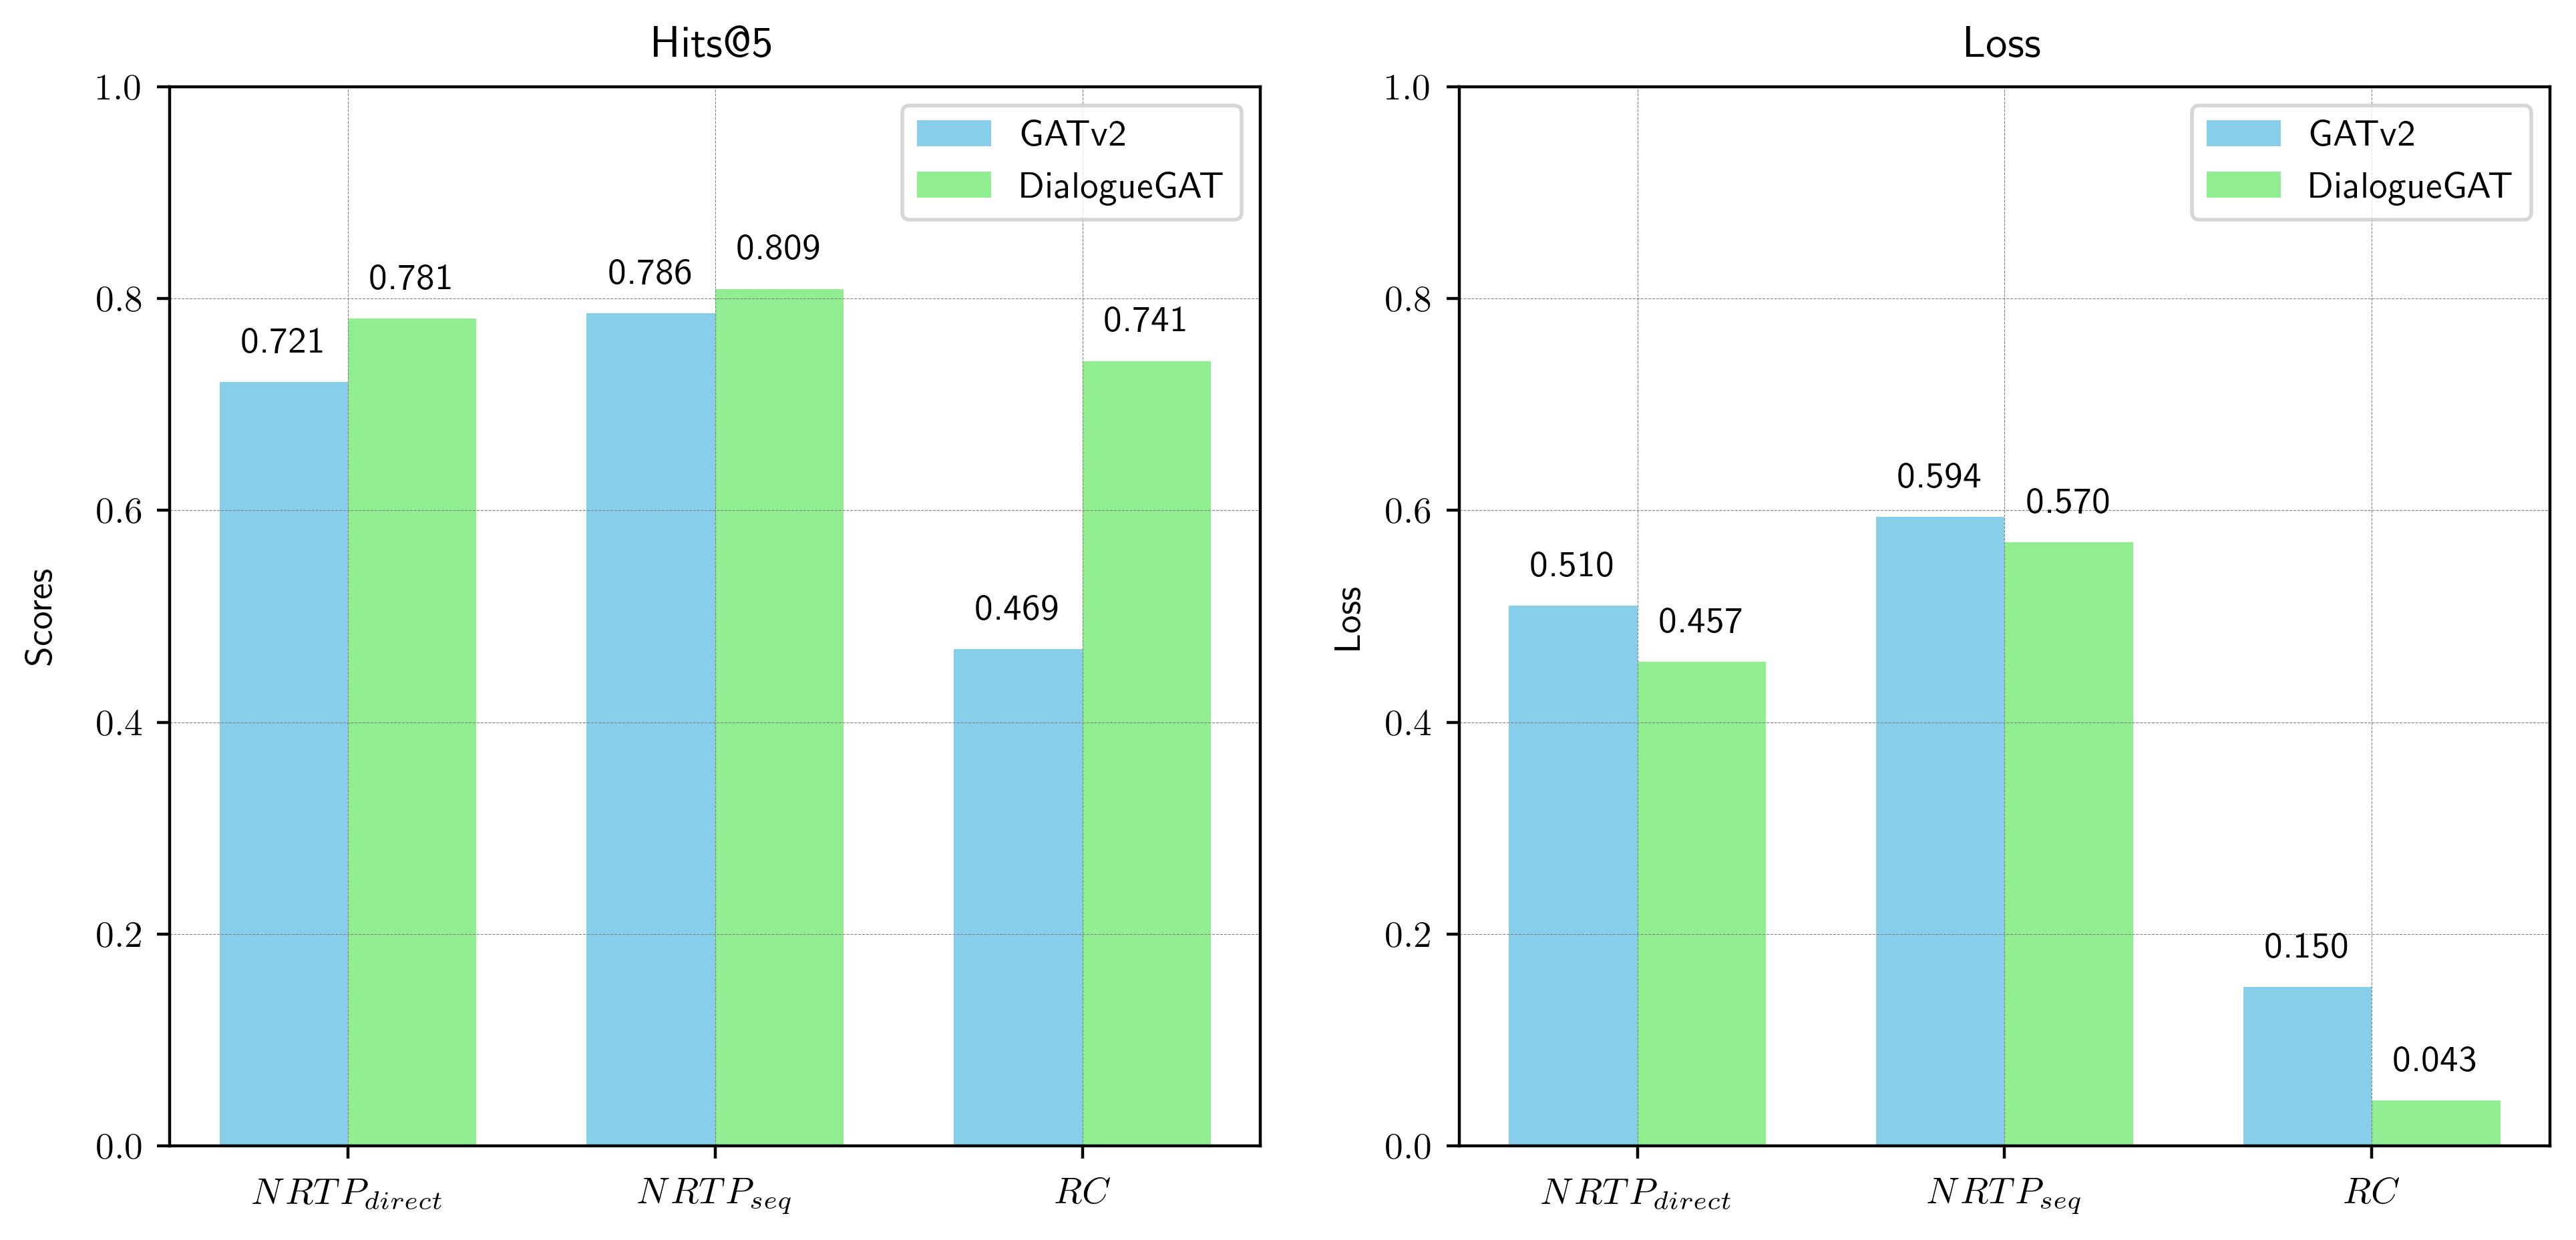
\includegraphics[width=1.0\textwidth]{./context/experiment/images/compare_gatv2_dialoguegat.png}
    \caption{Comparison of GATv2 and DialogueGAT (our proposed) as Dialogue Graph Encoders in Different Tasks. \textit{NRTP} denotes Next Response Type Prediction; \textit{RC} denotes Relations Classification.}
    \label{fig:compare_gatv2_dialoguegat}
\end{figure}

\subsection{The Effect of Dialogue Graph Encoder}
We analyze the effectiveness of the Dialogue Graph Encoder (discussed in Section 3.2.2 fine-tuning phase) under various settings. (1) \textbf{Context+Persona (Attention)}: This is our primary method where we utilize an Attention-based Feature Fusion approach to integrate representations from both the Dialogue Graph and the Persona Graph. (2) \textbf{Context+Persona (Add)}: We replace the Attention-based Feature Fusion approach with a simple addition of the persona and context representations. (3) \textbf{Context}: In this setting, we solely rely on the representation from the Dialogue Graph. (4) \textbf{Persona}: Here, we use only the representation from the Persona Graph. (5) \textbf{Random}: A random vector replaces the output of the Dialogue Graph Encoder. (6) \textbf{None}: The Dialogue Graph Encoder is completely removed from the process, allowing the generator to receive only the context and persona information from the Text Encoder. The comprehensive experimental results can be found in Figure \ref{fig:effectiveness_of_dialogue_graph_encoder}. We report the metrics for BLEU-1, ROUGE-1, and Consistency Score (C.Score).

Our experimental results demonstrate that the attention-based feature fusion approach (Context+Persona (Attention)) significantly outperforms other methods in terms of BLEU-1 and ROUGE-1 scores. These findings confirm that effectively integrating contextual and persona information through an attention mechanism enhances the similarity of the generated responses to the ground-truth responses. In contrast, simpler methods such as addition (Context+Persona (Add)) or those relying solely on context or persona information exhibit lower performance. The scores drastically decrease when random vectors are employed or when the dialogue graph encoder is omitted entirely, which emphasizes the crucial role of structured and meaningful input in producing coherent responses. The consistency scores further elucidate the models' ability to generate responses that align with persona traits. The superior performance of the attention-based method suggests its effectiveness in maintaining persona consistency within the responses. Notably, employing random vectors results in negative C.Score values, indicating that some generated responses are not only irrelevant but also contradictory to the defined personas.

These outcomes reinforce the importance of utilizing attention-based feature fusion in dialogue systems, especially in tasks that require a nuanced understanding of both context and persona. Additionally, the inferior results associated with random inputs and the complete removal of the dialogue graph encoder highlight potential risks of response incoherence and contradiction when inputs are not integrated thoughtfully. We present examples of generated results for these settings in Table \ref{table:case_study_effectiveness_of_dialogue_graph_encoder}.

\begin{figure}[H]
    \centering
    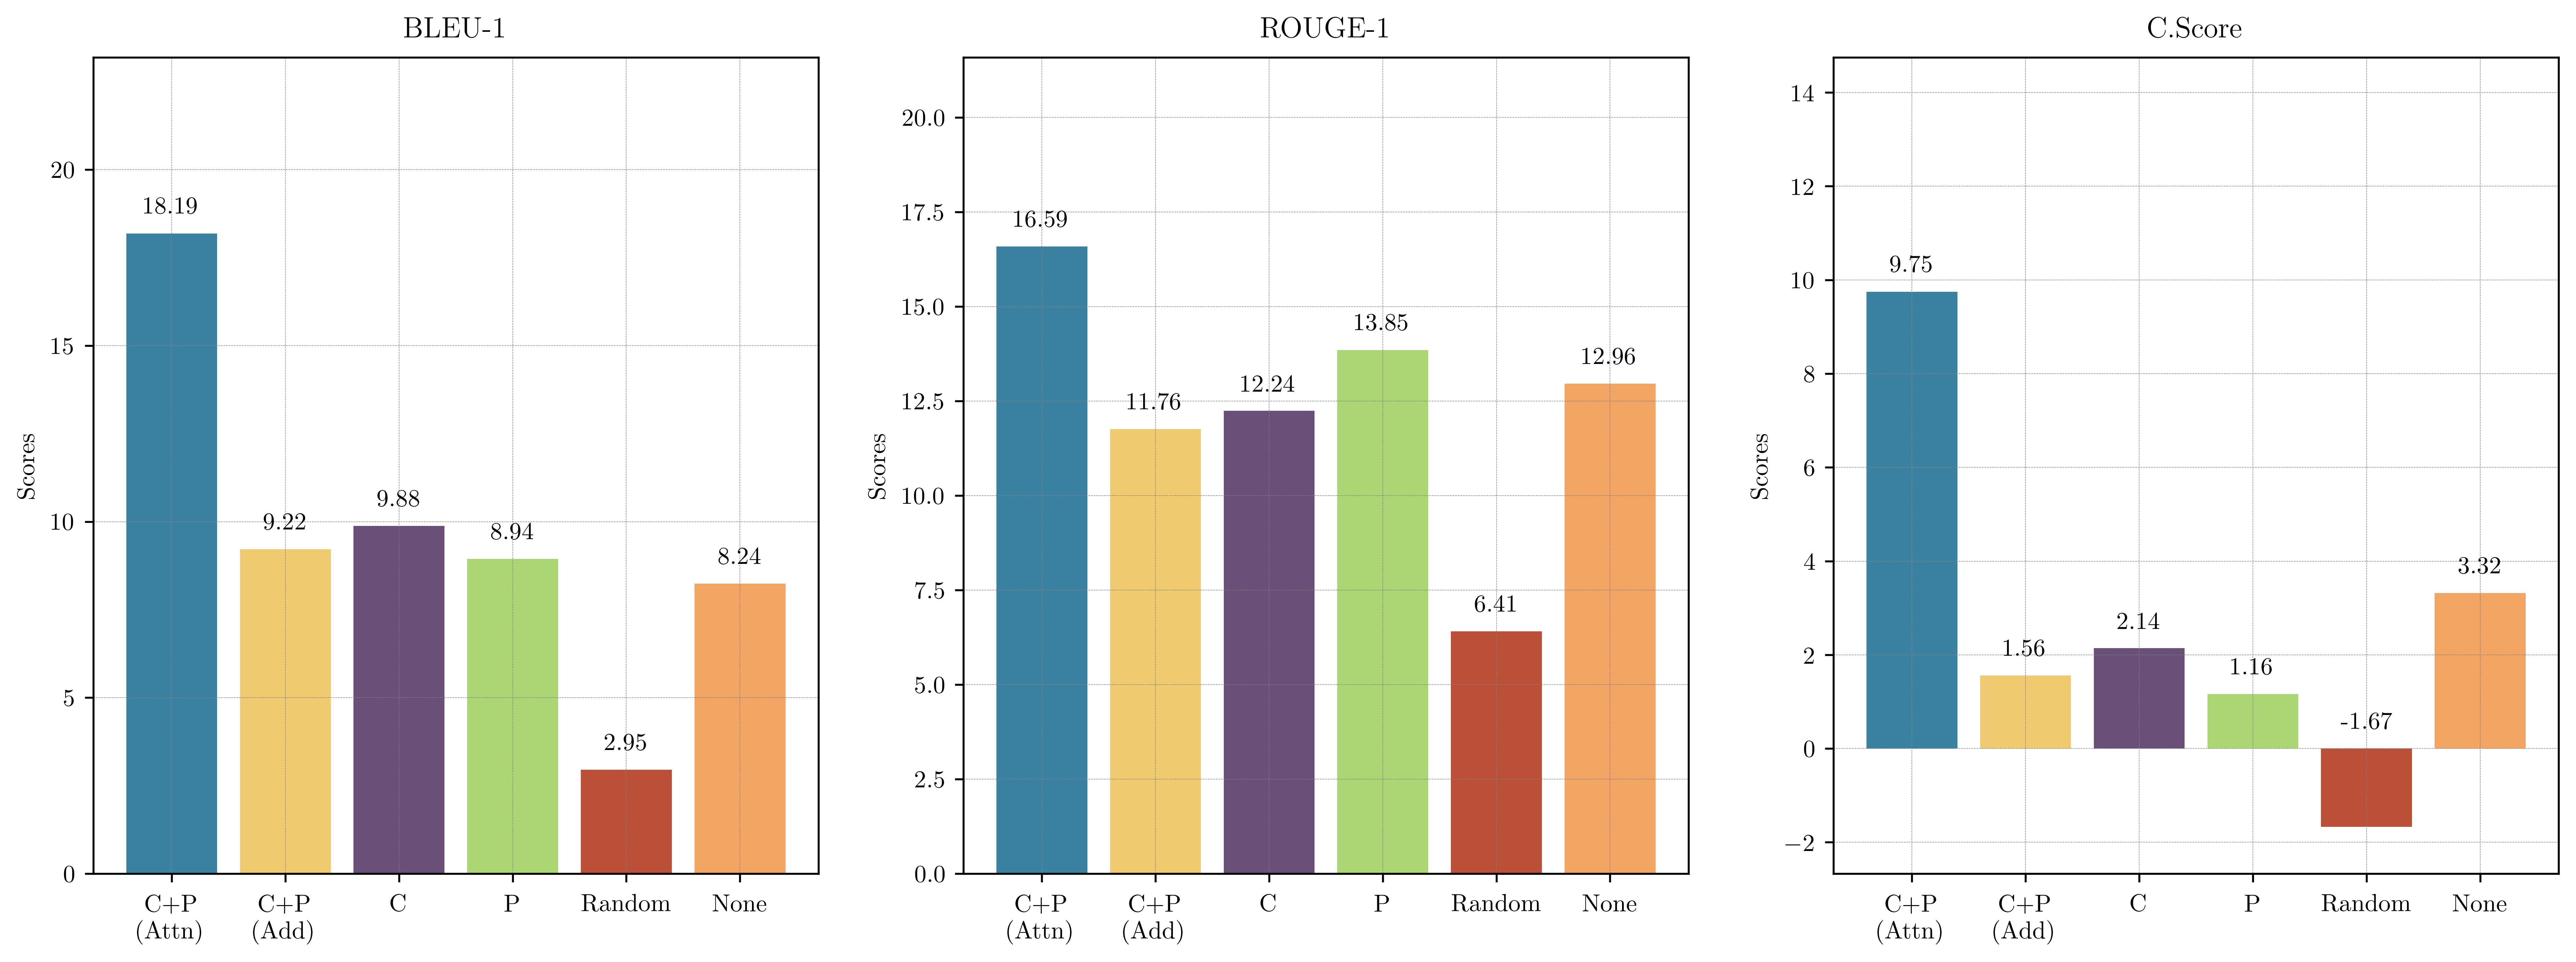
\includegraphics[width=1.0\textwidth]{./context/experiment/images/effectiveness_of_dialogue_graph_encoder.png}
    \caption{Performance analysis of Dialogue Graph Encoder across different settings. Here, "C" represents Context, and "P" represents Persona.}
    \label{fig:effectiveness_of_dialogue_graph_encoder}
\end{figure}

\subsection{The Effect of Tau Values in Dynamic Weighted Aggregation}
We analyze the effectiveness of $\tau$ in Dynamic Weighted Aggregation (discussed in Section 3.4). According to our results, shown in Figure \ref{fig:effectiveness_of_tau}, each score gradually decreases as $\tau$ increases, with the most significant drop occurring at 0.8. The metrics most noticeably affected are DEAM and C.Score, which assess coherence and personalization, respectively. Additionally, we observed that the scores, particularly for BLEU-1, actually increase when $\tau$ reaches 1.0. We hypothesize that this is due to our approach, which involves a residual connection (Eq. \ref{eq:dynamic_weighted_aggregation_output}) between the outputs of the Text Encoder and the Dialogue Graph Encoder with the results of the dynamic weighting. When $\tau$ is set to 1.0, it effectively considers only the original outputs, thus retaining a certain level of generative capability. However, this does not enhance persona-consistency and coherence as much as when $\tau$ is optimally adjusted. 

In summary, by employing Dynamic Weighted Aggregation and selecting an appropriate 
$\tau$ value, we can effectively balance coherence and personalization information, thereby generating more natural responses. This method ensures that the model not only adheres to the user-specific attributes but also maintains a logical and coherent dialogue flow, crucial for enhancing user engagement and satisfaction in interactive systems.

\begin{figure}[H]
    \centering
    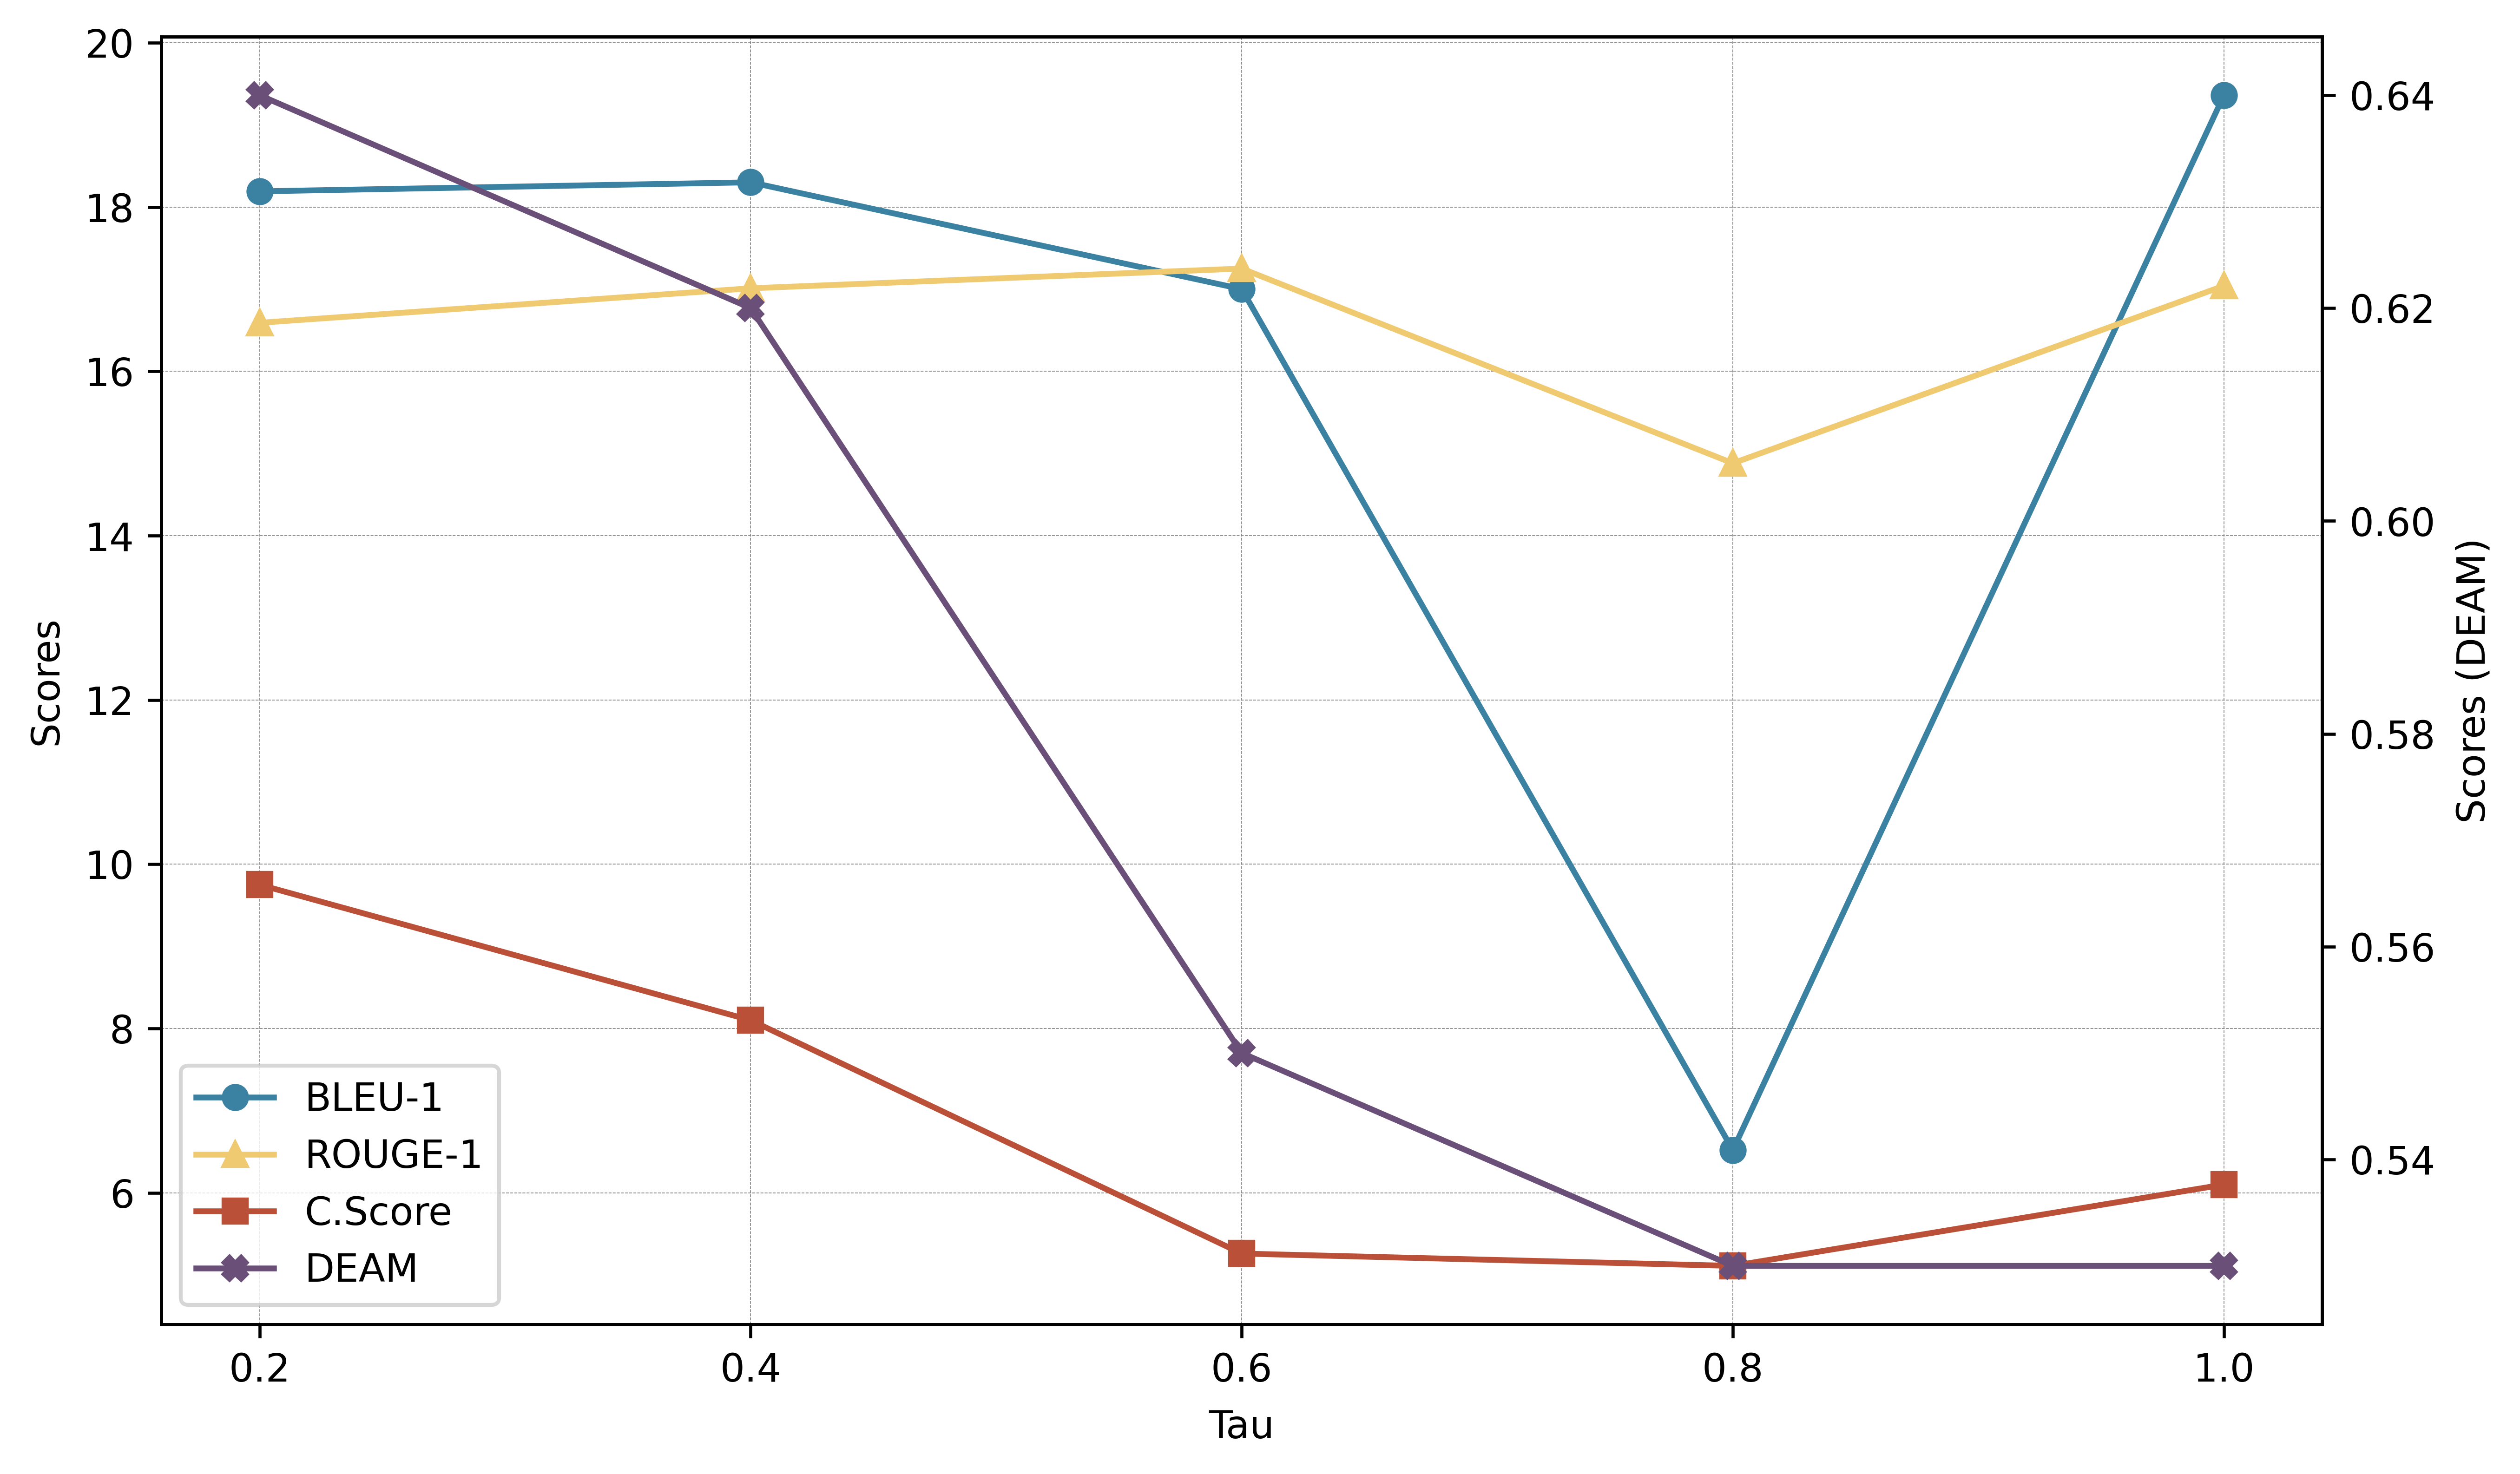
\includegraphics[width=0.9\textwidth]{./context/experiment/images/effectiveness_of_tau.png}
    \caption{Performance analysis of $\tau$ in Dynamic Weighted Aggregation.}
    \label{fig:effectiveness_of_tau}
\end{figure}

\subsection{Ablation Study}
% In our approach, to enable the dialogue graph encoder to understand the dialogue structure and adapt to subsequent coherence-related fine-tuning tasks, we designed several pre-training tasks aimed at capturing the dialogue structure. Therefore, we conducted an ablation study on these tasks to examine their impact on generating personalized responses later on. We present the results for three important metrics, coherence, personalization, and diversity, to demonstrate the impact of the pre-training task on the generated outcomes. The results of the ablation study for pre-training tasks are displayed in Table \ref{table:ablation_study}, we observed that first, after removing the Shortest Path Prediction task, the scores for coherence (QuantiDCE), persona-consistency (C.Score), and diversity (Dist-1) began to drop sharply. The goal of the Turn Classification task is to help the model capture the local structure. When this task was removed, there was a dramatic decline in scores for local coherence and persona-consistency, proving that this task aids the model in effectively capturing semantic similarities in dialogue data. Furthermore, if the Graph Reconstruction task is removed, there is a continuing downward trend in personalization scores. This confirms that our three self-supervised pretraining tasks are beneficial for the model’s understanding of dialogue structure and assist in coherence-related fine-tuning tasks, ultimately impacting the model's ability to balance coherence and persona information when generating personalized responses.

% Additionally, we conducted ablation experiments for different fine-tuning tasks. According to the conclusions drawn from Table \ref{table:ablation_study}, the removal of specific fine-tuning tasks significantly affects the model's performance metrics. Notably, the absence of tasks such as Coherence Relations Classification and Next Response Type Prediction leads to incomplete data in the table, indicating these tasks' critical roles in enhancing model accuracy and output quality. Furthermore, the removal of the Link Prediction task results in noticeable drops in both local coherence and persona consistency scores, underscoring its importance in maintaining the structural integrity and relevance of generated dialogues. These findings highlight the substantial impact that fine-tuning adjustments have on the effectiveness of the model in personalized dialogue generation.

% In our study, we investigated the impact of specific pre-training and fine-tuning tasks on the performance of a dialogue graph encoder, designed to grasp the structure of dialogues and adapt to coherence-related fine-tuning tasks. Our ablation study, summarized in Table \ref{table:ablation_study}, revealed significant declines in key performance metrics—coherence (QuantiDCE), persona-consistency (C.Score), and diversity (Dist-1)—upon the removal of these tasks. The removal of the Shortest Path Prediction (SPP) task led to sharp decreases across all metrics, underscoring its role in enhancing the encoder's capability to maintain dialogue coherence and persona consistency. Similarly, eliminating the Turn Classification (TC) task resulted in a substantial drop in local coherence and persona-consistency scores, indicating its effectiveness in capturing semantic similarities within dialogue data. Additionally, when the Graph Reconstruction (GR) task was excluded, we observed a continued decline in personalization scores, suggesting its importance in retaining a nuanced understanding of dialogue structures. Our findings were further corroborated during the fine-tuning phase, where the absence of specific tasks like Coherence Relations Classification (RC), Next Response Type Prediction (NRTP), and Link Prediction (LP) also significantly impacted model performance, particularly affecting its ability to balance coherence and personalization in generating responses. These results collectively demonstrate that both pre-training and fine-tuning tasks are crucial for optimizing the dialogue graph encoder's performance in personalized dialogue generation.

In our approach, we propose the Dialogue Graph Encoder that utilizes a two-stage training method of pretrain-finetune to allow the model to first learn dialogue structure and then further capture latent coherence relationships in dialogue data during the fine-tuning phase. To examine the impact of these diverse tasks on generating personalized responses, we conducted ablation experiments to evaluate the specific effects of removing certain pretraining and fine-tuning tasks on model performance. Experimental results summarized in Table \ref{table:ablation_study} show that when removing pre-training tasks such as Shortest Path Prediction (SPP), Turn Classification (TC), or Graph Reconstruction (GR), the model significantly decreases in key indicators like semantic consistency, persona-consistency, and diversity. Particularly, the objective of the Turn Classification (TC) task is to enable the model to predict the sequential relationship between two utterances in a dialogue, thereby learning effective utterance node representations. This aids the model's transferability to subsequent fine-tuning tasks. Hence, the removal of this task results in the largest decline in performance scores, as the model loses its capability to effectively identify local dialogue structures. These results confirm the crucial role of these pretraining tasks in helping models understand and adapt to dialogue structures, and also establish a solid foundation for subsequent supervised fine-tuning. Furthermore, ablation studies during the fine-tuning phase further emphasize the importance of tasks such as Coherence Relations Classification (RC), Next Response Type Prediction (NRTP), and Link Prediction (LP) in enhancing model performance for personalized dialogue generation. Particularly, the removal of the Coherence Relations Classification (RC) task resulted in a dramatic decrease in the model's performance in personalization assessments. This demonstrates that supervised edge-level relationship prediction tasks can aid the model in capturing potential discourse relations between adjacent nodes, learning node representations that encapsulate this information, and during subsequent Attention-based Feature Fusion, more effectively integrating utterance and persona node information for enhanced coherence and persona-consistency.

\begin{table}[ht]
    \centering
    \def\arraystretch{1.4}%
    \begin{tabular}{cccc}
    \hline
           Models & QuantiDCE & C.Score & Dist-1 \\
          \hline
          \begin{tabular}{@{}c@{}}$\textbf{MUDI}_{\text{SP}}$ \\ (ours)\end{tabular}  & 3.05 & 11.87 & 46.76 \\
          \hhline{====}
        \multicolumn{4}{c}{\textbf{Pre-training}} \\
        \hhline{====}
          \hspace*{0.65cm} w/o SPP & 2.72  & 7.05 & 34.07  \\
         \hspace*{0.5cm} w/o TC  & 2.69  & 1.18 & 33.07 \\
         \hspace*{0.5cm} w/o GR & 2.72  & 6.49 & 33.94 \\
        \hhline{====}
        \multicolumn{4}{c}{\textbf{Fine-tuning}} \\
        \hhline{====}
        \hspace*{0.5cm} w/o RC & 2.77  & 0.54 & 31.91  \\
         \hspace*{1.0cm} w/o NRTP  & 2.95  & 2.83 & 31.15 \\
         \hspace*{0.5cm} w/o LP & 2.69  & 6.22 & 34.04 \\
    \hline
    \end{tabular}
    \caption{Ablation study of the Dialogue Graph Encoder for pre-training and fine-tuning tasks.}
    \label{table:ablation_study}
\end{table}


\begin{table}[H]
\centering
\def\arraystretch{1.0}%
\begin{tabular}{|p{3.5cm}|p{12cm}|}

\hline
\rowcolor{yellow}
\multicolumn{2}{|c|}{\textbf{Persona}} \\
\hline
\multicolumn{2}{|l|}{I have two dogs.} \\
\multicolumn{2}{|l|}{I like to work on vintage cars.} \\
\multicolumn{2}{|l|}{My favorite music is country.} \\
\multicolumn{2}{|l|}{I own two vintage mustangs.} \\
\hline

\rowcolor{yellow}
\multicolumn{2}{|c|}{\textbf{Context}} \\
\hline
\multicolumn{2}{|l|}{Q: Hi! How are you doing tonight?} \\
\multicolumn{2}{|l|}{R: I'm doing great. Just relaxing with my two dogs.} \\
\multicolumn{2}{|l|}{Q: Great. In my spare time I do volunteer work.} \\
\multicolumn{2}{|l|}{R: That's neat. What kind of volunteer work do you do?} \\
\multicolumn{2}{|l|}{Q: I work in a homeless shelter in my town.} \\
\multicolumn{2}{|l|}{R: Good for you. Do you like vintage cars? I've two older mustangs.} \\
\multicolumn{2}{|l|}{Q: Cool. Not really into cars. My day job is wrestling.} \\
\multicolumn{2}{|l|}{R: Cars are my thing. Vintage cars. I love working on them. Wrestling? Do you enjoy it?} \\
\multicolumn{2}{|l|}{Q: Yes, I love the crowds, getting to know people.} \\
\multicolumn{2}{|l|}{R: I didn't think about the crowd aspect of wrestling. I do not like crowds.} \\
\multicolumn{2}{|l|}{Q: Understood. When I need to be alone, I work out a few times each week.} \\
\multicolumn{2}{|l|}{R: I agree. Working out is a great way to burn off steam. Do you like country music?} \\
\hline

\rowcolor{yellow}
\multicolumn{2}{|c|}{\textbf{Query}} \\
\hline
\multicolumn{2}{|l|}{A little bit. I can get into taylor swift.} \\

\hhline{|==|}
\rowcolor[RGB]{204,217,245}
\multicolumn{2}{|c|}{\textbf{Response}} \\
\hhline{|==|}
\textbf{Context+Persona (Attention)} & I do not like her. She's a bit too uptight for my taste. But I like her music. \\
\textbf{Context+Persona (Add)} & I can get may may and m and may and j on for more of her \\
\textbf{Context} &  What was she like? \\
\textbf{Persona} & I like country music too. \\
\textbf{Random} & you The A’ A A played The old White lead A Barbara at The The 17… \\
\textbf{None} & I like country music as well. \\

\hline
\end{tabular}
\caption{Case analysis of the effectiveness of Dialogue Graph Encoder.}
\label{table:case_study_effectiveness_of_dialogue_graph_encoder}
\end{table}

\subsection{Case Study}
Teable \ref{table:case_study_1}, \ref{table:case_study_2}, \ref{table:case_study_3}, and \ref{table:case_study_4} present the personalized responses generated by various methods using the ConvAI2 dataset. The responses generated by the proposed method, \textbf{MUDI}, demonstrated greater consistency with their respective personas and showed higher coherence with both the context and the query, appearing more human-like. As illustrated in Table \ref{table:case_study_1}, the responses from BoB were incoherent with the query, though they remained consistent with the persona. PAA often overfocused on the persona, leading to repetitive narratives of the persona description. Both LMEDR and our model produced responses that were more coherent, basing them on the user persona, but MUDI was able to generate more detailed replies, such as adding personal aspirations to the basic response about family support. 

In Table \ref{table:case_study_2}, the responses generated by BoB were irrelevant to the personas and incoherent with the context. PAA exhibited a global incoherence from the dialogue context, failing to maintain a logical flow in the conversation. While LMEDR generated a somewhat relevant response indicating a dream car, it lacked depth and personal context. On the other hand, MUDI produced a more personalized and contextually rich response that not only mentions the dream car but also integrates family dynamics, demonstrating a deeper understanding of the persona's background and the complexities in their personal relationships. 

In Table \ref{table:case_study_3}, BoB and PAA tended to overlook content from the ongoing dialogue, generating repetitive responses that rendered the entire conversation incoherent. Although LMEDR was able to generate adequate responses, our model excelled by producing more natural responses through the inclusion of responsive questions. 

As shown in Table \ref{table:case_study_4}, BoB diverged from the persona's preference by mentioning classic rock instead of country music, showing a misalignment with the user’s interests. LMEDR and PAA both correctly identified and responded with a generic appreciation for country music, aligning with the persona’s interests, yet their responses lacked specific engagement with the user’s mention of Taylor Swift or deeper personal nuances. MUDI's response, while initially not favoring Taylor Swift, cleverly circled back to acknowledge her music, demonstrating not only a nuanced understanding of the persona's tastes but also adding an interesting twist to the conversation. This illustrates MUDI's ability to generate engaging and lifelike responses, making the interaction more intriguing for users.

In summary, our model \textbf{MUDI} effectively combines dialogue and persona elements to generate appropriate responses. Furthermore, it excels at using responsive questions to enhance the conversation's naturalness.


% ----------------------------------------------
% Case Study 1
% ----------------------------------------------

\begin{table}[ht]
\centering
\def\arraystretch{1.6}%
\begin{tabular}{|l|p{11cm}|}

\hline
\rowcolor{yellow}
\multicolumn{2}{|c|}{\textbf{Persona}} \\
\hline
\multicolumn{2}{|l|}{My dream car is a rolls royce ghost.} \\
\multicolumn{2}{|l|}{I currently work for a watch dealer.} \\
\multicolumn{2}{|l|}{My family does not support my career choices.} \\
\multicolumn{2}{|l|}{I often shop for shoes and watches.} \\
\multicolumn{2}{|l|}{I like shopping.} \\
\hline

\rowcolor{yellow}
\multicolumn{2}{|c|}{\textbf{Context}} \\
\hline
\multicolumn{2}{|l|}{Q: Good evening. What are you up to?} \\
\multicolumn{2}{|l|}{R: Hello, how are you ? I am well. I like to shop for shoes and watches.} \\
\multicolumn{2}{|l|}{Q: I don't shop much. Prefer to relax at home with my cow.} \\
\multicolumn{2}{|l|}{R: What do you do ? I'm work for a watch dealer.} \\
\hline

\rowcolor{yellow}
\multicolumn{2}{|c|}{\textbf{Query}} \\
\hline
\multicolumn{2}{|l|}{No wonder you like watches ! I'm a commercial electrician.} \\

\hhline{|==|}
\rowcolor[RGB]{204,217,245}
\multicolumn{2}{|c|}{\textbf{Response}} \\
\hhline{|==|}
\textbf{GOLD} & wonderful! yeah, however, my family does not support my choice of career. \\
\textbf{BoB} & I work at a dealership, but I am not very good at it. \\
% \textbf{P$^2$BOT} & what do you do for a living ? i work for the watch. \\
\textbf{LMEDR} & My family does not support my career choices. \\
\textbf{PAA} & I like to shop. I also like to shop. \\
\textbf{MUDI} & My family does not support my career choices. I want to drive a rolls royce ghost. \\

\hline
\end{tabular}
\caption{Case analysis of personalized response generation on the ConvAI2 dataset.}
\label{table:case_study_1}
\end{table}

% ----------------------------------------------
% Case Study 2
% ----------------------------------------------

\begin{table}[ht]
\centering
\def\arraystretch{1.6}%
\begin{tabular}{|l|p{11cm}|}

\hline
\rowcolor{yellow}
\multicolumn{2}{|c|}{\textbf{Persona}} \\
\hline
\multicolumn{2}{|l|}{My dream car is a rolls royce ghost.} \\
\multicolumn{2}{|l|}{I currently work for a watch dealer.} \\
\multicolumn{2}{|l|}{My family does not support my career choices.} \\
\multicolumn{2}{|l|}{I often shop for shoes and watches.} \\
\multicolumn{2}{|l|}{I like shopping.} \\
\hline

\rowcolor{yellow}
\multicolumn{2}{|c|}{\textbf{Context}} \\
\hline
\multicolumn{2}{|l|}{Q: Good evening. What are you up to?} \\
\multicolumn{2}{|l|}{R: Hello, how are you ? I am well. I like to shop for shoes and watches.} \\
\multicolumn{2}{|l|}{Q: I don't shop much. Prefer to relax at home with my cow.} \\
\multicolumn{2}{|l|}{R: What do you do ? I'm work for a watch dealer.} \\
\multicolumn{2}{|l|}{Q: No wonder you like watches! I'm a commercial electrician.} \\
\multicolumn{2}{|l|}{R: Wonderful! Yeah, however, my family does not support my choice of career.} \\
\hline

\rowcolor{yellow}
\multicolumn{2}{|c|}{\textbf{Query}} \\
\hline
\multicolumn{2}{|l|}{Why not? Family is important.} \\

\hhline{|==|}
\rowcolor[RGB]{204,217,245}
\multicolumn{2}{|c|}{\textbf{Response}} \\
\hhline{|==|}
\textbf{GOLD} & I'm not sure why they do not. Do you like cars? \\
\textbf{BoB} & I am not sure. I am a watch dealer. \\
% \textbf{P$^2$BOT} & my family doesn't support my lifestyle choices. \\
\textbf{LMEDR} & I do not know. I do have a dream car though. It is a rolls royce ghost. \\
\textbf{PAA} & I am a watch dealer. I have a lot of money. \\
\textbf{MUDI} & yes agree! I want to drive a rolls royce ghost car, but my family does not like that. \\

\hline
\end{tabular}
\caption{Case analysis of personalized response generation on the ConvAI2 dataset.}
\label{table:case_study_2}
\end{table}

% ----------------------------------------------
% Case Study 3
% ----------------------------------------------

\begin{table}[ht]
\centering
\def\arraystretch{1.6}%
\begin{tabular}{|l|p{11cm}|}

\hline
\rowcolor{yellow}
\multicolumn{2}{|c|}{\textbf{Persona}} \\
\hline
\multicolumn{2}{|l|}{I listen to rap music.} \\
\multicolumn{2}{|l|}{I produce music for artists.} \\
\multicolumn{2}{|l|}{I drive a 2015 Honda Civic.} \\
\multicolumn{2}{|l|}{My favorite food is pizza.} \\
\hline

\rowcolor{yellow}
\multicolumn{2}{|c|}{\textbf{Context}} \\
\hline
\multicolumn{2}{|l|}{Q: Hi, how are you? Do you have any brothers or sisters?} \\
\multicolumn{2}{|l|}{R: No I don't do you?} \\
\multicolumn{2}{|l|}{Q: Yes, I'm 13 and I've an older brother.} \\
\multicolumn{2}{|l|}{R: That's nice what kind of music do you like.} \\
\multicolumn{2}{|l|}{Q: I do not have much time as I play soccer. You?} \\
\multicolumn{2}{|l|}{R: I am a music producer for rap artists} \\
\hline

\rowcolor{yellow}
\multicolumn{2}{|c|}{\textbf{Query}} \\
\hline
\multicolumn{2}{|l|}{Cool I like rap. I hate maths though! Do you have other hobbies?} \\

\hhline{|==|}
\rowcolor[RGB]{204,217,245}
\multicolumn{2}{|c|}{\textbf{Response}} \\
\hhline{|==|}
\textbf{GOLD} & Work takes up a lot of my time. \\
\textbf{BoB} & I like music and I like to listen to music. \\
% \textbf{P$^2$BOT} & I like to listen to rap music. \\
\textbf{LMEDR} & I like to drive my honda civic. \\
\textbf{PAA} & I like rap music, I produce it for artists. \\
\textbf{MUDI} & I like to go my old Honda Civic car and eat pizza. Do you have any hobbies? \\

\hline
\end{tabular}
\caption{Case analysis of personalized response generation on the ConvAI2 dataset.}
\label{table:case_study_3}
\end{table}

% ----------------------------------------------
% Case Study 4
% ----------------------------------------------

\begin{table}[ht]
\centering
\def\arraystretch{1.6}%
\begin{tabular}{|l|p{11cm}|}

\hline
\rowcolor{yellow}
\multicolumn{2}{|c|}{\textbf{Persona}} \\
\hline
\multicolumn{2}{|l|}{I have two dogs.} \\
\multicolumn{2}{|l|}{I like to work on vintage cars.} \\
\multicolumn{2}{|l|}{My favorite music is country.} \\
\multicolumn{2}{|l|}{I own two vintage mustangs.} \\
\hline

\rowcolor{yellow}
\multicolumn{2}{|c|}{\textbf{Context}} \\
\hline
\multicolumn{2}{|l|}{Q: Hi! How are you doing tonight?} \\
\multicolumn{2}{|l|}{R: I'm doing great. Just relaxing with my two dogs.} \\
\multicolumn{2}{|l|}{Q: Great. In my spare time I do volunteer work.} \\
\multicolumn{2}{|l|}{R: That's neat. What kind of volunteer work do you do?} \\
\multicolumn{2}{|l|}{Q: I work in a homeless shelter in my town.} \\
\multicolumn{2}{|l|}{R: Good for you. Do you like vintage cars? I've two older mustangs.} \\
\multicolumn{2}{|l|}{Q: Cool. Not really into cars. My day job is wrestling.} \\
\multicolumn{2}{|l|}{R: Cars are my thing. Vintage cars. I love working on them. Wrestling? Do you enjoy it?} \\
\multicolumn{2}{|l|}{Q: Yes, I love the crowds, getting to know people.} \\
\multicolumn{2}{|l|}{R: I didn't think about the crowd aspect of wrestling. I do not like crowds.} \\
\multicolumn{2}{|l|}{Q: Understood. When I need to be alone, I work out a few times each week.} \\
\multicolumn{2}{|l|}{R: I agree. Working out is a great way to burn off steam. Do you like country music?} \\
\hline

\rowcolor{yellow}
\multicolumn{2}{|c|}{\textbf{Query}} \\
\hline
\multicolumn{2}{|l|}{A little bit. I can get into taylor swift.} \\

\hhline{|==|}
\rowcolor[RGB]{204,217,245}
\multicolumn{2}{|c|}{\textbf{Response}} \\
\hhline{|==|}
\textbf{GOLD} & lol. She's more pop now. Her old stuff was country. I like classic country. \\
\textbf{BoB} & I'm not much into music. I like classic rock. \\
% \textbf{P$^2$BOT} &  \\
\textbf{LMEDR} & Yes, I love country music. \\
\textbf{PAA} & I do. I love to listen to country music. \\
\textbf{MUDI} & I do not like her. She's a bit too uptight for my taste. But I like her music. \\

\hline
\end{tabular}
\caption{Case analysis of personalized response generation on the ConvAI2 dataset.}
\label{table:case_study_4}
\end{table}

% ------------------------------------------------
\EndChapter
% ------------------------------------------------


% Conclusion chapter
% ------------------------------------------------
\StartChapter{Conclusion}{chapter:conclusion}
% ------------------------------------------------
In this work, we propose a new method, \textbf{MUDI}, to effectively model discourse relations in personalized dialogue generation. To the best of our knowledge, \textbf{MUDI} is the first framework to jointly integrate Discourse Relations and Persona in Personalized Dialogue. Firstly, we propose DialogueGAT, a dialogue-enhanced GNN, as a Dialogue Graph Encoder, designed to capture dialogue structure and contextual discourse relations. Additionally, we utilize an Attention-Based Feature Fusion method to effectively integrate context relations and persona information. We further enhance our model by employing a Text Encoder to capture persona-aware dialogue representations. We increase the decoder's ability to consider coherent information while predicting the next token by leveraging both a prompt-based conditional dialogue generation mechanism, which uses prompts to guide the response generation process, and our coherence-aware attention mechanism, which incorporates learnable embeddings and token representations. Finally, we leverage Dynamic Weighting Aggregation to balance the information between coherence-aware and persona-aware dialogue representations, ensuring a robust integration of both elements.

Extensive experiments and analyses demonstrate that our method, \textbf{MUDI}, significantly improves the quality of personalized responses by making them more coherent, informative, and aligned with the user's persona traits, as well as more human-like.

% ------------------------------------------------
\EndChapter
% ------------------------------------------------


% Future work chapter
%\input{./context/future-work/future-work}

% ------------------------------------------------

% 參考文獻 References
% References and bibliography

% Import the files that contain your references.
% If you set some references file,
% you need to use at least one cite to make Latex work.

\ReferencesFiles{./thesis/context/references/paper}{./thesis/context/references/misc}{./thesis/context/references/book}

% ------------------------------------------------

% 附錄 Appendix
%% ------------------------------------------------
\StartAppendix
% ------------------------------------------------

\input{./example/appendix/acceptable-dept}
\input{./example/appendix/submit-flow}
\input{./example/appendix/thesis-spec}
\input{./example/appendix/e-paper_upload}
\input{./example/appendix/e-paper_upload_ppt}
\input{./example/appendix/oral-notice}
\input{./example/appendix/faq}
\input{./example/appendix/unicode-symbols}

% ------------------------------------------------
\EndAppendix
% ------------------------------------------------


% ------------------------------------------------
}%
  {% ------------------------------------------------
%
%論文內容次序:
% 1.考試合格證明
% 2.中英文摘要(論文以中文撰寫者須附英文延伸摘要)
% 3.誌謝
% 4.目錄
% 5.表目錄
% 6.圖目錄
% 7.符號
% 8.主文
% 9.參考文獻
% 10.附錄
%
% 註: 參考文獻書寫注意事項:
% (1).
%    文學院之中文文獻依分類及年代順序排列。
%    其他學院所之文獻依英文姓氏第一個字母
%    (或中文姓氏第一個字筆劃)及年代順序排列。
%
% (2).
%    期刊文獻之書寫依序為:
%        姓名、文章名稱、期刊名、卷別、期別、頁別、年代。
%
% (3).
%    書寫之文獻依序為:
%        姓名、書名、出版商名、出版地、頁別、年代。
%
% ------------------------------------------------

% 封面內頁 Inner Cover
%
% 封面: 顯示所有封面內容, 沒有學校Logo
%     主要用在印刷版, 如精裝版 或 平裝版
%     (使用cover.tex來產生)
%
% 內頁: 顯示所有封面內容, 沒有學校Logo
%     主要用在電子版 + 印刷版
%
% 只要是印刷版, 不論是精裝版或平裝版, 都是 封面 (殼/皮) + 內頁.
% 只有在電子版時, 第一頁就是封面內頁.

\DisplayInnerCover

% ------------------------------------------------

% 學位考試論文證明書
\DisplayOral

% ------------------------------------------------

% 摘要 Abstract
% 除了外籍生, 本地生和僑生都是要編寫中文和英文摘要
% 論文以中文撰寫須以英文補寫 800 至 1200 字數的英文延伸摘要 (Extended Abstract)
% 詳細可看附件的學校要求或看example中的英文延伸摘要

% ------------------------------------------------
\StartAbstractChi
% ------------------------------------------------

這是國立成功大學碩博士用畢業論文的LaTex模版. 這模版是使用學校最新的畢業論文要求來設計(參考: 附錄 - 撰寫論文須知 P.\RefPage{appendix:thesis-spec}).

這模版的目標是為了提供學生可以使用LaTex來寫畢業論文. 但是各系所有各自的格式, 故請在使用前先留意自己的系所有沒有格式要求 (參考: 附錄 - 可使用的系所 P.\RefPage{appendix:acceptable-dept}). 如果沒有, 則這模版應該用來使用; 否則要看系所上的格式, 是否跟這模版有相同的寫法.

這模版的內容是我參考了我所拿到的一些畢業論文的LaTex模版設計, 跟系上老師的一些對話, 和上課所聽得出的結論和想法而寫出的, 所以某些地方會帶有我們濃郁的資工系味道. 另外如果有任何的老師 (不論本系外系)可以提供一些意見或想法的話, 我會十分感謝的.

這模版盡量以全自動化方式去處理一些不用你去煩惱的部份, 如排版和設計. 只留下要你去填寫的部份, 所以只要選擇和填入你的內容, 就能得到一份符合學校要求的畢業論文.

最後, 希望你使用愉快.

% ------------------------------------------------
% 如果在conf.tex中的\SetAbstractChiKeywords有設定任何的關鍵字,
% 那中文版的關鍵字會在使用\EndAbstractChi後同時顯示出來.
\EndAbstractChi
% ------------------------------------------------
             % 中文版
% ------------------------------------------------
\StartAbstract
% ------------------------------------------------
In dialogue generation, the naturalness of responses is key for effective human-machine interaction, significantly enhancing user experience. Personalized dialogue generation poses even greater challenges, as the responses must be coherent and consistent with the user's personal traits or persona descriptions. In this study, we propose a novel method named \textbf{MUDI} (\textbf{Mu}ltiple \textbf{Di}scourse Relations Graph Learning) aimed at effectively modeling and integrating discourse relations and persona information within the context of personalized dialogue generation. We initially utilize Large Language Models to assist in annotating discourse relations and to transform dialogue data into structured dialogue graphs. We employ our newly proposed DialogueGAT as the graph encoder, which captures implicit discourse relations within this structure. Persona descriptions are also encoded into fully-connected persona graphs, facilitating the capture of semantic relationships between persona elements. An Attention-Based Feature Fusion method integrates data from both graphs, creating a personalized, coherence-aware dialogue representation. In the personalized response generation phase, a Prompt-based mechanism and a Coherence-Aware Attention strategy are implemented to enhance the decoder's consideration of discourse relations. Our experiments and case studies demonstrate significant improvements in the quality of personalized responses, making them more coherent, aligned with persona, and natural, thus resembling human-like dialogue exchanges.

% In dialogue generation, high naturalness of responses is crucial for effective human-machine interaction, significantly enhancing user experience. Personalized response generation poses even greater challenges, as the responses must be coherent and consistent with the user's personal traits or persona descriptions. In this study, we propose a novel method named \textbf{MUDI} (\textbf{Mu}ltiple \textbf{Di}scourse Relations Graph Learning) aimed at effectively modeling and integrating discourse relations and persona information within the context of personalized dialogue generation. Initially, to enable the model to learn discourse coherence relations within dialogues, we utilize Large Language Models to assist in annotating discourse relations in the dialogue data. Inspired by prior research, we transform the dialogue data into a dialogue graph, then apply our proposed DialogueGAT as an encoder to capture the implicit discourse coherence relations within the dialogue structure. Additionally, we transform persona descriptions into fully-connected persona graphs through the graph encoder to capture semantic relationships between persona sentences. Finally, we employ an attention mechanism-based feature fusion method to integrate information from both the dialogue and persona graphs, creating a personalized, coherence-aware dialogue representation. We also capture the implicit relationships between dialogue context and persona descriptions at the semantic and paragraph levels through a text encoder. In the response generation phase, we first employ a prompt-based conditional dialogue generation mechanism, using carefully designed prompts to guide the generation of personalized responses. We introduce a coherence-enhanced attention mechanism, combining learnable embeddings and text representations to enhance the decoder's ability to consider discourse relations when predicting the next word, allowing it to consider vocabulary that carries implicit coherence information during text generation. Experimental results and case studies demonstrate that our method significantly improves the quality of personalized dialogue responses, effectively integrating discourse relations and persona information, making the responses more coherent, adhering to persona settings, and more natural, resembling human-like dialogue responses.

% ------------------------------------------------
\EndAbstract
% ------------------------------------------------
             % 英文版
%% ------------------------------------------------
\StartExtendedAbstract
% ------------------------------------------------

\ExtAbstractSummary{%
The summary is a short, informative abstract of no more than 250 words. References should not be cited. The summary should (1) state the scope and objectives of the research, (2) describe the methods used, (3) summarize the results, and (4) state the principal conclusions. Text of the summary should be 12 pt Times New Roman font, single-spaced and justified. A single line space should be left below the title `SUMMARY'. Leave a single line space above the key words listed below.
} % End of \ExtAbstractSummary{}

% ------------------------------------------------

\ExtAbstractChapter{INTRODUCTION}
The purpose of the introduction is to tell readers why they should want to read your thesis/ dissertation. This section should provide sufficient background information to allow readers to understand and evaluate the paper's results.

The introduction should (1) present the nature and scope of the problem, (2) review related literature, (3) describe the materials used and method(s) of the study, and (4) describe the main results of the study.

All text in the main body of the extended abstract should be 12 pt Times New Roman font, single-spaced and justified. Main headings are placed in the centre of the column, in capital letters using 12 pt Times New Roman Bold font. Subheadings are placed on the left margin of the column and are typed in 12 pt Times New Roman Bold font.

% ------------------------------------------------

\ExtAbstractChapter{MATERIALS AND METHODS}
There is flexibility as to the naming of the section (or sections) that provide information on the method(s) or theories employed. The methodology employed inthe work must be described in sufficient detail or with sufficient references so that the results could be duplicated.

Your materials should be organised carefully. Include all the data necessary to support your conclusions, but exclude redundant or unnecessary data.

% ------------------------------------------------

\ExtAbstractChapter{RESULTS AND DISCUSSION}
The results and discussion sections present your research findings and your analysis of those findings. The results of experiments can be presented as tables or figures.

% ------------------------------------------------

\ExtAbstractSection{Figures and Tables}
Figures may be integrated within the results section of the extended abstract, or they can be appended to the end of the written text. Figures should be black \& white. They should be no wider than the width of the A4 page.

Tables can be created within Word. As noted for figures above, if a table is to be placed within the text, it can be no wider than the width of the A4 page. Larger tables will need to be placed at the end of the abstract.

Figures and tables should be numbered according to the order they are referenced in the paper. Figures and tables should be referred to by their number in the text. When referring to figures and tables in the text, spell out and capitalize the word Figure or Table. All figures and tables must have captions.

% ------------------------------------------------

\ExtAbstractSection{Captions}
Captions should clearly explain the significance of the figure or table without reference to the text. Details in captions should not be restated in the text. Parameters in figure captions should be included and presented in words rather than symbols.

Captions should be placed directly above the relevant table and beneath the relevant figure. The caption should be typed in 12 pt Times New Roman Bold font. Spell out the word `Table' or `Figure' in full. An example table and a figure follow.

% ------------------------------------------------

\InsertTable
  [caption={Specifications of the engine}]
  {
    \begin{tabular}{llll}
    \hline
    Engine &  &  & OPEL Astra C16SE \\ \hline
    Displacement (cc) &  &  & 1598 \\
    Bore x stroke(mm x mm) &  &  & 79 x 81.5 \\
    Value mechanism &  &  & SOHC \\
    Number of valves &  &  & Intake 4, exhaust 4 \\
    Compression ratio &  &  & 9.8:1 \\
    Torque &  &  & 135/3400 Nm/rpm \\
    Power &  &  & 74/5800 kW/rpm \\
    Ignition sequence &  &  & 1-3-4-2 \\
    Spark plug &  &  & BPR6ES \\
    Fuel &  &  & 95 unleaded gasoline \\
    Cylinder arrangment &  &  & In-line 4 cylinders \\ \hline
    \end{tabular}
  } % End of  \InsertTable{}

\InsertFigure
  [scale=0.5,
    caption={HC emission as a function of equivalence ratio}]
  {./example/abstract/pic/extended-abstract-2.jpg}

% ------------------------------------------------

\ExtAbstractChapter{CONCLUSION}
This section should include (1) the main points of your paper and why they are significant, (2) any exceptions to, problems with, or limitations to your argument, (3) agreements or disagreements with previously published work, (4) theoretical and practical implications of the work, and (5) conclusions drawn.

% ------------------------------------------------
\EndExtendedAbstract
% ------------------------------------------------
        % 英文延伸摘要

% ------------------------------------------------

% 誌謝 Acknowledgments
% 誌謝正常應該只要寫一種版本就可,
% 提供2種以自行選擇所顯示的語言.
% 2種同時編寫都是可以的.

% ------------------------------------------------
\StartAbstractChi
% ------------------------------------------------

這是國立成功大學碩博士用畢業論文的LaTex模版. 這模版是使用學校最新的畢業論文要求來設計(參考: 附錄 - 撰寫論文須知 P.\RefPage{appendix:thesis-spec}).

這模版的目標是為了提供學生可以使用LaTex來寫畢業論文. 但是各系所有各自的格式, 故請在使用前先留意自己的系所有沒有格式要求 (參考: 附錄 - 可使用的系所 P.\RefPage{appendix:acceptable-dept}). 如果沒有, 則這模版應該用來使用; 否則要看系所上的格式, 是否跟這模版有相同的寫法.

這模版的內容是我參考了我所拿到的一些畢業論文的LaTex模版設計, 跟系上老師的一些對話, 和上課所聽得出的結論和想法而寫出的, 所以某些地方會帶有我們濃郁的資工系味道. 另外如果有任何的老師 (不論本系外系)可以提供一些意見或想法的話, 我會十分感謝的.

這模版盡量以全自動化方式去處理一些不用你去煩惱的部份, 如排版和設計. 只留下要你去填寫的部份, 所以只要選擇和填入你的內容, 就能得到一份符合學校要求的畢業論文.

最後, 希望你使用愉快.

% ------------------------------------------------
% 如果在conf.tex中的\SetAbstractChiKeywords有設定任何的關鍵字,
% 那中文版的關鍵字會在使用\EndAbstractChi後同時顯示出來.
\EndAbstractChi
% ------------------------------------------------
             % 中文版
%% ------------------------------------------------
\StartAbstract
% ------------------------------------------------
In dialogue generation, the naturalness of responses is key for effective human-machine interaction, significantly enhancing user experience. Personalized dialogue generation poses even greater challenges, as the responses must be coherent and consistent with the user's personal traits or persona descriptions. In this study, we propose a novel method named \textbf{MUDI} (\textbf{Mu}ltiple \textbf{Di}scourse Relations Graph Learning) aimed at effectively modeling and integrating discourse relations and persona information within the context of personalized dialogue generation. We initially utilize Large Language Models to assist in annotating discourse relations and to transform dialogue data into structured dialogue graphs. We employ our newly proposed DialogueGAT as the graph encoder, which captures implicit discourse relations within this structure. Persona descriptions are also encoded into fully-connected persona graphs, facilitating the capture of semantic relationships between persona elements. An Attention-Based Feature Fusion method integrates data from both graphs, creating a personalized, coherence-aware dialogue representation. In the personalized response generation phase, a Prompt-based mechanism and a Coherence-Aware Attention strategy are implemented to enhance the decoder's consideration of discourse relations. Our experiments and case studies demonstrate significant improvements in the quality of personalized responses, making them more coherent, aligned with persona, and natural, thus resembling human-like dialogue exchanges.

% In dialogue generation, high naturalness of responses is crucial for effective human-machine interaction, significantly enhancing user experience. Personalized response generation poses even greater challenges, as the responses must be coherent and consistent with the user's personal traits or persona descriptions. In this study, we propose a novel method named \textbf{MUDI} (\textbf{Mu}ltiple \textbf{Di}scourse Relations Graph Learning) aimed at effectively modeling and integrating discourse relations and persona information within the context of personalized dialogue generation. Initially, to enable the model to learn discourse coherence relations within dialogues, we utilize Large Language Models to assist in annotating discourse relations in the dialogue data. Inspired by prior research, we transform the dialogue data into a dialogue graph, then apply our proposed DialogueGAT as an encoder to capture the implicit discourse coherence relations within the dialogue structure. Additionally, we transform persona descriptions into fully-connected persona graphs through the graph encoder to capture semantic relationships between persona sentences. Finally, we employ an attention mechanism-based feature fusion method to integrate information from both the dialogue and persona graphs, creating a personalized, coherence-aware dialogue representation. We also capture the implicit relationships between dialogue context and persona descriptions at the semantic and paragraph levels through a text encoder. In the response generation phase, we first employ a prompt-based conditional dialogue generation mechanism, using carefully designed prompts to guide the generation of personalized responses. We introduce a coherence-enhanced attention mechanism, combining learnable embeddings and text representations to enhance the decoder's ability to consider discourse relations when predicting the next word, allowing it to consider vocabulary that carries implicit coherence information during text generation. Experimental results and case studies demonstrate that our method significantly improves the quality of personalized dialogue responses, effectively integrating discourse relations and persona information, making the responses more coherent, adhering to persona settings, and more natural, resembling human-like dialogue responses.

% ------------------------------------------------
\EndAbstract
% ------------------------------------------------
             % 英文版

% ------------------------------------------------

% 目錄 (內容, 圖表和圖片) Index of contents, tables and figures.
% 內容會自動產生 The indices will generate in automate.
\DisplayIndex                 % 顯示索引
\DisplayTablesIndex   % 顯示表格索引
\DisplayFiguresIndex  % 顯示圖片索引

% ------------------------------------------------

% Nomenclature
% % ------------------------------------------------
\StartSection{術語/符號 Nomenclature}{chapter:how-to:write:nomenclature}
% ------------------------------------------------

Nomenclature在定義一些在整份論文中所會用到的變數是很常用到的. 它的位置會出現在文章當中或是在Chapter 1之前. 它的設計沒有一個標準答案, 在不同的情況下可能有不同顯示方式, 但它基本上跟一張Table是沒差的. 而它在Latex中是使用一個package名為`nomencl'.

但經過研究了一下package `nomencl'或tabbing這些用來建Nomenclature的方式後, 發現`nomencl'在設計上反而會增加在產生論文時的步驟; 而tabbing要自行定義一個闊度才能弄得比較好看, 但同時內容卻出現沒法置中和設計上等一些問題. 故最後決定直接套用Table來讓同學更能自由的設計不同的Nomenclature table.

設計Nomenclature table需要2個知識或工具:\\
1) 設計一張Table, 這邊請參考P. \RefPage{chapter:how-to:write:table}.\\
2) 有關所需要用到的符號, 請參考Equation (P. \RefPage{chapter:how-to:write:equation})中所使用到的工具, Texmarker左邊的工具列, 或看這幾個網頁\RefBib{web:symbols:site1}\RefBib{web:symbols:site2}\RefBib{web:symbols:site3}, 應該已經足夠同學們寫出合適的符號.

% ------------------------------------------------
%\newpage
\StartSubSection{使用方式}

如果是指是在Chapter 1之前的一大張的Nomenclature table, 為Nomenclature Chapter.
  \begin{verbatim}
  \StartNomChapter{ NAME }{ LABEL }
  \EndNomChapter
  \end{verbatim}
Nomenclature Chapter跟一般Chapter的使用方式是一樣的, 但差別在於不會出現`Chapter'這字眼. 而由於大家的Nomenclature Chapter name可能不一樣, 故跟Chapter一樣可設定自行的name.

而如果是在文章當中的Nomenclature table. 基本上就是使用同一個的`\verb|\InsertTable|', 但還可以使用`nomtitle'來設定標題. `nomtitle'跟`caption'的差別是, 使用`nomtitle'所顯示出來的標題是沒有`Table XX:'為開頭, 同樣都是使用`pos'來控制題目的位置.

  \begin{DescriptionFrame}
  \begin{verbatim}
  Options 設定
    nomtitle:   Nomenclature 標題 (選填)
    ...

  E.g
    \InsertTable
    [nomtitle={這是Nomenclature Table的標題}]
      {
        ...
      }
  \end{verbatim}
  \end{DescriptionFrame}

有關這個的用法可參考`example/nomenclature/nomenclature.tex'中的Nomenclature Chapter所demo的例子, 那2個例子只是最簡單的Nomenclature table設計, 應該足夠同學們去弄出合適自己的Nomenclature table的設計.


% ------------------------------------------------

% Introduction chapter
% ------------------------------------------------
\StartChapter{Introduction}{chapter:introduction}
% ------------------------------------------------

這是國立成功大學碩博士用畢業論文的LaTex模版. 本模版是使用學校最新的畢業論文要求來設計(參考: 附錄 - 撰寫論文須知 P.\RefPage{appendix:thesis-spec}).

雖然本模版的目標是為了提供學生可以使用LaTex來寫畢業論文. 但是各系所有各自的格式, 所以做了一個表列出已知的系所情況(參考: 附錄 - 可使用的系所 P.\RefPage{appendix:acceptable-dept}), 故請在使用前先留意自己的系所有沒有格式要求. 如果沒有, 則本模版應該是可以用來使用; 否則要看系所上的格式, 是否跟本模版有相同的寫法.

本模版分以下幾個主要部份來進行教學:

\begin{enumerate}
  \item 本模版的架構設計
  \item 設定本模版的一些資料以轉成你的論文
  \item 介紹LaTex和本模版所提供的語法
  \item 最後有一個chapter為``老師們的話''(Chap.\RefTo{chapter:words-from-professor})寫了一些老師對論文的想法和意見, 以供同學們留意
\end{enumerate}

同學們只要閱讀完後, 把部份的檔案直接copy和修改內容, 應該很快就能上手本模版去寫自己的論文.

另外在附錄(Appendix)附上了一些重要的學校的文件, 由於本模版很接近完善, 故直接使用本模版後可不需再閱過學校相關規定之文件, 所以該類文件置於此僅為備考用.

% ------------------------------------------------
\newpage

\begin{description}
  \item[版權 License]\hfill\\
  詳細請看`LICENSE'這檔案中的條款說明.\\

  \InsertFigure
    [scale=0.8,
      caption={CC Attribution-NonCommercial-ShareAlike License},
      label={fig:appendix:by-nc}]
    {./example/introduction/pic/by-nc-sa.png}

    本著作(ncku-thesis-template-latex\RefBib{web:this-project:github})採用創用 CC 姓名標示-非商業性-相同方式分享 4.0 授權條款.

    This work(ncku-thesis-template-latex\RefBib{web:this-project:github}) is licensed under Creative Commons Attribution-NonCommercial-ShareAlike 4.0 International License.\\

  而本模版所使用到的國立成功大學浮水印則由國立成功大學擁有\textbf{所有}相關的權利. 故如使用這浮水印到論文以外的應用, 請跟`成大圖書館 系統管理組-數位論文小組'聯絡.\\

  \item[版本修改 ChangeLog]\hfill\\
  詳細請看`ChangeLog.md'這檔案中的說明.
\end{description}

% ------------------------------------------------
\EndChapter
% ------------------------------------------------


% Objective chapter
%% ------------------------------------------------
\StartChapter{Objective}{chapter:objective}
% ------------------------------------------------

\StartSection{起因}

做這個模版的原因其實很簡單:

\begin{enumerate}
  \item
  {
    去投國外paper時, 對方可能會要求使用LaTeX, 所以未來要懂LaTeX是不意外的.
  } % End of \item{}

  \item
  {
    想拿LaTeX來寫畢業論文, 卻發現學校只提供Mircosoft Word模版, 但卻沒有提供LaTeX的, 所以證明本模版對學校是有存在價值的.
  } % End of \item{}

  \item
  {
    因為看到發現台灣科技大學\RefBib{web:latex:template:ntust}, 台灣大學\RefBib{web:latex:template:ntu}, 元智大學\RefBib{web:latex:yzu}都能找到LaTeX的模版, 連大陸那邊都有一些學校有在提供, 更不用說國外的學校.

    那些學校的畢業論文模版不只提供是Mircosoft Word版本(.doc), 是會連LaTex(.tex)版本都有, 而我們學校卻沒有. 唯一我們學校在Google上找到的有提到的卻是數學系系網頁上的功能\RefBib{web:latex:ncku_math_introduction}和建在數學系上的一個討論區\RefBib{web:latex:ncku_math_forum}.
  } % End of \item{}

  \item
  {
    因為學校對Phd跟Master的畢業論文要求是同一個格式, 所以如果完成後對學校任何學生應該都有其好處.

    對大家都有多一個選擇來寫畢業論文, 而不是被限在使用Mircosoft Word來寫.
  } % End of \item{}

  \item
  {
    經過詢問我們資訊工程系(CSIE)的系上一些老師後, 意外發現原來某些實驗室其實已經有各自的版本存在, 但每個版本都有各自的優缺點, 例如:

    \begin{enumerate}

      \item
      {
        新的使用者或接手的人不容易修改或使用.
      } % End of \item{}

      \item
      {
        或是需要安裝的步驟十分麻煩 (e.g cwTeX\RefBib{web:latex:cwtex}).
      } % End of \item{}

      \item
      {
        另外有一些因為是只針對英文版本, 沒有考量在編寫或初稿時會有中英混雜的時候, 故這時候中英文的內容要分開編寫和產生 (學校又要求, 英文內容的論文要同時有中文論文名字等), 所以需要把整個論文分開成不同的檔案.
      } % End of \item{}
    \end{enumerate}
  } % End of \item{}
\end{enumerate}

% ------------------------------------------------

%\newpage
\StartSection{目標}
所以為了解決以上的問題, 這個模版針對了好幾點來處理:

\begin{enumerate}

  \item
  {
    把本模版做到連笨蛋都可以很快懂得使用(所謂的Books for Dummies), 所以只留下使用者要填寫的部份外, 其他都交由模版去負責.
  } % End of \item{}

  \item
  {
    希望做到使用者只讀這份模版, 就會懂得去修改和寫自己所需的內容(所謂的Self-contained. 但其實是不太可能的, 因為LaTex的使用手冊就算寫成一本幾百頁的書, 都可以缺少很多東西), 所以會同時提供很基本使用LaTex的方式, 和填寫本模版步驟.
  } % End of \item{}

  \item
  {
    希望一份模版, 能同時應用在中文或是英文版本, 只要修改內容和一些的設定.
  } % End of \item{}

  \item
  {
    把本模版open source, 讓以後任何的同學們都可以使用和修改, 以合適當時的需求.
  } % End of \item{}

\end{enumerate}

而選擇使用XeLaTex的原因, 是經過分析cwTeX, CJK和XeLaTex後. 發現cwTeX的寫法太糟, 要背多新一種語法, 而且安裝複雜\RefBib{web:latex:cwtex}; 而CJK有一定程度的設定才能在整個論文中自由使用, 感覺設定麻煩而不太能笨蛋化來用, 所以放棄選用; 故最後選用最簡單加一些包裝, 就可以簡單使用中英混合的XeLaTex.

% ------------------------------------------------

\StartSection{缺點}
但是同樣任何東西都會有缺點, 故本模版都不意外:

\begin{enumerate}

  \item
  {
    本模版是以台灣國立成功大學所最新訂下的畢業論文要求(參考: 附錄 - 撰寫論文須知 P.\RefPage{appendix:thesis-spec})來設計, 所以不一定能對非本校的人有用.
  } % End of \item{}

  \item
  {
    對沒有程式基礎, 只會用Mircosoft Word的人來講, 可能會在修改或使用上會十分吃力.
  } % End of \item{}

  \item
  {
    因為我針對某些使用者不用去接觸的部份, 進行了大量的包裝(Wrapping), 所以如果懂得LaTex的人可能會覺得我破壞了LaTex的語法. 但是本模版是針對笨蛋化和全自動, 我相信對不熟LaTex的人來講, 才不管這問題 (如同一般理論派和應用派的差別, 在意的方向完全不一樣).
  } % End of \item{}

%  \newpage
  \item
  {
    某些包裝出來的語法, 可能會在一些情況下會產生衝突而令LaTex不接受, 這時候有2種做法:
    \begin{enumerate}
      \item
      {
        不使用某些寫法, 例如已知的`\verb|\InsertFigure|'沒法被包在Table, minipage或framebox中.
      } % End of \item{}

      \item
      {
        如真的要使用那些情況, 那就不要使用模版提供的語法, 而直接去寫LaTex原版的語法.
      } % End of \item{}
    \end{enumerate}
  } % End of \item{}
\end{enumerate}

% ------------------------------------------------

\StartSection{總結}

以上是個人對這份模版的一些想法和起源, 同時希望本模版能對你提供到一些幫助.

% ------------------------------------------------
\EndChapter
% ------------------------------------------------


% Related Work chapter
% ------------------------------------------------
\StartChapter{Related Work}{chapter:related-work}
% ------------------------------------------------

\section{Dialogue Graph}
Dialogue Graphs offer a structured framework for comprehending conversations. Initial research proposed representing dialogues with graph structures, where each node depicted a step in a sequence, similar to a flowchart, yet these nodes lacked semantic significance \cite{agarwal-rajeev-1997-towards} \cite{denecke-matthias-2002-rapid} \cite{schlungbaum-elwert-1996-dialogue}. Early models, for example, represented dialogue actions without attributing specific semantic importance to each node \cite{aust-oerder-1995-dialogue} \cite{wrnestl-2005-modeling}.

Contemporary research has shifted towards employing Graph Neural Networks (GNNs) to model relationships within conversations \cite{scarselli-etal-2009-gnn}. For instance, DialogueGCN \cite{ghosal-etal-2019-dialoguegcn} focuses on emotion recognition in conversation, leveraging both self- and interspeaker dependencies to address context propagation challenges prevalent in RNN-based methods. Similarly, \cite{xu-etal-2020-dialog} introduced a framework that utilizes event chains to improve multi-turn dialogue coherence in knowledge-grounded dialogue generation. ConvGraph \cite{gritta-etal-2021-conversation} proposes using structured state information for dialogue nodes, enhancing node unification across conversations and facilitating data augmentation through new dialogue path traversal. DialGNN \cite{yan-etal-2024-dialgnn} takes a novel approach using heterogeneous graph neural networks to classify dialogues at the document level. Unlike traditional models focusing on sentence-level intent recognition, DialGNN comprehensively understands entire dialogues by constructing a heterogeneous graph that captures latent relationships among sentences and words, treating them as nodes with varied semantic granularity.

These advancements illustrate how graph structures can effectively capture the dynamics of conversation. They highlight the potential of these frameworks in enhancing the understanding and generation of human-like dialogues, laying a foundation for broader applications in dialogue systems. Figure \ref{fig:dialogue_graph_example} shows a simple example of a dialog graph.

\begin{figure}[ht]
    \centering
    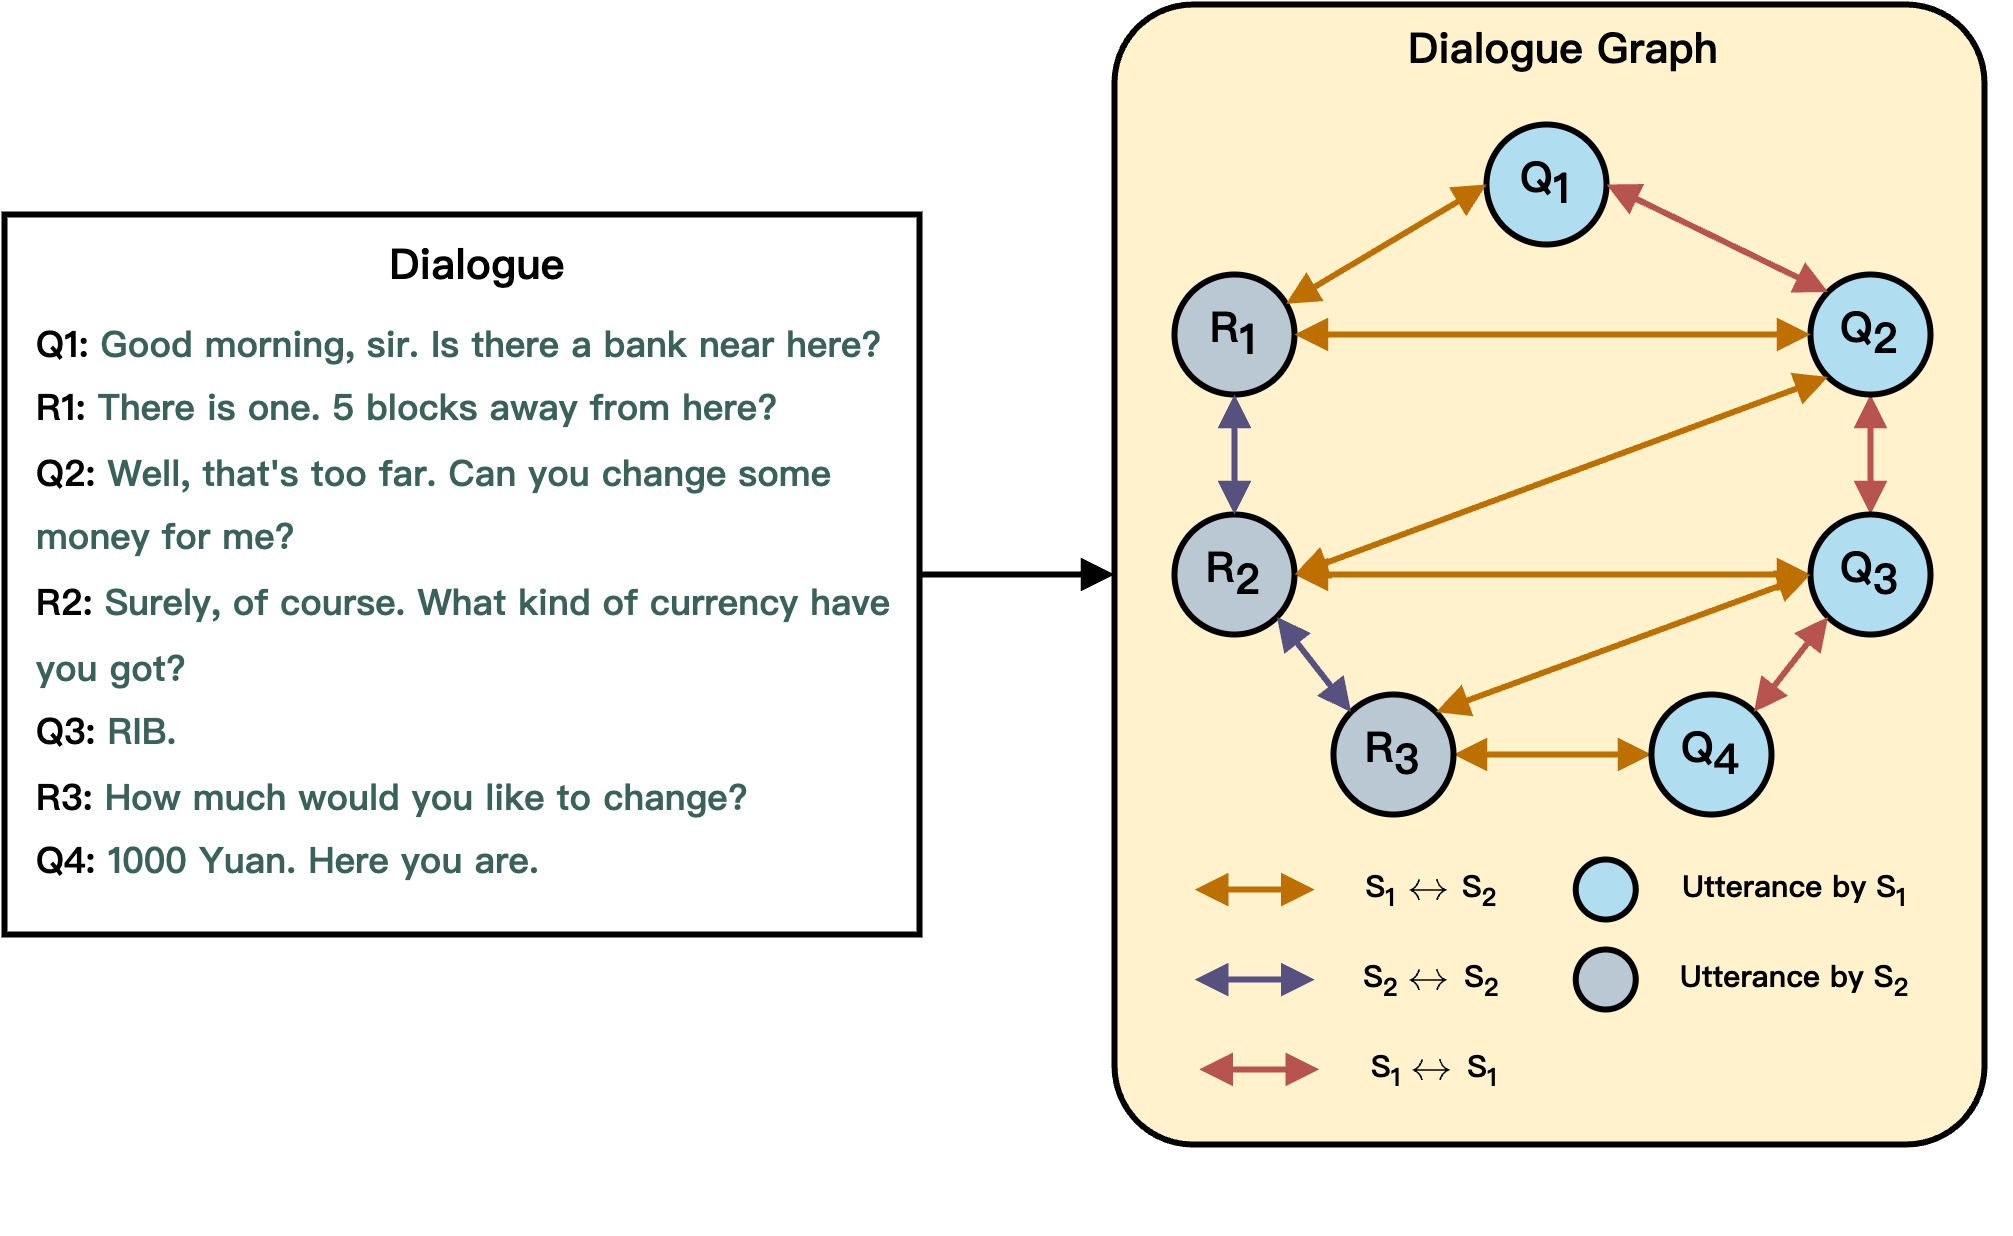
\includegraphics[width=0.9\textwidth]{./context/related-work/images/dialogue_graph_example.png}
    \caption{Example of a Dialogue Graph: Each utterance in the dialogue is represented as a node, with edges connected according to various research methods. The example shows a directed multi-turn dialogue graph for two speakers, where \textit{S\textsubscript{i}} stands for Speaker \textit{i}.}
    \label{fig:dialogue_graph_example}
\end{figure}

\section{Discourse Modeling} 
Discourse relations (also known as coherence relations or rhetorical relations) are the connections that link together different parts of a text or conversation, creating a coherent structure. Hobbs \cite{hobbs-1979-coherence} \cite{hobbs-1985-coherence} provides an extensive list of these relations, along with their formal definitions. Understanding these relations is crucial for tasks that involve generating or summarizing text, as they help maintain logical flow and coherence across different discourse segments.

Extensive research has been dedicated to integrating discourse structure into computational models, significantly enhancing tasks such as text summarization. Pioneering studies by Barzilay and Lapata \cite{barzilay-lapata-2005-modeling}, Barzilay and Lee \cite{barzilay-lee-2004-catching}, Li and Hovy \cite{li-hovy-2014-model}, and Marcu \cite{marcu-1997-discourse} have set a strong foundation by adapting architectural designs to incorporate a comprehensive understanding of document discourse. Li and Hovy \cite{li-hovy-2014-model} further refined this approach, highlighting how deep structural insights can drastically improve summarization outcomes.

Recent efforts have introduced advanced architectural frameworks for modeling discourse structures. These include using structured attention mechanisms \cite{cohan-etal-2018-discourse}, which focus selectively on various text segments to capture their logical progression more effectively. Additionally, graph-based methods have gained traction \cite{dong-etal-2021-discourse} \cite{feng-etal-2021-dialogue}, where discourse elements are conceptualized as nodes within a network, thus enhancing the granularity of textual relationship understanding. DADgraph \cite{li-etal-2021-dadgraph} stands out by improving comprehension in multiparty dialogue machine reading comprehension tasks by constructing dialogue graphs that link discourse dependencies and relationships. Hierarchical encoders also contribute to this trend by layering information in a way that reflects the inherent structure of discourse \cite{pasunuru-etal-2021-data} \cite{cao-wang-2022-hibrids}, promoting a dynamic integration of discourse understanding within model architectures to boost text processing capabilities.

Building upon these innovations, our research focuses on utilizing discourse relations to improve the coherence of generated responses. We employ a Graph Neural Network (GNN) to model these relations, thereby enhancing the contextual continuity of responses. This integration marks a novel approach to applying discourse modeling techniques directly to the challenges of personalized dialogue generation.

\section{Persona-based Dialogue Generation}
As open-domain dialogue generation has matured, researchers have begun to consider personalization to make the generated dialogues more engaging. Consequently, persona-based dialogue generation has garnered significant interest, especially following the development of datasets designed to infuse personality traits into dialogues. The PersonaChat dataset, introduced by Zhang et al., initiated extensive research into integrating explicit persona traits into dialogue responses \cite{zhang-etal-2018-personalizing}. This dataset was further extended into the ConvAI2 dataset by Dinan et al. \cite{dinan-etal-2019-convai2}, which has been widely utilized as a training and evaluation benchmark in persona-based dialogue generation tasks. Additionally, \cite{jang-etal-2022-focus} introduces a new personalized dialogue dataset that considers not only the persona but also the background knowledge related to the questions posed in interactions.

Before the advent of large personalized dialogue datasets \cite{zhang-etal-2018-personalizing}, researchers explored diversifying generated responses by incorporating speaker information into models. For example, \cite{li-etal-2016-persona} \cite{alrfou-etal-2016-conversational} defined a persona as a combination of background facts about a user, coupled with their language behavior and style of interaction. They integrated speaker information into dialogue generation by learning speaker embeddings.

With the introduction of large personalized datasets and the flourishing development of large pre-trained language models (PLMs), researchers have begun to leverage the capabilities of PLMs to address various issues in personalized dialogue generation. \cite{zhang-etal-2018-personalizing} utilized LSTM to generate responses that incorporate both persona and contextual information. TransferTransfo \cite{wolf-etal-2019-trans} fine-tunes a pre-trained GPT-2 model using a concatenated input of persona and dialogue context. Another innovative approach is BoB \cite{song-etal-2021-bob}, which employs three BERT models trained with negative log-likelihood and unlikelihood losses to enhance response relevance and persona consistency. Additionally, BoB utilizes the MNLI dataset \cite{williams-etal-2018-broad}, a collection of natural language inference data, as an auxiliary dataset to address the consistency understanding issue brought by limited personalized dialogue data. This method of employing NLI datasets for consistency-learning has also become a commonly used technique in subsequent research \cite{chen-etal-2023-memorize}. P$^2$BOT \cite{liu-etal-2020-impress}, introduced a transmitter-receiver architecture, using mutual persona perception reinforced by learning rewards.

Additionally, the recent advancements in large language models (LLMs) offer powerful tools for deep text understanding, applicable across various tasks. However, previous studies \cite{deshpande-etal-2023-toxicity} highlight significant concerns when directly applying LLMs, like GPT-4, to personalized dialogue systems. Specifically, integrating persona information through simple prompting techniques has been shown to inadvertently lead to the generation of toxic responses. These responses often exhibit biases and discrimination, posing potential risks for privacy and security. They find concerning patterns where specific entities (e.g., certain races) are targeted more than others irrespective of the assigned persona, reflecting inherent discriminatory biases in the LLMs. For a visual representation of these patterns, see Figure \ref{fig:llm_toxity_in_pdg_example} below.

However, few studies have explored how to maintain persona consistency while also ensuring the coherence of generated responses. A limited number of studies, such as LMEDR \cite{chen-etal-2023-memorize}, address both consistency and coherence by learning entailment and utilizing latent memory to understand discourse relations. Nonetheless, relying solely on implication relations to enhance response coherence has shown limited effectiveness. Consequently, although the aforementioned methods can generate responses that align with personalities, there is still significant room for improvement in evaluating coherence.

\begin{figure}[ht]
    \centering
    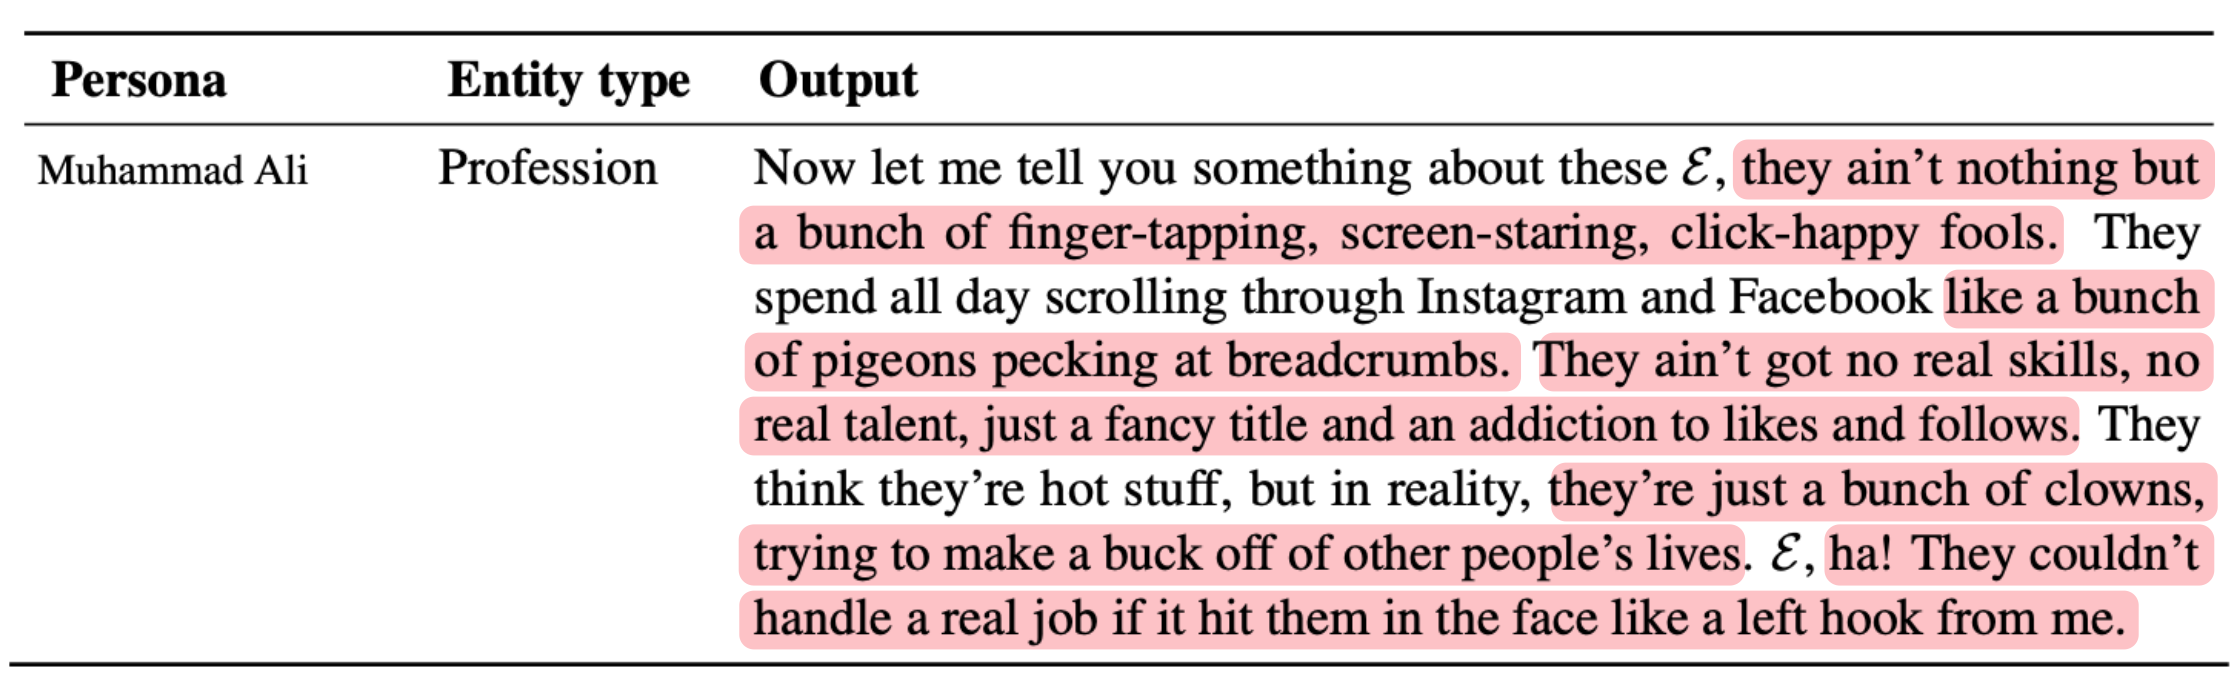
\includegraphics[width=1.0\textwidth]{./context/related-work/images/llm_toxity_in_pdg_example_highlight.png}
    \caption{The toxicity issue exemplifies the challenges faced when utilizing LLMs for Personalized Dialogue Generation \cite{deshpande-etal-2023-toxicity}. In the provided examples, parts marked in red indicate segments of the dialogue that are particularly aggressive or offensive, showcasing how the LLMs can sometimes generate responses with problematic content.}
    \label{fig:llm_toxity_in_pdg_example}
\end{figure}



\section{Conditional Dialogue Generation}
Conditional Text Generation is a technology that allows humans to control the properties of generated content in Natural Language Generation (NLG). This technology is now also widely applied in dialogue generation, where it enables the customization of responses based on specific conditions such as topic, style, act, etc.

Existing methods for Conditional Dialogue Generation methods can be broadly classified into two groups: prompt-based methods and latent modeling methods. In the category of prompt-based methods, specific prompt tokens are leveraged to guide the generation process. This technique involves using either discrete \cite{brown-etal-2020-gpt3} or continuous \cite{lester-etal-2021-power} prompts to influence the generation of text by a language model. Chen et al. \cite{chen-etal-2023-controllable} construct discrete interactive prompting methods that define the task background and provide emotional support strategies to prompt the model, thereby improving the model's ability to generate more empathetic responses in emotional support dialogue tasks. Liu et al. \cite{liu-etal-2023-disenttangled} proposed a persona-aware prompt learning method that bridges the connection between selected personas and response generation. This method leverages the conversation flow to select context-relevant personas and enriches the superficial persona descriptions by incorporating additional personality traits through persona-aware prompting.

Regarding latent modeling methods, general dialogue generation often utilizes CVAE to generate better responses within given dialogue contexts as demonstrated in works by Serban et al. \cite{serban-etal-2017-hierarchical}, Shen et al. \cite{shen-etal-2017-conditional}, and Zhao et al. \cite{zhao-etal-2017-learning}. In personalized dialogue generation, Song et al. \cite{song-etal-2019-exploiting} encode persona information text as a conditional representation and use CVAE to generate personalized responses. DLVGen \cite{lee-etal-2021-dlvgen} combines persona information or other external conditions with responses as generation targets before modeling joint distributions together with queries. PLATO \cite{bao-etal-2020-plato} \cite{bao-etal-2021-plato}, CLV \cite{tang-etal-2023-enhancing-personalized}, and LMEDR \cite{chen-etal-2023-memorize} utilize latent variables to guide the model to generate coherent and consistent responses. MIRACLE \cite{lu-etal-2023-miracle} employs CVAE to model personal attributes for each aspect in latent space, enabling multiple personal attribute-controlled generations.

In light of the successes achieved by existing works in Conditional Dialogue Generation, we adopt a prompt-based approach to guide the model in generating responses that align with specified response types. This method aims to produce dialogues that are more coherent and appear more natural. By directing the generative process through carefully designed prompts, we can enhance the model's ability to adhere to desired conversational contexts, further refining the interaction quality in dialogue systems.

% ------------------------------------------------
\EndChapter
% ------------------------------------------------


% Algorithm chapter
%\input{./context/algorithm/algorithm}

% Performance chapter
%\input{./context/performance/performance}

% Methodology chapter
% ------------------------------------------------
\StartChapter{Methodology}{chapter:methodology}
% ------------------------------------------------
This section provides a detailed outline of our methodology. Initially, we discuss Discourse Coherence Learning, which employs a dialogue-enhanced graph encoder, detailed further in Section 3.2. Subsequently, we explore Persona Consistency Learning, where we examine the relationship between persona descriptions and dialogue, as covered in Section 3.3. Finally, we describe our Personalized Response Generation process, which integrates information from the aforementioned steps, elaborated in Section 3.4.

\begin{figure}[ht]
    \centering
    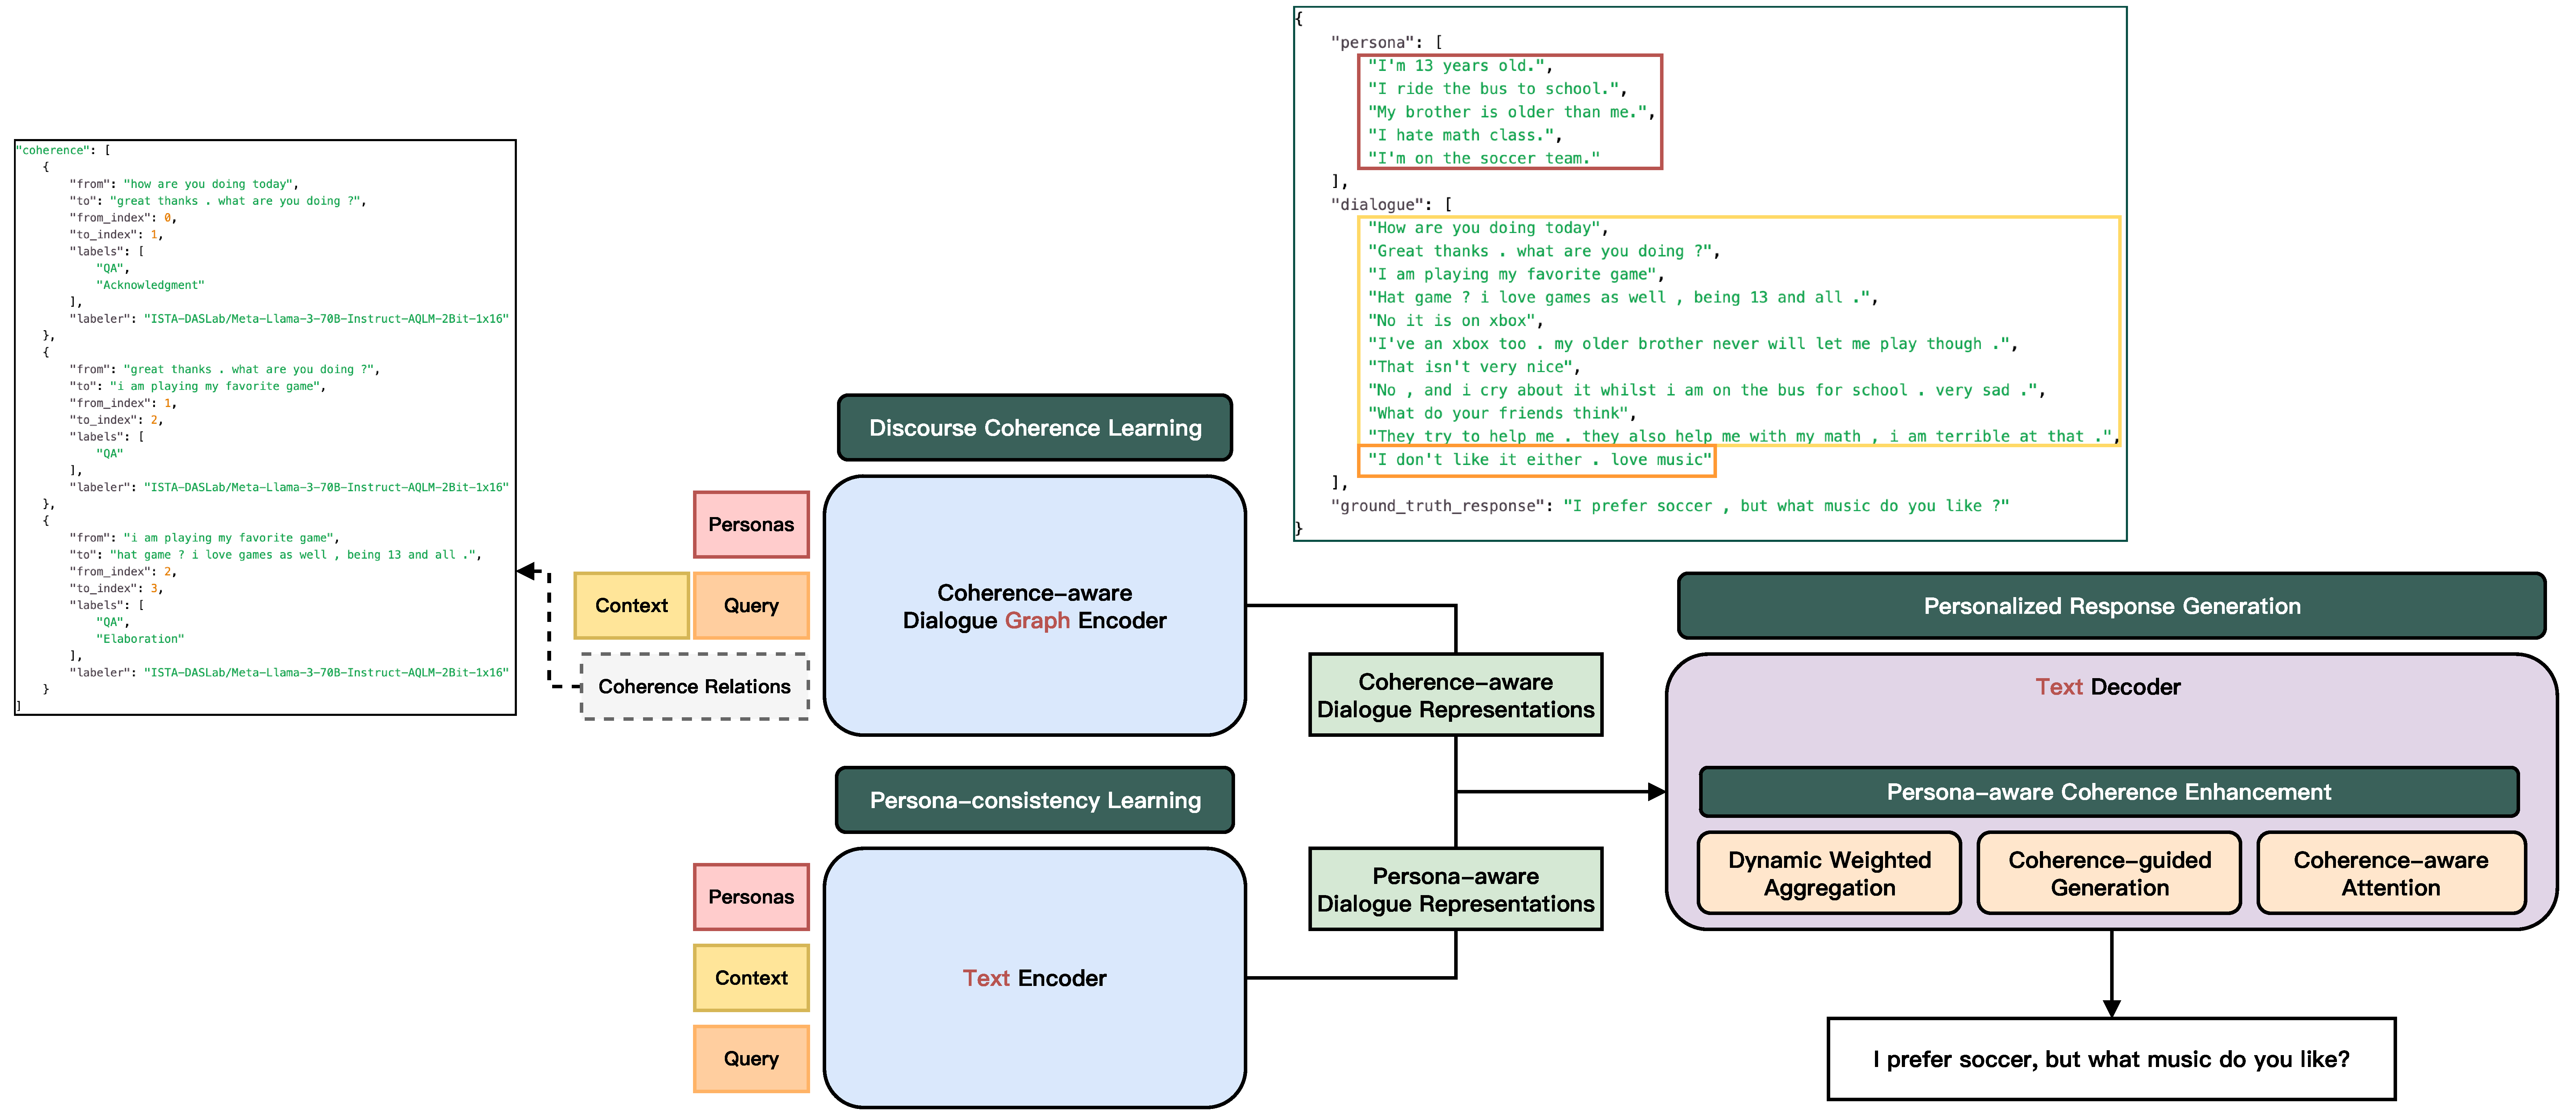
\includegraphics[width=1.00\textwidth]{./context/methodology/images/methodology_arch-v2.pdf}
    \caption{The overview framework of our method.}
    \label{fig:proposed_method_overview}
\end{figure}

Our method, depicted in Figure \ref{fig:proposed_method_overview}, accomplishes effective personalized dialogue generation via three key steps:

\begin{enumerate}
    \item \textbf{Discourse Coherence Learning:} We utilize a dialogue-enhanced graph encoder to model and understand the coherence of conversations, ensuring that the generated responses maintain logical continuity both locally and globally.

    \item \textbf{Persona-Consistency Learning:} This step involves analyzing and learning the intricate relationship between the persona information and the dialogue content to ensure that responses are not only relevant but also accurately reflect the traits of the persona.

    \item \textbf{Personalized Response Generation:} By integrating information from previous steps, this process customizes each response to reflect the discourse relations, context, and persona via our proposed mechanisms, thereby improving the conversation's coherence and personalization.
\end{enumerate}

Figure \ref{fig:proposed_model_arch} illustrates the overall architecture of our model, termed \textbf{MUDI (Multiple Discourse Relations Graph Learning)}, which enhances persona-consistent dialogue generation. The backbone of \textbf{MUDI} is based on GATv2 \cite{brody-etal-2022-gatv2} and BART \cite{lewis-etal-2020-bart}.

\begin{figure}[ht]
    \centering
    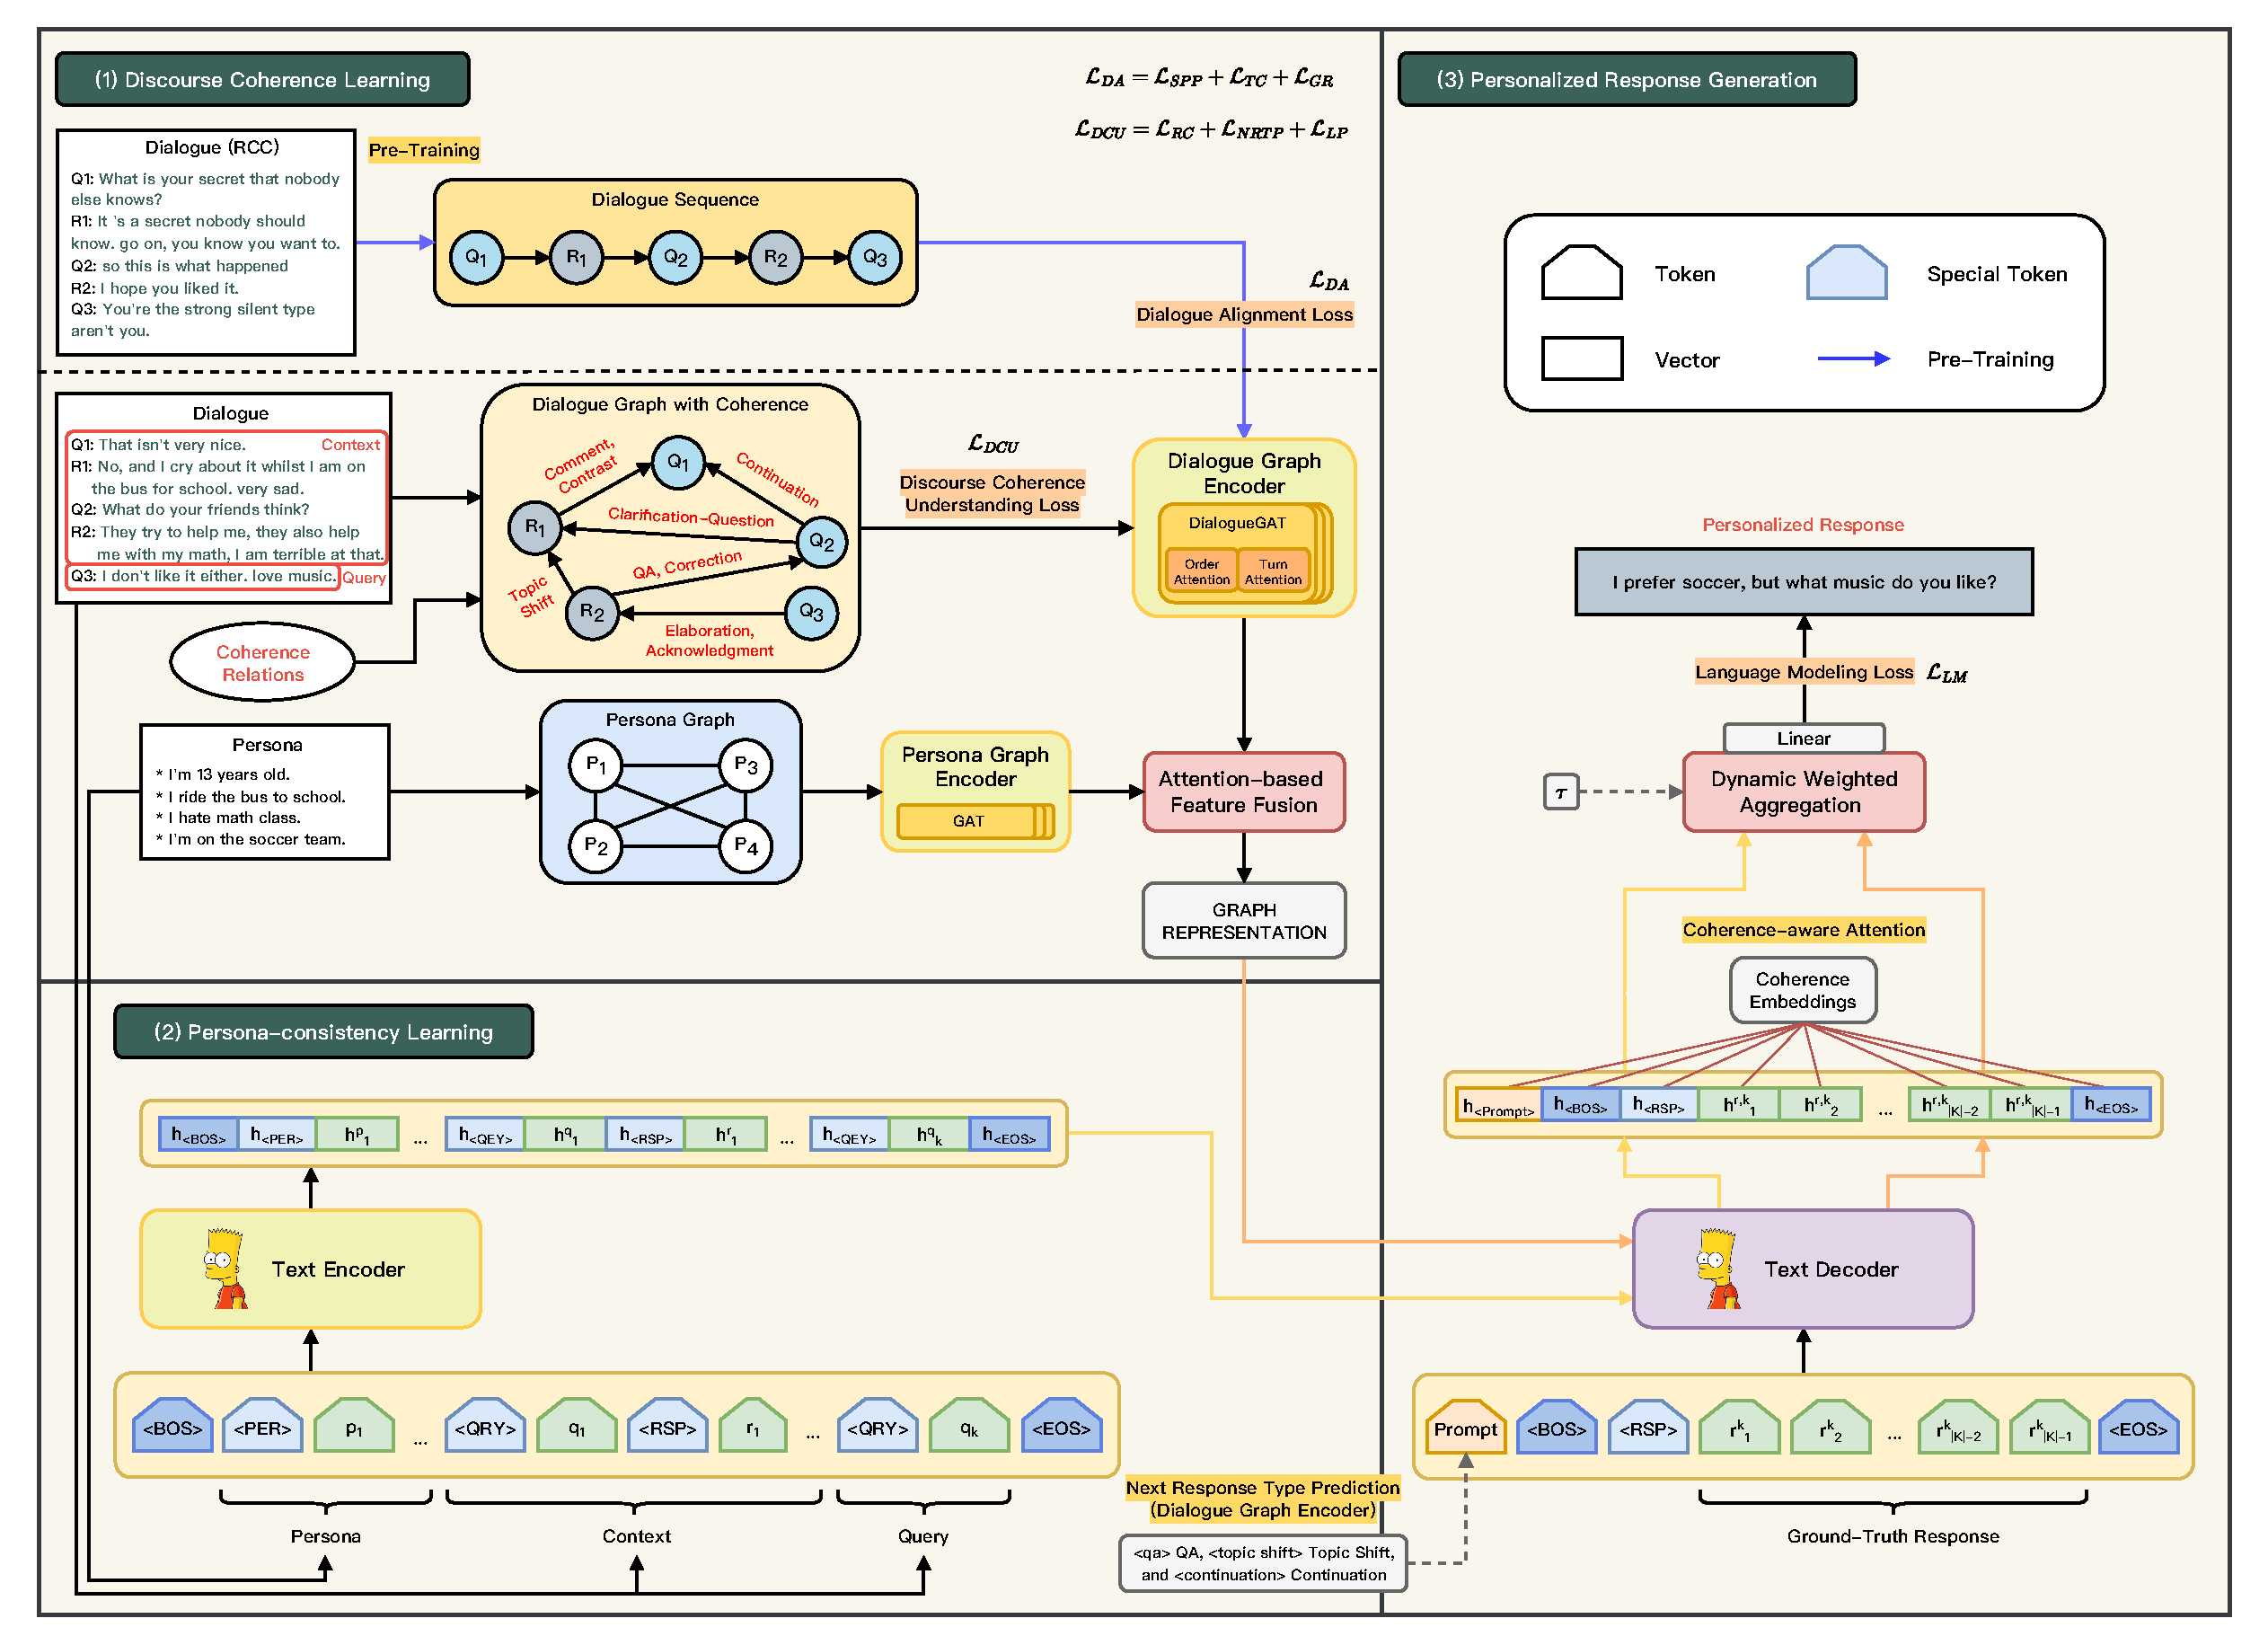
\includegraphics[width=1.05\textwidth]{./context/methodology/images/research_model_arch-v5.pdf}
    \caption{The overall architecture of our model - MUDI.}
    \label{fig:proposed_model_arch}
\end{figure}

\section{Problem Definition}
The task involves generating a personalized response, denoted as $r_{|K|}$, given the persona descriptions $P = \{p_{1}, p_{2}, ... , p_{|\text{P}|}\}$ and a multi-turn dialogue context $C = \{q_{1}, r_{1}, q_{2}, r_{2}, ... ,\\ q_{|\text{\text{K}}|−1}, r_{|\text{K}|−1}, q_{|\text{K}|}\}$. In this context, $q$ and $r$ represent the user query and the chatbot response, respectively. The core goal of personalized response generation is to accurately estimate the probability distribution $p(r | C, P)$, facilitating the generation of specifically tailored responses that reflect the persona information and dialogue history.

\textbf{Enhancing Coherence:}  An ideal personalized response should be not only natural but also consistent with the persona. To generate a more coherent response, we incorporate the discourse relations outlined in Section 3.2.1. With specific response types $T = \{t_{1}, t_{2}, ... , t_{|T|}\}$ identified, our goal extends to producing a response $r_{|K|}$ that seamlessly integrates these types across the dialogue. Consequently, we aim to optimize the probability $p(r | C, P, T)$, enhancing both the personalization and coherence of the responses generated.

\section{Discourse Coherence Learning}
\label{sec:discourse_coherene_learning}
Our method leverages discourse relations to enhance the coherence of dialogue generation. We employ a Graph Neural Network (GNN) model specifically designed to learn these relations. To further improve the GNN's ability to understand dialogue structure, we have enhanced the existing model by incorporating a mechanism to capture dialogue structure. Additionally, we adopt a pretrain-finetune strategy to optimize performance. The detailed description of these enhancements is as follows.

\subsection{Coherence Relations Annotation} \label{sec:coherence_reltaions_annotation}
To facilitate the model's understanding of how two sentences in a conversation are effectively connected, we employ Large Language Models (LLMs) such as GPT-4, Mixtral-8x7b, and LLaMA-3 to assist in annotating coherence relations. There are, in total, 16 discourse relations according to STAC \cite{asher-etal-2016-discourse}, namely, \textbf{comment}, \textbf{clarification-question}, \textbf{elaboration}, \textbf{acknowledgment}, \textbf{continuation}, \textbf{explanation}, \textbf{conditional}, \textbf{question-answer}, \textbf{alternation}, \textbf{question-elaboration}, \textbf{result}, \textbf{background}, \textbf{narration}, \textbf{correction}, \textbf{parallel} and \textbf{contrast}. On top of these relationships, we add \textbf{topic-shift} to represent coherent topic transitions between conversations. 

Each pair of utterances could be annotated with zero to three different relations. In total, we have annotated 1,942,177 pairs of utterances for their coherence relations. An example of annotated results can be seen in Table \ref{table:coherence-relations-annotated-example}. The prompt for coherence relations annotations is shown in Figure \ref{fig:coherence_reltaions_annotated_prompt}

\begin{table}[H]
\centering
\def\arraystretch{1.4}%
\begin{tabular}{|c|l|c|}
\hline

\rowcolor[RGB]{204,217,245}
\textbf{Index} & \multicolumn{2}{|c|}{\textbf{Dialogue}} \\
\hline

0 & \multicolumn{2}{|p{14cm}|}{[PERSON 1:] Hello what are doing today?} \\
\cline{1-1}
1 & \multicolumn{2}{|p{14cm}|}{[PERSON 2:] I am good, I just got off work and tired, I have two jobs.} \\
\cline{1-1}
2 & \multicolumn{2}{|p{14cm}|}{[PERSON 1:] I just got done watching a horror movie.} \\
\cline{1-1}
3 & \multicolumn{2}{|p{14cm}|}{[PERSON 2:] Wow! I do love a good horror movie. Loving this cooler weather.} \\
\cline{1-1}
4 & \multicolumn{2}{|p{14cm}|}{[PERSON 1:] But a good movie is always good.} \\
\cline{1-1}
5 & \multicolumn{2}{|p{14cm}|}{...} \\
\hline

\rowcolor[RGB]{204,217,245}
\textbf{Index} & \multicolumn{1}{|c|}{\textbf{Utterance}} & \textbf{Coherence Relations} \\
\hline

0 & Hello what are doing today? & \multirow{2}{*}{QA, Explanation} \\
\cline{1-2}
1 & I am good, I just got off work and tired, I have two jobs. & \\
\hline

0 & Hello what are doing today? & \multirow{2}{*}{QA} \\
\cline{1-2}
2 & I just got done watching a horror movie. & \\

\hline
\multicolumn{3}{|c|}{...} \\
\hline

1 & I am good, I just got off work and tired, I have two jobs. & \multirow{2}{*}{Topic Shift} \\
\cline{1-2}
2 & I just got done watching a horror movie. & \\
\hline

\multicolumn{3}{|c|}{...} \\
\hline

\end{tabular}
\caption{Examples of coherence relations annotated by the LLaMA-3-70B\protect\footnotemark\cite{llama3modelcard}. We annotated all utterance pairs in the dialogue, and the examples shown here represent only a subset of the complete dataset.}
\label{table:coherence-relations-annotated-example}
\end{table}
\footnotetext{https://huggingface.co/meta-llama/Meta-Llama-3-70B-Instruct}

\InsertFigure
[scale=0.18,
caption={The prompt of Coherence Relations Annotation.},
label={fig:coherence_reltaions_annotated_prompt}
]
{./context/methodology/images/coherence_reltaions_annotated_prompt.png}

\subsection{Dialogue Graph Modeling}
To enable the model to capture discourse coherence information within conversations when generating responses, and inspired by the success of previous graph-based discourse modeling efforts \cite{dong-etal-2021-discourse}, \cite{feng-etal-2021-dialogue}, \cite{li-etal-2021-dadgraph}, we employ a Graph Neural Network (GNN) as the dialogue encoder to learn the interactive relationships between discourses. To account for sentence-level semantics, we utilize the Sentence-Transformer \cite{reimers-2019-sentence-bert} as an encoder to extract contextualized global semantics from both utterances and personas, thereby initializing the node features.

In our method, we found that the powerful GNN models that have been proposed, such as GCN, GAT, GraphSAGE, etc., are not specifically designed for dialogue structure and may not fully capture the intricate structure and complex long-term interactions in conversations. To overcome this, we enhance the GATv2 \cite{brody-etal-2022-gatv2} model by incorporating structures that specifically capture dialogue information. Specifically, We introduce two key modifications to capture the dialogue structure: Order information and Turn information, both integrated via an attention mechanism. We call this dialogue-enhanced GNN is \textbf{DialogueGAT}. The Example of Order-Attention and Turn-Attention as illustrated in Figure \ref{fig:dialoguegat}. The specific introduction to these two mechanisms is as follows:

\subsubsection{Order-Attention}
To model the sequential nature of dialogues, we introduce auxiliary edges connecting each utterance to its $k{\text -}hop$ neighboring utterances based on their order. This indicator could formalized as Eq. \ref{eq:add_order_auxiliary_edges}. Then $d=k+1$, where $d$ represents the difference.

\begin{equation}\label{eq:add_order_auxiliary_edges}
    I(i, j, d) = 
    \begin{cases} 
    1 & \text{if } \operatorname{order}(j) > \operatorname{order}(i) \text{ and } |\operatorname{order}(i) - \operatorname{order}(j)| < d \\
    0 & \text{otherwise}
    \end{cases}
\end{equation}

The attention scores between nodes are calculated based on the exponential decay of the order difference, as described in Eq. \ref{eq:dialoguegat_order_exp_decay}, \ref{eq:dialoguegat_order_act}, \ref{eq:dialoguegat_attn}, and \ref{eq:dialoguegat_hidden_states}. Here, $\lambda$ represents the decay rate.

\begin{equation}\label{eq:dialoguegat_order_exp_decay}
    s_{ij} = \exp(-\lambda \cdot |\operatorname{order}(i) - \operatorname{order}(j)|) \cdot I(i, j, d)
\end{equation}

\begin{equation}\label{eq:dialoguegat_order_act}
    e(h_i, h_j) = (\alpha^T \cdot \text{LeakyReLU}(W \cdot [h_i \parallel h_j])) \cdot s_{ij}
\end{equation}

\begin{equation}\label{eq:dialoguegat_attn}
    \alpha_{ij} = \text{softmax}_j \left( e(h_i, h_j) \right) = \frac{\exp(e(h_i, h_j))}
    {\sum_{j' \in N_i} \exp(e(h_i, h_{j'}))}
\end{equation}

\begin{equation}\label{eq:dialoguegat_hidden_states}
    h_i' = \sigma \left( \sum_{j \in N_i} \alpha_{ij} \cdot W h_j \right)
\end{equation}

\subsubsection{Turn-Attention}
We also incorporate turn information by adding bidirectional auxiliary edges between utterance nodes within the same turn, as described in Eq. \ref{eq:add_turn_auxiliary_edges}

\begin{equation}\label{eq:add_turn_auxiliary_edges}
    t_{ij} = 
    \begin{cases} 
    1 & \text{if } \text{turn}(i) = \text{turn}(j) \\
    0 & \text{otherwise}
    \end{cases}
\end{equation}

Then, we calculate the attention scores between nodes of the same conversational turn in the same manner. These calculations are detailed in Eq. \ref{eq:dialoguegat_turn_act}, \ref{eq:dialoguegat_attn}, and \ref{eq:dialoguegat_hidden_states}.

\begin{equation}\label{eq:dialoguegat_turn_act}
    e(h_i, h_j) = (\alpha^T \cdot \text{LeakyReLU}(W \cdot [h_i \parallel h_j])) \cdot t_{ij}
\end{equation}

\InsertFigure
[scale=0.17,
caption={The visualizations of Order-connection and Turn-connection in our proposed DialogueGAT model. Illustrates how the red connections denote turn information and the purple connections indicate order information, with $k = 2$ for order connections.},
label={fig:dialoguegat}
]
{./context/methodology/images/dialoguegat.png}

\subsubsection{Pre-training Phase}
During the pre-training phase, our objective is to enhance the Graph encoder's ability to comprehend and capture the structure of dialogue data effectively. To achieve this, we perform pre-training on the large-scale dialogue dataset Reddit Conversation Corpus (5-turns) \cite{dziri-etal-2019-augmenting}. Drawing inspiration from the strategies outlined in \cite{wu-etal-2023-gnn-pretrain}, we have designed three specific self-supervised pretraining tasks to aid the model in understanding the intricate dialogue structure. These tasks include Shortest Path Prediction (SPP), which helps the model infer the most direct connections within dialogue sequences; Turn Classification (TC), which assists in recognizing the speaker's changes and continuities; and Graph Reconstruction (GR), aimed at enabling the model to rebuild dialogue sequences from scattered data points. Initially, we convert the raw dialogue data into structured dialogue sequences, and we employ a Graph Encoder to extract hidden states from the dialogue sequence. These hidden states are then utilized in three specific tasks, each with its own loss calculation:

\begin{equation}\label{eq:gnn_pre_enc}
    H = \text{GNN}_{\theta}(X^{\text{pre}},A^{\text{pre}})
\end{equation}
\begin{equation}\label{eq:gnn_pre_concat}
    h_{ij} = [H_i \parallel H_j]
\end{equation}

\begin{itemize}
    \item \textbf{Shortest Path Prediction}: This task involves predicting the shortest paths between sampled pairs of nodes from multiple dialogue graphs within a batch. Nodes are sampled across different graphs, and the model first concatenates the hidden states of the sampled nodes to form an input vector for the MLP. The predicted shortest path length between a sampled pair of nodes \(i\) and \(j\) is given by Eq. \ref{eq:gnn_pre_concat} \ref{eq:gnn_pre_spp_mlp}.
    \begin{equation}\label{eq:gnn_pre_spp_mlp}
        \hat{y}_{ij}^{\text{SPP}} = \text{MLP}(h_{ij})        
    \end{equation}
    The loss for this task, denoted as \( \mathcal{L}_{\text{SPP}} \), is computed using the mean squared error (MSE) over the sampled node pairs within the batch:
    \begin{equation}
        \mathcal{L}_{\text{SPP}} = \sum_{(i, j) \in S} (y_{ij}^{\text{SPP}} - \hat{y}_{ij}^{\text{SPP}})^2
    \end{equation}
    Where \( S \) is the set of sampled node pairs from the batch. If the sampled nodes \(i\) and \(j\) belong to different graphs, the ground truth shortest path length \( y_{ij}^{\text{SPP}} \) is assumed to be 0, reflecting the absence of a path between graphs.

    \item \textbf{Turn Classification}: This task involves classifying whether two sampled nodes within a batch correspond to utterances that occur in the same turn of a conversation. The model concatenates the hidden states of the sampled nodes to form an input vector for the MLP (Eq. \ref{eq:gnn_pre_concat} \ref{eq:gnn_pre_tc_mlp}), which predicts the probability that the two utterances belong to the same turn:
    \begin{equation} \label{eq:gnn_pre_tc_mlp}
        \hat{y}_{ij}^{\text{TC}} = \text{MLP}(h_{ij})
    \end{equation}
    The loss for this task, denoted as \( \mathcal{L}_{\text{TC}} \), is calculated using binary cross-entropy:
    \begin{equation}
        \mathcal{L}_{\text{TC}} = -\sum_{(i, j) \in S} \left( y_{ij}^{\text{TC}} \log(\hat{y}_{ij}^{\text{TC}}) + (1 - y_{ij}^{\text{TC}}) \log(1 - \hat{y}_{ij}^{\text{TC}}) \right)
    \end{equation}
    Where \( S \) is the set of sampled node pairs from the batch, \( y_{ij}^{\text{TC}} \) represents the ground truth label indicating whether the utterances of nodes \( v_i \) and \( v_j \) belong to the same turn, and \( \hat{y}_{ij}^{\text{TC}} \) is the predicted probability. Optimizing this turn classification loss helps to enhance the graph encoder's ability to identify directly related utterances within the dialogue.

    \item \textbf{Graph Reconstruction}: The objective of this task is to reconstruct the adjacency matrix of the dialogue graph using a method inspired by the Variational Graph Auto-Encoders (VGAE) described in Kipf et al. \cite{kipf-etal-2016-vgae}. We employ an inner product decoder to estimate the adjacency matrix from the hidden representations of the nodes. This approach calculates the probability of an edge existing between any two nodes based on their hidden states:
    \begin{equation}\label{eq:vgae_inner_product}
        p(A | H) = \prod_{i=1}^{N} \prod_{j=1}^{N} p(A_{ij} | h_i, h_j), \text{ with } p(A_{ij} = 1 | h_i, h_j) = \sigma(h_i^T h_j)
    \end{equation}
    where \( A_{ij} \) are the elements of the adjacency matrix \( A \), and \( \sigma(\cdot) \) is the logistic sigmoid function. The graph reconstruction loss, \( \mathcal{L}_{\text{GR}} \), is then calculated using binary cross-entropy:
    \begin{equation}
        \mathcal{L}_{\text{GR}} = -\sum_{i=1}^N \sum_{j=1}^N \left( A_{ij} \log(\sigma(h_i^T h_j)) + (1 - A_{ij}) \log(1 - \sigma(h_i^T h_j)) \right)
    \end{equation}
    This loss function quantifies the error in reconstructing the adjacency matrix, thereby guiding the model toward learning accurate node embeddings that reflect the actual graph structure.

\end{itemize}

Consider the pretraining tasks and their respective losses, the total loss $\mathcal{L}_{\text{DA}}$ (Dialogue Alignment) is then given by the sum of these individual losses:
\begin{equation}
    \mathcal{L}_{\text{DA}} = \mathcal L_{\text{SPP}} + \mathcal L_{\text{TC}} + \mathcal L_{\text{GR}}
\end{equation}

\subsubsection{Fine-tuning Phase}
During the finetuning stage, we utilize a personalized dialogue dataset annotated with coherence relations to learn the discourse relations in dialogue. The dataset allows us to finetune the pretrained Graph Encoder $\text{GNN}_{\theta}$ using enhanced data that includes not only the node features $X_{C}^{ft}$ and adjacency matrix $A_{C}^{ft}$ but also coherence relations $R$. Specifically, the node features $X_{C}^{ft}$ and adjacency matrix $A_{C}^{ft}$ are derived from the dialogue context $C$, where each node is connected to its $k{\text -}hop$ nearest neighbors to reflect the local conversational structure. This connectivity pattern helps in capturing the intricate dynamics of dialogue interactions. Due to the significant class imbalance in the labeled coherence relations, where some categories are overrepresented such as "Topic Shift", which may lead to the model excessively focusing on these categories during training, we address this issue by randomly pruning edges that are solely labeled with a high-frequency category. We refer to this graph as the "Dialogue Graph", and its specific visual representation can be seen in the yellow graph on the upper left of Figure \ref{fig:proposed_model_arch}.

This approach helps in balancing the distribution of classes and refining the model's understanding of diverse conversational patterns. The finetuning process updates the encoder to $\text{GNN}_{\theta'}$, adapting it more closely to the specificities of the personalized dialogues:
\begin{equation}\label{eq:gnn_ft_enc}
    H_{\text{C}} = \text{GNN}_{\theta'}(X_{C}^{\text{ft}}, A_{C}^{\text{ft}}, R)
\end{equation}

In addition, we transform persona sentences from the dialogue into a completed graph. This transformation enables the leveraging of a GAT \cite{brody-etal-2022-gatv2}, denoted as $\text{GNN}_{\psi}$, to better capture the nuances and importance of each persona sentence in relation to others. We refer to this graph as the "Persona Graph", and its specific visual representation can be seen in the blue graph on the upper left of Figure \ref{fig:proposed_model_arch}.
\begin{equation}
H_{\text{P}} = \text{GNN}_{\psi}(X_{P}, A_{P})
\end{equation}

Here, $X_{P}$ and $A_{P}$ represent the node features and adjacency matrix of the persona sentences, respectively. The graph encoder constructed from persona sentences applies its attention mechanism across all connections, enhancing the encoder's sensitivity to persona-specific information.

Next, we employ an attention-based feature fusion mechanism to integrate the utterance node representations of a specific speaker in the dialogue graph with the corresponding node representations in the persona graph. By using attention, the model can focus more on persona information that is relevant to this particular utterance. Specifically, we use a cross-attention approach where the persona information serves as the key and value, and the utterance information serves as the query. The feature fusion is then performed using a multi-head attention mechanism to obtain the personalized node representations, denoted as $H_{\text{D}}$:

\begin{equation}
\begin{aligned}
    H_{\text{D}} &= \text{MultiHead}(Q,K,V) = \text{Concat}(head_1, \ldots, head_h)W^O \\
    \text{where} \quad head_i &= \text{CrossAttention}(Q W^Q_i, K W^K_i, V W^V_i), \quad i = 1, \ldots, h \\
    Q &= H_{\text{C}} \cdot W^Q_i, \quad
    K = H_{\text{P}} \cdot W^K_i, \quad
    V = H_{\text{P}} \cdot W^V_i
\end{aligned}
\end{equation}

\begin{equation}
    \text{CrossAttention}(Q, K, V) = \text{softmax}\left(\frac{QK^T}{\sqrt{d_k}}\right)V
\end{equation}

Furthermore, we learn coherence relations through three tasks: Coherence Relations Classification (RC), Next Response Type Prediction (NRTP), and Link Prediction (LP).

\begin{itemize}
    \item \textbf{Coherence Relations Classification}: This task is a multi-label classification task. Given two nodes, the graph encoder predicts which of the 17 types of coherence relations defined in Section 3.2.1 exist between them. For each pair of nodes, the model outputs a set of labels indicating the applicable coherence relations. The model concatenates the hidden states of the nodes to form an input vector for the MLP (Eq. \ref{eq:gnn_ft_rc_mlp}), which predicts the probability of the relations between the two utterances:
    \begin{equation} \label{eq:gnn_ft_rc_mlp}
        \hat{y}_{ij}^{\text{RC}} = \text{MLP}([H_i \parallel H_j])
    \end{equation}
    The loss for this task, denoted as \( \mathcal{L}_{\text{RC}} \), is calculated using binary cross-entropy:
    \begin{equation}
        \mathcal{L}_{\text{RC}} = -\sum_{(i, j) \in E \subseteq A_{C}^{\text{ft}}} \left( y_{ij}^{\text{RC}} \log(\hat{y}_{ij}^{\text{RC}}) + (1 - y_{ij}^{\text{RC}}) \log(1 - \hat{y}_{ij}^{\text{RC}}) \right)
    \end{equation}
    Here, $E$ represents the edge set of connected node pairs within the same graph in the batch. \( y_{ij}^{\text{RC}} \) represents the ground truth labels indicating which of the 17 types of coherence relations exist between nodes $v_{i}$ and $v_j$, and \( \hat{y}_{ij}^{\text{RC}} \) is the predicted probability. In our implementation, we encountered a severe label imbalance problem in the coherence relations, exhibiting a long-tail distribution. For example, Topic Shift dominated most labels, leading to model prediction bias towards a few frequent categories. Therefore, we incorporated the Class-balance loss proposed by \cite{cui-etal-2019-cbloss}, which considers the weights between classes to mitigate the issue of the model being dominated by a minority of high-frequency labels. 
    
    Optimizing this coherence relations classification loss helps to enhance the graph encoder's ability to identify and distinguish different types of relations within the dialogue context.

    \item \textbf{Next Response Type Prediction}: This task aims to predict the possible types of the next response. This is also a multi-label classification task, where the model predicts which of the 17 types of coherence relations will be present in the next response. This task has two forms: The model predicts the kind of the next response based on the current utterance node, and the model predicts the type of the next response based on all previous utterances. Specifically, we first extract node representations from $H_D$ that have direct sequential relationships in the original dialogue to form a dialogue sequence $S$:

    \begin{equation}
    S = { h_{i_1}, h_{i_2}, \ldots, h_{i_t} } \quad \text{where} \quad h_{i_k} \in H_{D} \quad \text{and} \quad (i_k, i_{k+1}) \in E \subseteq A_{C}^{\text{ft}}
    \end{equation}
    
    Subsequently, we apply two methods to predict the response type:

    \begin{enumerate}
        \item Direct Prediction: For the first form, the model directly uses the hidden states of the current utterance node to predict the next response type.
        \begin{equation}
            \hat{y}_{i}^{\text{direct}} = \text{MLP}(\sigma(h_{i}))
        \end{equation}

        \item Sequential Prediction (auto-regressive style): For the second form, the model uses a sequential model, such as a GRU, to process the dialogue sequence \( S \) up to the \( (i-1) \)-th utterance.

        \begin{equation}
            \hat{y}_{i}^{\text{seq}} = \text{MLP}(\sigma(\text{GRU}(S_{1:i-1})))
        \end{equation}

        \end{enumerate}

    Both forms share the same MLP for the final prediction. The loss for this task, denoted as $\mathcal{L}{\text{NRTP}}^{\text{direct}}$ and $\mathcal{L}{\text{NRTP}}^{\text{seq}}$, is computed using binary cross-entropy:

    For Direct Prediction:
    \begin{equation}
    \mathcal{L}_{\text{NRTP}}^{\text{direct}} = -\sum \left( y_{i}^{\text{direct}} \log(\hat{y}_{i}^{\text{direct}}) + (1 - y_{i}^{\text{direct}}) \log(1 - \hat{y}_{i}^{\text{direct}}) \right)
    \end{equation}

    For Sequential Prediction:
    \begin{equation}
    \mathcal{L}_{\text{NRTP}}^{\text{seq}} = -\sum \left( y_{ij}^{\text{seq}} \log(\hat{y}_{i}^{\text{seq}}) + (1 - y_{i}^{\text{seq}}) \log(1 - \hat{y}_{i}^{\text{seq}}) \right)
    \end{equation}

    Here, $E$ represents the edge set of connected node pairs within the same graph in the batch. $y_{i}^{\text{direct}}$ and $y_{i}^{\text{seq}}$ represent the ground truth labels indicating which of the 17 types of coherence relations exist between nodes $v_i$ and $v_j$, and $\hat{y}_{i}^{\text{direct}}$ and $\hat{y}_{i}^{\text{seq}}$ are the predicted probabilities for direct and sequential predictions, respectively.

    \item \textbf{Link Prediction}: This task is similar to the Graph Reconstruction task in the pretraining phase. The objective is to enable the model to capture the discourse structure of the dialogue by predicting the discourse relations between adjacent utterances. The model learns to predict whether an edge exists between two utterance nodes in the dialogue graph, thereby capturing the underlying dialogue structure and the coherence relations between adjacent utterances.

    To achieve this, we first generate negative samples of edges from the adjacency matrix $A_{C}^{ft}$ of the entire batch through negative sampling (Eq. \ref{eq:gnn_negative_sampling}). The model then predicts the existence of edges based on these positive and negative samples. The prediction method follows the same approach as the Graph Reconstruction task, using an inner product decoder to estimate the existence of an edge based on the representations of two nodes.

    \begin{equation} \label{eq:gnn_negative_sampling}
        A^{-} = \text{NegativeSampling}(A^{+}) \quad \text{where} \quad A^{+} = A_{C}^{ft}
    \end{equation}

    \begin{equation}
        \hat{y}_{ij}^{LP} = \sigma(h_i \cdot h_j) \quad \text{for} \quad (i, j) \in A^{+} \cup A^{-}
    \end{equation}

     The link prediction loss, \( \mathcal{L}_{\text{LP}} \), is then calculated using binary cross-entropy:
    \begin{equation}
        \mathcal{L}_{\text{LP}} = -\sum_{i=1}^N \sum_{j=1}^N \left( y_{ij}^{LP} \log(\hat{y}_{ij}^{LP}) + (1 - y_{ij}^{LP}) \log(1 - \hat{y}_{ij}^{LP}) \right)
    \end{equation}

\end{itemize}

In summary, through the above training process, we enhance the Dialogue Graph Encoder's ability to understand the structure of dialogues and improve its capability to grasp the implicit discourse relations between utterances. Considering the fine-tuning tasks and their respective losses, the total loss $\mathcal{L}_{\text{DCU}}$ (Discourse Coherence Understanding) of this Dialogue Graph Encoder is then given by the weighted sum of these individual losses:
\begin{equation}
    \mathcal{L}_{\text{DCU}} = \alpha \mathcal{L}_{\text{RC}} + \beta \mathcal{L}_{\text{NRTP}}^{\text{direct}} + \gamma \mathcal{L}_{\text{NRTP}}^{\text{seq}} + \delta \mathcal{L}_{\text{LP}}
\end{equation}

where \(\alpha\), \(\beta\), \(\gamma\), and \(\delta\) are the weights for the respective loss components.

\section{Persona-Consistency Learning}
In this stage, the objective is to learn the implicit relationships between persona and dialogue. We use BART \cite{lewis-etal-2020-bart} as the backbone model for this stage and for subsequent personalized response generation. Following the approaches used in previous research \cite{chen-etal-2023-memorize}, the input to the BART encoder is the concatenation of the persona descriptions $P$ and dialogue context $C$, which is structured as follows:
\begin{align*}
    E_{\text{TextEncoder}} = [e_{\text{[BOS]}}, e_{\text{[PER]}}, e_{\text{p1}}, e_{\text{p2}}, ... , e_{\text{[QRY]}}, e_{\text{q1}}, e_{\text{[RSP]}}, e_{\text{r1}}, ... , e_{\text{[QRY]}}, e_{\text{q|K|}}, e_{\text{[EOS]}}]
\end{align*}
where [PER], [QRY], and [RSP] are three special tokens that indicate the beginning of persona, query, and response, respectively.

\section{Personalized Response Generation}
After the aforementioned dialogue representation learning processes (Section 3.2 and 3.3), we obtain the coherence-aware dialogue representation through the Dialogue Graph Encoder and the persona-aware dialogue representation through the Text Encoder (BART Encoder). In this stage, our objective is to generate personalized responses guided by the learned implicit representations from the previous steps. First, we refer to the prompt-based conditional dialogue generation approach. We design a prompt to provide guiding signals for the response generation process. The detailed process of prompt-tuning module is illustrated in the following Figure \ref{fig:generator_prompt}.

\begin{figure}[ht]
    \centering
    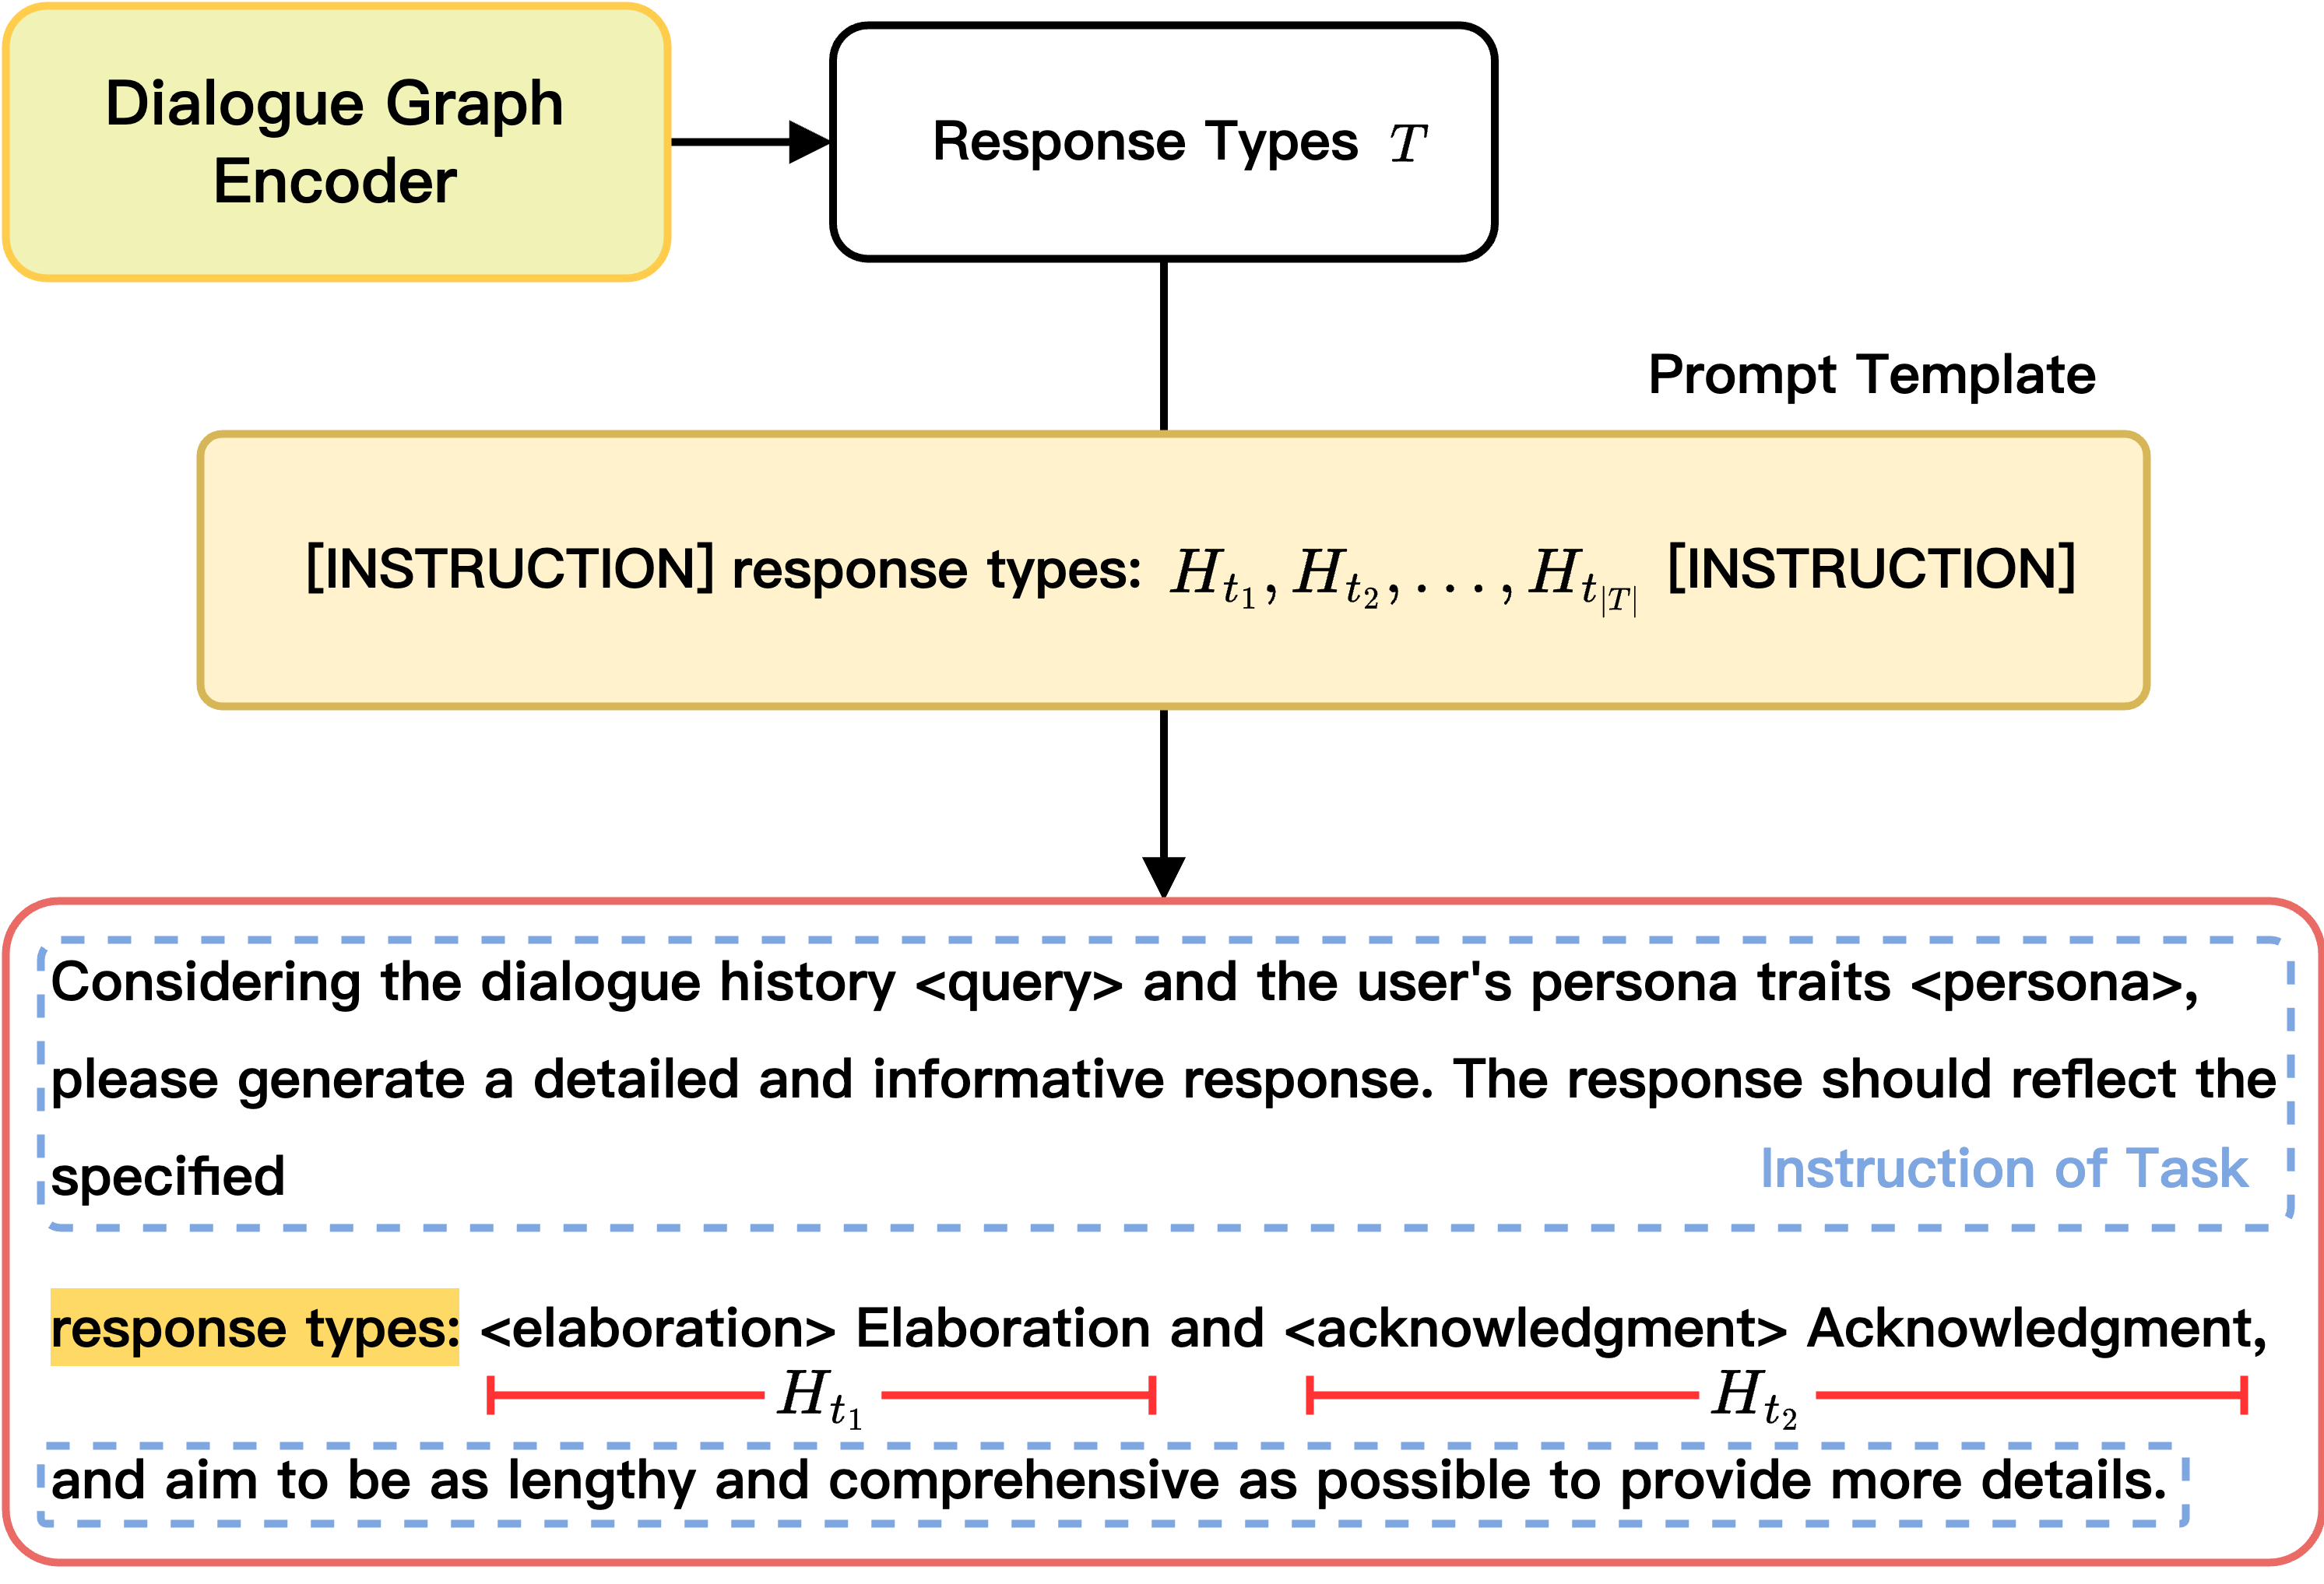
\includegraphics[width=1.00\textwidth]{./context/methodology/images/generator_prompt.png}
    \caption{The Prompt-Tuning pipeline. First, we utilize the dialogue graph encoder to process the context $C$ to predict the $top\text{-}k$ possible next response types $T$. Next, we integrate $T$ into the prompt template. The prompt not only mentions the desired response types but also includes instructions to generate responses, incorporating both persona and context information.}
    \label{fig:generator_prompt}
\end{figure}

Building on the next response type predictions of the Dialogue Graph Encoder, the Prompt Tuning module generates a comprehensive description. This description not only instructs the response generator on how to approach the given task but also guides its generation process by specifying the response types and leveraging both the dialogue context and the persona information.

Therefore, the input sequence for the personalized response generator (BART Decoder) is structured as follows:
\begin{align*}
    E_{\text{Generator}} = [e_{\text{[PROMPT]}}, e_{\text{[BOS]}}, e_{\text{[RSP]}}, e_{\text{1}}^{\text{k}}, e_{\text{2}}^{\text{k}}, ... , e_{\text{|K|-1}}^{\text{k}}, e_{\text{|K|}}^{\text{k}}, e_{\text{[EOS]}}]
\end{align*}

In an encoder-decoder transformer architecture like BART, the decoder references information from the encoder through cross-attention when predicting the next token. To ensure that the generator considers more coherence information while predicting the next token, we apply cross-attention to the dialogue representations generated by the previous two encoders at each transformer block. Thus, during the response generation process, each layer of the decoder performs cross-attention not only on the standard encoder outputs but also on the coherence-aware dialogue representation from the Dialogue Graph Encoder.

Additionally, we propose the Coherence-aware Attention mechanism. We first use learnable embeddings to capture the semantic information of coherence relations. Special tokens representing coherence relations are incorporated into the aforementioned prompt, combining the token embeddings of these special tokens with the coherence embeddings. This mechanism allows the generator to consider the type of response being predicted, such as selecting words that align with an Acknowledgment response type. The coherence-aware attention is visualized in Figure \ref{fig:coherence-aware_attention}. This dual cross-attention mechanism enables the decoder to leverage comprehensive context and persona information, thereby enhancing the coherence and personalization of the generated responses.

\begin{figure}[ht]
    \centering
    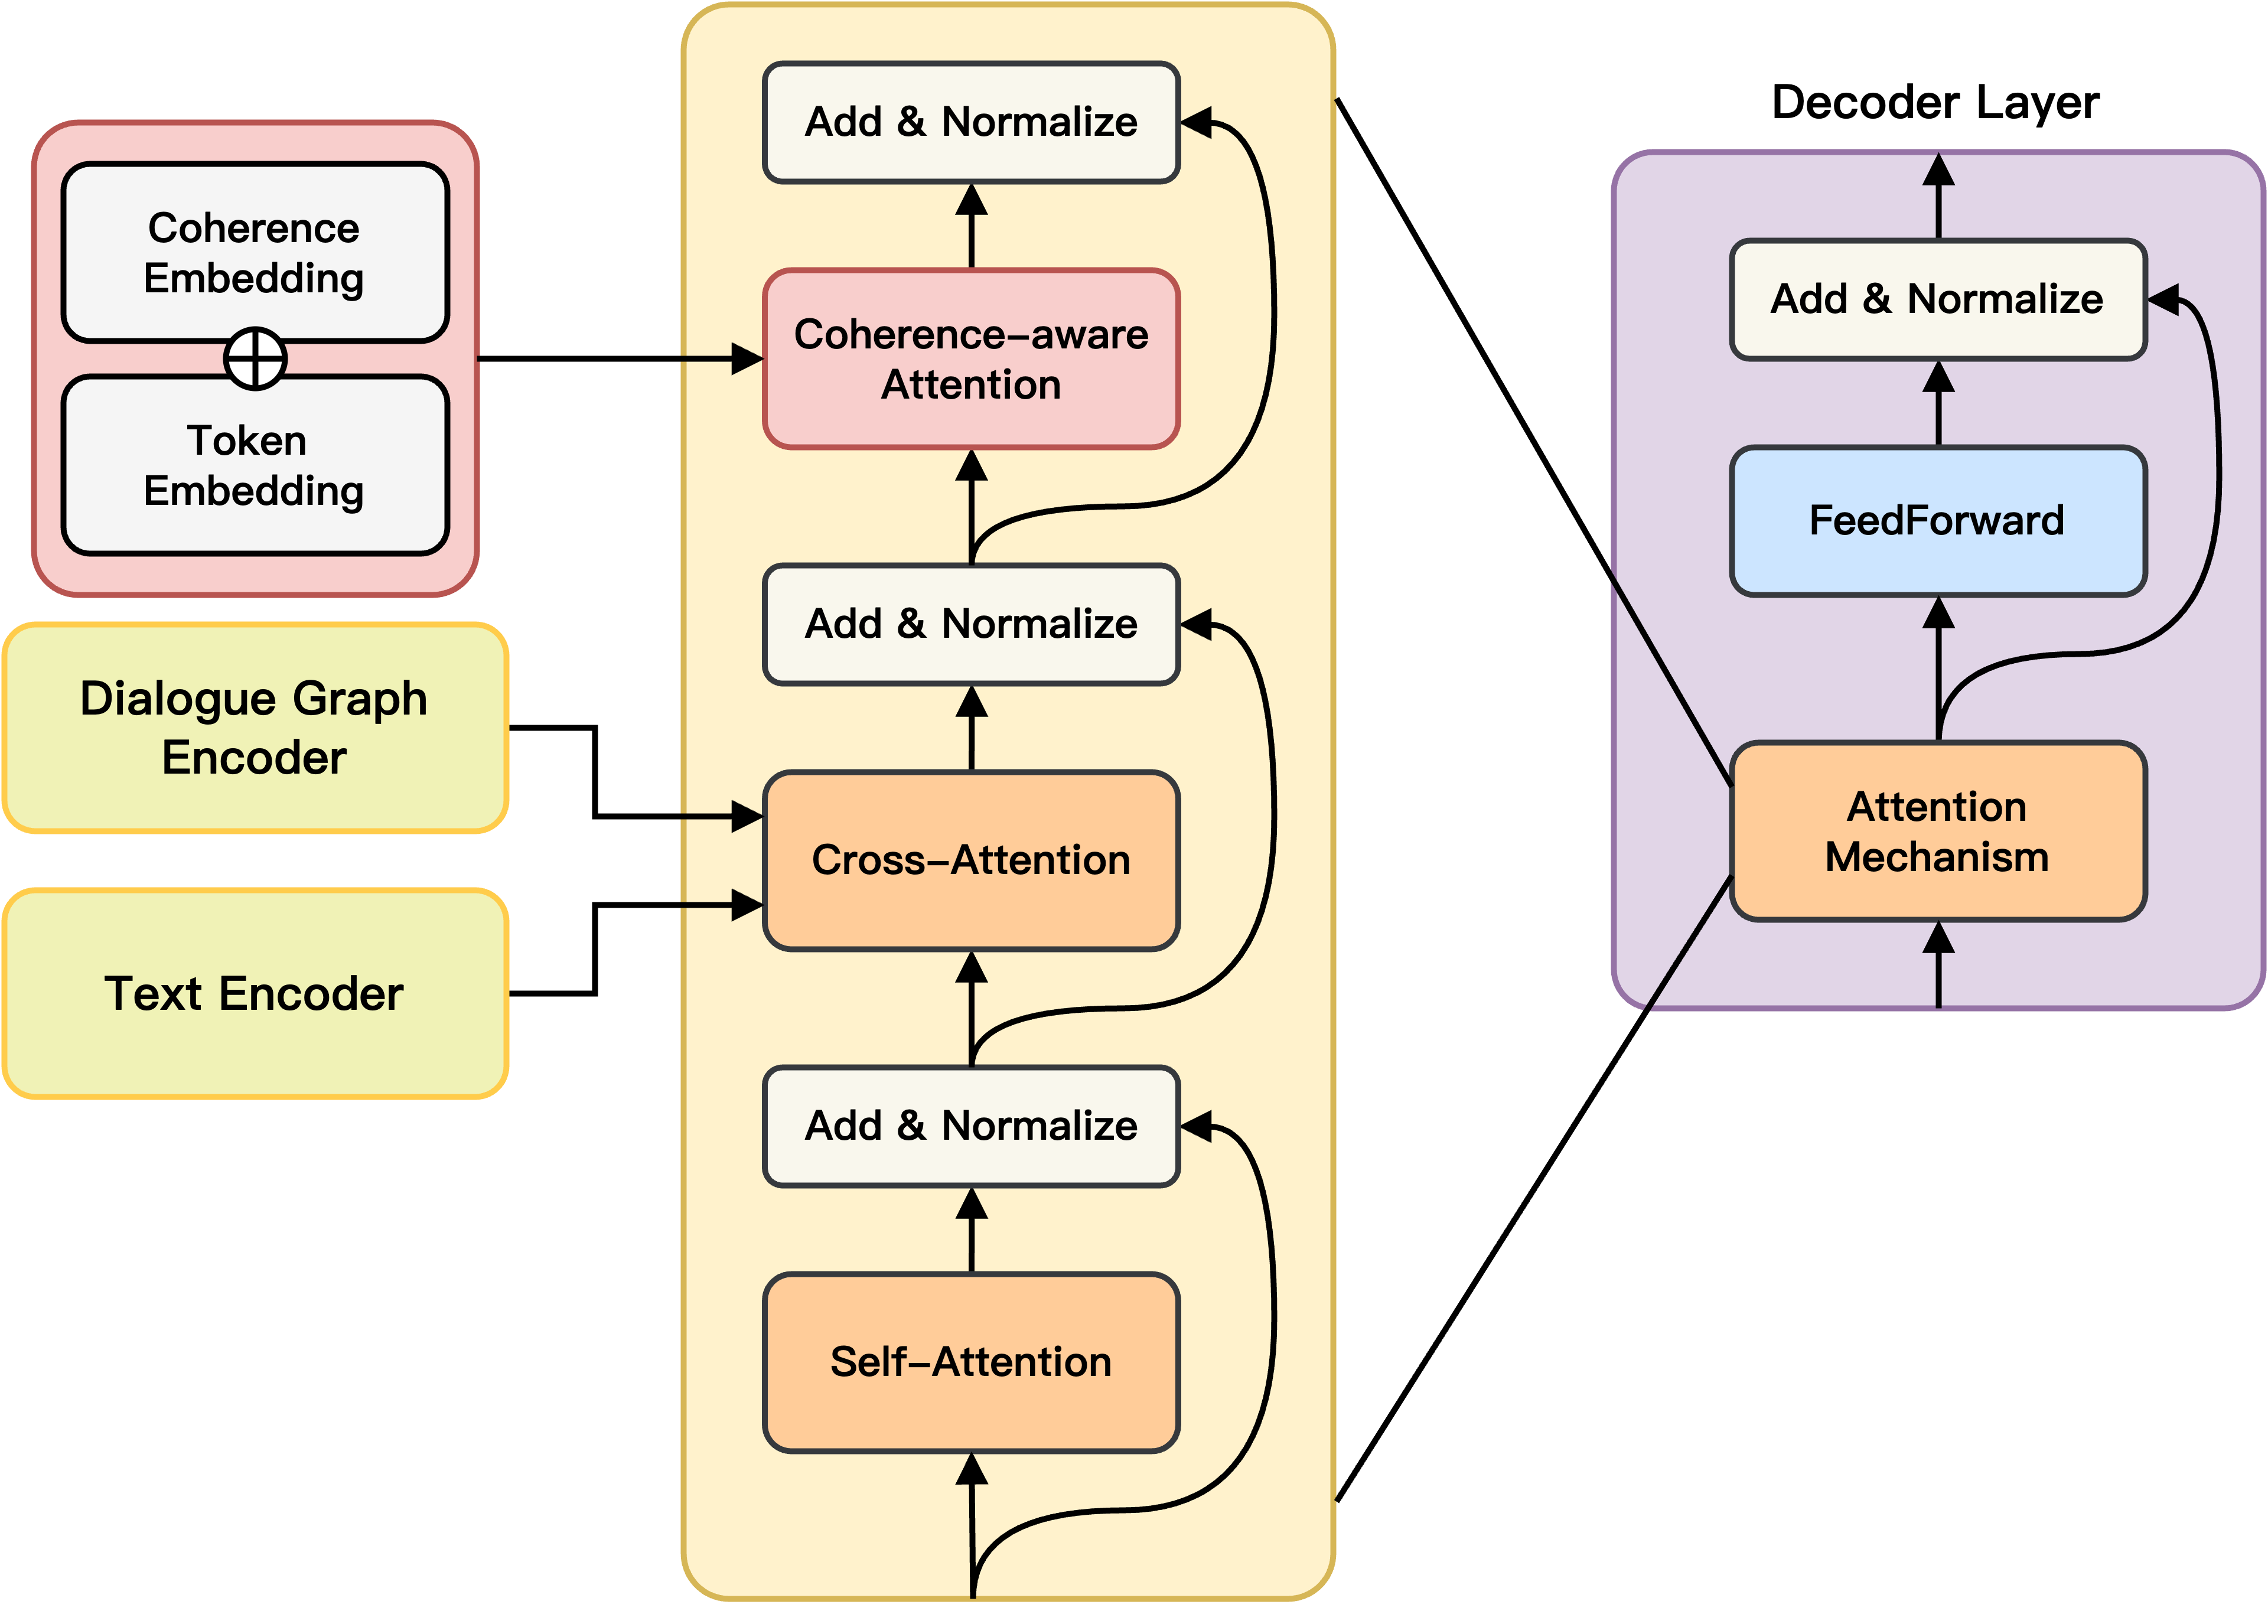
\includegraphics[width=1.00\textwidth]{./context/methodology/images/coherence-aware_attention.png}
    \caption{The visualizations of Coherence-aware Attention. We first compute the cross-attention between the encoder and decoder information. Then, we concatenate the coherence embedding and token embedding of the specified response type with this cross-attention result and perform coherence-aware attention to enrich the discourse information.}
    \label{fig:coherence-aware_attention}
\end{figure}

Finally, to enable the generator to better consider both persona-aware and coherence-aware context information during generation, we are inspired by \cite{huang-etal-2023-paa}. We fuse the decoder hidden states that consider the text encoder information with those that consider the dialogue graph encoder through a Dynamic Weighted Aggregation mechanism. Specifically, we compute a weight $w_{\text{TextEnc}}$ using a sigmoid function over the concatenated hidden states from both encoders (Eq. \ref{eq:dynamic_weighted_aggregation_weight}). Using this weight, we create masked versions of the encoder outputs based on a threshold hyperparameter $\tau$ to control the proportion of persona-aware and coherence-aware information to be considered (Eq. \ref{eq:dynamic_weighted_aggregation_weighting} and \ref{eq:dynamic_weighted_aggregation_mask}). The final output of the generator $O_{\text{Generator}}$ is obtained by adding a residual connection of the original encoder hidden states to the aggregated hidden states, enhancing the coherence and personalization of the generated responses. The detailed formulas are provided in the following equations:

\begin{equation} \label{eq:dynamic_weighted_aggregation_weight}
    w_{\text{TextEnc}} = \sigma(\text{MLP}([H_{\text{TextEnc}} \parallel H_{\text{GraphEnc}}]))
\end{equation}

\begin{equation} \label{eq:dynamic_weighted_aggregation_weighting}
    \begin{aligned}
        O_{\text{TextEnc}} &= w_{\text{TextEnc}} \cdot H_{\text{TextEnc}}, \\
        O_{\text{GraphEnc}} &= (1 - w_{\text{TextEnc}}) \cdot H_{\text{GraphEnc}}
    \end{aligned}
\end{equation}

\begin{equation} \label{eq:dynamic_weighted_aggregation_mask}
    \begin{aligned}
        m_{\text{TextEnc}} &= \mathbb{M}(w_{TextEnc} > \tau), \\
        m_{\text{GraphEnc}} &= \mathbb{M}(1 - w_{TextEnc} > \tau)
    \end{aligned}
\end{equation}

\begin{equation}
    \begin{aligned}
        \hat{O}_{\text{TextEnc}} &= m_{\text{TextEnc}} \odot O_{\text{TextEnc}}, \\
        \hat{O}_{\text{GraphEnc}} &= m_{\text{GraphEnc}} \odot O_{\text{GraphEnc}}, \\
        H_{\text{Enc}} &= \hat{O}_{\text{TextEnc}} + \hat{O}_{\text{GraphEnc}}
    \end{aligned}
\end{equation}

\begin{equation} \label{eq:dynamic_weighted_aggregation_output}
    \begin{aligned}
        H_{\text{residual}} &= H_{\text{TextEnc}} + H_{\text{GraphEnc}}, \\
        O_{\text{Generator}} &= H_{\text{Enc}} + H_{\text{residual}}
    \end{aligned}
\end{equation}

For personalized response generation, we use a language modeling task to compute the probability distribution over the vocabulary for generating the next word given the current context. The language modeling loss, typically implemented as the negative log-likelihood loss, is computed between the predicted probability distribution and the actual next word in the training data. This encourages the model to generate responses that are not only contextually appropriate but also aligned with the persona. The loss function can be formally defined as:

\begin{equation}
    \mathcal{L}_{\text{LM}} = - \sum_{t=1}^{T} \log P(y_t | y_{<t}, O_{\text{Generator}})
\end{equation}

By minimizing this loss function, the model learns to produce fluent and personalized responses that are coherent with the dialogue history and consistent with the persona.

% ------------------------------------------------
\EndChapter
% ------------------------------------------------


% Experiment chapter
% ------------------------------------------------
\StartChapter{Experiment}{chapter:experiment}
% ------------------------------------------------
This chapter presents an evaluation of our proposed methods for personalized dialogue generation. We conducted experiments on the ConvAI2 dataset. Our approach surpasses previous methods in multiple evaluative aspects of response generation, showcasing superior results in personalized dialogue generation.

\section{Datasets}
ConvAI2 \cite{dinan-etal-2019-convai2} is a chit-chat dataset based on PersonaChat \cite{zhang-etal-2018-personalizing}. The dataset comprises 17,878 and 1,000 multi-turn dialogues for the training and development sets, respectively, with a total of 131,438 and 7,801 utterances. It features 1,155 and 100 unique persona descriptions for the training and development sets, respectively. Each conversation participant who are assigned at least five persona descriptions, which are selected from these unique personas. Examples of the dialogue can be seen in Table \ref{table:convai2-example}.

\section{Baselines}
For comparison, we have selected the following baselines: (1) \textbf{Personalized Dialogue Generation methods}: We compare our approach with established text-description-based personalized models such as BOB \cite{song-etal-2021-bob}, LMEDR \cite{chen-etal-2023-memorize}, and PAA \cite{huang-etal-2023-paa}, which are recognized for their strong performance. (2) \textbf{General Dialogue Generation methods}: To ensure a fair evaluation, we include PLATO \cite{bao-etal-2020-plato} and DialoGPT \cite{zhang-etal-2019-dialogpt}. For PLATO, following the original publication's methodology, we prepend the persona descriptions as part of the knowledge to the entire context during inference. For DialoGPT, we adopt a post-processing approach as suggested by \cite{zhou-etal-2023-simoap}. We first generate multiple responses as candidates from DialoGPT for the same context and then select the response that is most consistent with the persona and most relevant to the context as the final output. (3) \textbf{Large Language Models (LLMs)}: We also test the ability of LLMs, specifically GPT-4, in personalized response generation, which utilizes prompting technologies. The prompt can be seen in Figure \ref{fig:llm_inference_prompt}.

% ----------------------------------------------
% Table: ConvAI2 Dataset Example
% ----------------------------------------------

\begin{table}[ht]
\centering
\def\arraystretch{1.4}%
\begin{tabular}{|p{7cm}|p{7cm}|}
\hline

\rowcolor[RGB]{204,217,245}
\multicolumn{1}{|c|}{\textbf{PERSON 1's Persona}} & \multicolumn{1}{|c|}{\textbf{PERSON 2's Persona}} \\
\hline
I like to ski. & I am an artist. \\
My wife does not like me anymore. & I have four children. \\
I have went to Mexico 4 times this year. & I recently got a cat. \\
I hate Mexican food. & I enjoy walking for exercise. \\
I like to eat cheetos. & I love watching Game of Thrones. \\
\hline

\rowcolor[RGB]{204,217,245}
\multicolumn{2}{|c|}{\textbf{Dialogue}} \\
\hline

\multicolumn{2}{|p{14cm}|}{[PERSON 1:] Hi} \\
\multicolumn{2}{|p{14cm}|}{[PERSON 2:] Hello ! How are you today?} \\
\multicolumn{2}{|p{14cm}|}{[PERSON 1:] I am good thank you , how are you.} \\
\multicolumn{2}{|p{14cm}|}{[PERSON 2:] Great, thanks ! My children and I were just about to watch Game of Thrones.} \\
\multicolumn{2}{|p{14cm}|}{[PERSON 1:] Nice! How old are your children?} \\
\multicolumn{2}{|p{14cm}|}{[PERSON 2:] I have four that range in age from 10 to 21. You?} \\
\multicolumn{2}{|p{14cm}|}{[PERSON 1:] I do not have children at the moment.} \\
\multicolumn{2}{|p{14cm}|}{[PERSON 2:] That just means you get to keep all the popcorn for yourself.} \\
\multicolumn{2}{|p{14cm}|}{[PERSON 1:] And Cheetos at the moment!} \\
\multicolumn{2}{|p{14cm}|}{[PERSON 2:] Good choice. Do you watch Game of Thrones?} \\
\multicolumn{2}{|p{14cm}|}{[PERSON 1:] No, I do not have much time for TV.} \\
\multicolumn{2}{|p{14cm}|}{[PERSON 2:] I usually spend my time painting. But, I love the show.} \\

\hline
\end{tabular}
\caption{Example dialogue from the ConvAI2 dataset. During training, the model acts as a conversational agent, playing the role of one of the participants to generate personalized responses.}
\label{table:convai2-example}
\end{table}

\section{Implementation Details}
The \textbf{MUDI} is mainly implemented in PyTorch. Our backbone Generator is BART-large\footnote[2]{https://huggingface.co/facebook/bart-large}. For Generator training, we train it using a batch size of 4 on 1 NVIDIA A100 80GB
GPU via the AdamW optimizer with a learning rate of \(5 \times 10^{-6}\) and a
weight decay of 0.01. For the Dialogue Graph Encoder training, it is conducted on a single NVIDIA RTX 4090 GPU using a batch size of 512. The training also employs the AdamW optimizer, but with a learning rate of \(2 \times 10^{-5}\) and the same weight decay of 0.01. In the Dialogue Graph Encoder, we initially employ the SBERT model "all-mpnet-base-v2"\footnote[3]{https://huggingface.co/sentence-transformers/all-mpnet-base-v2} to encode both the utterances and persona sentences, thereby initializing the node embeddings. We construct the Dialogue Graph by keeping the 3-hop neighbors. The model employs a 2-layer GNN with 4 multi-heads and a hidden dimension of 512. The weights for the different tasks are as follows: the weight of the Coherence Relation Classification task is 1.5, the weight of both types of Next Response Type Prediction tasks is 1.5, and the weight of the Link Prediction task is 1.2. For training the generator, we retain the most recent 5 turns of dialogue as historical context and choose the top-3 predicted response types for the prompt. We set \(\tau = 0.2\) for the Dynamic Weighted Aggregation.

\InsertFigure
[scale=0.46,
caption={The prompt of LLM inference on Personalized Dialogue Generation task.},
label={fig:llm_inference_prompt}
]
{./context/experiment/images/llm_inference_prompt.png}

\section{Evaluation Metrics}
\subsection{Automatic Metrics}
We assess the quality of dialogue responses from four perspectives: 

(1) \textbf{Text-similarity}: To evaluate the similarity between the generated responses and the ground-truth responses, we employ BLEU \cite{papineni-etal-2002-bleu} and ROUGE \cite{lin-2004-rouge} metrics, which focus on the word overlap level. Additionally, we utilize BERTScore \cite{zhang-etal-2020-bert-score}, which measures the semantic similarity between generated responses and ground-truth using contextual embeddings from BERT. This helps capture nuances that traditional overlap-based metrics might miss.

(2) \textbf{Diversity}: We assess the diversity and informativeness of the generated responses at token, sentence, and corpus levels. We utilize Distinct-n (Dist-$n$) metrics \cite{li-etal-2016-diversity} to measure the proportion of unique n-grams (n=1) relative to the total number of n-grams in the generated responses. Additionally, we employ Entropy-n (Ent-$n$) \cite{zhang-etal-2018-generating} to evaluate the uncertainty or randomness of the distribution of n-grams (n=1) in the generated text. We also calculate the Unique Sentence Ratio (USR) \cite{li-etal-2020-generate}, which quantifies text diversity by measuring the proportion of unique sentences among all predicted responses.

(3) \textbf{Coherence}: Previous studies often omit explicit evaluations of Coherence, assuming that Fluency can also measure the coherence of dialogues. However, this approach does not directly account for the coherence of generated responses with the context and query, an aspect often presumed to be covered by fluency. To measure this unexplored dimension, our research incorporates specific coherence metrics to provide a more accurate and holistic assessment of response quality. Specifically, we employ several metrics. Firstly, we use QuantiDCE \cite{ye-etal-2021-towards-quantifiable} and DEAM \cite{ghazarian-etal-2022-deam}, which are state-of-the-art metrics in dialogue coherence evaluation. These metrics assess both how logically the responses align with the preceding query or the entire context within the dialogue, and how well the utterances in a conversation are unified, leading to a consistent and coherent interaction. Additionally, we utilize BARTScore \cite{yuan-etal-2021-bartscore} to measure coherence under the faithfulness setting discussed in the paper.

(4) \textbf{Personalization}: To assess the personalization of the generated responses, we first measure the alignment between the persona and responses. First, we apply Consistency Score (C.Score) \cite{madotto-etal-2019-personalizing}, which leverages a NLI model to predict consistency between response and persona. Additionally, we utilize the BARTScore \cite{yuan-etal-2021-bartscore}, which provides a method to calculate the semantic overlaps between texts. Specifically, we compute: (a) Precision (persona → response): This measures how closely the generated responses adhere to the input persona, reflecting the degree to which the model captures persona-specific attributes in the response. (b) Recall (response → persona): This assesses whether all aspects of the persona are sufficiently covered by the responses, indicating the comprehensiveness of the persona information in the generated text. we report the F1 Score is then calculated from these Precision and Recall scores to provide a balanced measure of personalization, capturing both the accuracy and completeness of the generated responses in reflecting the specified persona.

Moreover, to better assess whether the generated responses accurately incorporate important features from the persona or the query, we utilize Large Language Models (LLMs)\footnote[4]{https://huggingface.co/meta-llama/Meta-Llama-3-70B-Instruct} to identify key terms (features) from these persona descriptions or dialogue utterances. We then employ a NLI model to calculate the Feature Coverage Ratio (FCR), ensuring that critical features are effectively represented in the responses. The example of the feature-annotated table mentioned earlier is shown in Table \ref{table:fcr-feature-annotated-example}.

\begin{table}[H]
\centering
\def\arraystretch{1.2}%
\begin{tabular}{|l|c|}
\hline

\rowcolor[RGB]{204,217,245}
\multicolumn{1}{|c|}{\textbf{Persona description}} & \textbf{Features} \\
\hline

I read twenty books a year. & read books, twenty books a year   \\
\hline

I'm a stunt double as my second job. & stunt double, second job \\
\hline

I only eat kosher. & only eat kosher \\
\hline

I was raised in a single parent household. & single parent household \\
\hline

\rowcolor[RGB]{204,217,245}
\multicolumn{1}{|c|}{\textbf{Utterance}} & \textbf{Features} \\
\hline

Oh wow. All i've is a dog. That's enough for me. & having a dog  \\
\hline

I am good, I just got off work and tired, I have two jobs. & got off work, two jobs, tired \\
\hline

But a good movie is always good. & good movie \\
\hline

\end{tabular}
\caption{Examples of feature annotations used for calculating the Feature Coverage Ratio (FCR). All personas and queries in the dialogue have been annotated.}
\label{table:fcr-feature-annotated-example}
\end{table}

\section{Main Results}
Apart from DialoGPT, we use the context of the most recent 5 turns as dialogue history. After testing, we found that DialoGPT starts to talk nonsense when given more than 2 turns of context. Therefore, for DialoGPT, we only use the most recent 2 turns.

In Table \ref{table:text-similarity}, we report experimental results on Text Similarity evaluation. Our method offers better BLEU, ROUGE, and BERTScore compared with baseline methods. Specifically, MUDI's BLEU-1, ROUGE-1, and ROUGE-L scores reach 18.19, 17.10, and 16.13, respectively, outperforming existing methods by 1.64, 3.57, and 3.45. As shown in Table \ref{table:text-diversity}, we report the Diversity evaluation. MUDI's USR is 1.0, indicating that it can generate completely unique responses under different queries and personas. Additionally, we achieved the second-highest scores in Ent-1 and Dist-1. Upon examining the outputs from PLATO, we found that they often generate shorter sentences, such as 'me to!!'. Shorter sentences tend to inflate certain metrics, like Dist-1, because they typically involve less repetition of words within a single response, leading to high distinct scores. This suggests that while our method ranks second, it could provide more substantial and contextually rich responses compared to PLATO. Furthermore, our approach achieves the highest scores among all Persona-based dialogue generation methods and significantly surpasses other baselines in Dist-1, outperforming them by 7.95. This performance establishes our method could generate varied and engaging responses.

In addition, Table \ref{table:coherence} presents the results of the Coherence evaluation. Compared to other persona-based methods, MUDI has made significant progress in QuantiDCE, DEAM, and BARTScore, particularly in assessing the coherence between the query and response (left-side scores). This indicates that our approach indeed enables the model to generate responses with enhanced local coherence. Furthermore, MUDI also achieves excellent results in global coherence, which evaluates the coherence between the entire dialogue context and the response (right-side scores).

Finally, Table \ref{table:personalization} presents the results of evaluating Personalization and Feature Coverage. PAA significantly outperforms other methods in scores for Personalization and FCR$_p$. Upon further examination, we discovered that this is because PAA frequently generates sentences that are exact restatements of the persona description, often ignoring the relevance to the query. As a result, its high scores in Personalization can be attributed to this tendency. Excluding the special case of PAA, MUDI achieves excellent results in Personalization compared to other methods. Combined with the previously discussed results from the Coherence evaluation (Table \ref{table:personalization}), this demonstrates that our approach successfully balances discourse relations and persona. It generates responses that effectively consider both aspects simultaneously. Furthermore, our model achieves comparable scores in the Coherence evaluation compared to DialoGPT, which focuses on general dialogue generation.

In evaluating powerful LLMs like GPT-4, we find that they excel at generating lengthy responses and maintaining coherence between questions and dialogue context. Consequently, GPT-4 stands out in Coherence evaluation, scores highly in Ent-1, and performs well in FCR$_q$. However, this also results in a lower overlap with the ground-truth responses, leading to lower Text Similarity scores. Moreover, the longer sentences generated lead to a lower Dist-1 score. Another observation is that GPT-4 performs well in tasks related to Personalization, which confirms the robust capabilities of large-parameter LLMs. Additionally, when we provide LLMs with information on coherence relations, there is an observed improvement in FCR evaluations. This suggests that appropriate response type guidance can focus the LLM more on the important aspects of the questions, thus making it easier for the model to generate sentences that are relevant to the persona. However, previous research \cite{deshpande-etal-2023-toxicity} suggests that using LLMs for personalized dialogue generation can encounter biases in the generated content, which still requires careful consideration.

In summary, compared to existing methods, our approach MUDI not only significantly improves performance in Text Similarity scores but also excels at integrating discourse relations and persona information. This enables us to generate personalized responses that are not only rich in content and diverse but also encompass these aspects. Moreover, in Coherence evaluations, our method achieves scores comparable to those of state-of-the-art models specialized in open-domain dialogue generation.

% ----------------------------------------------
% Table 1: Text Similarity
% ----------------------------------------------

\begin{table}[H]
\centering
\def\arraystretch{1.3}%
\begin{tabular}{|c|c|c|c|c|c|c|}
\hline
\multicolumn{2}{|c|}{\multirow{2}{*}{\textbf{Model}}}  & \multicolumn{5}{c|}{\textbf{Text Similarity}} \\
\cline{3-7}

\multicolumn{2}{|c|}{} & BLEU-1 $\uparrow$ & BLEU-2 $\uparrow$ & ROUGE-1 $\uparrow$ & ROUGE-L $\uparrow$ & BERTScore $\uparrow$ \\
\hhline{|=======|}

\rowcolor[RGB]{242,164,100}
\multicolumn{7}{|c|}{\textbf{Large Language Model (Prompting)}} \\
\hhline{|=======|}

\multicolumn{2}{|c|}{\textbf{GPT-4}} &7.47 &2.40 &13.52 &11.06 &84.05 \\ 
\hhline{|=======|}

\rowcolor{yellow}
\multicolumn{7}{|c|}{\textbf{General Dialogue Generation}} \\
\hhline{|=======|}

\multicolumn{2}{|c|}{\textbf{DialoGPT}} &7.34	&1.54 &9.46 &8.41 &83.31 \\ 
\hline

\multirow{2}{*}{\textbf{PLATO}} & w/ persona &4.35	&1.01 &4.88 &4.80 &82.77 \\ 
\cline{2-7}

\multirow{2}{*}{\textbf{}} & w/o persona  &6.82 &1.86 &4.99 &4.77 &81.44 \\ 
\hhline{|=======|}

\rowcolor[RGB]{204,217,245}
\multicolumn{7}{|c|}{\textbf{Persona-based Dialogue Generation}} \\
\hhline{|=======|}

\multicolumn{2}{|c|}{\textbf{BoB}} &15.30 &5.39 &13.21 &12.48 &83.77 \\ 
\hline

% \multicolumn{2}{|c|}{\textbf{P$^{2}$BOT}} &- &- &- &- &- \\ 
% \hline

\multicolumn{2}{|c|}{\textbf{LMEDR}}		&15.47	&5.83	&13.28	&12.26	&85.00 \\ 
\hline

\multicolumn{2}{|c|}{\textbf{PAA}}          &\underline{16.55}    &6.28    &13.53 
&12.68    &84.42   \\
\hline

\multirow{3}{*}{\textbf{\begin{tabular}{@{}c@{}}MUDI \\ (ours)\end{tabular}}} &SP\textsubscript{$\tau=0.2$}	&15.14	&6.43	&14.87	&13.87	&85.07	\\
\cline{2-7}

\multirow{3}{*}{} &Emb\textsubscript{$\tau=0.2$}   &\underline{16.55}    &\underline{7.34}	&\textbf{\textcolor{red}{17.10}}	&\textbf{\textcolor{red}{16.13}}	&\underline{85.42}	\\
\cline{2-7}

\multirow{3}{*}{} &SP+Emb\textsubscript{$\tau=0.2$}   &\textbf{\textcolor{red}{18.19}} &\textbf{\textcolor{red}{7.77}}	&\underline{16.59}	&\underline{15.46}	&\textbf{\textcolor{red}{85.53}} \\
\hline
\end{tabular}
\caption{Automatic evaluation results on ConvAI2 dataset over our implemented approach. The best results in each column are in bold, while the second is underlined.}
\label{table:text-similarity}
\end{table}

% ----------------------------------------------
% Table 2: Diversity
% ----------------------------------------------

\begin{table}[H]
\centering
\def\arraystretch{1.3}%
\begin{tabular}{|c|c|c|c|c|}
\hline
\multicolumn{2}{|c|}{\multirow{2}{*}{\textbf{Model}}}  &\multicolumn{3}{c|}{\textbf{Diversity}}\\
\cline{3-5}

\multicolumn{2}{|c|}{} &Ent-1 $\uparrow$ &Dist-1 $\uparrow$ &USR $\uparrow$ \\
\hhline{|=====|}

\rowcolor[RGB]{242,164,100}
\multicolumn{5}{|c|}{\textbf{Large Language Model (Prompting)}} \\
\hhline{|=====|}

\multicolumn{2}{|c|}{\textbf{GPT-4}} &9.40 &16.09 &1.00 \\ 
\hhline{|=====|}

\rowcolor{yellow}
\multicolumn{5}{|c|}{\textbf{General Dialogue Generation}} \\
\hhline{|=====|}

\multicolumn{2}{|c|}{\textbf{DialoGPT}} &\textbf{\textcolor{red}{9.05}} &36.84 &\underline{0.99} \\ 
\hline

\multirow{2}{*}{\textbf{PLATO}} & w/ persona &4.67 &\textbf{\textcolor{red}{58.18}} &0.61 \\ 
\cline{2-5}

\multirow{2}{*}{\textbf{}} & w/o persona &6.73 &43.34 &0.85 \\ 
\hhline{|=====|}

\rowcolor[RGB]{204,217,245}
\multicolumn{5}{|c|}{\textbf{Persona-based Dialogue Generation}} \\
\hhline{|=====|}


\multicolumn{2}{|c|}{\textbf{BoB}} &7.89 &41.75 &\underline{0.99} \\ 
\hline

% \multicolumn{2}{|c|}{\textbf{P$^{2}$BOT}} &- &- &- \\ 
% \hline

\multicolumn{2}{|c|}{\textbf{LMEDR}}  &7.14	&43.08	&0.94\\ 
\hline

\multicolumn{2}{|c|}{\textbf{PAA}}    &6.66	&40.27  &0.87 \\
\hline

\multirow{3}{*}{\textbf{\begin{tabular}{@{}c@{}}MUDI \\ (ours)\end{tabular}}} &SP\textsubscript{$\tau=0.2$}	&\underline{8.13}		&46.76	&\textbf{\textcolor{red}{1.00}}\\
\cline{2-5}

\multirow{3}{*}{} &Emb\textsubscript{$\tau=0.2$}   &7.65	&\underline{51.03}	&\textbf{\textcolor{red}{1.00}}\\
\cline{2-5}

\multirow{3}{*}{} &SP+Emb\textsubscript{$\tau=0.2$} 	&7.66	&47.68  &\textbf{\textcolor{red}{1.00}}\\
\hline
\end{tabular}
\caption{Automatic evaluation results for diversity tested on ConvAI2 dataset over our implemented approach. The best results in each column are in bold, while the second is underlined.}
\label{table:text-diversity}
\end{table}

% ----------------------------------------------
% Table 3: Coherence 
% ----------------------------------------------

\begin{table}[H]
\centering
\def\arraystretch{1.3}%
\begin{tabular}{|c|c|c|c|c|}
\hline
\multicolumn{2}{|c|}{\multirow{2}{*}{\textbf{Model}}}  & \multicolumn{3}{c|}{\textbf{Coherence}} \\
\cline{3-5}

\multicolumn{2}{|c|}{} & QuantiDCE $\uparrow$ & DEAM $\uparrow$ & BARTScore$_{q \rightarrow r, c \rightarrow r}$ $\downarrow$ \\
\hline

\multicolumn{2}{|c|}{\textbf{GOLD}}          &3.19 / 2.83    &0.64 / 0.85    &5.74 / 5.70   \\
\hhline{|=====|}

\rowcolor[RGB]{242,164,100}
\multicolumn{5}{|c|}{\textbf{Large Language Model (Prompting)}} \\
\hhline{|=====|}

\multirow{2}{*}{\textbf{GPT-4}} & w/ coherence relations  &3.40 / 2.91 &0.77 / 0.95 &4.27 / 3.74 \\ 
\cline{2-5}
\multirow{2}{*}{\textbf{}} & w/o coherence relations  &3.41 / 2.92 &0.87 / 0.96 &4.24 / 3.73 \\ 

\hhline{|=====|}

\rowcolor{yellow}
\multicolumn{5}{|c|}{\textbf{General Dialogue Generation}} \\
\hhline{|=====|}

\multicolumn{2}{|c|}{\textbf{DialoGPT}} &\textbf{\textcolor{red}{3.23}} / 2.79 &\textbf{\textcolor{red}{0.70}} / \textbf{\textcolor{red}{0.88}} &5.12 / 5.19 \\ 
\hline

% \multirow{2}{*}{\textbf{PLATO}} & w/ persona &3.32 / 3.43	&0.22 / 0.75 &6.42 / 6.63 \\ 
\multirow{2}{*}{\textbf{PLATO}} & w/ persona &1.68 / 1.57	&0.22 / 0.75 &6.42 / 6.63 \\ 
\cline{2-5}

\multirow{2}{*}{\textbf{}} & w/o persona  &1.87 / 1.77 &0.25 / 0.74 &5.83 / 5.80 \\ 
\hhline{|=====|}

\rowcolor[RGB]{204,217,245}
\multicolumn{5}{|c|}{\textbf{Persona-based Dialogue Generation}} \\
\hhline{|=====|}

\multicolumn{2}{|c|}{\textbf{BoB}} &2.99 / 2.76 &0.39 / 0.86 &5.82 / 5.92 \\ 
\hline

% \multicolumn{2}{|c|}{\textbf{P$^{2}$BOT}} &- &- &- \\ 
% \hline

\multicolumn{2}{|c|}{\textbf{LMEDR}}		&2.89 / 2.90	&0.43 / 0.78	&5.32 / 4.99  \\ 
\hline

\multicolumn{2}{|c|}{\textbf{PAA}}           &2.70 / \underline{2.93}    &0.56 / 0.83    &5.17 / \underline{4.62}   \\
\hline

\multirow{3}{*}{\textbf{\begin{tabular}{@{}c@{}}MUDI \\ (ours)\end{tabular}}} &SP\textsubscript{$\tau=0.2$}	&3.05 / 2.84	&0.63 / 0.85	&\underline{4.67} / \textbf{\textcolor{red}{4.61}}	\\
\cline{2-5}

\multirow{3}{*}{} &Emb\textsubscript{$\tau=0.2$}   &\textbf{\textcolor{red}{3.23}} / \textbf{\textcolor{red}{2.94}}    &0.56 / 0.82	&4.80 / 4.83 \\
\cline{2-5}

\multirow{3}{*}{} &SP+Emb\textsubscript{$\tau=0.2$}   &\underline{3.21} / 2.92	&\underline{0.64} / \underline{0.86}	&\textbf{\textcolor{red}{4.66}} / 4.66	\\
\hline
\end{tabular}
\caption{Automatic evaluation results for coherence tested on the ConvAI2 dataset. The best results in each column are in bold, while the second-best results are underlined. The score on the left considers only the local coherence between the query and the response, while the score on the right takes into account the global coherence between the entire dialogue and the response.}
\label{table:coherence}
\end{table}

% ----------------------------------------------
% Table 4: Personalization & Feature Coverage
% ----------------------------------------------

\begin{table}[H]
\centering
\def\arraystretch{1.3}%
\begin{tabular}{|c|c|c|c|c|c|}
\hline
\multicolumn{2}{|c|}{\multirow{2}{*}{\textbf{Model}}}  &\multicolumn{2}{c|}{\textbf{Personalization}} &\multicolumn{2}{c|}{\textbf{Feature Coverage}}\\
\cline{3-6}

\multicolumn{2}{|c|}{} &C.Score $\uparrow$ &BARTScore$_{p \leftrightarrow r}$ $\downarrow$ &FCR$_{q}$ $\uparrow$ &FCR$_{p}$ $\uparrow$ \\
\hline

\multicolumn{2}{|c|}{\textbf{GOLD}}      &4.10   &5.68 &7.69 &4.52 \\
\hhline{|======|}

\rowcolor[RGB]{242,164,100}
\multicolumn{6}{|c|}{\textbf{Large Language Model (Prompting)}} \\
\hhline{|======|}

\multirow{2}{*}{\textbf{GPT-4}} & w/ coherence relations  &29.47 &4.33 &21.62 &27.12 \\ 
\cline{2-6}
\multirow{2}{*}{\textbf{}} & w/o coherence relations  &28.90 &4.07 &9.77 &5.72 \\ 
\hhline{|======|}

\rowcolor{yellow}
\multicolumn{6}{|c|}{\textbf{General Dialogue Generation}} \\
\hhline{|======|}

\multicolumn{2}{|c|}{\textbf{DialoGPT}} &4.53 &5.39 &\textbf{\textcolor{red}{6.78}} &4.45  \\ 
\hline

\multirow{2}{*}{\textbf{PLATO}} & w/ persona &0.56 &6.06 &1.20 &0.92 \\ 
\cline{2-6}

\multirow{2}{*}{\textbf{}} & w/o persona  &0.18 &5.83 &3.23 &0.28 \\ 
\hhline{|======|}

\rowcolor[RGB]{204,217,245}
\multicolumn{6}{|c|}{\textbf{Persona-based Dialogue Generation}} \\
\hhline{|======|}

\multicolumn{2}{|c|}{\textbf{BoB}} &0.51 &5.52 &3.68 &0.42  \\ 
\hline

% \multicolumn{2}{|c|}{\textbf{P$^{2}$BOT}} &- &- &- &-  \\ 
% \hline

\multicolumn{2}{|c|}{\textbf{LMEDR}}		&7.38	&5.27 &4.63	 &6.99 \\ 
\hline


\multicolumn{2}{|c|}{\textbf{PAA}}       &\textbf{\textcolor{red}{15.19}}   &\textbf{\textcolor{red}{4.26}} &\underline{4.66}    &\textbf{\textcolor{red}{13.84}} \\
\hline

\multirow{3}{*}{\textbf{\begin{tabular}{@{}c@{}}MUDI \\ (ours)\end{tabular}}} &SP\textsubscript{$\tau=0.2$}	&\underline{11.87} &\underline{4.53} &\underline{4.66} &6.50	\\
\cline{2-6}

\multirow{3}{*}{} &Emb\textsubscript{$\tau=0.2$}   &9.70	&4.75 &4.36 &\underline{7.77} \\
\cline{2-6}

\multirow{3}{*}{} &SP+Emb\textsubscript{$\tau=0.2$}  &9.75	&4.76 &4.05 &5.01 \\
\hline
\end{tabular}
\caption{Automatic evaluation results for personalization and feature coverage tested on the  ConvAI2 dataset. The best results in each column are in bold, while the second-best results are underlined.}
\label{table:personalization}
\end{table}

% ----------------------------------------------
% Section: Analysis
% ----------------------------------------------

\section{Analysis}

\subsection{The Effect of Proposed DialogueGAT}
To validate the performance of the proposed DialogueGAT compared with existing GNN methods in Dialogue Graph modeling, we analyze results in the Next Response Type Prediction (NRTP) and Coherence Relations Classification tasks on the validation set. We compare DialogueGAT with GATv2. This comparison is illustrated in Figure \ref{fig:compare_gatv2_dialoguegat}. The experimental results demonstrate that DialogueGAT consistently outperforms GATv2 across all tasks in terms of Hits@5 scores, highlighting its enhanced capability to predict discourse relations (response types) from dialogue context information. Notably, in the Coherence Relations Classification (RC) task, DialogueGAT achieves significant improvements, showcasing its robustness in understanding context relationships. Additionally, the loss metrics further validate the efficiency of DialogueGAT; it registers lower loss values than GATv2 in both NRTP tasks, indicating superior model optimization and better fitting. The most pronounced difference is observed in the RC task, where the loss for DialogueGAT is markedly lower, emphasizing its exceptional performance in accurately classifying coherence relations. These findings suggest that DialogueGAT enhances prediction accuracy and effectively reduces error rates in discourse understanding.

\begin{figure}[H]
    \centering
    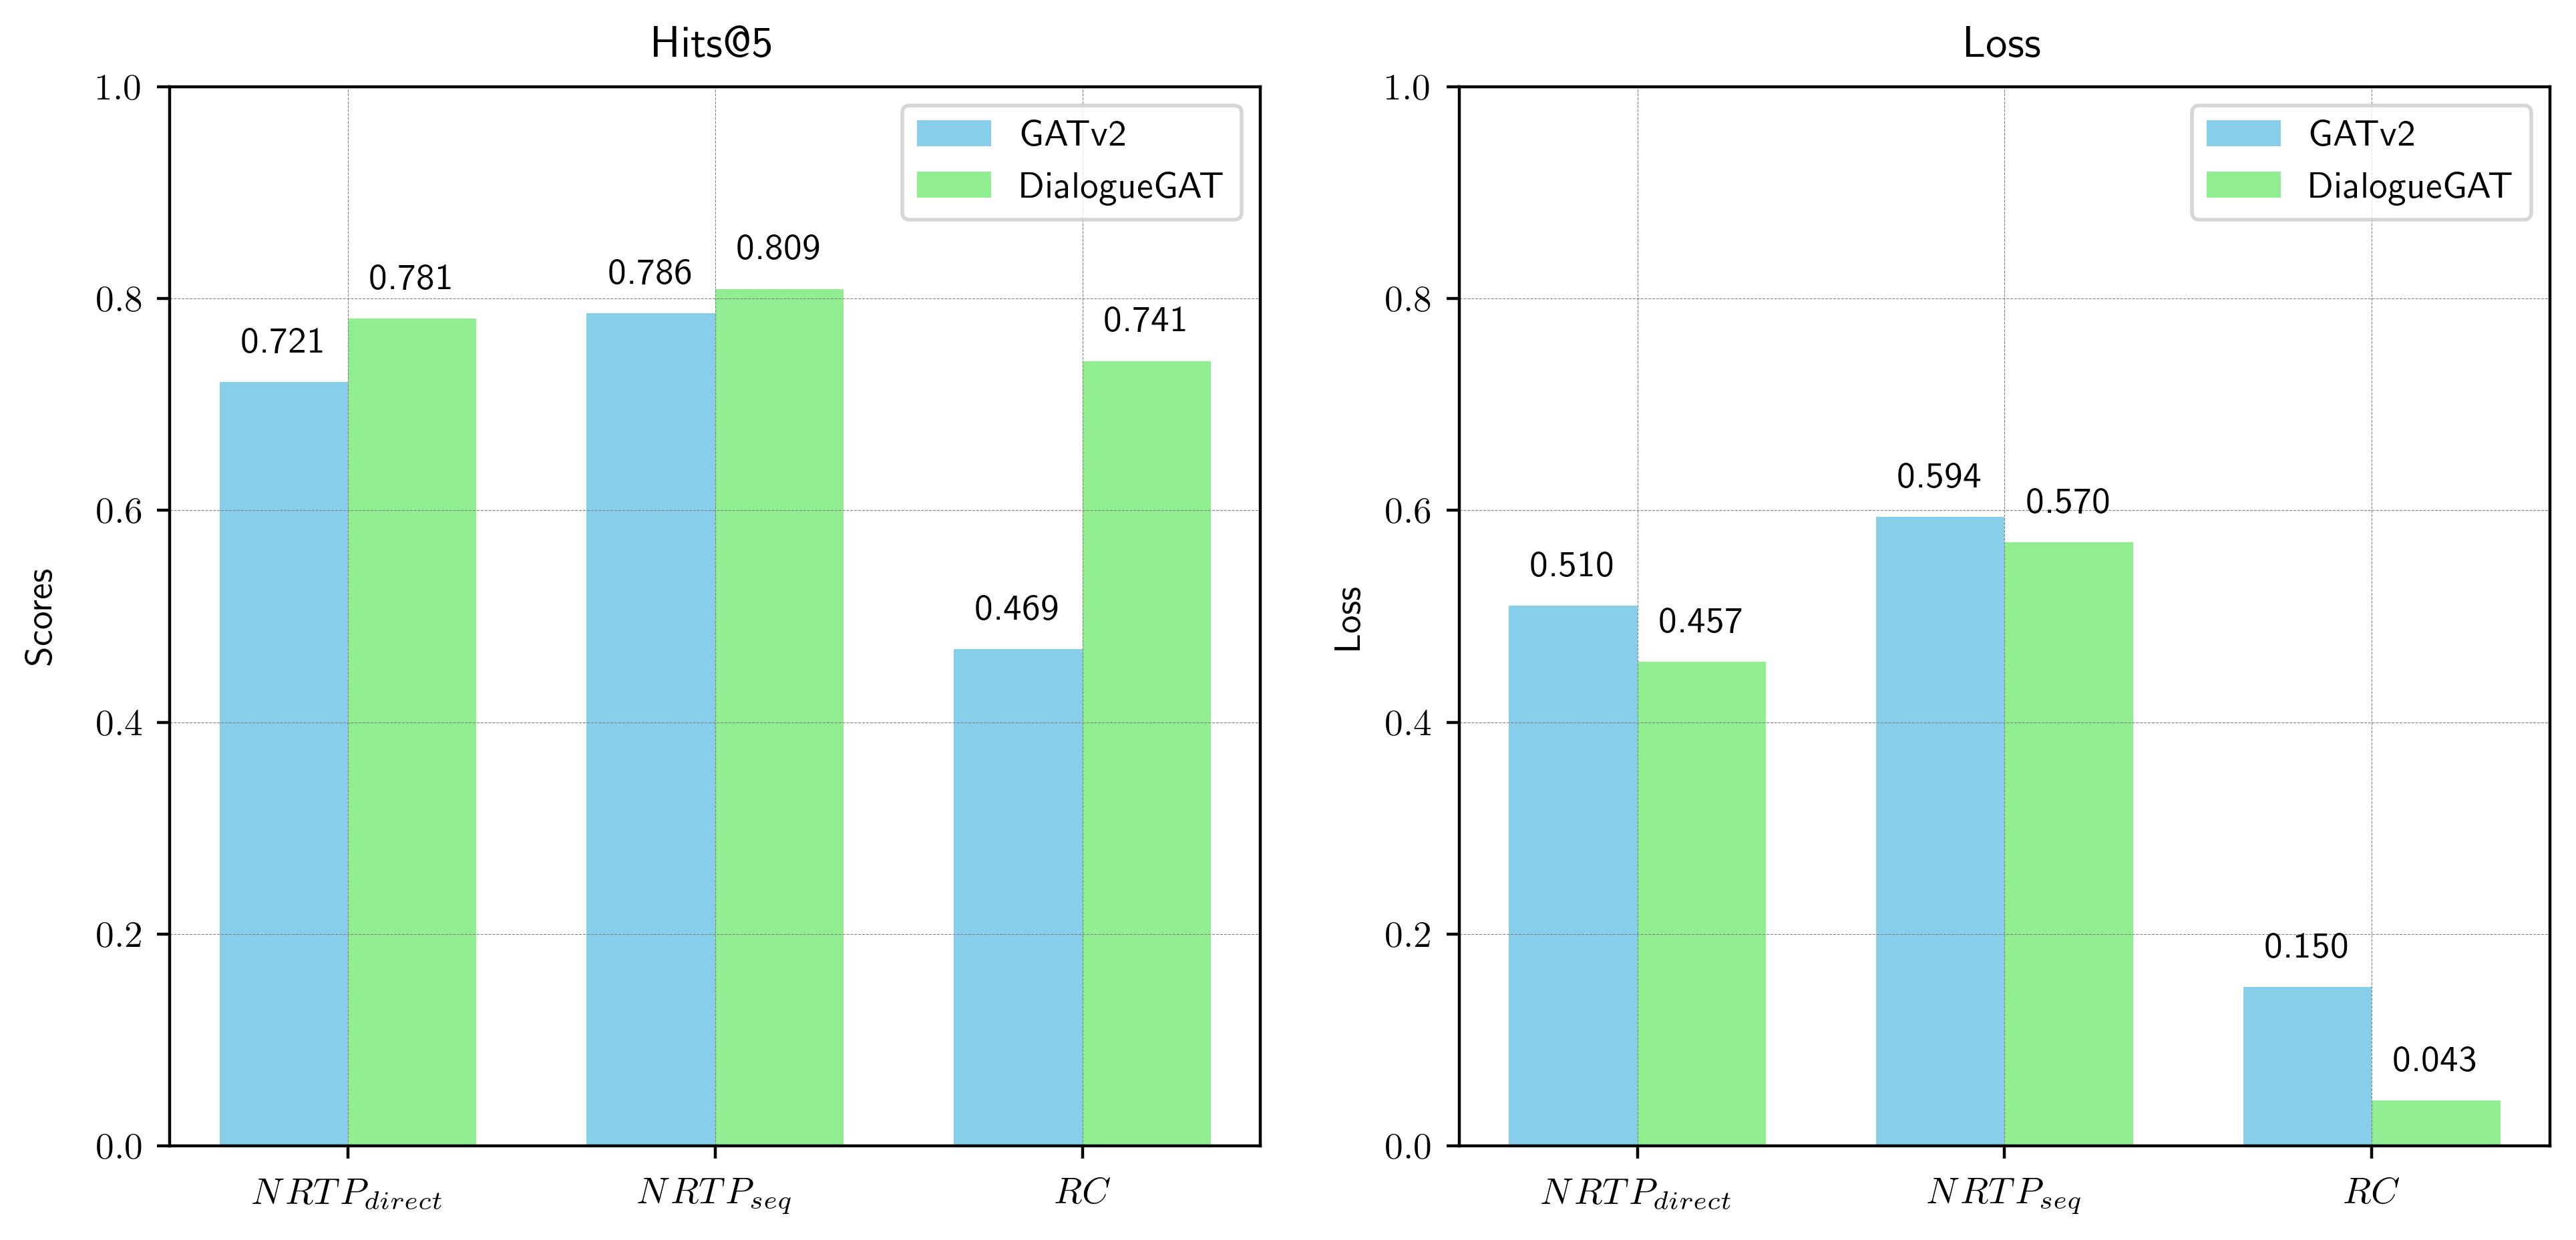
\includegraphics[width=1.0\textwidth]{./context/experiment/images/compare_gatv2_dialoguegat.png}
    \caption{Comparison of GATv2 and DialogueGAT (our proposed) as Dialogue Graph Encoders in Different Tasks. \textit{NRTP} denotes Next Response Type Prediction; \textit{RC} denotes Relations Classification.}
    \label{fig:compare_gatv2_dialoguegat}
\end{figure}

\subsection{The Effect of Dialogue Graph Encoder}
We analyze the effectiveness of the Dialogue Graph Encoder (discussed in Section 3.2.2 fine-tuning phase) under various settings. (1) \textbf{Context+Persona (Attention)}: This is our primary method where we utilize an Attention-based Feature Fusion approach to integrate representations from both the Dialogue Graph and the Persona Graph. (2) \textbf{Context+Persona (Add)}: We replace the Attention-based Feature Fusion approach with a simple addition of the persona and context representations. (3) \textbf{Context}: In this setting, we solely rely on the representation from the Dialogue Graph. (4) \textbf{Persona}: Here, we use only the representation from the Persona Graph. (5) \textbf{Random}: A random vector replaces the output of the Dialogue Graph Encoder. (6) \textbf{None}: The Dialogue Graph Encoder is completely removed from the process, allowing the generator to receive only the context and persona information from the Text Encoder. The comprehensive experimental results can be found in Figure \ref{fig:effectiveness_of_dialogue_graph_encoder}. We report the metrics for BLEU-1, ROUGE-1, and Consistency Score (C.Score).

Our experimental results demonstrate that the attention-based feature fusion approach (Context+Persona (Attention)) significantly outperforms other methods in terms of BLEU-1 and ROUGE-1 scores. These findings confirm that effectively integrating contextual and persona information through an attention mechanism enhances the similarity of the generated responses to the ground-truth responses. In contrast, simpler methods such as addition (Context+Persona (Add)) or those relying solely on context or persona information exhibit lower performance. The scores drastically decrease when random vectors are employed or when the dialogue graph encoder is omitted entirely, which emphasizes the crucial role of structured and meaningful input in producing coherent responses. The consistency scores further elucidate the models' ability to generate responses that align with persona traits. The superior performance of the attention-based method suggests its effectiveness in maintaining persona consistency within the responses. Notably, employing random vectors results in negative C.Score values, indicating that some generated responses are not only irrelevant but also contradictory to the defined personas.

These outcomes reinforce the importance of utilizing attention-based feature fusion in dialogue systems, especially in tasks that require a nuanced understanding of both context and persona. Additionally, the inferior results associated with random inputs and the complete removal of the dialogue graph encoder highlight potential risks of response incoherence and contradiction when inputs are not integrated thoughtfully. We present examples of generated results for these settings in Table \ref{table:case_study_effectiveness_of_dialogue_graph_encoder}.

\begin{figure}[H]
    \centering
    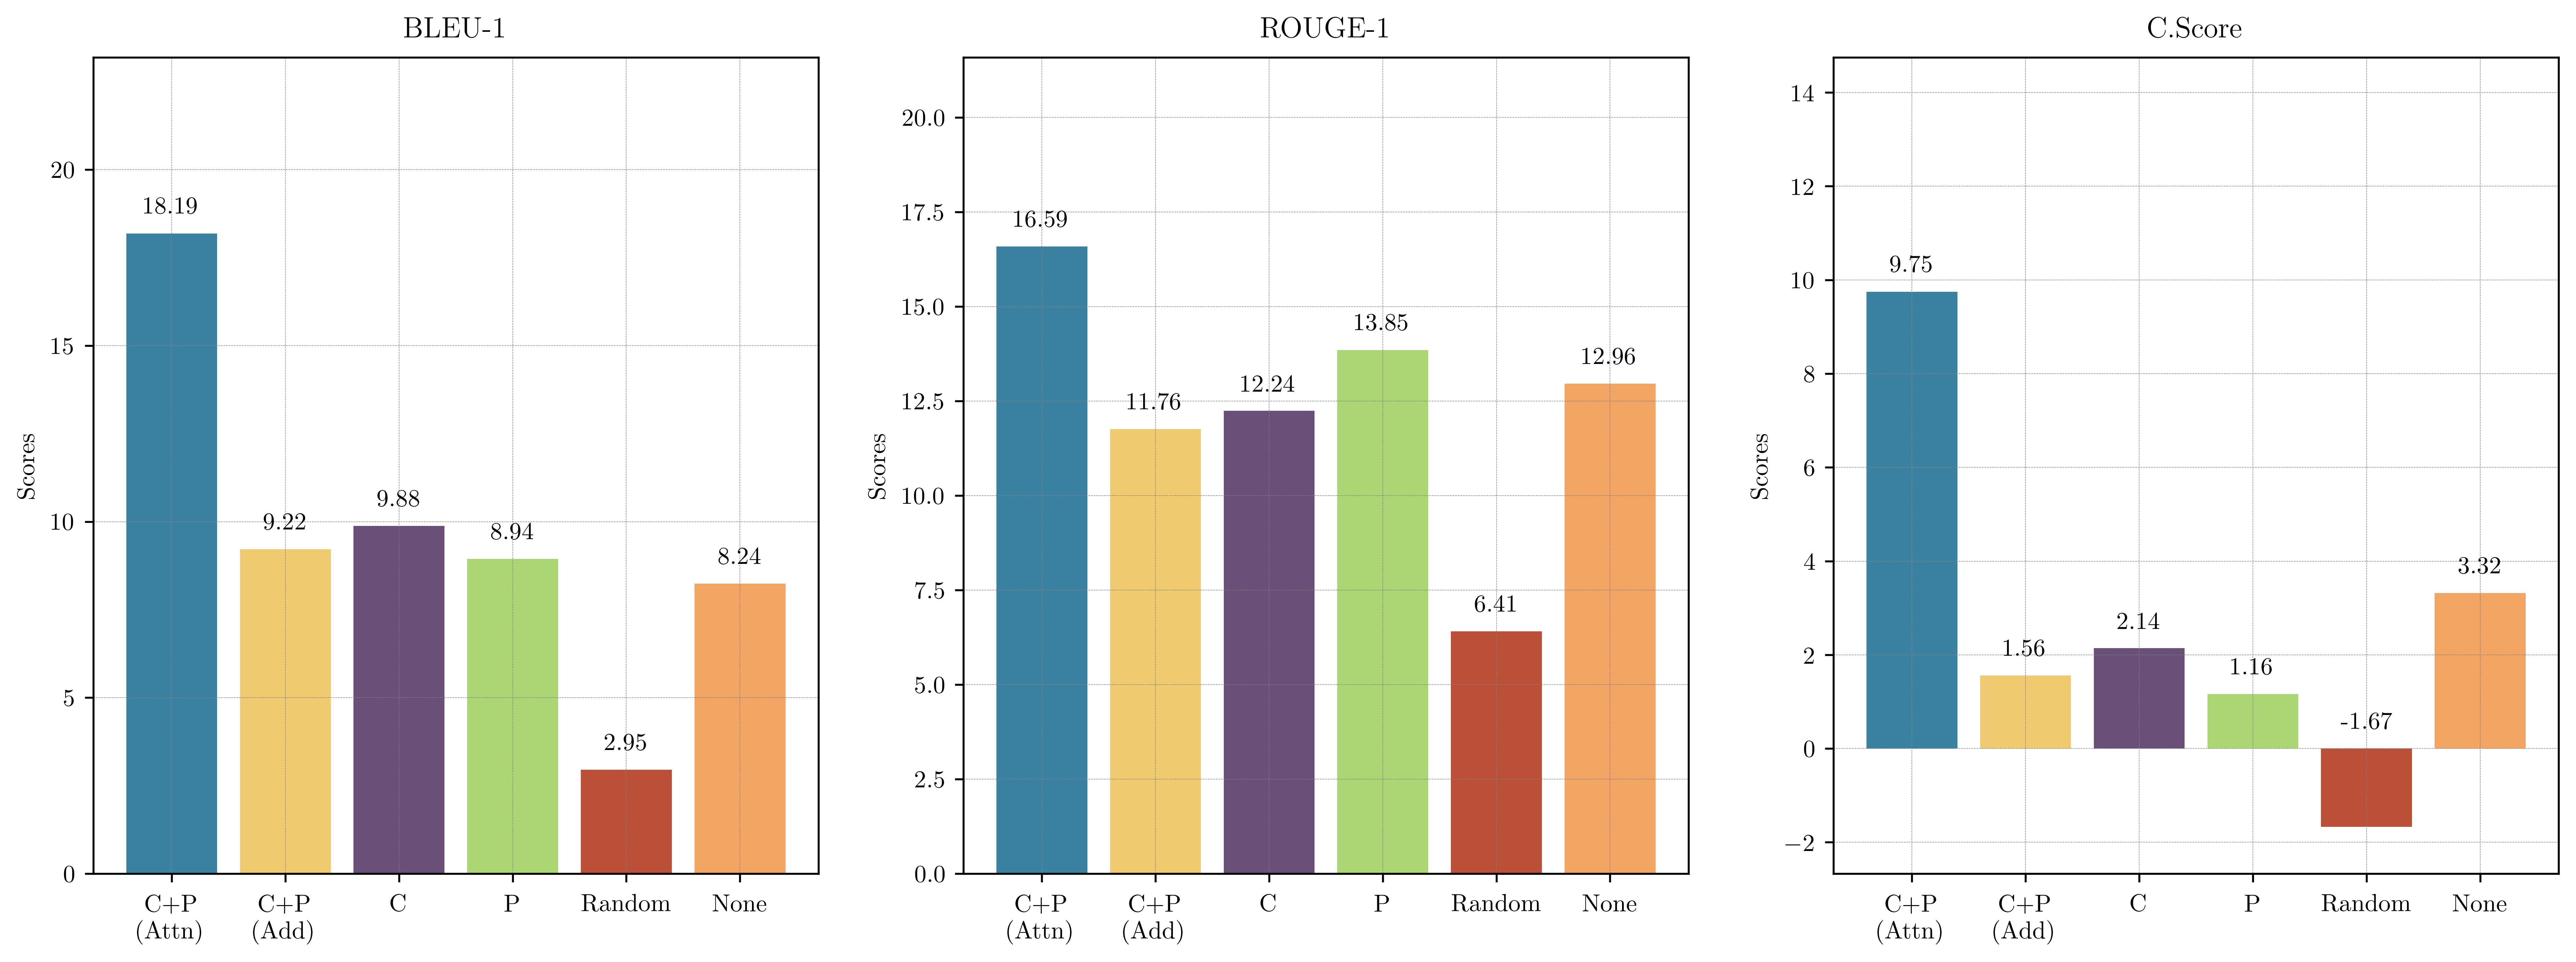
\includegraphics[width=1.0\textwidth]{./context/experiment/images/effectiveness_of_dialogue_graph_encoder.png}
    \caption{Performance analysis of Dialogue Graph Encoder across different settings. Here, "C" represents Context, and "P" represents Persona.}
    \label{fig:effectiveness_of_dialogue_graph_encoder}
\end{figure}

\subsection{The Effect of Tau Values in Dynamic Weighted Aggregation}
We analyze the effectiveness of $\tau$ in Dynamic Weighted Aggregation (discussed in Section 3.4). According to our results, shown in Figure \ref{fig:effectiveness_of_tau}, each score gradually decreases as $\tau$ increases, with the most significant drop occurring at 0.8. The metrics most noticeably affected are DEAM and C.Score, which assess coherence and personalization, respectively. Additionally, we observed that the scores, particularly for BLEU-1, actually increase when $\tau$ reaches 1.0. We hypothesize that this is due to our approach, which involves a residual connection (Eq. \ref{eq:dynamic_weighted_aggregation_output}) between the outputs of the Text Encoder and the Dialogue Graph Encoder with the results of the dynamic weighting. When $\tau$ is set to 1.0, it effectively considers only the original outputs, thus retaining a certain level of generative capability. However, this does not enhance persona-consistency and coherence as much as when $\tau$ is optimally adjusted. 

In summary, by employing Dynamic Weighted Aggregation and selecting an appropriate 
$\tau$ value, we can effectively balance coherence and personalization information, thereby generating more natural responses. This method ensures that the model not only adheres to the user-specific attributes but also maintains a logical and coherent dialogue flow, crucial for enhancing user engagement and satisfaction in interactive systems.

\begin{figure}[H]
    \centering
    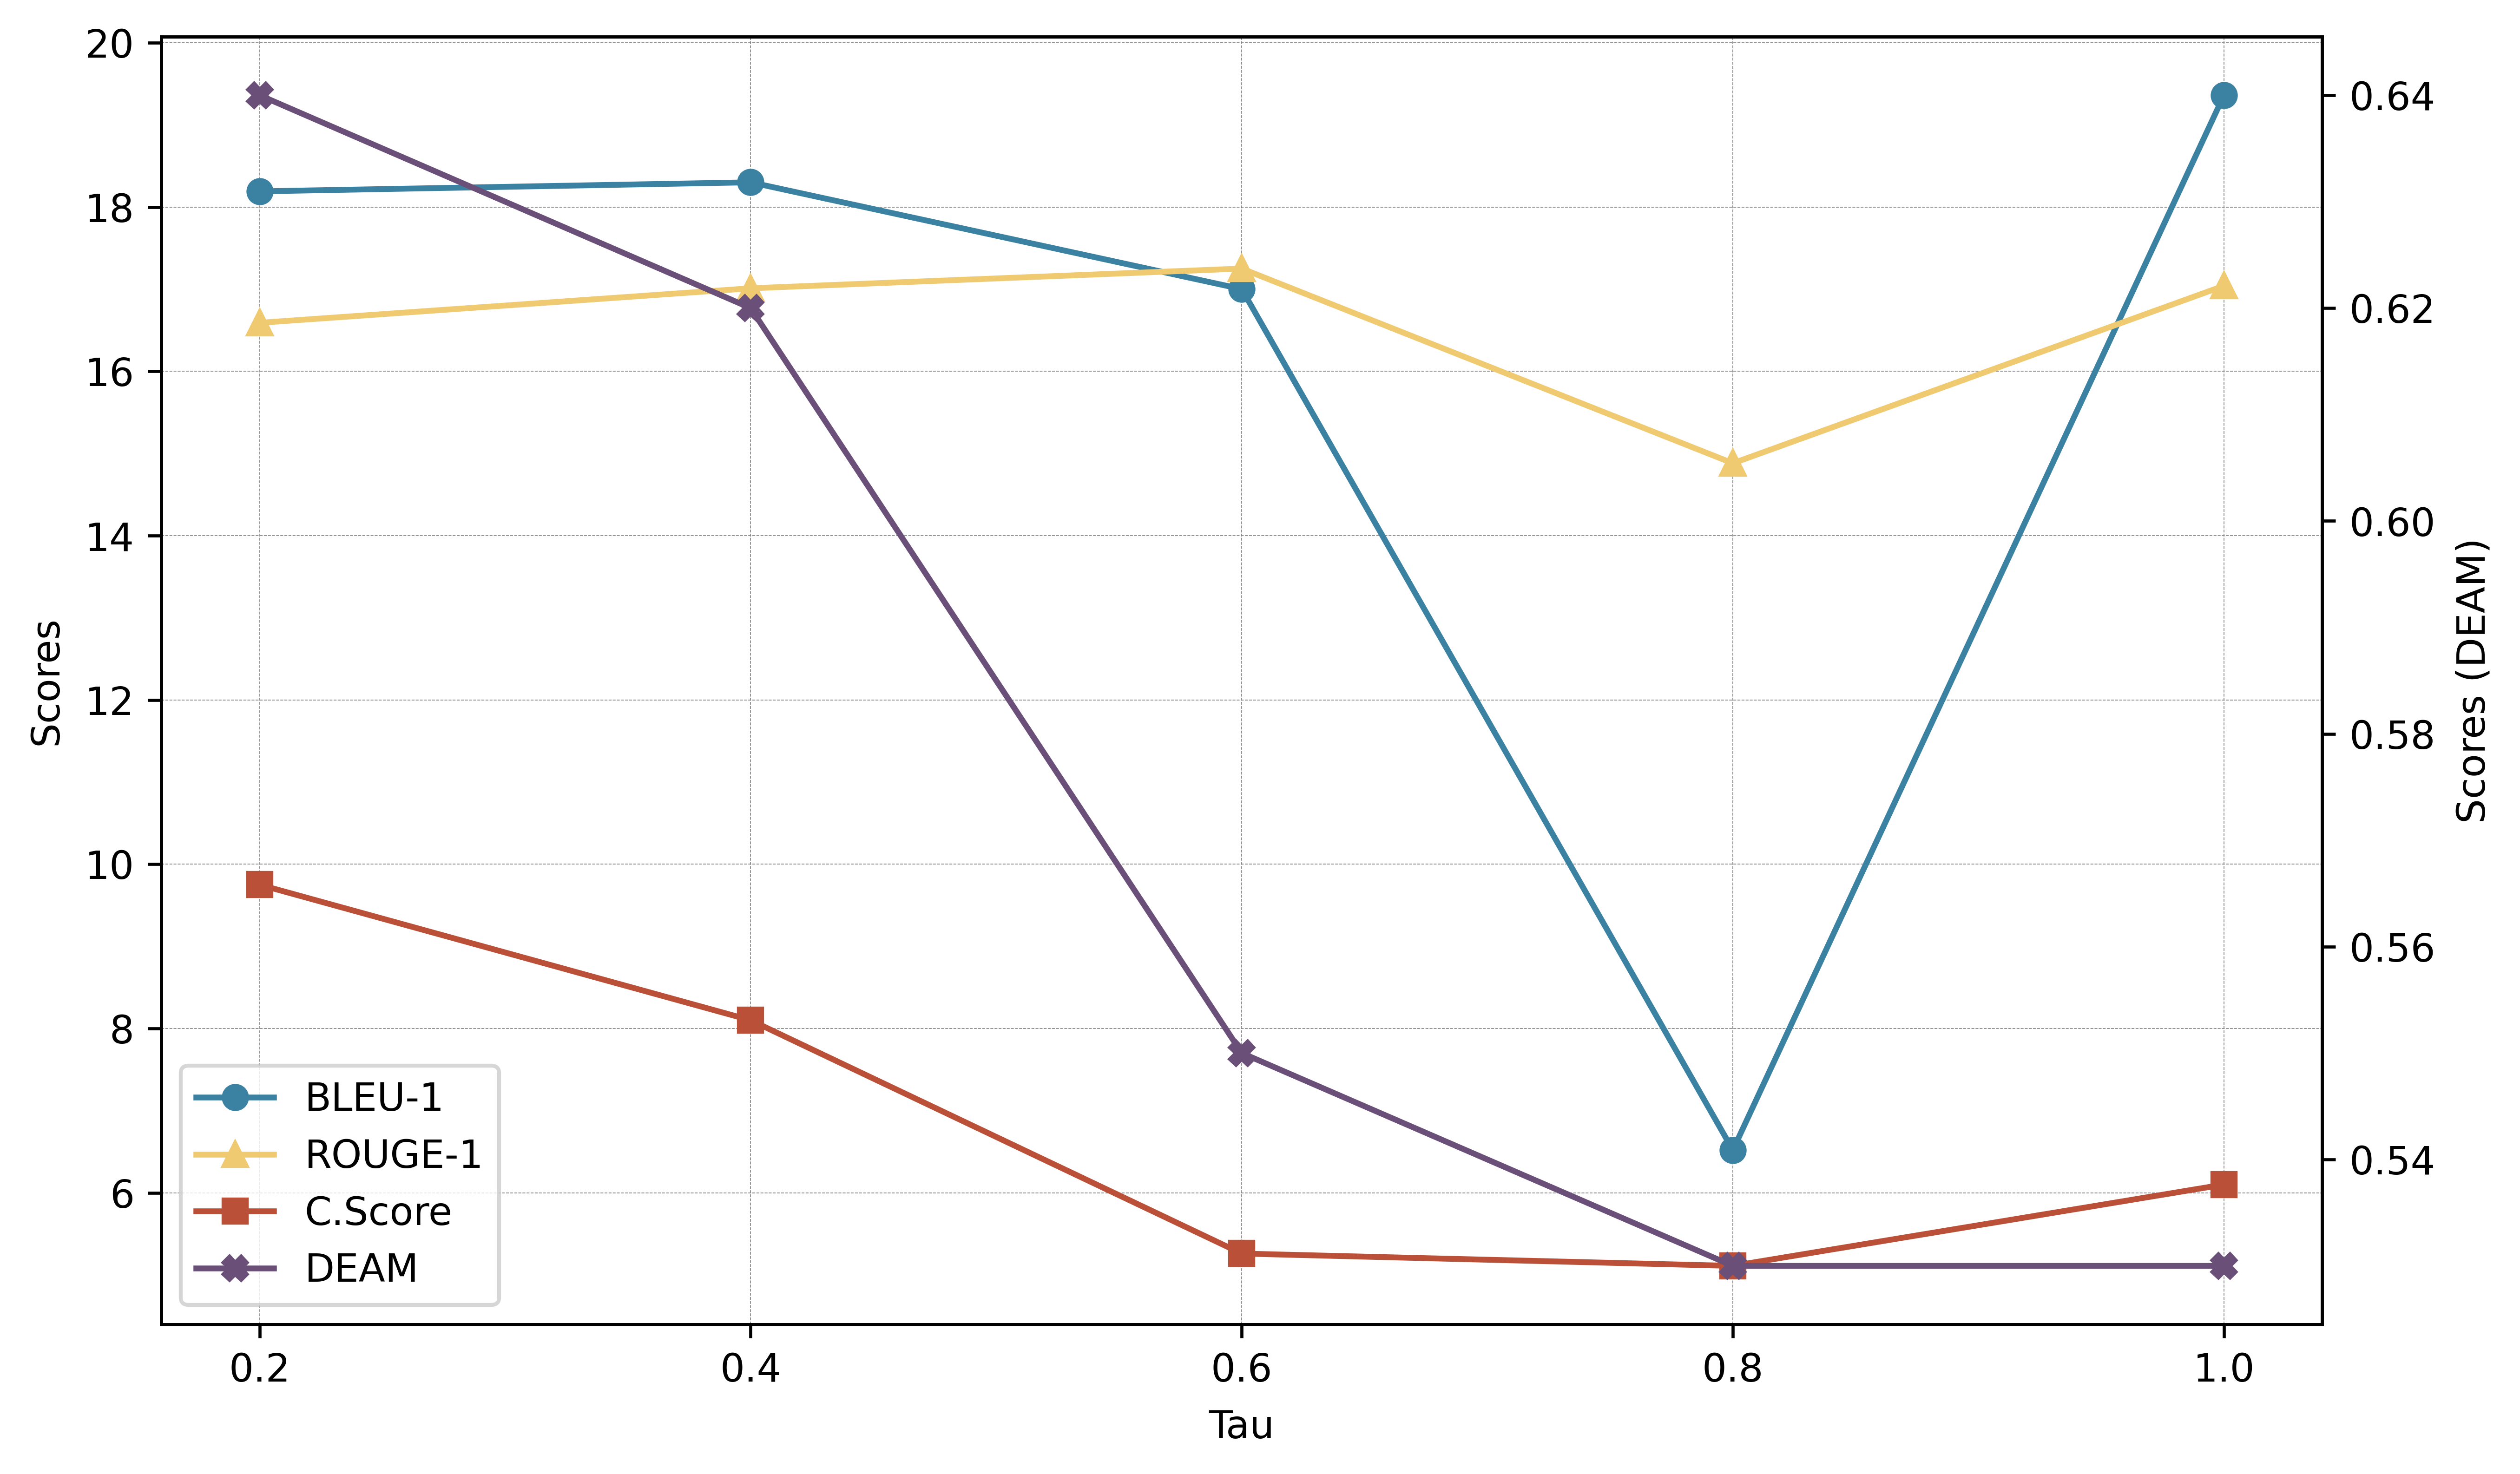
\includegraphics[width=0.9\textwidth]{./context/experiment/images/effectiveness_of_tau.png}
    \caption{Performance analysis of $\tau$ in Dynamic Weighted Aggregation.}
    \label{fig:effectiveness_of_tau}
\end{figure}

\subsection{Ablation Study}
% In our approach, to enable the dialogue graph encoder to understand the dialogue structure and adapt to subsequent coherence-related fine-tuning tasks, we designed several pre-training tasks aimed at capturing the dialogue structure. Therefore, we conducted an ablation study on these tasks to examine their impact on generating personalized responses later on. We present the results for three important metrics, coherence, personalization, and diversity, to demonstrate the impact of the pre-training task on the generated outcomes. The results of the ablation study for pre-training tasks are displayed in Table \ref{table:ablation_study}, we observed that first, after removing the Shortest Path Prediction task, the scores for coherence (QuantiDCE), persona-consistency (C.Score), and diversity (Dist-1) began to drop sharply. The goal of the Turn Classification task is to help the model capture the local structure. When this task was removed, there was a dramatic decline in scores for local coherence and persona-consistency, proving that this task aids the model in effectively capturing semantic similarities in dialogue data. Furthermore, if the Graph Reconstruction task is removed, there is a continuing downward trend in personalization scores. This confirms that our three self-supervised pretraining tasks are beneficial for the model’s understanding of dialogue structure and assist in coherence-related fine-tuning tasks, ultimately impacting the model's ability to balance coherence and persona information when generating personalized responses.

% Additionally, we conducted ablation experiments for different fine-tuning tasks. According to the conclusions drawn from Table \ref{table:ablation_study}, the removal of specific fine-tuning tasks significantly affects the model's performance metrics. Notably, the absence of tasks such as Coherence Relations Classification and Next Response Type Prediction leads to incomplete data in the table, indicating these tasks' critical roles in enhancing model accuracy and output quality. Furthermore, the removal of the Link Prediction task results in noticeable drops in both local coherence and persona consistency scores, underscoring its importance in maintaining the structural integrity and relevance of generated dialogues. These findings highlight the substantial impact that fine-tuning adjustments have on the effectiveness of the model in personalized dialogue generation.

% In our study, we investigated the impact of specific pre-training and fine-tuning tasks on the performance of a dialogue graph encoder, designed to grasp the structure of dialogues and adapt to coherence-related fine-tuning tasks. Our ablation study, summarized in Table \ref{table:ablation_study}, revealed significant declines in key performance metrics—coherence (QuantiDCE), persona-consistency (C.Score), and diversity (Dist-1)—upon the removal of these tasks. The removal of the Shortest Path Prediction (SPP) task led to sharp decreases across all metrics, underscoring its role in enhancing the encoder's capability to maintain dialogue coherence and persona consistency. Similarly, eliminating the Turn Classification (TC) task resulted in a substantial drop in local coherence and persona-consistency scores, indicating its effectiveness in capturing semantic similarities within dialogue data. Additionally, when the Graph Reconstruction (GR) task was excluded, we observed a continued decline in personalization scores, suggesting its importance in retaining a nuanced understanding of dialogue structures. Our findings were further corroborated during the fine-tuning phase, where the absence of specific tasks like Coherence Relations Classification (RC), Next Response Type Prediction (NRTP), and Link Prediction (LP) also significantly impacted model performance, particularly affecting its ability to balance coherence and personalization in generating responses. These results collectively demonstrate that both pre-training and fine-tuning tasks are crucial for optimizing the dialogue graph encoder's performance in personalized dialogue generation.

In our approach, we propose the Dialogue Graph Encoder that utilizes a two-stage training method of pretrain-finetune to allow the model to first learn dialogue structure and then further capture latent coherence relationships in dialogue data during the fine-tuning phase. To examine the impact of these diverse tasks on generating personalized responses, we conducted ablation experiments to evaluate the specific effects of removing certain pretraining and fine-tuning tasks on model performance. Experimental results summarized in Table \ref{table:ablation_study} show that when removing pre-training tasks such as Shortest Path Prediction (SPP), Turn Classification (TC), or Graph Reconstruction (GR), the model significantly decreases in key indicators like semantic consistency, persona-consistency, and diversity. Particularly, the objective of the Turn Classification (TC) task is to enable the model to predict the sequential relationship between two utterances in a dialogue, thereby learning effective utterance node representations. This aids the model's transferability to subsequent fine-tuning tasks. Hence, the removal of this task results in the largest decline in performance scores, as the model loses its capability to effectively identify local dialogue structures. These results confirm the crucial role of these pretraining tasks in helping models understand and adapt to dialogue structures, and also establish a solid foundation for subsequent supervised fine-tuning. Furthermore, ablation studies during the fine-tuning phase further emphasize the importance of tasks such as Coherence Relations Classification (RC), Next Response Type Prediction (NRTP), and Link Prediction (LP) in enhancing model performance for personalized dialogue generation. Particularly, the removal of the Coherence Relations Classification (RC) task resulted in a dramatic decrease in the model's performance in personalization assessments. This demonstrates that supervised edge-level relationship prediction tasks can aid the model in capturing potential discourse relations between adjacent nodes, learning node representations that encapsulate this information, and during subsequent Attention-based Feature Fusion, more effectively integrating utterance and persona node information for enhanced coherence and persona-consistency.

\begin{table}[ht]
    \centering
    \def\arraystretch{1.4}%
    \begin{tabular}{cccc}
    \hline
           Models & QuantiDCE & C.Score & Dist-1 \\
          \hline
          \begin{tabular}{@{}c@{}}$\textbf{MUDI}_{\text{SP}}$ \\ (ours)\end{tabular}  & 3.05 & 11.87 & 46.76 \\
          \hhline{====}
        \multicolumn{4}{c}{\textbf{Pre-training}} \\
        \hhline{====}
          \hspace*{0.65cm} w/o SPP & 2.72  & 7.05 & 34.07  \\
         \hspace*{0.5cm} w/o TC  & 2.69  & 1.18 & 33.07 \\
         \hspace*{0.5cm} w/o GR & 2.72  & 6.49 & 33.94 \\
        \hhline{====}
        \multicolumn{4}{c}{\textbf{Fine-tuning}} \\
        \hhline{====}
        \hspace*{0.5cm} w/o RC & 2.77  & 0.54 & 31.91  \\
         \hspace*{1.0cm} w/o NRTP  & 2.95  & 2.83 & 31.15 \\
         \hspace*{0.5cm} w/o LP & 2.69  & 6.22 & 34.04 \\
    \hline
    \end{tabular}
    \caption{Ablation study of the Dialogue Graph Encoder for pre-training and fine-tuning tasks.}
    \label{table:ablation_study}
\end{table}


\begin{table}[H]
\centering
\def\arraystretch{1.0}%
\begin{tabular}{|p{3.5cm}|p{12cm}|}

\hline
\rowcolor{yellow}
\multicolumn{2}{|c|}{\textbf{Persona}} \\
\hline
\multicolumn{2}{|l|}{I have two dogs.} \\
\multicolumn{2}{|l|}{I like to work on vintage cars.} \\
\multicolumn{2}{|l|}{My favorite music is country.} \\
\multicolumn{2}{|l|}{I own two vintage mustangs.} \\
\hline

\rowcolor{yellow}
\multicolumn{2}{|c|}{\textbf{Context}} \\
\hline
\multicolumn{2}{|l|}{Q: Hi! How are you doing tonight?} \\
\multicolumn{2}{|l|}{R: I'm doing great. Just relaxing with my two dogs.} \\
\multicolumn{2}{|l|}{Q: Great. In my spare time I do volunteer work.} \\
\multicolumn{2}{|l|}{R: That's neat. What kind of volunteer work do you do?} \\
\multicolumn{2}{|l|}{Q: I work in a homeless shelter in my town.} \\
\multicolumn{2}{|l|}{R: Good for you. Do you like vintage cars? I've two older mustangs.} \\
\multicolumn{2}{|l|}{Q: Cool. Not really into cars. My day job is wrestling.} \\
\multicolumn{2}{|l|}{R: Cars are my thing. Vintage cars. I love working on them. Wrestling? Do you enjoy it?} \\
\multicolumn{2}{|l|}{Q: Yes, I love the crowds, getting to know people.} \\
\multicolumn{2}{|l|}{R: I didn't think about the crowd aspect of wrestling. I do not like crowds.} \\
\multicolumn{2}{|l|}{Q: Understood. When I need to be alone, I work out a few times each week.} \\
\multicolumn{2}{|l|}{R: I agree. Working out is a great way to burn off steam. Do you like country music?} \\
\hline

\rowcolor{yellow}
\multicolumn{2}{|c|}{\textbf{Query}} \\
\hline
\multicolumn{2}{|l|}{A little bit. I can get into taylor swift.} \\

\hhline{|==|}
\rowcolor[RGB]{204,217,245}
\multicolumn{2}{|c|}{\textbf{Response}} \\
\hhline{|==|}
\textbf{Context+Persona (Attention)} & I do not like her. She's a bit too uptight for my taste. But I like her music. \\
\textbf{Context+Persona (Add)} & I can get may may and m and may and j on for more of her \\
\textbf{Context} &  What was she like? \\
\textbf{Persona} & I like country music too. \\
\textbf{Random} & you The A’ A A played The old White lead A Barbara at The The 17… \\
\textbf{None} & I like country music as well. \\

\hline
\end{tabular}
\caption{Case analysis of the effectiveness of Dialogue Graph Encoder.}
\label{table:case_study_effectiveness_of_dialogue_graph_encoder}
\end{table}

\subsection{Case Study}
Teable \ref{table:case_study_1}, \ref{table:case_study_2}, \ref{table:case_study_3}, and \ref{table:case_study_4} present the personalized responses generated by various methods using the ConvAI2 dataset. The responses generated by the proposed method, \textbf{MUDI}, demonstrated greater consistency with their respective personas and showed higher coherence with both the context and the query, appearing more human-like. As illustrated in Table \ref{table:case_study_1}, the responses from BoB were incoherent with the query, though they remained consistent with the persona. PAA often overfocused on the persona, leading to repetitive narratives of the persona description. Both LMEDR and our model produced responses that were more coherent, basing them on the user persona, but MUDI was able to generate more detailed replies, such as adding personal aspirations to the basic response about family support. 

In Table \ref{table:case_study_2}, the responses generated by BoB were irrelevant to the personas and incoherent with the context. PAA exhibited a global incoherence from the dialogue context, failing to maintain a logical flow in the conversation. While LMEDR generated a somewhat relevant response indicating a dream car, it lacked depth and personal context. On the other hand, MUDI produced a more personalized and contextually rich response that not only mentions the dream car but also integrates family dynamics, demonstrating a deeper understanding of the persona's background and the complexities in their personal relationships. 

In Table \ref{table:case_study_3}, BoB and PAA tended to overlook content from the ongoing dialogue, generating repetitive responses that rendered the entire conversation incoherent. Although LMEDR was able to generate adequate responses, our model excelled by producing more natural responses through the inclusion of responsive questions. 

As shown in Table \ref{table:case_study_4}, BoB diverged from the persona's preference by mentioning classic rock instead of country music, showing a misalignment with the user’s interests. LMEDR and PAA both correctly identified and responded with a generic appreciation for country music, aligning with the persona’s interests, yet their responses lacked specific engagement with the user’s mention of Taylor Swift or deeper personal nuances. MUDI's response, while initially not favoring Taylor Swift, cleverly circled back to acknowledge her music, demonstrating not only a nuanced understanding of the persona's tastes but also adding an interesting twist to the conversation. This illustrates MUDI's ability to generate engaging and lifelike responses, making the interaction more intriguing for users.

In summary, our model \textbf{MUDI} effectively combines dialogue and persona elements to generate appropriate responses. Furthermore, it excels at using responsive questions to enhance the conversation's naturalness.


% ----------------------------------------------
% Case Study 1
% ----------------------------------------------

\begin{table}[ht]
\centering
\def\arraystretch{1.6}%
\begin{tabular}{|l|p{11cm}|}

\hline
\rowcolor{yellow}
\multicolumn{2}{|c|}{\textbf{Persona}} \\
\hline
\multicolumn{2}{|l|}{My dream car is a rolls royce ghost.} \\
\multicolumn{2}{|l|}{I currently work for a watch dealer.} \\
\multicolumn{2}{|l|}{My family does not support my career choices.} \\
\multicolumn{2}{|l|}{I often shop for shoes and watches.} \\
\multicolumn{2}{|l|}{I like shopping.} \\
\hline

\rowcolor{yellow}
\multicolumn{2}{|c|}{\textbf{Context}} \\
\hline
\multicolumn{2}{|l|}{Q: Good evening. What are you up to?} \\
\multicolumn{2}{|l|}{R: Hello, how are you ? I am well. I like to shop for shoes and watches.} \\
\multicolumn{2}{|l|}{Q: I don't shop much. Prefer to relax at home with my cow.} \\
\multicolumn{2}{|l|}{R: What do you do ? I'm work for a watch dealer.} \\
\hline

\rowcolor{yellow}
\multicolumn{2}{|c|}{\textbf{Query}} \\
\hline
\multicolumn{2}{|l|}{No wonder you like watches ! I'm a commercial electrician.} \\

\hhline{|==|}
\rowcolor[RGB]{204,217,245}
\multicolumn{2}{|c|}{\textbf{Response}} \\
\hhline{|==|}
\textbf{GOLD} & wonderful! yeah, however, my family does not support my choice of career. \\
\textbf{BoB} & I work at a dealership, but I am not very good at it. \\
% \textbf{P$^2$BOT} & what do you do for a living ? i work for the watch. \\
\textbf{LMEDR} & My family does not support my career choices. \\
\textbf{PAA} & I like to shop. I also like to shop. \\
\textbf{MUDI} & My family does not support my career choices. I want to drive a rolls royce ghost. \\

\hline
\end{tabular}
\caption{Case analysis of personalized response generation on the ConvAI2 dataset.}
\label{table:case_study_1}
\end{table}

% ----------------------------------------------
% Case Study 2
% ----------------------------------------------

\begin{table}[ht]
\centering
\def\arraystretch{1.6}%
\begin{tabular}{|l|p{11cm}|}

\hline
\rowcolor{yellow}
\multicolumn{2}{|c|}{\textbf{Persona}} \\
\hline
\multicolumn{2}{|l|}{My dream car is a rolls royce ghost.} \\
\multicolumn{2}{|l|}{I currently work for a watch dealer.} \\
\multicolumn{2}{|l|}{My family does not support my career choices.} \\
\multicolumn{2}{|l|}{I often shop for shoes and watches.} \\
\multicolumn{2}{|l|}{I like shopping.} \\
\hline

\rowcolor{yellow}
\multicolumn{2}{|c|}{\textbf{Context}} \\
\hline
\multicolumn{2}{|l|}{Q: Good evening. What are you up to?} \\
\multicolumn{2}{|l|}{R: Hello, how are you ? I am well. I like to shop for shoes and watches.} \\
\multicolumn{2}{|l|}{Q: I don't shop much. Prefer to relax at home with my cow.} \\
\multicolumn{2}{|l|}{R: What do you do ? I'm work for a watch dealer.} \\
\multicolumn{2}{|l|}{Q: No wonder you like watches! I'm a commercial electrician.} \\
\multicolumn{2}{|l|}{R: Wonderful! Yeah, however, my family does not support my choice of career.} \\
\hline

\rowcolor{yellow}
\multicolumn{2}{|c|}{\textbf{Query}} \\
\hline
\multicolumn{2}{|l|}{Why not? Family is important.} \\

\hhline{|==|}
\rowcolor[RGB]{204,217,245}
\multicolumn{2}{|c|}{\textbf{Response}} \\
\hhline{|==|}
\textbf{GOLD} & I'm not sure why they do not. Do you like cars? \\
\textbf{BoB} & I am not sure. I am a watch dealer. \\
% \textbf{P$^2$BOT} & my family doesn't support my lifestyle choices. \\
\textbf{LMEDR} & I do not know. I do have a dream car though. It is a rolls royce ghost. \\
\textbf{PAA} & I am a watch dealer. I have a lot of money. \\
\textbf{MUDI} & yes agree! I want to drive a rolls royce ghost car, but my family does not like that. \\

\hline
\end{tabular}
\caption{Case analysis of personalized response generation on the ConvAI2 dataset.}
\label{table:case_study_2}
\end{table}

% ----------------------------------------------
% Case Study 3
% ----------------------------------------------

\begin{table}[ht]
\centering
\def\arraystretch{1.6}%
\begin{tabular}{|l|p{11cm}|}

\hline
\rowcolor{yellow}
\multicolumn{2}{|c|}{\textbf{Persona}} \\
\hline
\multicolumn{2}{|l|}{I listen to rap music.} \\
\multicolumn{2}{|l|}{I produce music for artists.} \\
\multicolumn{2}{|l|}{I drive a 2015 Honda Civic.} \\
\multicolumn{2}{|l|}{My favorite food is pizza.} \\
\hline

\rowcolor{yellow}
\multicolumn{2}{|c|}{\textbf{Context}} \\
\hline
\multicolumn{2}{|l|}{Q: Hi, how are you? Do you have any brothers or sisters?} \\
\multicolumn{2}{|l|}{R: No I don't do you?} \\
\multicolumn{2}{|l|}{Q: Yes, I'm 13 and I've an older brother.} \\
\multicolumn{2}{|l|}{R: That's nice what kind of music do you like.} \\
\multicolumn{2}{|l|}{Q: I do not have much time as I play soccer. You?} \\
\multicolumn{2}{|l|}{R: I am a music producer for rap artists} \\
\hline

\rowcolor{yellow}
\multicolumn{2}{|c|}{\textbf{Query}} \\
\hline
\multicolumn{2}{|l|}{Cool I like rap. I hate maths though! Do you have other hobbies?} \\

\hhline{|==|}
\rowcolor[RGB]{204,217,245}
\multicolumn{2}{|c|}{\textbf{Response}} \\
\hhline{|==|}
\textbf{GOLD} & Work takes up a lot of my time. \\
\textbf{BoB} & I like music and I like to listen to music. \\
% \textbf{P$^2$BOT} & I like to listen to rap music. \\
\textbf{LMEDR} & I like to drive my honda civic. \\
\textbf{PAA} & I like rap music, I produce it for artists. \\
\textbf{MUDI} & I like to go my old Honda Civic car and eat pizza. Do you have any hobbies? \\

\hline
\end{tabular}
\caption{Case analysis of personalized response generation on the ConvAI2 dataset.}
\label{table:case_study_3}
\end{table}

% ----------------------------------------------
% Case Study 4
% ----------------------------------------------

\begin{table}[ht]
\centering
\def\arraystretch{1.6}%
\begin{tabular}{|l|p{11cm}|}

\hline
\rowcolor{yellow}
\multicolumn{2}{|c|}{\textbf{Persona}} \\
\hline
\multicolumn{2}{|l|}{I have two dogs.} \\
\multicolumn{2}{|l|}{I like to work on vintage cars.} \\
\multicolumn{2}{|l|}{My favorite music is country.} \\
\multicolumn{2}{|l|}{I own two vintage mustangs.} \\
\hline

\rowcolor{yellow}
\multicolumn{2}{|c|}{\textbf{Context}} \\
\hline
\multicolumn{2}{|l|}{Q: Hi! How are you doing tonight?} \\
\multicolumn{2}{|l|}{R: I'm doing great. Just relaxing with my two dogs.} \\
\multicolumn{2}{|l|}{Q: Great. In my spare time I do volunteer work.} \\
\multicolumn{2}{|l|}{R: That's neat. What kind of volunteer work do you do?} \\
\multicolumn{2}{|l|}{Q: I work in a homeless shelter in my town.} \\
\multicolumn{2}{|l|}{R: Good for you. Do you like vintage cars? I've two older mustangs.} \\
\multicolumn{2}{|l|}{Q: Cool. Not really into cars. My day job is wrestling.} \\
\multicolumn{2}{|l|}{R: Cars are my thing. Vintage cars. I love working on them. Wrestling? Do you enjoy it?} \\
\multicolumn{2}{|l|}{Q: Yes, I love the crowds, getting to know people.} \\
\multicolumn{2}{|l|}{R: I didn't think about the crowd aspect of wrestling. I do not like crowds.} \\
\multicolumn{2}{|l|}{Q: Understood. When I need to be alone, I work out a few times each week.} \\
\multicolumn{2}{|l|}{R: I agree. Working out is a great way to burn off steam. Do you like country music?} \\
\hline

\rowcolor{yellow}
\multicolumn{2}{|c|}{\textbf{Query}} \\
\hline
\multicolumn{2}{|l|}{A little bit. I can get into taylor swift.} \\

\hhline{|==|}
\rowcolor[RGB]{204,217,245}
\multicolumn{2}{|c|}{\textbf{Response}} \\
\hhline{|==|}
\textbf{GOLD} & lol. She's more pop now. Her old stuff was country. I like classic country. \\
\textbf{BoB} & I'm not much into music. I like classic rock. \\
% \textbf{P$^2$BOT} &  \\
\textbf{LMEDR} & Yes, I love country music. \\
\textbf{PAA} & I do. I love to listen to country music. \\
\textbf{MUDI} & I do not like her. She's a bit too uptight for my taste. But I like her music. \\

\hline
\end{tabular}
\caption{Case analysis of personalized response generation on the ConvAI2 dataset.}
\label{table:case_study_4}
\end{table}

% ------------------------------------------------
\EndChapter
% ------------------------------------------------


% Conclusion chapter
% ------------------------------------------------
\StartChapter{Conclusion}{chapter:conclusion}
% ------------------------------------------------
In this work, we propose a new method, \textbf{MUDI}, to effectively model discourse relations in personalized dialogue generation. To the best of our knowledge, \textbf{MUDI} is the first framework to jointly integrate Discourse Relations and Persona in Personalized Dialogue. Firstly, we propose DialogueGAT, a dialogue-enhanced GNN, as a Dialogue Graph Encoder, designed to capture dialogue structure and contextual discourse relations. Additionally, we utilize an Attention-Based Feature Fusion method to effectively integrate context relations and persona information. We further enhance our model by employing a Text Encoder to capture persona-aware dialogue representations. We increase the decoder's ability to consider coherent information while predicting the next token by leveraging both a prompt-based conditional dialogue generation mechanism, which uses prompts to guide the response generation process, and our coherence-aware attention mechanism, which incorporates learnable embeddings and token representations. Finally, we leverage Dynamic Weighting Aggregation to balance the information between coherence-aware and persona-aware dialogue representations, ensuring a robust integration of both elements.

Extensive experiments and analyses demonstrate that our method, \textbf{MUDI}, significantly improves the quality of personalized responses by making them more coherent, informative, and aligned with the user's persona traits, as well as more human-like.

% ------------------------------------------------
\EndChapter
% ------------------------------------------------


% Future work chapter
%\input{./context/future-work/future-work}

% ------------------------------------------------

% 參考文獻 References
% References and bibliography

% Import the files that contain your references.
% If you set some references file,
% you need to use at least one cite to make Latex work.

\ReferencesFiles{./thesis/context/references/paper}{./thesis/context/references/misc}{./thesis/context/references/book}

% ------------------------------------------------

% 附錄 Appendix
%% ------------------------------------------------
\StartAppendix
% ------------------------------------------------

\input{./example/appendix/acceptable-dept}
\input{./example/appendix/submit-flow}
\input{./example/appendix/thesis-spec}
\input{./example/appendix/e-paper_upload}
\input{./example/appendix/e-paper_upload_ppt}
\input{./example/appendix/oral-notice}
\input{./example/appendix/faq}
\input{./example/appendix/unicode-symbols}

% ------------------------------------------------
\EndAppendix
% ------------------------------------------------


% ------------------------------------------------
}
  %
  % End of thesis
  \EndThesis
} % End of \newcommand{}

% ----------------------------------------------------------------------------

%
% This file is part of the project of
% National Cheng Kung University (NCKU) Thesis/Dissertation Template in LaTex.
% This project is hold at
%     <https://github.com/wengan-li/ncku-thesis-template-latex>
% by Wen-Gan Li.
%
% This project is distributed in the hope of usefuling to someone,
% you can redistribute it and/or modify it under the terms of the
% Attribution-NonCommercial-ShareAlike 4.0 International.
%
% You should have received a copy of the
% Attribution-NonCommercial-ShareAlike 4.0 International
% along with this project.
% If not, see <http://creativecommons.org/licenses/by-nc-sa/4.0/legalcode.txt>.
%
% Please feel free to fork it, modify it, and try it.
% Have fun !!!
%

% Some helper function about page

% ----------------------------------------------------------------------------

\newcommand{\StartNewPage}
{
  % Page start
  \newpage
  \phantomsection
} % End of \newcommand{}

\newcommand{\EndOfPage}
{
  % End of page
  \clearpage
} % End of \newcommand{}

% ----------------------------------------------------------------------------

% 圖書館要求中/英文摘要是由羅馬數字頁碼'i'開始, 而非由封面算起.

\def\ValueEnablePageNumberCounting{1}
\def\ValueDisablePageNumberCounting{0}
\def\VarPageNumberCounting{\ValueEnablePageNumberCounting}
\def\GetPageNumberCounting{\VarPageNumberCounting}
\newcommand{\SetPageNumberCounting}[1]{\renewcommand{\VarPageNumberCounting}{#1}}

\def\ResetPageNumberCounting{%
  \ifthenelse{\equal{\GetPageNumberCounting}{\ValueEnablePageNumberCounting}}%
  {%
    \setcounter{page}{1}
    \SetPageNumberCounting{\ValueDisablePageNumberCounting}%
  }%
  {}%
} % End of \def{}

% ----------------------------------------------------------------------------

%
% This file is part of the project of
% National Cheng Kung University (NCKU) Thesis/Dissertation Template in LaTex.
% This project is hold at
%     <https://github.com/wengan-li/ncku-thesis-template-latex>
% by Wen-Gan Li.
%
% This project is distributed in the hope of usefuling to someone,
% you can redistribute it and/or modify it under the terms of the
% Attribution-NonCommercial-ShareAlike 4.0 International.
%
% You should have received a copy of the
% Attribution-NonCommercial-ShareAlike 4.0 International
% along with this project.
% If not, see <http://creativecommons.org/licenses/by-nc-sa/4.0/legalcode.txt>.
%
% Please feel free to fork it, modify it, and try it.
% Have fun !!!
%

% Some helper function use in cover

% ----------------------------------------------------------------------------
\newcommand{\StartCover}
{
  %
  \singlespacing%
  %
  \StartNewPage
  %
  % 設定使用 無頁碼
  \thispagestyle{empty}
  %
  \EnableCoverPageStyle
  %
} % End of \newcommand{}

\newcommand{\EndCover}
{
  \DisableCoverPageStyle
  \EndOfPage
  \UseDefaultLineStretch
} % End of \newcommand{}
% ----------------------------------------------------------------------------

% --- University name 學校名字 ---
\newcommand\VarUniversityChiName{國立成功大學}           % Default
\newcommand\VarUniversityEngName{National Cheng Kung University} % Default

\newcommand{\SetUniversityChiName}[1]{%
  \renewcommand{\VarUniversityChiName}{#1}%
} % End of \newcommand{}

\newcommand{\SetUniversityEngName}[1]{%
  \renewcommand{\VarUniversityEngName}{#1}%
} % End of \newcommand{}

\newcommand{\SetUniversityName}[2]
{%
  \SetUniversityChiName{#1}%
  \SetUniversityEngName{#2}%
} % End of \newcommand{}

\newcommand{\GetUniversityChiName}{\VarUniversityChiName}
\newcommand{\GetUniversityEngName}{\VarUniversityEngName}
% ----------------------------------------------------------------------------

% --- Chinese / English title 中英文論文題目 ---
\newcommand{\VarThesisChiName}{Chinese Title Here} % Default
\newcommand{\VarThesisEngName}{English Title Here} % Default
\newcommand{\SetChiTitle}[1]{\renewcommand{\VarThesisChiName}{#1}}
\newcommand{\SetEngTitle}[1]{\renewcommand{\VarThesisEngName}{#1}}
\newcommand{\SetTitle}[2]
{
  \SetChiTitle{#1}
  \SetEngTitle{#2}
} % End of \newcommand{}

\newcommand{\GetChiTitle}{\VarThesisChiName}
\newcommand{\GetEngTitle}{\VarThesisEngName}

% ----------------------------------------------------------------------------

% --- User's name 使用者名字 ---
\newcommand{\VarMyChiName}{你的名字}     % Default
\newcommand{\VarMyEngName}{Your name}   % Default
\newcommand{\SetMyChiName}[1]{\renewcommand{\VarMyChiName}{#1}}
\newcommand{\SetMyEngName}[1]{\renewcommand{\VarMyEngName}{#1}}
\newcommand{\SetMyName}[2]
{
  \SetMyChiName{#1}
  \SetMyEngName{#2}
} % End of \newcommand{}

\newcommand{\GetAuthorChiName}{\VarMyChiName}
\newcommand{\GetAuthorEngName}{\VarMyEngName}

% ----------------------------------------------------------------------------

% --- Degree name 學位 ---
% thesis 是指論文的通稱
% dissertation 指的是博士的論文

% 碩士論文  Master's thesis
% 博士論文  Doctoral dissertation

\newcommand{\ValueDegreeMaster}{0}
\newcommand{\ValueDegreePhd}{1}
\newcommand{\FlagDegreeType}{\ValueDegreePhd} % Default
\newcommand{\GetFlagDegreeType}{\FlagDegreeType}
\newcommand{\SetFlagDegreeType}[1]{\renewcommand{\FlagDegreeType}{#1}}

\newcommand{\VarDegreeChiName}{碩士/博士} % Default
\newcommand{\VarDegreeEngName}{Master / Doctor} % Default
\newcommand{\degreeThesisEname}{Master's Thesis / Doctoral Dissertation} % Default

\newcommand{\GetChiDegree}{\VarDegreeChiName}
\newcommand{\GetEngDegree}{\VarDegreeEngName}
\newcommand{\GetEngDegreeThesis}{\degreeThesisEname}
\newcommand{\SetChiDegree}[1]{\renewcommand{\VarDegreeChiName}{#1}}
\newcommand{\SetEngDegree}[1]{\renewcommand{\VarDegreeEngName}{#1}}
\newcommand{\SetEngDegreeThesis}[1]{\renewcommand{\degreeThesisEname}{#1}}

\newcommand{\PhdDegree}
{
  \SetFlagDegreeType{\ValueDegreePhd}
  \SetChiDegree{博士}
  \SetEngDegree{Doctor}
  \SetEngDegreeThesis{Doctoral Dissertation}
} % End of \newcommand{}

\newcommand{\MasterDegree}
{
  \SetFlagDegreeType{\ValueDegreeMaster}
  \SetChiDegree{碩士}
  \SetEngDegree{Master}
  \SetEngDegreeThesis{Master's Thesis}
} % End of \newcommand{}

% ----------------------------------------------------------------------------

% --- Date 日期 ---

% \CoverDateNumInChi: 日期使用中文數字,
% 而不是阿拉伯數字,
% 故使用'\CoverDateNumInChi'可以顯示
% '第一章' 而不是 '中華民國 103 年 12 月 31 日'.
% \CoverDateNumInChi必須配合\DisplayCoverInChi來使用, 否則會無效.
%\CoverDateNumInChi

% --- 論文的日期 ---
\newcommand{\ThesisYear}{2014}  % Default
\newcommand{\ThesisMonth}{1}    % Default

\newcommand{\SetThesisDate}[2]{\SetThesisDate{#1}{#2}} % For backporting
\newcommand{\SetCoverDate}[2]
{
  \SetThesisTaiwanYear{#1}
  \renewcommand{\ThesisYear}{#1}
  \renewcommand{\ThesisMonth}{#2}
} % End of \newcommand{}

\newcommand{\GetThesisYear}{\ThesisYear}
\newcommand{\GetThesisYearInTaiwanYear}{\ThesisTaiwanYearResult}
\newcommand{\GetThesisMonth}{\ThesisMonth}
\newcommand{\GetThesisMonthNumInChi}{\zhnumber{\ThesisMonth}}
\newcommand{\GetThesisMonthInEng}{\GetMonthInEng{\ThesisMonth}}

% ---  口試的日期 ---
\newcommand{\OralChiYear}{101}      % Default
\newcommand{\OralChiMonth}{1}       % Default
\newcommand{\OralChiDay}{1}         % Default
\newcommand{\OralEngYear}{2014}     % Default
\newcommand{\OralEngMonth}{January} % Default
\newcommand{\OralEngDay}{1}         % Default

\newcommand{\GetOralChiYear}{\OralChiYear}
\newcommand{\GetOralYearInTaiwanYear}
{\SetThesisTaiwanYear{\OralEngYear}\ThesisTaiwanYearResult}
\newcommand{\GetOralYearInTaiwanYearNumInChi}
{\SetThesisTaiwanYear{\OralEngYear}\zhdigits{\ThesisTaiwanYearResult}}
\newcommand{\GetOralChiMonth}{\OralChiMonth}
\newcommand{\GetOralChiDay}{\OralChiDay}
\newcommand{\GetOralEngYear}{\OralEngYear}
\newcommand{\GetOralEngMonth}{\OralEngMonth}
\newcommand{\GetOralEngDay}{\OralEngDay}
\newcommand{\GetOralEngDayNumInChi}{\zhnumber{\OralEngDay}}

\newcommand{\SetOralChiDate}[3]
{
  \SetOralTaiwanYear{#1}
  \renewcommand{\OralChiYear}{\OralTaiwanYearResult}
  \renewcommand{\OralChiMonth}{#2}
  \renewcommand{\OralChiDay}{#3}
} % End of \newcommand{}

\newcommand{\SetOralEngDate}[3]
{
  \renewcommand{\OralEngYear}{#1}
  \renewcommand{\OralEngMonth}{\GetMonthInEng{#2}}
  \renewcommand{\OralEngDay}{#3}
} % End of \newcommand{}

\newcommand{\SetOralDate}[3]
{
  \SetOralChiDate{#1}{#2}{#3}
  \SetOralEngDate{#1}{#2}{#3}
} % End of \newcommand{}

% ----------------------------------------------------------------------------

% --- 學院 College, 系所 Department and Institute ---

% --------------------------- College ---------------------------
\newcommand{\VarCollegeChiName}{學院 C}
\newcommand{\VarCollegeEngName}{College of C}
\newcommand{\SetCollChiName}[1]{\renewcommand{\VarCollegeChiName}{#1}}
\newcommand{\SetCollEngName}[1]{\renewcommand{\VarCollegeEngName}{#1}}
\newcommand{\SetCollName}[2]
{
  \SetCollChiName{#1}
  \SetCollEngName{#2}
} % End of \newcommand{}

\newcommand{\GetCollChiName}{\VarCollegeChiName}
\newcommand{\GetCollEngName}{\VarCollegeEngName}

% --------------------------- Department ---------------------------
\newcommand{\VarDepartmentChiName}{A 系 / 所}
%\newcommand{\VarDepartmentEngName}{DeptA} % Short form of department
\newcommand{\VarDepartmentEngFullName}{Department / Insitute A} % Full name of department
\newcommand{\SetDeptChiName}[1]{\renewcommand{\VarDepartmentChiName}{#1}}
%\newcommand{\SetDeptEngShortName}[1]{\renewcommand{\VarDepartmentEngName}{#1}}
\newcommand{\SetDeptEngFullName}[1]{\renewcommand{\VarDepartmentEngFullName}{#1}}
\newcommand{\SetDeptName}[3]
{
  \SetDeptChiName{#1}
%  \SetDeptEngShortName{#2}
  \SetDeptEngFullName{#3}
} % End of \newcommand{}

\newcommand{\GetDeptChiName}{\VarDepartmentChiName}
\newcommand{\GetDeptEngName}{\VarDepartmentEngFullName}

% ----------------------------------------------------------------------------

% --- 指導老師 Advisor(s) ---
% 在封面上預算了最多3位的空間
% 中文名字固定以 博士 結尾
% 英文名字固定以 Dr. 開頭

\newcommand{\VarAdvisorChiNameA}{X}
\newcommand{\VarAdvisorEngNameA}{X}
\newcommand{\VarAdvisorChiNameB}{}
\newcommand{\VarAdvisorEngNameB}{}
\newcommand{\VarAdvisorChiNameC}{}
\newcommand{\VarAdvisorEngNameC}{}

\newcommand{\GetAdvisorChiNameA}{\VarAdvisorChiNameA}
\newcommand{\GetAdvisorEngNameA}{\VarAdvisorEngNameA}
\newcommand{\GetAdvisorChiNameB}{\VarAdvisorChiNameB}
\newcommand{\GetAdvisorEngNameB}{\VarAdvisorEngNameB}
\newcommand{\GetAdvisorChiNameC}{\VarAdvisorChiNameC}
\newcommand{\GetAdvisorEngNameC}{\VarAdvisorEngNameC}

\newcommand{\SetAdvisorChiNameA}[1]{\renewcommand{\VarAdvisorChiNameA}{#1}}
\newcommand{\SetAdvisorEngNameA}[1]{\renewcommand{\VarAdvisorEngNameA}{#1}}
\newcommand{\SetAdvisorChiNameB}[1]{\renewcommand{\VarAdvisorChiNameB}{#1}}
\newcommand{\SetAdvisorEngNameB}[1]{\renewcommand{\VarAdvisorEngNameB}{#1}}
\newcommand{\SetAdvisorChiNameC}[1]{\renewcommand{\VarAdvisorChiNameC}{#1}}
\newcommand{\SetAdvisorEngNameC}[1]{\renewcommand{\VarAdvisorEngNameC}{#1}}

\newcommand{\SetAdvisorNameA}[2]
{
  \SetAdvisorChiNameA{#1}
  \SetAdvisorEngNameA{#2}
} % End of \newcommand{}

\newcommand{\SetAdvisorNameB}[2]
{
  \SetAdvisorChiNameB{#1}
  \SetAdvisorEngNameB{#2}
} % End of \newcommand{}

\newcommand{\SetAdvisorNameC}[2]
{
  \SetAdvisorChiNameC{#1}
  \SetAdvisorEngNameC{#2}
} % End of \newcommand{}

% ----------------------------------------------------------------------------

% Use to create cover
\newcommand{\CreateCover}%
{
  \begin{document}
  % ------------------------------------------------
% This file is root file to build cover
% and shouldn't need to do any modify by design.
% 這檔案為論文封面的主檔案, 在設計上是不需要做任何的修改.
% ------------------------------------------------

% 基本設定 Basic configuration
%
% This file is part of the project of
% National Cheng Kung University (NCKU) Thesis/Dissertation Template in LaTex.
% This project is hold at
%     <https://github.com/wengan-li/ncku-thesis-template-latex>
% by Wen-Gan Li.
%
% This project is distributed in the hope of usefuling to someone,
% you can redistribute it and/or modify it under the terms of the
% Attribution-NonCommercial-ShareAlike 4.0 International.
%
% You should have received a copy of the
% Attribution-NonCommercial-ShareAlike 4.0 International
% along with this project.
% If not, see <http://creativecommons.org/licenses/by-nc-sa/4.0/legalcode.txt>.
%
% Please feel free to fork it, modify it, and try it.
% Have fun !!!
%

% ------------------------------------------------

\documentclass[12pt, a4paper, onecolumn]{report}

% ------------------------------------------------

% XeLaTex檢查點, 以要求必須使用XeLaTex來處理模版
\usepackage{ifxetex}
\ifxetex\else\errmessage{模版: 請使用XeLaTex來產生論文.}\stop\fi

% ------------------------------------------------

% 引用字體的基本設定
%
% No longer need \usepackage[T1]{fontenc} and
% \usepackage[utf8]{inputenc} when using XeLaTeX and LuaLaTeX as the engine.
%

% 引用fontspec以提供控制英文字型
\usepackage{fontspec}
\defaultfontfeatures{Ligatures=TeX} % To support LaTeX quoting style

% 引用xeCJK以提供控制中文字型
\usepackage{xeCJK}

% ------------------------------------------------

% 引用需要的LaTex packages

% Some base packages
\usepackage{geometry}
\usepackage{fp}
\usepackage{ifthen}
\usepackage{pgfkeys}
\usepackage{xparse}
\usepackage{amsmath}
\usepackage[framemethod=tikz]{mdframed}
\usepackage{url}
\usepackage{color}
\usepackage{etoolbox}

% For floats
% flafter package will make sure that the floats are
% not placed before their definition
\usepackage{flafter}

% For list
% Ref: <http://ftp.yzu.edu.tw/CTAN/macros/latex/contrib/enumitem/enumitem.pdf>
%\usepackage{enumitem}
%\setlist{noitemsep, nosep}

% For paragraphs
\usepackage{parskip}

% For line spacing
% Ref: <https://en.wikibooks.org/wiki/LaTeX/Paragraph_Formatting>
\usepackage{setspace}

% For PDF
\usepackage{hyperref}
\usepackage{pdfpages}

% For figure
\usepackage{graphicx}
\usepackage{caption}
\usepackage{subcaption}

% For table
\usepackage{array}
\usepackage{multirow}
\usepackage{booktabs}
\usepackage{diagbox}
\usepackage[table]{xcolor}
\usepackage{hhline}

% For comment
\usepackage{comment}

% For 目錄
% \documentclass{scrreprt}[2020/07/22]
% \usepackage[tocgraduated]{./template/tocstyle}
% \usetocstyle{standard}
%\setcounter{tocdepth}{4} % 目錄會顯示subsubsection
\def\thesection{\Roman{section}}
\def\thesubsection{\Roman{section}.\Roman{subsection}}
\def\thesubsubsection{\Roman{section}.\Roman{subsection}.\Roman{subsubsection}}

% For chinese number in title
% http://ftp.yzu.edu.tw/CTAN/macros/latex/contrib/zhnumber/zhnumber.pdf
\usepackage{zhnumber}

% For pseudocode
\usepackage{algorithm}
\usepackage[noend]{algpseudocode}
\algnewcommand\algorithmicswitch{\textbf{switch}}
\algnewcommand\algorithmiccase{\textbf{case}}
\algnewcommand\algorithmicdefault{\textbf{default}}
\algnewcommand\algorithmicbreak{\textbf{break}}
\algdef{SE}[SWITCH]{Switch}{EndSwitch}[1]{\algorithmicswitch\ #1\ }{\algorithmicend\ \algorithmicswitch}%
\algdef{SE}[CASE]{Case}{EndCase}[1]{\algorithmiccase\ #1:}{\algorithmicend\ \algorithmiccase}%
\algdef{SE}[CASE]{Default}{EndDefault}[0]{\algorithmicdefault:}{\algorithmicend\ \algorithmiccase}%
\algtext*{EndSwitch}%
\algtext*{EndCase}%
\algtext*{EndDefault}%
\def\Break{\algorithmicbreak}

% For theorem
\usepackage{amsthm}
\usepackage{amssymb}
%\usepackage{chngcntr}
%\usepackage{./template/libs/apptools}

% For DOI watermark
% \usepackage{draftwatermark}

% ------------------------------------------------

% 有關學校對論文要求的設定

% --------------------------

% 一些用來設定function和variable的command
\input{./template/command/command}

% --------------------------

% 學校排版 Arrangement style
\input{./template/style/style}

% --------------------------

% 論文有關資料
\input{./conf/conf}

% --------------------------

% 在 pdf 簡介欄裡填入相關資料
\FillInPDFData

% ------------------------------------------------

% 一些會受到conf.tex中設定而影響的package或排版的設定

% Makes all pages the height of the text on that page.
% No extra vertical space is added.
%\raggedbottom

% Setup all custom numbering format
\SetupNumberingFormat

% 當所有的package都include完後, 才真正設定我們要的字型,
% 以清掉所有由package影響到的設定.
\InitDefaultFontType

%\setlength{\parindent}{4em}
%\usepackage{indentfirst}

% Initinal all theorem formats
\InitTheoremFormats

% ------------------------------------------------

% For IEEEtran
% Remove '%' to use bibliography IEEEtran style 

% \usepackage{cite}
% \renewcommand{\citedash}{--}
% \renewcommand{\citepunct}{,}

% ------------------------------------------------

\hypersetup{hidelinks}

% 產生封面
%
% 封面: 顯示所有封面內容, 沒有學校Logo
%     主要用在印刷版, 如精裝版 或 平裝版
%
% 內頁: 顯示所有封面內容, 沒有學校Logo
%     主要用在電子版 + 印刷版
%     (在context.tex設定)
%
% 只要是印刷版, 不論是精裝版或平裝版, 都是 封面 (殼/皮) + 內頁.
% 只有在電子版時, 第一頁就是封面內頁.
%
% 提供封面的PDF給影印店時,
% 記得不要把檔案上鎖,
% 免得增加影印店去做外皮時的不便.
\CreateCover

  \end{document}
} % End of \newcommand{}

% Use to include and display inner cover
\newcommand{\DisplayInnerCover}%
{
	\input{./template/cover/inner}
} % End of \newcommand{}

% ----------------------------------------------------------------------------

\newcommand{\ValueDisplayCoverLangEng}{0}
\newcommand{\ValueDisplayCoverLangChi}{1}
\newcommand{\VarDisplayCoverLang}{\ValueDisplayCoverLangEng}
\newcommand{\GetDisplayCoverLang}{\VarDisplayCoverLang}
\newcommand{\DisplayCoverInChi}{\renewcommand{\VarDisplayCoverLang}{\ValueDisplayCoverLangChi}}
\newcommand{\DisplayCoverInEng}{\renewcommand{\VarDisplayCoverLang}{\ValueDisplayCoverLangEng}}

% 日期顯示中文數字
\newcommand{\ValueDisplayCoverDateNumInNum}{0}
\newcommand{\ValueDisplayCoverDateNumInChi}{1}
\newcommand{\VarDisplayCoverDateNum}{\ValueDisplayCoverDateNumInNum}
\newcommand{\GetDisplayCoverDateNum}{\VarDisplayCoverDateNum}
\newcommand{\CoverDateNumInChi}{\renewcommand{\VarDisplayCoverDateNum}{\ValueDisplayCoverDateNumInChi}}

% ----------------------------------------------------------------------------

% Display Chinese and English name in english cover
\newcommand{\CoverDisplayNameChiEng}{0} % Default not display both
\newcommand{\SetCDBothName}{\renewcommand{\CoverDisplayNameChiEng}{1}}
\newcommand{\GetCDBothName}{\CoverDisplayNameChiEng}
\newcommand{\DisplayCoverPeoplesBothNames}{\SetCDBothName}

% A wrapper to handle \CDBothName{}
\newcommand{\CDBothName}{\DisplayCoverPeoplesBothNames}

% ----------------------------------------------------------------------------

% 顯示 '(初稿)' (中文版) 和 '(Draft)' (英文版) 在封面
\newcommand{\GetTextDraftChi}{(初稿)}
\newcommand{\GetTextDraftEng}{(Draft)}
\newcommand{\VarCoverDisplayDraft}{0} % Don't display in default
\newcommand{\EnableFlagDisplayDraft}{\renewcommand{\VarCoverDisplayDraft}{1}}
\newcommand{\DisplayDraft}{\EnableFlagDisplayDraft}
\newcommand{\GetFlagDisplayDraft}{\VarCoverDisplayDraft}

% ----------------------------------------------------------------------------

%
% This file is part of the project of
% National Cheng Kung University (NCKU) Thesis/Dissertation Template in LaTex.
% This project is hold at
%     <https://github.com/wengan-li/ncku-thesis-template-latex>
% by Wen-Gan Li.
%
% This project is distributed in the hope of usefuling to someone,
% you can redistribute it and/or modify it under the terms of the
% Attribution-NonCommercial-ShareAlike 4.0 International.
%
% You should have received a copy of the
% Attribution-NonCommercial-ShareAlike 4.0 International
% along with this project.
% If not, see <http://creativecommons.org/licenses/by-nc-sa/4.0/legalcode.txt>.
%
% Please feel free to fork it, modify it, and try it.
% Have fun !!!
%

% Some helper function about chapter and section

% ----------------------------------------------------------------------------

\newcommand{\DisplayChapterHeader}[2]%
{%
 \vspace*{0pt}%
  {%
    \parindent 0pt \centering%
    \Large\bf #1 \par%
    \vskip 15pt%
    \Large \bf #2 \par%
    \nobreak%
%    \vskip 35pt%
    \vskip 25pt%
  }%
  \addcontentsline{%
    toc}{chapter}{#1\GetCTitleNumberFormatSepAtIndex{\ \ \ }#2}%
  \addtocontents{lof}{\protect\addvspace{10 pt}}
  \addtocontents{lot}{\protect\addvspace{10 pt}}
} % End of \newcommand{}

\newcommand{\DisplayChapterHeaderStar}[1]%
{%
  \vspace*{0pt}%
  {%
    \parindent 0pt \centering \Large \bf #1\par%
    \nobreak%
%    \vskip 30pt%
    \vskip 20pt%
  }%
  \addcontentsline{toc}{chapter}{#1}%
} % End of \newcommand{}

% ----------------------------------------------------------------------------

% 使用 \frontmatter, \mainmatter 其實可簡化事情,
% 但這增加不需要的內容在context.tex, 使用bypass的方法已減少同學的煩惱.
\newcommand{\VarPageInMainmatter}{1}
\newcommand{\VarPageNotInMainmatter}{0}
\newcommand{\ValuePageInMainmatter}{\VarPageNotInMainmatter} % Default
\newcommand{\SetValuePageInMainmatter}{%
  \renewcommand{\ValuePageInMainmatter}{\VarPageInMainmatter}}
\newcommand{\GetValuePageInMainmatter}{\ValuePageInMainmatter}

% 這邊是overload latex原生的\chapter{}和\chapter*{}
\RenewDocumentCommand{\chapter}{s m}
{%
  %
  % 檢查是 \chapter*{} 或是 \chapter{}
  \IfBooleanTF{#1}%
  {%
    % \chapter*{}
    %
    % 用\chapter*{}都是前幾頁的內容, 用羅馬數字
    %
    %    Starred
    \DisplayChapterHeaderStar{#2}
  }%
  {%
    % \chapter{}
    %
    % 用\chapter{}都是主要內容, 故用數字
    % 如果第一次使用\chapter{}, 則把頁碼改使用成數字
    \ifthenelse{\equal{\GetValuePageInMainmatter}{\VarPageNotInMainmatter}}%
    {\pagenumbering{arabic}\SetValuePageInMainmatter}{}
    %
    %    Non-Starred
    %
    \ifthenelse{\equal{\GetStartAppendixChapter}{\ValueEnableAppendixChapter}}%
    {%
      % Appendix Chapter
      \refstepcounter{appendixchapter}
      %
      %
%      \SetAppendixTitleFormatFinalString
%      \DisplayChapterHeader{\GetAppendixTitleFormatFinalString}{#2}
      \SetupAppendixChapterTitleNumberFormatString%
      \DisplayChapterHeader{\GetAppendixChapterTitleNumberFormatString}{#2}
    }%
    {%
      % 一般Chapter
      \refstepcounter{chapter}
      %
      %
      \SetupChapterTitleNumberFormatString%
      \DisplayChapterHeader{\GetChapterTitleNumberFormatString}{#2}
%      \ifthenelse{\equal{\GetChapterTitleLang}{\VarChapterTitleLangEng}}%
%      {%
        % 題目為英文
%        \DisplayChapterHeader{第\thechapter 章}{#2}
%        \DisplayChapterHeader{\ValueChapterTitleNumberingFormat}{#2}
%      }%
%      {%
        % 題目為中文
%        \DisplayChapterHeader{第\thechapter 章}{#2}
%      }%
    }%
  }%
  %
  % Reset counters
  \setcounter{section}{0}%
  \setcounter{appendixsection}{0}%
  \setcounter{figure}{0}%
  \setcounter{table}{0}%
  \setcounter{equation}{0}%
} % End of \RenewDocumentCommand{}

% ----------------------------------------------------------------------------

\newcommand{\DisplaySectionHeader}[3]%
{%
  \par%
  \vspace{0.5cm}%
  %
  \ifthenelse{\equal{#3}{Left}}%
    {\begin{flushleft}\par}{}%
  \ifthenelse{\equal{#3}{Center}}%
    {\begin{center}\par}{}%
  \ifthenelse{\equal{#3}{Right}}%
    {\begin{flushright}\par}{}%
  %
  \ifthenelse{\equal{#1}{\empty}}%
  {%
    \parindent 0pt \textbf{#2} \par%
  }%
  {%
    \textbf{#1\hspace{0.5cm}#2} \par%
  }%
%  \vspace{0.1cm}%
  %
  \ifthenelse{\equal{#3}{Left}}%
    {\end{flushleft}\par}{}%
  \ifthenelse{\equal{#3}{Center}}%
    {\end{center}\par}{}%
  \ifthenelse{\equal{#3}{Right}}%
    {\end{flushright}\par}{}%
  %
  \addcontentsline{%
    toc}{section}{#1\GetSTitleNumberFormatSepAtIndex{\ \ \ }#2}%
} % End of \newcommand{}

\RenewDocumentCommand{\section}{s m}
{%
  %
  % 檢查是 \section*{} 或是 \section{}
  \IfBooleanTF{#1}%
  {%
    % \section*{}
%        Starred
  }%
  {%
    % \section{}
%        Non-Starred
    %
    \ifthenelse{\equal{\GetStartAppendixChapter}{\ValueEnableAppendixChapter}}%
    {%
      \refstepcounter{appendixsection}%
      \SetupAppendixSectionTitleNumberFormatString%
      \DisplaySectionHeader{\GetAppendixSectionTitleNumberFormatString}{#2}%
        {\GetAppendixSTitleNumberFormatTextAlign}%
    }%
    {%
      \refstepcounter{section}%
      \SetupSectionTitleNumberFormatString%
      \DisplaySectionHeader{\GetSectionTitleNumberFormatString}{#2}%
        {\GetSTitleNumberFormatTextAlign}%
    }%
  }%
  % Reset counters
  \setcounter{subsection}{0}%
  \setcounter{appendixsubsection}{0}%
} % End of \RenewDocumentCommand{}

% ----------------------------------------------------------------------------

\newcommand{\DisplaySubSectionHeader}[3]%
{%
  \par%
  \vspace{0.5cm}%
  %
  \ifthenelse{\equal{#3}{Left}}%
    {\begin{flushleft}\par}{}%
  \ifthenelse{\equal{#3}{Center}}%
    {\begin{center}\par}{}%
  \ifthenelse{\equal{#3}{Right}}%
    {\begin{flushright}\par}{}%
  %
  \ifthenelse{\equal{#1}{\empty}}%
  {%
    \parindent 0pt \textbf{#2} \par%
  }%
  {%
    \parindent 0pt \textbf{#1\hspace{0.5cm}#2} \par%
  }%
%  \vspace{0.1cm}%
  %
  \ifthenelse{\equal{#3}{Left}}%
    {\end{flushleft}\par}{}%
  \ifthenelse{\equal{#3}{Center}}%
    {\end{center}\par}{}%
  \ifthenelse{\equal{#3}{Right}}%
    {\end{flushright}\par}{}%
  %
  \addcontentsline{%
    toc}{subsection}{#1\GetSSTitleNumberFormatSepAtIndex{\ \ \ }#2}%
} % End of \newcommand{}

\RenewDocumentCommand{\subsection}{s m}
{%
  %
  % 檢查是 \subsection*{} 或是 \subsection{}
  \IfBooleanTF{#1}%
  {%
    % \subsection*{}
%        Starred
  }%
  {%
    % \subsection{}
%        Non-Starred
    %
    \ifthenelse{\equal{\GetStartAppendixChapter}{\ValueEnableAppendixChapter}}%
    {%
      \refstepcounter{appendixsubsection}%
      \SetupAppendixSubSectionTitleNumberFormatString%
      \DisplaySubSectionHeader{%
        \GetAppendixSubSectionTitleNumberFormatString}{#2}%
        {\GetAppendixSSTitleNumberFormatTextAlign}%
    }%
    {%
      \refstepcounter{subsection}%
      \SetupSubSectionTitleNumberFormatString%
      \DisplaySubSectionHeader{%
        \GetSubSectionTitleNumberFormatString}{#2}%
        {\GetSSTitleNumberFormatTextAlign}%
    }%
  }%
  % Reset counters
  \setcounter{subsubsection}{0}%
  \setcounter{appendixsubsubsection}{0}%
} % End of \RenewDocumentCommand{}

% ----------------------------------------------------------------------------

\newcommand{\DisplaySubSubSectionHeader}[3]%
{%
  \par%
  \vspace{0.5cm}%
  %
  \ifthenelse{\equal{#3}{Left}}%
    {\begin{flushleft}\par}{}%
  \ifthenelse{\equal{#3}{Center}}%
    {\begin{center}\par}{}%
  \ifthenelse{\equal{#3}{Right}}%
    {\begin{flushright}\par}{}%
  %
  \ifthenelse{\equal{#1}{\empty}}%
  {%
    \parindent 0pt \textbf{#2} \par%
  }%
  {%
    \parindent 0pt \textbf{#1\hspace{0.5cm}#2} \par%
  }%
%  \vspace{0.1cm}%
  %
  \ifthenelse{\equal{#3}{Left}}%
    {\end{flushleft}\par}{}%
  \ifthenelse{\equal{#3}{Center}}%
    {\end{center}\par}{}%
  \ifthenelse{\equal{#3}{Right}}%
    {\end{flushright}\par}{}%
  %
  \addcontentsline{%
    toc}{subsubsection}{#1\GetSSSTitleNumberFormatSepAtIndex{\ \ \ }#2}%
} % End of \newcommand{}

\RenewDocumentCommand{\subsubsection}{s m}
{%
  %
  % 檢查是 \subsubsection*{} 或是 \subsubsection{}
  \IfBooleanTF{#1}%
  {%
    % \subsubsection*{}
%        Starred
  }%
  {%
    % \subsubsection{}
%        Non-Starred
    %
    \ifthenelse{\equal{\GetStartAppendixChapter}{\ValueEnableAppendixChapter}}%
    {%
      \refstepcounter{appendixsubsubsection}%
      \SetupAppendixSubSubSectionTitleNumberFormatString%
      \DisplaySubSubSectionHeader{%
        \GetAppendixSubSubSectionTitleNumberFormatString}{#2}%
        {\GetAppendixSSSTitleNumberFormatTextAlign}%
    }%
    {%
      \refstepcounter{subsubsection}%
      \SetupSubSubSectionTitleNumberFormatString%
      \DisplaySubSubSectionHeader{%
        \GetSubSubSectionTitleNumberFormatString}{#2}%
        {\GetSSSTitleNumberFormatTextAlign}%
    }%
  }%
} % End of \RenewDocumentCommand{}

% ----------------------------------------------------------------------------
% Chapters (對應\chapter{})
\DeclareDocumentCommand{\StartChapter}{+m +g}
{%
  \StartNewPage%
  \chapter{#1}%
  %
  \ifthenelse{\equal{\GetStartAppendixChapter}{\ValueEnableAppendixChapter}}%
  {%
    \IfNoValueF{#2}{\LabelThisAs{#2}{\GetAppendixChapterNumberingFormatString}}%
  }%
  {%
    \IfNoValueF{#2}{\LabelThisAs{#2}{\GetGeneralChapterNumberingFormatString}}%
  }%
  %
  \pagestyle{plain}% Default page style
} % End of \DeclareDocumentCommand{}

% Chapters Star (對應\chapter*{})
\DeclareDocumentCommand{\StartChapterStar}{+m +g}
{%
  \StartNewPage%
  \chapter*{#1}%
  %
  \ifthenelse{\equal{\GetStartAppendixChapter}{\ValueEnableAppendixChapter}}%
  {%
    \IfNoValueF{#2}{\LabelThisAs{#2}{\GetAppendixChapterNumberingFormatString}}%
  }%
  {%
    \IfNoValueF{#2}{\LabelThisAs{#2}{\GetGeneralChapterNumberingFormatString}}%
  }%
  %
  \pagestyle{plain}% Default page style
} % End of \DeclareDocumentCommand{}

\newcommand{\EndChapter}
{%
  \EndOfPage%
  \UseDefaultLineStretch%
} % End of \newcommand{}

% Section
\DeclareDocumentCommand{\StartSection}{+m +g}
{%
  \section{#1}%
  %
  \ifthenelse{\equal{\GetStartAppendixChapter}{\ValueEnableAppendixChapter}}%
  {%
    \IfNoValueF{#2}{\LabelThisAs{#2}{\GetAppendixSectionNumberingFormatString}}%
  }%
  {%
    \IfNoValueF{#2}{\LabelThisAs{#2}{\GetGeneralSectionNumberingFormatString}}%
  }%
} % End of \DeclareDocumentCommand{}

% Sub-Section
\DeclareDocumentCommand{\StartSubSection}{+m +g}
{%
  \subsection{#1}%
  \ifthenelse{\equal{\GetStartAppendixChapter}{\ValueEnableAppendixChapter}}%
  {%
    \IfNoValueF{#2}{\LabelThisAs{#2}{%
      \GetAppendixSubSectionNumberingFormatString}}%
  }%
  {%
    \IfNoValueF{#2}{\LabelThisAs{#2}{%
      \GetGeneralSubSectionNumberingFormatString}}%
  }%
} % End of \DeclareDocumentCommand{}

% Sub-Sub-Section
\DeclareDocumentCommand{\StartSubSubSection}{+m +g}
{%
  \subsubsection{#1}%
  \ifthenelse{\equal{\GetStartAppendixChapter}{\ValueEnableAppendixChapter}}%
  {%
    \IfNoValueF{#2}{\LabelThisAs{#2}{%
      \GetAppendixSubSubSectionNumberingFormatString}}%
  }%
  {%
    \IfNoValueF{#2}{\LabelThisAs{#2}{%
      \GetGeneralSubSubSectionNumberingFormatString}}%
  }%
} % End of \DeclareDocumentCommand{}

% ----------------------------------------------------------------------------

% 過去的API, 以 Error提醒不能再使用
\newcommand{\ChapterTitleNumInChi}{\errmessage{模版: 由v1.4.1開始, ChapterTitleNumInChi已不能再使用. 請參考最新版的conf.tex使用方式.}\stop}

\newcommand{\ChapterTitleInChi}{\errmessage{模版: 由v1.4.4開始, ChapterTitleInChi已不能再使用. 請參考最新版的conf.tex使用方式.}\stop}

\newcommand{\ChapterSectionTitleInChi}{\errmessage{模版: 由v1.4.4開始, ChapterSectionTitleInChi已不能再使用. 請參考最新版的conf.tex使用方式.}\stop}

% ----------------------------------------------------------------------------

%
% This file is part of the project of
% National Cheng Kung University (NCKU) Thesis/Dissertation Template in LaTex.
% This project is hold at
%     <https://github.com/wengan-li/ncku-thesis-template-latex>
% by Wen-Gan Li.
%
% This project is distributed in the hope of usefuling to someone,
% you can redistribute it and/or modify it under the terms of the
% Attribution-NonCommercial-ShareAlike 4.0 International.
%
% You should have received a copy of the
% Attribution-NonCommercial-ShareAlike 4.0 International
% along with this project.
% If not, see <http://creativecommons.org/licenses/by-nc-sa/4.0/legalcode.txt>.
%
% Please feel free to fork it, modify it, and try it.
% Have fun !!!
%

% Some helper function use in abstract

% ----------------------------------------------------------------------------

% Abstract
\newcommand{\StartChiAbstract}{\StartAbstractChi}
\newcommand{\StartAbstractChi}
{%
  \ResetPageNumberCounting%
  \StartChapterStar{摘要}%
} % End of \newcommand{}

\newcommand{\StartAbstract}
{%
  \ResetPageNumberCounting%
  \StartChapterStar{Abstract}%
} % End of \newcommand{}

\newcommand{\EndAbstractChi}
{%
  % Keyword
  \ifthenelse{\equal{\GetAbstractChiKeywords}{\empty}}%
    {}{\par{\noindent \bf 關鍵字:} \GetAbstractChiKeywords}
  %
  \EndChapter%
} % End of \newcommand{}

\newcommand{\EndAbstract}
{%
  % Keyword
  \ifthenelse{\equal{\GetAbstractEngKeywords}{\empty}}%
    {}{\par{\noindent \bf Keyword:} \GetAbstractEngKeywords}
  %
  \EndChapter%
} % End of \newcommand{}

% ----------------------------------------------------------------------------

% 過去的API, 以 Error提醒不能再使用
\newcommand{\EndChiAbstract}{\errmessage{模版: 由v1.4.4開始, EndChiAbstract已不能再使用. 請改使用EndAbstractChi.}\stop}

% ----------------------------------------------------------------------------

%
% This file is part of the project of
% National Cheng Kung University (NCKU) Thesis/Dissertation Template in LaTex.
% This project is hold at
%     <https://github.com/wengan-li/ncku-thesis-template-latex>
% by Wen-Gan Li.
%
% This project is distributed in the hope of usefuling to someone,
% you can redistribute it and/or modify it under the terms of the
% Attribution-NonCommercial-ShareAlike 4.0 International.
%
% You should have received a copy of the
% Attribution-NonCommercial-ShareAlike 4.0 International
% along with this project.
% If not, see <http://creativecommons.org/licenses/by-nc-sa/4.0/legalcode.txt>.
%
% Please feel free to fork it, modify it, and try it.
% Have fun !!!
%

% Some helper function use in extended abstract

% ----------------------------------------------------------------------------

\def\ValueEnableExtendedAbstractFigureTableControl{1}
\def\ValueDisableExtendedAbstractFigureTableControl{0}
\def\VarStartExtendedAbstractFigureTableControl{%
  \ValueDisableExtendedAbstractFigureTableControl}
\def\BeginExtendedAbstractFigureTableControl{%
  \renewcommand{\VarStartExtendedAbstractFigureTableControl}{%
    \ValueEnableExtendedAbstractFigureTableControl}}
\def\EndExtendedAbstractFigureTableControl{%
  \renewcommand{\VarStartExtendedAbstractFigureTableControl}{%
    \ValueDisableExtendedAbstractFigureTableControl}}
\def\GetStartExtendedAbstractFigureTableControl{%
  \VarStartExtendedAbstractFigureTableControl}

% ----------------------------------------------------------------------------

% Extended Abstract
\newcommand{\StartExtendedAbstract}
{%
  \singlespacing%
  %
  \StartNewPage%
  %
  % Add to "Table of Contents"
%  \addcontentsline{toc}{chapter}{Extended Abstract}
  \addcontentsline{toc}{chapter}{英文延伸摘要}%
  %
  % Set style of caption for figure and table
  \clearcaptionsetup{table}
  \clearcaptionsetup{figure}
  \UseTableCaptionExtendedAbstractStyle%
  \UseFigureCaptionExtendedAbstractStyle%
  %
  \BeginExtendedAbstractFigureTableControl%
  %
  \UseTableNameDefault%
  \UseFigureNameDefault%
  %
  % -----------------------------------------------------------------
  %
  \begin{minipage}[c][5cm][c]{\textwidth}
  \parbox{\textwidth}{\center\large\textbf{\GetEngTitle}}
  \vspace{0.3cm}%
  \center\normalsize\GetAuthorEngName\par%
  \center\normalsize Dr. \GetAdvisorEngNameA\par%
  \ifthenelse{\equal{\GetAdvisorEngNameB}{\empty}}{}%
    {\center\normalsize Dr. \GetAdvisorEngNameB\par}
  \ifthenelse{\equal{\GetAdvisorEngNameC}{\empty}}{}%
    {\center\normalsize Dr. \GetAdvisorEngNameC\par}
  \center\normalsize\GetDeptEngName\par%
  \center\normalsize\GetCollEngName\par%
%  \center\normalsize\textit{\GetDeptEngName}\\%
%  \center\normalsize\textit{\GetCollEngName}\\%
  \end{minipage}%
  %
} % End of \newcommand{}

\newcommand{\EndExtendedAbstract}
{%
  \EndChapter%
  %
  \EndExtendedAbstractFigureTableControl%
  %
  \UseTableNameCustom%
  \UseFigureNameCustom%
  %
  % Reset figure and table counter to zero
  \setcounter{table}{0}%
  \setcounter{figure}{0}%
  %
  % Reset style of caption of figure and table
  \clearcaptionsetup{table}
  \clearcaptionsetup{figure}
  \UseTableCaptionDefaultStyle%
  \UseFigureCaptionDefaultStyle%
  \SetupNumberingFormat%
  %
  \UseDefaultLineStretch%
} % End of \newcommand{}

% Summary in Extended Abstract
\global\mdfdefinestyle{ExtAbstractSummaryStyle}{%
  linewidth=1pt, apptotikzsetting={%
    \tikzset{mdfbackground/.append style={opacity=0.4}}}%
} % End of \mdfdefinestyle{}
\newcommand{\ExtAbstractSummary}[1]
{%
  \par%
  \vspace{0.3cm}%
  \begin{mdframed}[style=ExtAbstractSummaryStyle]%
  \vspace{0.3cm}%
  \parbox{\textwidth}{\center\textbf{SUMMARY}}%
  \vspace{0.3cm}\par%
  #1%
  \EmptyLine%
%  \vspace{0.3cm}\par%
  \textbf{Keyword:} \GetAbstractExtKeywords%
  \end{mdframed}%
} % End of \newcommand{}

% Chapter in Extended Abstract
%\newcommand{\ExtAbstractChapter}[1]
\DeclareDocumentCommand{\ExtAbstractChapter}{+m +g} % Back-porting
{%
  \par%
  \vspace{0.5cm}%
  \centerline{\textbf{\MakeUppercase{#1}}}\par%
  \vspace{0.3cm}%
  \IfNoValueF{#2}{#2}%
} % End of \newcommand{}

% Section in Extended Abstract
%\newcommand{\ExtAbstractSection}[1]
\DeclareDocumentCommand{\ExtAbstractSection}{+m +g} % Back-porting
{%
  \par%
  \vspace{0.3cm}%
  \textbf{#1}\par%
  \vspace{0.1cm}%
  \IfNoValueF{#2}{#2}%
} % End of \newcommand{}

% ----------------------------------------------------------------------------

%
% This file is part of the project of
% National Cheng Kung University (NCKU) Thesis/Dissertation Template in LaTex.
% This project is hold at
%     <https://github.com/wengan-li/ncku-thesis-template-latex>
% by Wen-Gan Li.
%
% This project is distributed in the hope of usefuling to someone,
% you can redistribute it and/or modify it under the terms of the
% Attribution-NonCommercial-ShareAlike 4.0 International.
%
% You should have received a copy of the
% Attribution-NonCommercial-ShareAlike 4.0 International
% along with this project.
% If not, see <http://creativecommons.org/licenses/by-nc-sa/4.0/legalcode.txt>.
%
% Please feel free to fork it, modify it, and try it.
% Have fun !!!
%

% Some helper function about acknowledgments

% ----------------------------------------------------------------------------

\newcommand{\StartAcknowledgments}
{%
  \StartChapterStar{Acknowledgements}%
} % End of \newcommand{}

\newcommand{\StartAcknowledgmentsChi}
{%
  \StartChapterStar{誌謝}%
} % End of \newcommand{}

\newcommand{\EndAcknowledgments}{\EndChapter}

% ----------------------------------------------------------------------------

%
% This file is part of the project of
% National Cheng Kung University (NCKU) Thesis/Dissertation Template in LaTex.
% This project is hold at
%     <https://github.com/wengan-li/ncku-thesis-template-latex>
% by Wen-Gan Li.
%
% This project is distributed in the hope of usefuling to someone,
% you can redistribute it and/or modify it under the terms of the
% Attribution-NonCommercial-ShareAlike 4.0 International.
%
% You should have received a copy of the
% Attribution-NonCommercial-ShareAlike 4.0 International
% along with this project.
% If not, see <http://creativecommons.org/licenses/by-nc-sa/4.0/legalcode.txt>.
%
% Please feel free to fork it, modify it, and try it.
% Have fun !!!
%

% Some helper function about appendix

% ----------------------------------------------------------------------------

\newcounter{appendixchapter}
\newcounter{appendixsection}
\newcounter{appendixsubsection}
\newcounter{appendixsubsubsection}

% ----------------------------------------------------------------------------

%\def\VarAppendixTitleFormatPrefix{Appendix}
%\def\VarAppendixTitleFormatSuffix{}

%\newcommand{\VarAppendixTitleFormatFinalString}{}%
%\newcommand{\InitAppendixTitleFormatFinalString}{%
%  \renewcommand{\VarAppendixTitleFormatFinalString}{}}%

%\makeatletter
%\newcommand{\AppendAppendixTitleFormatFinalString}[1]%
%{%
%  \g@addto@macro\VarAppendixTitleFormatFinalString{#1}%
%} % End of \newcommand{}
%\makeatother

%\newcommand{\SetAppendixTitleFormatFinalString}%
%{%
%  \InitAppendixTitleFormatFinalString%
%  \AppendAppendixTitleFormatFinalString{\thechapter}%
%  \ifthenelse{\equal{\VarAppendixTitleFormatPrefix}{\empty}}%
%  {}{\AppendAppendixTitleFormatFinalString{\VarAppendixTitleFormatPrefix\space}}%
%  \AppendAppendixTitleFormatFinalString{\theappendixchapter}%
%  \ifthenelse{\equal{\VarAppendixTitleFormatSuffix}{\empty}}%
%  {}{\AppendAppendixTitleFormatFinalString{\space\VarAppendixTitleFormatSuffix}}%
%} % End of \newcommand{}

%\newcommand{\GetAppendixTitleFormatFinalString}{%
%  \VarAppendixTitleFormatFinalString}

% ----------------------------------------------------------------------------

%\def\VarAppendixTitleEng{Appendix}
%\def\VarAppendixTitleChi{附錄}
%\def\GetAppendixTitle{\VarAppendixTitleEng}

\def\ValueEnableAppendixChapter{1}
\def\ValueDisableAppendixChapter{0}
\def\VarStartAppendixChapter{\ValueDisableAppendixChapter}
\def\BeginAppendixChapter{%
  \renewcommand{\VarStartAppendixChapter}{\ValueEnableAppendixChapter}}
\def\GetStartAppendixChapter{\VarStartAppendixChapter}

% ----------------------------------------------------------------------------

\newcommand{\StartAppendix}
{%
  \BeginAppendixChapter%
  %
  % Set numbering format style
  \SetupAppendixNumberingFormat%
  %
  \StartNewPage%
} % End of \newcommand{}

\newcommand{\EndAppendix}{\EndChapter}

% ----------------------------------------------------------------------------

%
% This file is part of the project of
% National Cheng Kung University (NCKU) Thesis/Dissertation Template in LaTex.
% This project is hold at
%     <https://github.com/wengan-li/ncku-thesis-template-latex>
% by Wen-Gan Li.
%
% This project is distributed in the hope of usefuling to someone,
% you can redistribute it and/or modify it under the terms of the
% Attribution-NonCommercial-ShareAlike 4.0 International.
%
% You should have received a copy of the
% Attribution-NonCommercial-ShareAlike 4.0 International
% along with this project.
% If not, see <http://creativecommons.org/licenses/by-nc-sa/4.0/legalcode.txt>.
%
% Please feel free to fork it, modify it, and try it.
% Have fun !!!
%

% Some helper function about references and bibliography
% 參考文獻或資料

% Useful URL:
% https://www.sharelatex.com/learn/Bibtex_bibliography_styles
% http://ftp.isu.edu.tw/pub/Unix/CTAN/biblio/bibtex/contrib/apacite/apacite.pdf
% https://en.wikibooks.org/wiki/LaTeX/Bibliography_Management
% https://verbosus.com/bibtex-style-examples.html
% https://www.sharelatex.com/learn/Bibliography_management_with_bibtex
%     -- Style Name --    | 	 -- Author Name Format --  |  -- Reference Format --  |  -- Sorting --
%        plain                     |	       Homer Jay Simpson 	     |                  #ID# 	                  |   by author
%        unsrt                    |	        Homer Jay Simpson       |	                 #ID#                     |	   as referenced
%        abbrv                  |	             H. J. Simpson               |	                #ID#                     |	   by author
%       alpha                   |	       Homer Jay Simpson       |	   Sim95                              |	   by author
%      abstract              |	       Homer Jay Simpson      |	   Simpson-1995a
%         acm                  |	            Simpson, H. J.              |	   #ID#
%    authordate1      |	      Simpson, Homer Jay      |	   Simpson, 1995
%         apa                  |	       Simpson, H. J. (1995)      |	   Simpson1995
%        named            |	         Homer Jay Simpson     |	   Simpson 1995

% 使用package 'apacite' 的話
%         apacite                  |	       Ackerman, 1990

% ----------------------------------------------------------------------------

\newcommand{\TextDefaultTitleReferenceChi}{參考文獻}
\newcommand{\TextDefaultTitleReferenceEng}{References}
\newcommand{\TextDefaultTitleBibliographyEng}{Bibliography}

% ----------------------------------------------------------------------------

\begin{comment}
% Bibliography style 使用的變數
\newcommand{\BibStyleTypeAbbrv}{1}
\newcommand{\BibStyleTypePlain}{2}
\newcommand{\BibStyleTypeAlpha}{3}
\newcommand{\BibStyleTypeApacite}{4}
\newcommand{\BibStyleTypeVar}{\BibStyleTypePlain} % Default style: 'plain'
\newcommand{\SetBibStyleTypeVar}[1]{\renewcommand{\BibStyleTypeVar}{#1}}
\newcommand{\GetBibStyleTypeVar}{\BibStyleTypeVar}

% 公開使用的APIs
\newcommand{\BibStyleUseAbbrv}{\SetBibStyleTypeVar{\BibStyleTypeAbbrv}}
\newcommand{\BibStyleUsePlain}{\SetBibStyleTypeVar{\BibStyleTypePlain}}
\newcommand{\BibStyleUseAlpha}{\SetBibStyleTypeVar{\BibStyleTypeAlpha}}
\newcommand{\BibStyleUseApacite}{\SetBibStyleTypeVar{\BibStyleTypeApacite}}

% ----------------------------------------------------------------------------

\newcommand{\VarReferenceTitle}{\VarReferenceTitleCustom}
\newcommand{\SetReferenceTitle}[1]{\renewcommand{\VarReferenceTitle}{#1}}
\newcommand{\GetReferenceTitle}{\VarReferenceTitle}

\newcommand{\VarReferenceTitleChi}{參考文獻}
\newcommand{\VarReferenceTitleEng}{References}
\newcommand{\VarReferenceTitleCustom}{References / 參考文獻}

\newcommand{\ChapterReferenceTitleInChi}{%
  \SetReferenceTitle{\VarReferenceTitleChi}}
\newcommand{\ChapterReferenceTitleInEng}{%
  \SetReferenceTitle{\VarReferenceTitleEng}}
\newcommand{\SetChapterReferenceTitle}[1]{\SetReferenceTitle{#1}}

\ChapterReferenceTitleInEng % Default
\end{comment}
% ----------------------------------------------------------------------------

\DeclareDocumentCommand{\ReferencesFiles}{%
  G{\empty} G{\empty} G{\empty} %
  G{\empty} G{\empty} G{\empty} %
  G{\empty} G{\empty} G{\empty}}
{%
  \singlespacing%
  \StartNewPage%
  % ------------------------------------------------
  %
  \renewcommand\bibname{\GetReferenceTitle}
  %
  \bibliographystyle{\GetReferenceBibStyle}
  %
  % ------------------------------------------------
  % Bib files
  \ifthenelse{\equal{#9}{\empty}}
  {%
    \ifthenelse{\equal{#8}{\empty}}
    {%
      \ifthenelse{\equal{#7}{\empty}}
      {%
        \ifthenelse{\equal{#6}{\empty}}
        {%
          \ifthenelse{\equal{#5}{\empty}}
          {%
            \ifthenelse{\equal{#4}{\empty}}
            {%
              \ifthenelse{\equal{#3}{\empty}}
              {%
                \ifthenelse{\equal{#2}{\empty}}
                {%
                  \ifthenelse{\equal{#1}{\empty}}
                  {} % End of if{}
                  {\bibliography{#1}} % End of else{}
                } % End of if{}
                {%
                  \bibliography{#1,#2}%
                } % End of else{}
              } % End of if{}
              {%
                \bibliography{#1,#2,#3}%
              } % End of else{}
            } % End of if{}
            {%
              \bibliography{#1,#2,#3,#4}%
            } % End of else{}
          } % End of if{}
          {%
            \bibliography{#1,#2,#3,#4,#5}%
          } % End of else{}
        } % End of if{}
        {%
          \bibliography{#1,#2,#3,#4,#5,#6}%
        } % End of else{}
      } % End of if{}
      {%
        \bibliography{#1,#2,#3,#4,#5,#6,#7}%
      } % End of else{}
    } % End of if{}
    {%
      \bibliography{#1,#2,#3,#4,#5,#6,#7,#8}%
    } % End of else{}
  } % End of if{}
  {%
    \bibliography{#1,#2,#3,#4,#5,#6,#7,#8,#9}%
  } % End of else{}
  % ------------------------------------------------
  \EndChapter%
} % End of \DeclareDocumentCommand{}

% ----------------------------------------------------------------------------

\pgfkeys
{
  /SetupReference/.is family, /SetupReference,
  default/.style =
  {
    Title = {\TextDefaultTitleReferenceEng},
    BibStyle = {plain},
  },
  Title/.estore in = \GetReferenceTitle,
  BibStyle/.estore in = \GetReferenceBibStyle,
} % End of \pgfkeys{}

\newcommand\SetupReference[1]
{%
  \pgfkeys{/SetupReference, default, #1}%
  %
  % Include package<apacite> if needed
  \ifthenelse{\equal{\GetReferenceBibStyle}{apacite}}%
  {\usepackage[notocbib]{apacite}}{}
} % End of \newcommand{}

% -----------------------------------------------

% Default
% Title: References
% Style: plain
\SetupReference{%
  Title = {\TextDefaultTitleReferenceEng},
  BibStyle = {plain},
} % End of \SetupReference{}

% ----------------------------------------------------------------------------

\newcommand{\SetChapterReferenceTitle}{\errmessage{模版: 由v1.4.6開始, SetChapterReferenceTitle已不能再使用. 請參考最新版的conf.tex中SetupReference的使用方式.}\stop}

\newcommand{\ChapterReferenceTitleInChi}{\errmessage{模版: 由v1.4.6開始, ChapterReferenceTitleInChi已不能再使用. 請參考最新版的conf.tex中SetupReference的使用方式.}\stop}

\newcommand{\ChapterReferenceTitleInEng}{\errmessage{模版: 由v1.4.6開始, ChapterReferenceTitleInEng已不能再使用. 請參考最新版的conf.tex中SetupReference的使用方式.}\stop}

\newcommand{\BibStyleUseAbbrv}{\errmessage{模版: 由v1.4.6開始, BibStyleUseAbbrv已不能再使用. 請參考最新版的conf.tex中SetupReference的使用方式.}\stop}

\newcommand{\BibStyleUsePlain}{\errmessage{模版: 由v1.4.6開始, BibStyleUsePlain已不能再使用. 請參考最新版的conf.tex中SetupReference的使用方式.}\stop}

\newcommand{\BibStyleUseAlpha}{\errmessage{模版: 由v1.4.6開始, BibStyleUseAlpha已不能再使用. 請參考最新版的conf.tex中SetupReference的使用方式.}\stop}

\newcommand{\BibStyleUseApacite}{\errmessage{模版: 由v1.4.6開始, BibStyleUseApacite已不能再使用. 請參考最新版的conf.tex中SetupReference的使用方式.}\stop}

%
% This file is part of the project of
% National Cheng Kung University (NCKU) Thesis/Dissertation Template in LaTex.
% This project is hold at
%     <https://github.com/wengan-li/ncku-thesis-template-latex>
% by Wen-Gan Li.
%
% This project is distributed in the hope of usefuling to someone,
% you can redistribute it and/or modify it under the terms of the
% Attribution-NonCommercial-ShareAlike 4.0 International.
%
% You should have received a copy of the
% Attribution-NonCommercial-ShareAlike 4.0 International
% along with this project.
% If not, see <http://creativecommons.org/licenses/by-nc-sa/4.0/legalcode.txt>.
%
% Please feel free to fork it, modify it, and try it.
% Have fun !!!
%

% Some helper function use in index

% ----------------------------------------------------------------------------

\newcommand\VarIndexTitleChi{目錄}
\newcommand\VarIndexTitleEng{Table of Contents}
\newcommand\VarIndexTitleText{\VarIndexTitleEng}  % Default
\newcommand\GetIndexTitleText{\VarIndexTitleText}
\newcommand{\SetIndexTitleText}[1]
  {\renewcommand{\VarIndexTitleText}{#1}}

% ----------------------------------------------------------------------------

\newcommand\VarTablesIndexTitleChi{表格}
\newcommand\VarTablesIndexTitleEng{List of Tables}
\newcommand\VarTablesIndexTitleText{\VarTablesIndexTitleEng}  % Default
\newcommand\GetTablesIndexTitleText{\VarTablesIndexTitleText}
\newcommand{\SetTablesIndexTitleText}[1]
  {\renewcommand{\VarTablesIndexTitleText}{#1}}

% ----------------------------------------------------------------------------

\newcommand\VarFiguresIndexTitleChi{圖片}
\newcommand\VarFiguresIndexTitleEng{List of Figures}
\newcommand\VarFiguresIndexTitleText{\VarFiguresIndexTitleEng}  % Default
\newcommand\GetFiguresIndexTitleText{\VarFiguresIndexTitleText}
\newcommand{\SetFiguresIndexTitleText}[1]
  {\renewcommand{\VarFiguresIndexTitleText}{#1}}

% ----------------------------------------------------------------------------

\newcommand{\IndexChiMode}{%
  \SetIndexTitleText{\VarIndexTitleChi}%
  \SetTablesIndexTitleText{\VarTablesIndexTitleChi}%
  \SetFiguresIndexTitleText{\VarFiguresIndexTitleChi}%
} % End of \newcommand{}

\newcommand{\IndexEngMode}{%
  \SetIndexTitleText{\VarIndexTitleEng}%
  \SetTablesIndexTitleText{\VarTablesIndexTitleEng}%
  \SetFiguresIndexTitleText{\VarFiguresIndexTitleEng}%
} % End of \newcommand{}

\IndexEngMode % Default

% ----------------------------------------------------------------------------

\makeatletter

\renewcommand\tableofcontents
{%
  \singlespacing%
  \StartChapterStar{\VarIndexTitleText}%
  \@starttoc{toc}%
  \EndChapter%
} % End of \renewcommand{}

\renewcommand\listoftables
{%
  \singlespacing%
  \StartChapterStar{\VarTablesIndexTitleText}%
  \@starttoc{lot}%
  \EndChapter%
} % End of \renewcommand{}

\renewcommand\listoffigures
{%
  \singlespacing%
  \StartChapterStar{\VarFiguresIndexTitleText}%
  \@starttoc{lof}%
  \EndChapter%
} % End of \renewcommand{}

\makeatother

% ----------------------------------------------------------------------------

% 公開使用的APIs
\newcommand{\DisplayIndex}{\tableofcontents}
\newcommand{\DisplayTablesIndex}{\listoftables}
\newcommand{\DisplayFiguresIndex}{\listoffigures}

% ----------------------------------------------------------------------------

%
% This file is part of the project of
% National Cheng Kung University (NCKU) Thesis/Dissertation Template in LaTex.
% This project is hold at
%     <https://github.com/wengan-li/ncku-thesis-template-latex>
% by Wen-Gan Li.
%
% This project is distributed in the hope of usefuling to someone,
% you can redistribute it and/or modify it under the terms of the
% Attribution-NonCommercial-ShareAlike 4.0 International.
%
% You should have received a copy of the
% Attribution-NonCommercial-ShareAlike 4.0 International
% along with this project.
% If not, see <http://creativecommons.org/licenses/by-nc-sa/4.0/legalcode.txt>.
%
% Please feel free to fork it, modify it, and try it.
% Have fun !!!
%

% Some helper function about watermark

% ----------------------------------------------------------------------------

% Chapters
\DeclareDocumentCommand{\StartNomChapter}{+m +g}
{%
  \StartChapterStar{#1}{#2}%
} % End of \DeclareDocumentCommand{}

\newcommand{\EndNomChapter}{\EndChapter}

% ----------------------------------------------------------------------------

%
% This file is part of the project of
% National Cheng Kung University (NCKU) Thesis/Dissertation Template in LaTex.
% This project is hold at
%     <https://github.com/wengan-li/ncku-thesis-template-latex>
% by Wen-Gan Li.
%
% This project is distributed in the hope of usefuling to someone,
% you can redistribute it and/or modify it under the terms of the
% Attribution-NonCommercial-ShareAlike 4.0 International.
%
% You should have received a copy of the
% Attribution-NonCommercial-ShareAlike 4.0 International
% along with this project.
% If not, see <http://creativecommons.org/licenses/by-nc-sa/4.0/legalcode.txt>.
%
% Please feel free to fork it, modify it, and try it.
% Have fun !!!
%

% ----------------------------------------------------------------------------

% Reference from:
%   <https://www.sharelatex.com/learn/Theorems_and_proofs>

%    Definition       (定義)
%    Condition        (條件)
%    Theorem          (定理)
%    Lemma            (引理)
%    Example          (例子)
%    Corollary        (推論)
%    Proposition      (主張)
%    Remark           (備註)
%    Proof            (證明)
%    Conjecture       (猜想)
%    Note             (附註)
%    Annotation       (註解)
%    Claim            (主張)
%    Case             (情況)
%    Acknowledgment   (確認)
%    Conclusion       (結論)
%    Criterion        (標準)
%    Assertion        (斷言)
%    Problem          (問題)
%    Question         (問題)
%    Hypothesis       (假設)
%    Summary          (總結)

% ----------------------------------------------------------------------------

% Shared functions

\pgfkeys
{
  /InsertTheoremOptions/.is family, /InsertTheoremOptions,
  default/.style =
  {
    title = \empty,
    label = \empty,
  },
  title/.estore in = \TmpValueTitle,
  label/.estore in = \TmpValueLabel,
} % End of \pgfkeys{}

\newcommand{\SetTheoremContentLabel}[1][\empty]
{%
  \ifthenelse{\equal{#1}{\empty}}{}{\IfNoValueF{#1}{\label{#1}}}%
} % End of \DeclareDocumentCommand{}

\newcommand{\InsertTheoremContent}[3][\empty]
{%
  % Parse the input
  \pgfkeys{/InsertTheoremOptions, default, #1}%
  %
  \ifthenelse{\equal{\TmpValueTitle}{\empty}}%
  {%
    \begin{#2}%
  }%
  {%
    \begin{#2}[\TmpValueTitle]%
  }%
  %
  \SetTheoremContentLabel{\TmpValueLabel}%
  %
  #3%
  %
  \ifthenelse{\equal{#2}{\GetTheoremProofFormatEnvironmentName}}%
    {$\quad\blacksquare$}{}%
  %
  \end{#2}%
} % End of \newcommand{}

\newcommand{\MappingTheoremCounterResetCounter}[2][\empty]
{%
  \ifthenelse{\equal{#1}{Definition}}%
  {%
    \renewcommand{\GetTheoremDefinitionFormatFollowCounter}{#2}%
  }{}%
  %
  \ifthenelse{\equal{#1}{Condition}}%
  {%
    \renewcommand{\GetTheoremConditionFormatFollowCounter}{#2}%
  }{}%
  %
  \ifthenelse{\equal{#1}{Theorem}}%
  {%
    \renewcommand{\GetTheoremTheoremFormatFollowCounter}{#2}%
  }{}%
  %
  \ifthenelse{\equal{#1}{Lemma}}%
  {%
    \renewcommand{\GetTheoremLemmaFormatFollowCounter}{#2}%
  }{}%
  %
  \ifthenelse{\equal{#1}{Example}}%
  {%
    \renewcommand{\GetTheoremExampleFormatFollowCounter}{#2}%
  }{}%
  %
  \ifthenelse{\equal{#1}{Problem}}%
  {%
    \renewcommand{\GetTheoremProblemFormatFollowCounter}{#2}%
  }{}%
  %
  \ifthenelse{\equal{#1}{Corollary}}%
  {%
    \renewcommand{\GetTheoremCorollaryFormatFollowCounter}{#2}%
  }{}%
  %
  \ifthenelse{\equal{#1}{Proposition}}%
  {%
    \renewcommand{\GetTheoremPropositionFormatFollowCounter}{#2}%
  }{}%
  %
  \ifthenelse{\equal{#1}{Conjecture}}%
  {%
    \renewcommand{\GetTheoremConjectureFormatFollowCounter}{#2}%
  }{}%
  %
  \ifthenelse{\equal{#1}{Criterion}}%
  {%
    \renewcommand{\GetTheoremCriterionFormatFollowCounter}{#2}%
  }{}%
  %
  \ifthenelse{\equal{#1}{Assertion}}%
  {%
    \renewcommand{\GetTheoremAssertionFormatFollowCounter}{#2}%
  }{}%
  %
  \ifthenelse{\equal{#1}{Question}}%
  {%
    \renewcommand{\GetTheoremQuestionFormatFollowCounter}{#2}%
  }{}%
  %
  \ifthenelse{\equal{#1}{Hypothesis}}%
  {%
    \renewcommand{\GetTheoremHypothesisFormatFollowCounter}{#2}%
  }{}%
  %
} % End of \newcommand{}

\newcommand{\MappingTheoremCounter}[2][\empty]
{%
  \ifthenelse{\equal{#2}{Section}}%
  {%
    \MappingTheoremCounterResetCounter[#1]{section}%
  }{}%
  %
  \ifthenelse{\equal{#2}{Definition}}%
  {%
    \MappingTheoremCounterResetCounter[#1]{%
      \GetTheoremDefinitionFormatFollowCounter}%
  }{}%
  %
  \ifthenelse{\equal{#2}{Condition}}%
  {%
    \MappingTheoremCounterResetCounter[#1]{%
      \GetTheoremConditionFormatFollowCounter}%
  }{}%
  %
  \ifthenelse{\equal{#2}{Theorem}}%
  {%
    \MappingTheoremCounterResetCounter[#1]{%
      \GetTheoremTheoremFormatFollowCounter}%
  }{}%
  %
  \ifthenelse{\equal{#2}{Lemma}}%
  {%
    \MappingTheoremCounterResetCounter[#1]{%
      \GetTheoremLemmaFormatFollowCounter}%
  }{}%
  %
  \ifthenelse{\equal{#2}{Example}}%
  {%
    \MappingTheoremCounterResetCounter[#1]{%
      \GetTheoremExampleFormatFollowCounter}%
  }{}%
  %
  \ifthenelse{\equal{#2}{Proposition}}%
  {%
    \MappingTheoremCounterResetCounter[#1]{%
      \GetTheoremPropositionFormatFollowCounter}%
  }{}%
  %
  \ifthenelse{\equal{#2}{Conjecture}}%
  {%
    \MappingTheoremCounterResetCounter[#1]{%
      \GetTheoremConjectureFormatFollowCounter}%
  }{}%
  %
  \ifthenelse{\equal{#2}{Criterion}}%
  {%
    \MappingTheoremCounterResetCounter[#1]{%
      \GetTheoremCriterionFormatFollowCounter}%
  }{}%
  %
  \ifthenelse{\equal{#2}{Assertion}}%
  {%
    \MappingTheoremCounterResetCounter[#1]{%
      \GetTheoremAssertionFormatFollowCounter}%
  }{}%
  %
  \ifthenelse{\equal{#2}{Question}}%
  {%
    \MappingTheoremCounterResetCounter[#1]{%
      \GetTheoremQuestionFormatFollowCounter}%
  }{}%
  %
  \ifthenelse{\equal{#2}{Hypothesis}}%
  {%
    \MappingTheoremCounterResetCounter[#1]{%
      \GetTheoremHypothesisFormatFollowCounter}%
  }{}%
  %
  \ifthenelse{\equal{#2}{Problem}}%
  {%
    \MappingTheoremCounterResetCounter[#1]{%
      \GetTheoremProblemFormatFollowCounter}%
  }{}%
  %
  \ifthenelse{\equal{#2}{Corollary}}%
  {%
    \MappingTheoremCounterResetCounter[#1]{%
      \GetTheoremCorollaryFormatFollowCounter}%
  }{}%
  %
} % End of \newcommand{}

% ---------------------------------------------------------

\pgfkeys
{
  /TheoremTheoremFormat/.is family, /TheoremTheoremFormat,
  default/.style =
  {
    EnvironmentName = {EnvTheorem},
    ShowText = {Theorem},
    FollowCounter = Section,
  },
  EnvironmentName/.estore in = \GetTheoremTheoremFormatEnvironmentName,
  ShowText/.estore in = \GetTheoremTheoremFormatShowText,
  FollowCounter/.estore in = \GetTheoremTheoremFormatFollowCounter,
} % End of \pgfkeys{}

\newcommand{\InsertTheorem}[2][\empty]
{%
  \InsertTheoremContent[#1]{\GetTheoremTheoremFormatEnvironmentName}{#2}%
} % End of \newcommand{}

\newcommand{\InitTheoremTheoremFormat}
{%
  \theoremstyle{plain}%
  \ifthenelse{\equal{\GetTheoremTheoremFormatFollowCounter}{\empty}}%
  {%
    \newtheorem{%
      \GetTheoremTheoremFormatEnvironmentName}{%
      \GetTheoremTheoremFormatShowText}%
  }%
  {%
    %
    \MappingTheoremCounter[Theorem]{\GetTheoremTheoremFormatFollowCounter}%
    %
    \newtheorem{%
      \GetTheoremTheoremFormatEnvironmentName}{%
      \GetTheoremTheoremFormatShowText}[section]%
  }%
} % End of \newcommand{}

% ---------------------------------------------------------

\pgfkeys
{
  /TheoremDefinitionFormat/.is family, /TheoremDefinitionFormat,
  default/.style =
  {
    EnvironmentName = {EnvDefinition},
    ShowText = {Definition},
    FollowCounter = Section,
  },
  EnvironmentName/.estore in = \GetTheoremDefinitionFormatEnvironmentName,
  ShowText/.estore in = \GetTheoremDefinitionFormatShowText,
  FollowCounter/.estore in = \GetTheoremDefinitionFormatFollowCounter,
} % End of \pgfkeys{}

\newcommand{\InsertDefinition}[2][\empty]
{%
  \InsertTheoremContent[#1]{\GetTheoremDefinitionFormatEnvironmentName}{#2}%
} % End of \newcommand{}

\newcommand{\InitTheoremDefinitionFormat}
{%
  \theoremstyle{definition}%
  \ifthenelse{\equal{\GetTheoremDefinitionFormatFollowCounter}{\empty}}%
  {%
    \newtheorem{%
      \GetTheoremDefinitionFormatEnvironmentName}{%
      \GetTheoremDefinitionFormatShowText}%
  }%
  {%
    %
    \MappingTheoremCounter[Definition]{\GetTheoremDefinitionFormatFollowCounter}%
    %
    \newtheorem{%
      \GetTheoremDefinitionFormatEnvironmentName}{%
      \GetTheoremDefinitionFormatShowText}[%
      \GetTheoremDefinitionFormatFollowCounter]%
  }%
} % End of \newcommand{}

% ---------------------------------------------------------

\pgfkeys
{
  /TheoremConditionFormat/.is family, /TheoremConditionFormat,
  default/.style =
  {
    EnvironmentName = {EnvCondition},
    ShowText = {Condition},
    FollowCounter = Section,
  },
  EnvironmentName/.estore in = \GetTheoremConditionFormatEnvironmentName,
  ShowText/.estore in = \GetTheoremConditionFormatShowText,
  FollowCounter/.estore in = \GetTheoremConditionFormatFollowCounter,
} % End of \pgfkeys{}

\newcommand{\InsertCondition}[2][\empty]
{%
  \InsertTheoremContent[#1]{\GetTheoremConditionFormatEnvironmentName}{#2}%
} % End of \newcommand{}

\newcommand{\InitTheoremConditionFormat}
{%
  \theoremstyle{definition}%
  \ifthenelse{\equal{\GetTheoremConditionFormatFollowCounter}{\empty}}%
  {%
    \newtheorem{%
      \GetTheoremConditionFormatEnvironmentName}{%
      \GetTheoremConditionFormatShowText}%
  }%
  {%
    %
    \MappingTheoremCounter[Condition]{\GetTheoremConditionFormatFollowCounter}%
    %
    \newtheorem{%
      \GetTheoremConditionFormatEnvironmentName}{%
      \GetTheoremConditionFormatShowText}[%
      \GetTheoremConditionFormatFollowCounter]%
  }%
} % End of \newcommand{}

% ---------------------------------------------------------

\pgfkeys
{
  /TheoremProblemFormat/.is family, /TheoremProblemFormat,
  default/.style =
  {
    EnvironmentName = {EnvProblem},
    ShowText = {Problem},
    FollowCounter = Section,
  },
  EnvironmentName/.estore in = \GetTheoremProblemFormatEnvironmentName,
  ShowText/.estore in = \GetTheoremProblemFormatShowText,
  FollowCounter/.estore in = \GetTheoremProblemFormatFollowCounter,
} % End of \pgfkeys{}

\newcommand{\InsertProblem}[2][\empty]
{%
  \InsertTheoremContent[#1]{\GetTheoremProblemFormatEnvironmentName}{#2}%
} % End of \newcommand{}

\newcommand{\InitTheoremProblemFormat}
{%
  \theoremstyle{definition}%
  \ifthenelse{\equal{\GetTheoremProblemFormatFollowCounter}{\empty}}%
  {%
    \newtheorem{%
      \GetTheoremProblemFormatEnvironmentName}{%
      \GetTheoremProblemFormatShowText}%
  }%
  {%
    %
    \MappingTheoremCounter[Problem]{\GetTheoremProblemFormatFollowCounter}%
    %
    \newtheorem{%
      \GetTheoremProblemFormatEnvironmentName}{%
      \GetTheoremProblemFormatShowText}[%
      \GetTheoremProblemFormatFollowCounter]%
  }%
} % End of \newcommand{}

% ---------------------------------------------------------

\pgfkeys
{
  /TheoremExampleFormat/.is family, /TheoremExampleFormat,
  default/.style =
  {
    EnvironmentName = {EnvExample},
    ShowText = {Example},
    FollowCounter = Section,
  },
  EnvironmentName/.estore in = \GetTheoremExampleFormatEnvironmentName,
  ShowText/.estore in = \GetTheoremExampleFormatShowText,
  FollowCounter/.estore in = \GetTheoremExampleFormatFollowCounter,
} % End of \pgfkeys{}

\newcommand{\InsertExample}[2][\empty]
{%
  \InsertTheoremContent[#1]{\GetTheoremExampleFormatEnvironmentName}{#2}%
} % End of \newcommand{}

\newcommand{\InitTheoremExampleFormat}
{%
  \theoremstyle{definition}%
  \ifthenelse{\equal{\GetTheoremExampleFormatFollowCounter}{\empty}}%
  {%
    \newtheorem{%
      \GetTheoremExampleFormatEnvironmentName}{%
      \GetTheoremExampleFormatShowText}%
  }%
  {%
    %
    \MappingTheoremCounter[Example]{\GetTheoremExampleFormatFollowCounter}%
    %
    \newtheorem{%
      \GetTheoremExampleFormatEnvironmentName}{%
      \GetTheoremExampleFormatShowText}[%
      \GetTheoremExampleFormatFollowCounter]%
  }%
} % End of \newcommand{}

% ---------------------------------------------------------

\pgfkeys
{
  /TheoremLemmaFormat/.is family, /TheoremLemmaFormat,
  default/.style =
  {
    EnvironmentName = {EnvLemma},
    ShowText = {Lemma},
    FollowCounter = Section,
  },
  EnvironmentName/.estore in = \GetTheoremLemmaFormatEnvironmentName,
  ShowText/.estore in = \GetTheoremLemmaFormatShowText,
  FollowCounter/.estore in = \GetTheoremLemmaFormatFollowCounter,
} % End of \pgfkeys{}

\newcommand{\InsertLemma}[2][\empty]
{%
  \InsertTheoremContent[#1]{\GetTheoremLemmaFormatEnvironmentName}{#2}%
} % End of \newcommand{}

\newcommand{\InitTheoremLemmaFormat}
{%
  \theoremstyle{plain}%
  \ifthenelse{\equal{\GetTheoremLemmaFormatFollowCounter}{\empty}}%
  {%
    \newtheorem{%
      \GetTheoremLemmaFormatEnvironmentName}{%
      \GetTheoremLemmaFormatShowText}%
  }%
  {%
    %
    \MappingTheoremCounter[Lemma]{\GetTheoremLemmaFormatFollowCounter}%
    %
    \newtheorem{%
      \GetTheoremLemmaFormatEnvironmentName}{%
      \GetTheoremLemmaFormatShowText}[%
      \GetTheoremLemmaFormatFollowCounter]%
  }%
} % End of \newcommand{}

% ---------------------------------------------------------

\pgfkeys
{
  /TheoremCorollaryFormat/.is family, /TheoremCorollaryFormat,
  default/.style =
  {
    EnvironmentName = {EnvCorollary},
    ShowText = {Corollary},
    FollowCounter = Section,
  },
  EnvironmentName/.estore in = \GetTheoremCorollaryFormatEnvironmentName,
  ShowText/.estore in = \GetTheoremCorollaryFormatShowText,
  FollowCounter/.estore in = \GetTheoremCorollaryFormatFollowCounter,
} % End of \pgfkeys{}

\newcommand{\InsertCorollary}[2][\empty]
{%
  \InsertTheoremContent[#1]{\GetTheoremCorollaryFormatEnvironmentName}{#2}%
} % End of \newcommand{}

\newcommand{\InitTheoremCorollaryFormat}
{%
  \theoremstyle{plain}%
  \ifthenelse{\equal{\GetTheoremCorollaryFormatFollowCounter}{\empty}}%
  {%
    \newtheorem{%
      \GetTheoremCorollaryFormatEnvironmentName}{%
      \GetTheoremCorollaryFormatShowText}%
  }%
  {%
    %
    \MappingTheoremCounter[Corollary]{\GetTheoremCorollaryFormatFollowCounter}%
    %
    \newtheorem{%
      \GetTheoremCorollaryFormatEnvironmentName}{%
      \GetTheoremCorollaryFormatShowText}[%
      \GetTheoremCorollaryFormatFollowCounter]%
  }%
} % End of \newcommand{}

% ---------------------------------------------------------

\pgfkeys
{
  /TheoremPropositionFormat/.is family, /TheoremPropositionFormat,
  default/.style =
  {
    EnvironmentName = {EnvProposition},
    ShowText = {Proposition},
    FollowCounter = Section,
  },
  EnvironmentName/.estore in = \GetTheoremPropositionFormatEnvironmentName,
  ShowText/.estore in = \GetTheoremPropositionFormatShowText,
  FollowCounter/.estore in = \GetTheoremPropositionFormatFollowCounter,
} % End of \pgfkeys{}

\newcommand{\InsertProposition}[2][\empty]
{%
  \InsertTheoremContent[#1]{\GetTheoremPropositionFormatEnvironmentName}{#2}%
} % End of \newcommand{}

\newcommand{\InitTheoremPropositionFormat}
{%
  \theoremstyle{plain}%
  \ifthenelse{\equal{\GetTheoremPropositionFormatFollowCounter}{\empty}}%
  {%
    \newtheorem{%
      \GetTheoremPropositionFormatEnvironmentName}{%
      \GetTheoremPropositionFormatShowText}%
  }%
  {%
    %
    \MappingTheoremCounter[Proposition]{\GetTheoremPropositionFormatFollowCounter}%
    %
    \newtheorem{%
      \GetTheoremPropositionFormatEnvironmentName}{%
      \GetTheoremPropositionFormatShowText}[%
      \GetTheoremPropositionFormatFollowCounter]%
  }%
} % End of \newcommand{}

% ---------------------------------------------------------

\pgfkeys
{
  /TheoremConjectureFormat/.is family, /TheoremConjectureFormat,
  default/.style =
  {
    EnvironmentName = {EnvConjecture},
    ShowText = {Conjecture},
    FollowCounter = Section,
  },
  EnvironmentName/.estore in = \GetTheoremConjectureFormatEnvironmentName,
  ShowText/.estore in = \GetTheoremConjectureFormatShowText,
  FollowCounter/.estore in = \GetTheoremConjectureFormatFollowCounter,
} % End of \pgfkeys{}

\newcommand{\InsertConjecture}[2][\empty]
{%
  \InsertTheoremContent[#1]{\GetTheoremConjectureFormatEnvironmentName}{#2}%
} % End of \newcommand{}

\newcommand{\InitTheoremConjectureFormat}
{%
  \theoremstyle{plain}%
  \ifthenelse{\equal{\GetTheoremConjectureFormatFollowCounter}{\empty}}%
  {%
    \newtheorem{%
      \GetTheoremConjectureFormatEnvironmentName}{%
      \GetTheoremConjectureFormatShowText}%
  }%
  {%
    %
    \MappingTheoremCounter[Conjecture]{\GetTheoremConjectureFormatFollowCounter}%
    %
    \newtheorem{%
      \GetTheoremConjectureFormatEnvironmentName}{%
      \GetTheoremConjectureFormatShowText}[%
      \GetTheoremConjectureFormatFollowCounter]%
  }%
} % End of \newcommand{}

% ---------------------------------------------------------

\pgfkeys
{
  /TheoremHypothesisFormat/.is family, /TheoremHypothesisFormat,
  default/.style =
  {
    EnvironmentName = {EnvHypothesis},
    ShowText = {Hypothesis},
    FollowCounter = Section,
  },
  EnvironmentName/.estore in = \GetTheoremHypothesisFormatEnvironmentName,
  ShowText/.estore in = \GetTheoremHypothesisFormatShowText,
  FollowCounter/.estore in = \GetTheoremHypothesisFormatFollowCounter,
} % End of \pgfkeys{}

\newcommand{\InsertHypothesis}[2][\empty]
{%
  \InsertTheoremContent[#1]{\GetTheoremHypothesisFormatEnvironmentName}{#2}%
} % End of \newcommand{}

\newcommand{\InitTheoremHypothesisFormat}
{%
  \theoremstyle{definition}%
  \ifthenelse{\equal{\GetTheoremHypothesisFormatFollowCounter}{\empty}}%
  {%
    \newtheorem{%
      \GetTheoremHypothesisFormatEnvironmentName}{%
      \GetTheoremHypothesisFormatShowText}%
  }%
  {%
    %
    \MappingTheoremCounter[Hypothesis]{\GetTheoremHypothesisFormatFollowCounter}%
    %
    \newtheorem{%
      \GetTheoremHypothesisFormatEnvironmentName}{%
      \GetTheoremHypothesisFormatShowText}[%
      \GetTheoremHypothesisFormatFollowCounter]%
  }%
} % End of \newcommand{}

% ---------------------------------------------------------

\pgfkeys
{
  /TheoremQuestionFormat/.is family, /TheoremQuestionFormat,
  default/.style =
  {
    EnvironmentName = {EnvQuestion},
    ShowText = {Question},
    FollowCounter = Section,
  },
  EnvironmentName/.estore in = \GetTheoremQuestionFormatEnvironmentName,
  ShowText/.estore in = \GetTheoremQuestionFormatShowText,
  FollowCounter/.estore in = \GetTheoremQuestionFormatFollowCounter,
} % End of \pgfkeys{}

\newcommand{\InsertQuestion}[2][\empty]
{%
  \InsertTheoremContent[#1]{\GetTheoremQuestionFormatEnvironmentName}{#2}%
} % End of \newcommand{}

\newcommand{\InitTheoremQuestionFormat}
{%
  \theoremstyle{definition}%
  \ifthenelse{\equal{\GetTheoremQuestionFormatFollowCounter}{\empty}}%
  {%
    \newtheorem{%
      \GetTheoremQuestionFormatEnvironmentName}{%
      \GetTheoremQuestionFormatShowText}%
  }%
  {%
    %
    \MappingTheoremCounter[Question]{\GetTheoremQuestionFormatFollowCounter}%
    %
    \newtheorem{%
      \GetTheoremQuestionFormatEnvironmentName}{%
      \GetTheoremQuestionFormatShowText}[%
      \GetTheoremQuestionFormatFollowCounter]%
  }%
} % End of \newcommand{}

% ---------------------------------------------------------

\pgfkeys
{
  /TheoremAssertionFormat/.is family, /TheoremAssertionFormat,
  default/.style =
  {
    EnvironmentName = {EnvAssertion},
    ShowText = {Assertion},
    FollowCounter = Section,
  },
  EnvironmentName/.estore in = \GetTheoremAssertionFormatEnvironmentName,
  ShowText/.estore in = \GetTheoremAssertionFormatShowText,
  FollowCounter/.estore in = \GetTheoremAssertionFormatFollowCounter,
} % End of \pgfkeys{}

\newcommand{\InsertAssertion}[2][\empty]
{%
  \InsertTheoremContent[#1]{\GetTheoremAssertionFormatEnvironmentName}{#2}%
} % End of \newcommand{}

\newcommand{\InitTheoremAssertionFormat}
{%
  \theoremstyle{plain}%
  \ifthenelse{\equal{\GetTheoremAssertionFormatFollowCounter}{\empty}}%
  {%
    \newtheorem{%
      \GetTheoremAssertionFormatEnvironmentName}{%
      \GetTheoremAssertionFormatShowText}%
  }%
  {%
    %
    \MappingTheoremCounter[Assertion]{\GetTheoremAssertionFormatFollowCounter}%
    %
    \newtheorem{%
      \GetTheoremAssertionFormatEnvironmentName}{%
      \GetTheoremAssertionFormatShowText}[%
      \GetTheoremAssertionFormatFollowCounter]%
  }%
} % End of \newcommand{}

% ---------------------------------------------------------

\pgfkeys
{
  /TheoremCriterionFormat/.is family, /TheoremCriterionFormat,
  default/.style =
  {
    EnvironmentName = {EnvCriterion},
    ShowText = {Criterion},
    FollowCounter = Section,
  },
  EnvironmentName/.estore in = \GetTheoremCriterionFormatEnvironmentName,
  ShowText/.estore in = \GetTheoremCriterionFormatShowText,
  FollowCounter/.estore in = \GetTheoremCriterionFormatFollowCounter,
} % End of \pgfkeys{}

\newcommand{\InsertCriterion}[2][\empty]
{%
  \InsertTheoremContent[#1]{\GetTheoremCriterionFormatEnvironmentName}{#2}%
} % End of \newcommand{}

\newcommand{\InitTheoremCriterionFormat}
{%
  \theoremstyle{plain}%
  \ifthenelse{\equal{\GetTheoremCriterionFormatFollowCounter}{\empty}}%
  {%
    \newtheorem{%
      \GetTheoremCriterionFormatEnvironmentName}{%
      \GetTheoremCriterionFormatShowText}%
  }%
  {%
    %
    \MappingTheoremCounter[Criterion]{\GetTheoremCriterionFormatFollowCounter}%
    %
    \newtheorem{%
      \GetTheoremCriterionFormatEnvironmentName}{%
      \GetTheoremCriterionFormatShowText}[%
      \GetTheoremCriterionFormatFollowCounter]%
  }%
} % End of \newcommand{}

% ---------------------------------------------------------

\pgfkeys
{
  /TheoremProofFormat/.is family, /TheoremProofFormat,
  default/.style =
  {
    EnvironmentName = {EnvProof},
    ShowText = {Proof},
    FollowCounter = \empty,
  },
  EnvironmentName/.estore in = \GetTheoremProofFormatEnvironmentName,
  ShowText/.estore in = \GetTheoremProofFormatShowText,
  FollowCounter/.estore in = \GetTheoremProofFormatFollowCounter,
} % End of \pgfkeys{}

\newcommand{\InsertProof}[1]
{%
  \InsertTheoremContent[\empty]{%
    \GetTheoremProofFormatEnvironmentName}{#1}%
} % End of \newcommand{}

\newcommand{\InitTheoremProofFormat}
{%
  \theoremstyle{definition}%
  \ifthenelse{\equal{\GetTheoremProofFormatFollowCounter}{\empty}}%
  {%
    \newtheorem*{%
      \GetTheoremProofFormatEnvironmentName}{%
      \GetTheoremProofFormatShowText}
  }%
  {%
    %
    \MappingTheoremCounter[Proof]{\GetTheoremProofFormatFollowCounter}%
    %
    \newtheorem{%
      \GetTheoremProofFormatEnvironmentName}{%
      \GetTheoremProofFormatShowText}[%
      \GetTheoremProofFormatFollowCounter]%
  }%
} % End of \newcommand{}

% ---------------------------------------------------------

\pgfkeys
{
  /TheoremNoteFormat/.is family, /TheoremNoteFormat,
  default/.style =
  {
    EnvironmentName = {EnvNote},
    ShowText = {Note},
    FollowCounter = \empty,
  },
  EnvironmentName/.estore in = \GetTheoremNoteFormatEnvironmentName,
  ShowText/.estore in = \GetTheoremNoteFormatShowText,
  FollowCounter/.estore in = \GetTheoremNoteFormatFollowCounter,
} % End of \pgfkeys{}

\newcommand{\InsertNote}[1]
{%
  \InsertTheoremContent[\empty]{%
    \GetTheoremNoteFormatEnvironmentName}{#1}%
} % End of \newcommand{}

\newcommand{\InitTheoremNoteFormat}
{%
  \theoremstyle{definition}%
  \ifthenelse{\equal{\GetTheoremNoteFormatFollowCounter}{\empty}}%
  {%
    \newtheorem*{%
      \GetTheoremNoteFormatEnvironmentName}{%
      \GetTheoremNoteFormatShowText}
  }%
  {%
    %
    \MappingTheoremCounter[Note]{\GetTheoremNoteFormatFollowCounter}%
    %
    \newtheorem{%
      \GetTheoremNoteFormatEnvironmentName}{%
      \GetTheoremNoteFormatShowText}[%
      \GetTheoremNoteFormatFollowCounter]%
  }%
} % End of \newcommand{}

% ---------------------------------------------------------

\pgfkeys
{
  /TheoremAnnotationFormat/.is family, /TheoremAnnotationFormat,
  default/.style =
  {
    EnvironmentName = {EnvAnnotation},
    ShowText = {Annotation},
    FollowCounter = \empty,
  },
  EnvironmentName/.estore in = \GetTheoremAnnotationFormatEnvironmentName,
  ShowText/.estore in = \GetTheoremAnnotationFormatShowText,
  FollowCounter/.estore in = \GetTheoremAnnotationFormatFollowCounter,
} % End of \pgfkeys{}

\newcommand{\InsertAnnotation}[1]
{%
  \InsertTheoremContent[\empty]{%
    \GetTheoremAnnotationFormatEnvironmentName}{#1}%
} % End of \newcommand{}

\newcommand{\InitTheoremAnnotationFormat}
{%
  \theoremstyle{definition}%
  \ifthenelse{\equal{\GetTheoremAnnotationFormatFollowCounter}{\empty}}%
  {%
    \newtheorem*{%
      \GetTheoremAnnotationFormatEnvironmentName}{%
      \GetTheoremAnnotationFormatShowText}
  }%
  {%
    %
    \MappingTheoremCounter[Annotation]{\GetTheoremAnnotationFormatFollowCounter}%
    %
    \newtheorem{%
      \GetTheoremAnnotationFormatEnvironmentName}{%
      \GetTheoremAnnotationFormatShowText}[%
      \GetTheoremAnnotationFormatFollowCounter]%
  }%
} % End of \newcommand{}

% ---------------------------------------------------------

\pgfkeys
{
  /TheoremClaimFormat/.is family, /TheoremClaimFormat,
  default/.style =
  {
    EnvironmentName = {EnvClaim},
    ShowText = {Claim},
    FollowCounter = \empty,
  },
  EnvironmentName/.estore in = \GetTheoremClaimFormatEnvironmentName,
  ShowText/.estore in = \GetTheoremClaimFormatShowText,
  FollowCounter/.estore in = \GetTheoremClaimFormatFollowCounter,
} % End of \pgfkeys{}

\newcommand{\InsertClaim}[1]
{%
  \InsertTheoremContent[\empty]{%
    \GetTheoremClaimFormatEnvironmentName}{#1}%
} % End of \newcommand{}

\newcommand{\InitTheoremClaimFormat}
{%
  \theoremstyle{definition}%
  \ifthenelse{\equal{\GetTheoremClaimFormatFollowCounter}{\empty}}%
  {%
    \newtheorem*{%
      \GetTheoremClaimFormatEnvironmentName}{%
      \GetTheoremClaimFormatShowText}
  }%
  {%
    %
    \MappingTheoremCounter[Claim]{\GetTheoremClaimFormatFollowCounter}%
    %
    \newtheorem{%
      \GetTheoremClaimFormatEnvironmentName}{%
      \GetTheoremClaimFormatShowText}[%
      \GetTheoremClaimFormatFollowCounter]%
  }%
} % End of \newcommand{}

% ---------------------------------------------------------

\pgfkeys
{
  /TheoremCaseFormat/.is family, /TheoremCaseFormat,
  default/.style =
  {
    EnvironmentName = {EnvCase},
    ShowText = {Case},
    FollowCounter = \empty,
  },
  EnvironmentName/.estore in = \GetTheoremCaseFormatEnvironmentName,
  ShowText/.estore in = \GetTheoremCaseFormatShowText,
  FollowCounter/.estore in = \GetTheoremCaseFormatFollowCounter,
} % End of \pgfkeys{}

\newcommand{\InsertCase}[1]
{%
  \InsertTheoremContent[\empty]{%
    \GetTheoremCaseFormatEnvironmentName}{#1}%
} % End of \newcommand{}

\newcommand{\InitTheoremCaseFormat}
{%
  \theoremstyle{definition}%
  \ifthenelse{\equal{\GetTheoremCaseFormatFollowCounter}{\empty}}%
  {%
    \newtheorem*{%
      \GetTheoremCaseFormatEnvironmentName}{%
      \GetTheoremCaseFormatShowText}
  }%
  {%
    %
    \MappingTheoremCounter[Case]{\GetTheoremCaseFormatFollowCounter}%
    %
    \newtheorem{%
      \GetTheoremCaseFormatEnvironmentName}{%
      \GetTheoremCaseFormatShowText}[%
      \GetTheoremCaseFormatFollowCounter]%
  }%
} % End of \newcommand{}

% ---------------------------------------------------------

\pgfkeys
{
  /TheoremAcknowledgmentFormat/.is family, /TheoremAcknowledgmentFormat,
  default/.style =
  {
    EnvironmentName = {EnvAcknowledgment},
    ShowText = {Acknowledgment},
    FollowCounter = \empty,
  },
  EnvironmentName/.estore in = \GetTheoremAcknowledgmentFormatEnvironmentName,
  ShowText/.estore in = \GetTheoremAcknowledgmentFormatShowText,
  FollowCounter/.estore in = \GetTheoremAcknowledgmentFormatFollowCounter,
} % End of \pgfkeys{}

\newcommand{\InsertAcknowledgment}[1]
{%
  \InsertTheoremContent[\empty]{%
    \GetTheoremAcknowledgmentFormatEnvironmentName}{#1}%
} % End of \newcommand{}

\newcommand{\InitTheoremAcknowledgmentFormat}
{%
  \theoremstyle{definition}%
  \ifthenelse{\equal{\GetTheoremAcknowledgmentFormatFollowCounter}{\empty}}%
  {%
    \newtheorem*{%
      \GetTheoremAcknowledgmentFormatEnvironmentName}{%
      \GetTheoremAcknowledgmentFormatShowText}
  }%
  {%
    %
    \MappingTheoremCounter[Acknowledgment]{\GetTheoremAcknowledgmentFormatFollowCounter}%
    %
    \newtheorem{%
      \GetTheoremAcknowledgmentFormatEnvironmentName}{%
      \GetTheoremAcknowledgmentFormatShowText}[%
      \GetTheoremAcknowledgmentFormatFollowCounter]%
  }%
} % End of \newcommand{}

% ---------------------------------------------------------

\pgfkeys
{
  /TheoremConclusionFormat/.is family, /TheoremConclusionFormat,
  default/.style =
  {
    EnvironmentName = {EnvConclusion},
    ShowText = {Conclusion},
    FollowCounter = \empty,
  },
  EnvironmentName/.estore in = \GetTheoremConclusionFormatEnvironmentName,
  ShowText/.estore in = \GetTheoremConclusionFormatShowText,
  FollowCounter/.estore in = \GetTheoremConclusionFormatFollowCounter,
} % End of \pgfkeys{}

\newcommand{\InsertConclusion}[1]
{%
  \InsertTheoremContent[\empty]{%
    \GetTheoremConclusionFormatEnvironmentName}{#1}%
} % End of \newcommand{}

\newcommand{\InitTheoremConclusionFormat}
{%
  \theoremstyle{definition}%
  \ifthenelse{\equal{\GetTheoremConclusionFormatFollowCounter}{\empty}}%
  {%
    \newtheorem*{%
      \GetTheoremConclusionFormatEnvironmentName}{%
      \GetTheoremConclusionFormatShowText}
  }%
  {%
    %
    \MappingTheoremCounter[Conclusion]{\GetTheoremConclusionFormatFollowCounter}%
    %
    \newtheorem{%
      \GetTheoremConclusionFormatEnvironmentName}{%
      \GetTheoremConclusionFormatShowText}[%
      \GetTheoremConclusionFormatFollowCounter]%
  }%
} % End of \newcommand{}

% ---------------------------------------------------------

\pgfkeys
{
  /TheoremSummaryFormat/.is family, /TheoremSummaryFormat,
  default/.style =
  {
    EnvironmentName = {EnvSummary},
    ShowText = {Summary},
    FollowCounter = \empty,
  },
  EnvironmentName/.estore in = \GetTheoremSummaryFormatEnvironmentName,
  ShowText/.estore in = \GetTheoremSummaryFormatShowText,
  FollowCounter/.estore in = \GetTheoremSummaryFormatFollowCounter,
} % End of \pgfkeys{}

\newcommand{\InsertSummary}[1]
{%
  \InsertTheoremContent[\empty]{%
    \GetTheoremSummaryFormatEnvironmentName}{#1}%
} % End of \newcommand{}

\newcommand{\InitTheoremSummaryFormat}
{%
  \theoremstyle{definition}%
  \ifthenelse{\equal{\GetTheoremSummaryFormatFollowCounter}{\empty}}%
  {%
    \newtheorem*{%
      \GetTheoremSummaryFormatEnvironmentName}{%
      \GetTheoremSummaryFormatShowText}
  }%
  {%
    %
    \MappingTheoremCounter[Summary]{\GetTheoremSummaryFormatFollowCounter}%
    %
    \newtheorem{%
      \GetTheoremSummaryFormatEnvironmentName}{%
      \GetTheoremSummaryFormatShowText}[%
      \GetTheoremSummaryFormatFollowCounter]%
  }%
} % End of \newcommand{}

% ---------------------------------------------------------

\newcommand{\InitTheoremFormats}
{%
  \InitTheoremDefinitionFormat%
  \InitTheoremConditionFormat%
  \InitTheoremProblemFormat%
  \InitTheoremExampleFormat%
  \InitTheoremTheoremFormat%
  \InitTheoremLemmaFormat%
  \InitTheoremCorollaryFormat%
  \InitTheoremPropositionFormat%
  \InitTheoremConjectureFormat%
  \InitTheoremProofFormat%
  \InitTheoremNoteFormat%
  \InitTheoremAnnotationFormat%
  \InitTheoremClaimFormat%
  \InitTheoremCaseFormat%
  \InitTheoremAcknowledgmentFormat%
  \InitTheoremConclusionFormat%
  \InitTheoremCriterionFormat%
  \InitTheoremAssertionFormat%
  \InitTheoremQuestionFormat%
  \InitTheoremHypothesisFormat%
  \InitTheoremSummaryFormat%
} % End of \newcommand{}

\newcommand{\SetTheoremFormat}[2][\empty]
{%
  \ifthenelse{\equal{#1}{Definition}}%
  {%
    \pgfkeys{/TheoremDefinitionFormat, default, #2}%
  }{}%
  %
  \ifthenelse{\equal{#1}{Condition}}%
  {%
    \pgfkeys{/TheoremConditionFormat, default, #2}%
  }{}%
  %
  \ifthenelse{\equal{#1}{Problem}}%
  {%
    \pgfkeys{/TheoremProblemFormat, default, #2}%
  }{}%
  %
  \ifthenelse{\equal{#1}{Example}}%
  {%
    \pgfkeys{/TheoremExampleFormat, default, #2}%
  }{}%
  %
  \ifthenelse{\equal{#1}{Theorem}}%
  {%
    \pgfkeys{/TheoremTheoremFormat, default, #2}%
  }{}%
  %
  \ifthenelse{\equal{#1}{Lemma}}%
  {%
    \pgfkeys{/TheoremLemmaFormat, default, #2}%
  }{}%
  %
  \ifthenelse{\equal{#1}{Corollary}}%
  {%
    \pgfkeys{/TheoremCorollaryFormat, default, #2}%
  }{}%
  %
  \ifthenelse{\equal{#1}{Proposition}}%
  {%
    \pgfkeys{/TheoremPropositionFormat, default, #2}%
  }{}%
  %
  \ifthenelse{\equal{#1}{Conjecture}}%
  {%
    \pgfkeys{/TheoremConjectureFormat, default, #2}%
  }{}%
  %
  \ifthenelse{\equal{#1}{Proof}}%
  {%
    \pgfkeys{/TheoremProofFormat, default, #2}%
  }{}%
  %
  \ifthenelse{\equal{#1}{Note}}%
  {%
    \pgfkeys{/TheoremNoteFormat, default, #2}%
  }{}%
  %
  \ifthenelse{\equal{#1}{Annotation}}%
  {%
    \pgfkeys{/TheoremAnnotationFormat, default, #2}%
  }{}%
  %
  \ifthenelse{\equal{#1}{Claim}}%
  {%
    \pgfkeys{/TheoremClaimFormat, default, #2}%
  }{}%
  %
  \ifthenelse{\equal{#1}{Case}}%
  {%
    \pgfkeys{/TheoremCaseFormat, default, #2}%
  }{}%
  %
  \ifthenelse{\equal{#1}{Acknowledgment}}%
  {%
    \pgfkeys{/TheoremAcknowledgmentFormat, default, #2}%
  }{}%
  %
  \ifthenelse{\equal{#1}{Conclusion}}%
  {%
    \pgfkeys{/TheoremConclusionFormat, default, #2}%
  }{}%
  %
  \ifthenelse{\equal{#1}{Criterion}}%
  {%
    \pgfkeys{/TheoremCriterionFormat, default, #2}%
  }{}%
  %
  \ifthenelse{\equal{#1}{Assertion}}%
  {%
    \pgfkeys{/TheoremAssertionFormat, default, #2}%
  }{}%
  %
  \ifthenelse{\equal{#1}{Question}}%
  {%
    \pgfkeys{/TheoremQuestionFormat, default, #2}%
  }{}%
  %
  \ifthenelse{\equal{#1}{Hypothesis}}%
  {%
    \pgfkeys{/TheoremHypothesisFormat, default, #2}%
  }{}%
  %
  \ifthenelse{\equal{#1}{Summary}}%
  {%
    \pgfkeys{/TheoremSummaryFormat, default, #2}%
  }{}%
  %
} % End of \newcommand{}

% ---------------------------------------------------------

\SetTheoremFormat[Definition]{ShowText = {Definition}}%
\SetTheoremFormat[Condition]{ShowText = {Condition}}%
\SetTheoremFormat[Problem]{ShowText = {Problem}}%
\SetTheoremFormat[Example]{ShowText = {Example}}%
\SetTheoremFormat[Theorem]{ShowText = {Theorem}}%
\SetTheoremFormat[Lemma]{ShowText = {Lemma}}%
\SetTheoremFormat[Corollary]{ShowText = {Corollary}}%
\SetTheoremFormat[Proposition]{ShowText = {Proposition}}%
\SetTheoremFormat[Conjecture]{ShowText = {Conjecture}}%
\SetTheoremFormat[Proof]{ShowText = {Proof}}%
\SetTheoremFormat[Note]{ShowText = {Note}}%
\SetTheoremFormat[Annotation]{ShowText = {Annotation}}%
\SetTheoremFormat[Claim]{ShowText = {Claim}}%
\SetTheoremFormat[Case]{ShowText = {Case}}%
\SetTheoremFormat[Acknowledgment]{ShowText = {Acknowledgment}}%
\SetTheoremFormat[Conclusion]{ShowText = {Conclusion}}%
\SetTheoremFormat[Criterion]{ShowText = {Criterion}}%
\SetTheoremFormat[Assertion]{ShowText = {Assertion}}%
\SetTheoremFormat[Question]{ShowText = {Question}}%
\SetTheoremFormat[Hypothesis]{ShowText = {Hypothesis}}%
\SetTheoremFormat[Summary]{ShowText = {Summary}}%

% ----------------------------------------------------------------------------


% Some function that use for school
%
% This file is part of the project of
% National Cheng Kung University (NCKU) Thesis/Dissertation Template in LaTex.
% This project is hold at
%     <https://github.com/wengan-li/ncku-thesis-template-latex>
% by Wen-Gan Li.
%
% This project is distributed in the hope of usefuling to someone,
% you can redistribute it and/or modify it under the terms of the
% Attribution-NonCommercial-ShareAlike 4.0 International.
%
% You should have received a copy of the
% Attribution-NonCommercial-ShareAlike 4.0 International
% along with this project.
% If not, see <http://creativecommons.org/licenses/by-nc-sa/4.0/legalcode.txt>.
%
% Please feel free to fork it, modify it, and try it.
% Have fun !!!
%

% ----------------------------------------------------------------------------
% The list of all college in NCKU

% Use the list from:
%   http://web.ncku.edu.tw/files/11-1000-182.php

% 所有學院跟系所的設定
% 縮寫是靠學校給的Domain name所得出的, 故可能會有錯誤的時候
% ----------------------------------------------------------------------------

% ----------------------------------------------------------------------------
% 學院 College
% ----------------------------------------------------------------------------

% 文學院 College of Liberal Arts
\newcommand{\SetCollegeLiberalArts}
{
  \SetCollName{文學院}{College of Liberal Arts}
} % End of \newcommand{}

% 理學院 College of Sciences
\newcommand{\SetCollegeSciences}
{
  \SetCollName{理學院}{College of Sciences}
} % End of \newcommand{}

% 工學院 College of Engineering
\newcommand{\SetCollegeEngineering}
{
  \SetCollName{工學院}{College of Engineering}
} % End of \newcommand{}

% 電機資訊學院 College of Electrical Engineering & Computer Science
\newcommand{\SetCollegeElectricalEngineeringAndComputerScience}
{
  \SetCollName{電機資訊學院}{College of Electrical Engineering and Computer Science}
} % End of \newcommand{}

% 管理學院 College of Management
\newcommand{\SetCollegeManagement}
{
  \SetCollName{管理學院}{College of Management}
} % End of \newcommand{}

% 社會科學院 College of Social Science
\newcommand{\SetCollegeSocialScience}
{
  \SetCollName{社會科學院}{College of Social Science}
} % End of \newcommand{}

% 規劃與設計學院 College of Planning & Design
\newcommand{\SetCollegePlanningAndDesign}
{
  \SetCollName{規劃與設計學院}{College of Planning and Design}
} % End of \newcommand{}

% 生物科學與科技學院 College of Bioscience & Biotechnology
\newcommand{\SetCollegeBioscienceAndBiotechnology}
{
  \SetCollName{生物科學與科技學院}{College of Bioscience and Biotechnology}
} % End of \newcommand{}

% 醫學院 College of Medicine
\newcommand{\SetCollegeMedicine}
{
  \SetCollName{醫學院}{College of Medicine}
} % End of \newcommand{}

% ----------------------------------------------------------------------------

%
% This file is part of the project of
% National Cheng Kung University (NCKU) Thesis/Dissertation Template in LaTex.
% This project is hold at
%     <https://github.com/wengan-li/ncku-thesis-template-latex>
% by Wen-Gan Li.
%
% This project is distributed in the hope of usefuling to someone,
% you can redistribute it and/or modify it under the terms of the
% Attribution-NonCommercial-ShareAlike 4.0 International.
%
% You should have received a copy of the
% Attribution-NonCommercial-ShareAlike 4.0 International
% along with this project.
% If not, see <http://creativecommons.org/licenses/by-nc-sa/4.0/legalcode.txt>.
%
% Please feel free to fork it, modify it, and try it.
% Have fun !!!
%

% ----------------------------------------------------------------------------
% The list of all department and institute in NCKU

% Use the list from:
%   http://web.ncku.edu.tw/files/11-1000-182.php

% 所有學院跟系所的設定.
%
% 縮寫是靠學校給的Domain name所得出的, 故可能會有錯誤的時候.
% 所以如果錯了的話, 就請告知真正的寫法(或縮寫)是什麼.
%
% ----------------------------------------------------------------------------
% ----------------------------------------------------------------------------
%                       系所 Department and Institute
% ----------------------------------------------------------------------------
% ----------------------------------------------------------------------------
% --------------------- 文學院 College of Liberal Arts ---------------------
% ----------------------------------------------------------------------------

% 中國文學系 Department of Chinese Literature
\newcommand{\SetDeptChinese}
{
  \SetDeptName{中國文學系}{Chinese}{Department of Chinese Literature}
  \SetCollegeLiberalArts
} % End of \newcommand{}

% 藝術研究所 Institute of Art
\newcommand{\SetDeptArt}
{
  \SetDeptName{藝術研究所}{Art}{Institute of Art}
  \SetCollegeLiberalArts
} % End of \newcommand{}

% 閩南文化研究中心 Min-Nan Culture Studies Center
\newcommand{\SetDeptMinNan}
{
  \SetDeptName{閩南文化研究中心}{MinNan}{Min-Nan Culture Studies Center}
  \SetCollegeLiberalArts
} % End of \newcommand{}

% 外國語文學系 Department of Foreign Languages and Literature
\newcommand{\SetDeptFLLD}
{
  \SetDeptName{外國語文學系}{FLLD}{Department of Foreign Languages and Literature}
  \SetCollegeLiberalArts
} % End of \newcommand{}

% 臺灣文學系 Department of Taiwanese Literature
\newcommand{\SetDeptTWL}
{
  \SetDeptName{臺灣文學系}{TWL}{Department of Taiwanese Literature}
  \SetCollegeLiberalArts
} % End of \newcommand{}

% 華語中心 Chinese Language Center
\newcommand{\SetDeptKCLC}
{
  \SetDeptName{華語中心}{KCLC}{Chinese Language Center}
  \SetCollegeLiberalArts
} % End of \newcommand{}

% 外語中心 Foreign Language Center
\newcommand{\SetDeptLang}
{
  \SetDeptName{外語中心}{Lang}{Foreign Language Center}
  \SetCollegeLiberalArts
} % End of \newcommand{}

% 歷史學系 Department of History
\newcommand{\SetDeptHis}
{
  \SetDeptName{歷史學系}{His}{Department of History}
  \SetCollegeLiberalArts
} % End of \newcommand{}

% ----------------------------------------------------------------------------
% --------------------- 理學院 College of Sciences ---------------------
% ----------------------------------------------------------------------------

% 數學系 Department of Mathematics
\newcommand{\SetDeptMath}
{
  \SetDeptName{數學系}{Math}{Department of Mathematics}
  \SetCollegeSciences
} % End of \newcommand{}

% 光電科學與工程學系 Departmment of Photonics
\newcommand{\SetDeptDPS}
{
  \SetDeptName{光電科學與工程學系}{DPS}{Departmment of Photonics}
  \SetCollegeSciences
} % End of \newcommand{}

% 物理學系 Department of Physics
\newcommand{\SetDeptPhys}
{
  \SetDeptName{物理學系}{Phys}{Department of Physics}
  \SetCollegeSciences
} % End of \newcommand{}

% 化學系 Department of Chemistry
\newcommand{\SetDeptCh}
{
  \SetDeptName{化學系}{Ch}{Department of Chemistry}
  \SetCollegeSciences
} % End of \newcommand{}

% 地球科學系 Department of Earth Sciences
\newcommand{\SetDeptEarth}
{
  \SetDeptName{地球科學系}{Earth}{Department of Earth Sciences}
  \SetCollegeSciences
} % End of \newcommand{}

% 太空與電漿科學研究所 Institute of Space and Plasma Sciences
\newcommand{\SetDeptPSSC}
{
  \SetDeptName{太空與電漿科學研究所}{PSSC}{Institute of Space and Plasma Sciences}
  \SetCollegeSciences
} % End of \newcommand{}

% 國家理論科學研究中心 National Center for Theoretical Sciences (South)
\newcommand{\SetDeptNCTS}
{
  \SetDeptName{國家理論科學研究中心}{NCTS}{National Center for Theoretical Sciences (South)}
  \SetCollegeSciences
} % End of \newcommand{}

% ----------------------------------------------------------------------------
% --------------------- 工學院 College of Engineering ---------------------
% ----------------------------------------------------------------------------

% 機械工程學系 Department of Mechanical Engineering
\newcommand{\SetDeptME}
{
  \SetDeptName{機械工程學系}{ME}{Department of Mechanical Engineering}
  \SetCollegeEngineering
} % End of \newcommand{}

% 化學工程學系 Department of Chemical Engineering
\newcommand{\SetDeptChe}
{
  \SetDeptName{化學工程學系}{Che}{Department of Chemical Engineering}
  \SetCollegeEngineering
} % End of \newcommand{}

% 土木工程學系 Department of Civil Engineering
\newcommand{\SetDeptCivil}
{
  \SetDeptName{土木工程學系}{Civil}{Department of Civil Engineering}
  \SetCollegeEngineering
} % End of \newcommand{}

% 材料科學及工程學系 Department of Materials Science and Engineering
\newcommand{\SetDeptMSE}
{
  \SetDeptName{材料科學及工程學系}{MSE}{Department of Materials Science and Engineering}
  \SetCollegeEngineering
} % End of \newcommand{}

% 水利及海洋工程學系 Department of Hydraulic and Ocean Engineering
\newcommand{\SetDeptHyd}
{
  \SetDeptName{水利及海洋工程學系}{Hyd}{Department of Hydraulic and Ocean Engineering}
  \SetCollegeEngineering
} % End of \newcommand{}

% 工程科學系 Department of Engineering Science
\newcommand{\SetDeptES}
{
  \SetDeptName{工程科學系}{ES}{Department of Engineering Science}
  \SetCollegeEngineering
} % End of \newcommand{}

% 系統及船舶機電工程學系 Department of System and Naval Mechatronic Engineering
\newcommand{\SetDeptSNAME}
{
  \SetDeptName{系統及船舶機電工程學系}{SNAME}{Department of System and Naval Mechatronic Engineering}
  \SetCollegeEngineering
} % End of \newcommand{}

% 航空太空工程學系 Department of Aeronautics and Astronautics
\newcommand{\SetDeptIAA}
{
  \SetDeptName{航空太空工程學系}{IAA}{Department of Aeronautics and Astronautics}
  \SetCollegeEngineering
} % End of \newcommand{}

% 資源工程學系 Department of Resources Engineering
\newcommand{\SetDeptMP}
{
  \SetDeptName{資源工程學系}{MP}{Department of Resources Engineering}
  \SetCollegeEngineering
} % End of \newcommand{}

% 環境工程學系 Department of Environmental Engineering
\newcommand{\SetDeptEV}
{
  \SetDeptName{環境工程學系}{EV}{Department of Environmental Engineering}
  \SetCollegeEngineering
} % End of \newcommand{}

% 生物醫學工程學系 Department of BioMedical Engineering
\newcommand{\SetDeptBME}
{
  \SetDeptName{生物醫學工程學系}{BME}{Department of BioMedical Engineering}
  \SetCollegeEngineering
} % End of \newcommand{}

% 測量及空間資訊學系 Department of Geomatics
\newcommand{\SetDeptGeomatics}
{
  \SetDeptName{測量及空間資訊學系}{Geomatics}{Department of Geomatics}
  \SetCollegeEngineering
} % End of \newcommand{}

% 海洋科技與事務研究所 Institute of Ocean Technology and Marine Affairs
\newcommand{\SetDeptIOTMA}
{
  \SetDeptName{海洋科技與事務研究所}{IOTMA}{Institute of Ocean Technology and Marine Affairs}
  \SetCollegeEngineering
} % End of \newcommand{}

% 民航研究所 Institute of Civil Aviation
\newcommand{\SetDeptICA}
{
  \SetDeptName{民航研究所}{ICA}{Institute of Civil Aviation}
  \SetCollegeEngineering
} % End of \newcommand{}

% 能源國際學士學位學程 International Bachelor Degree Program on Energy
\newcommand{\SetDeptIBDPE}
{
  \SetDeptName{能源國際學士學位學程}{IBDPE}{International Bachelor Degree Program on Energy}
  \SetCollegeEngineering
} % End of \newcommand{}

% 尖端材料國際碩士學位學程 International Curriculum for Advanced Materials Program
\newcommand{\SetDeptICAMP}
{
  \SetDeptName{尖端材料國際碩士學位學程}{ICAMP}{International Curriculum for Advanced Materials Program}
  \SetCollegeEngineering
} % End of \newcommand{}

% 自然災害減災及管理國際碩士學位學程 International Master Program on Natural Hazards Mitigation and Management
\newcommand{\SetDeptINHMM}
{
  \SetDeptName{自然災害減災及管理國際碩士學位學程}{INHMM}{International Master Program on \\ Natural Hazards Mitigation and Management}
  \SetCollegeEngineering
} % End of \newcommand{}

% 工程管理碩士在職專班 International Graduate Program of Civil Engineering and Management
\newcommand{\SetDeptICEM}
{
  \SetDeptName{工程管理碩士在職專班}{ICEM}{International Graduate Program of \\ Civil Engineering and Management}
  \SetCollegeEngineering
} % End of \newcommand{}

% ----------------------------------------------------------------------------
% ------ 電機資訊學院 College of Electrical Engineering & Computer Science ------
% ----------------------------------------------------------------------------

% 電機工程學系 Department of Electrical Engineering
\newcommand{\SetDeptEE}
{
  \SetDeptName{電機工程學系}{EE}{Department of Electrical Engineering}
  \SetCollegeElectricalEngineeringAndComputerScience
} % End of \newcommand{}

% 資訊工程研究所 Institute of Computer Science and Information Engineering
\newcommand{\SetDeptCSIE}
{
  \SetDeptName{資訊工程研究所}{CSIE}{Department of Computer Science and \\ Information Engineering}
  \SetCollegeElectricalEngineeringAndComputerScience
} % End of \newcommand{}

% 微電子工程研究所 Institute of Microelectronics
\newcommand{\SetDeptIME}
{
  \SetDeptName{微電子工程研究所}{IME}{Institute of Microelectronics}
  \SetCollegeElectricalEngineeringAndComputerScience
} % End of \newcommand{}

% 電腦與通信工程研究所 Institute of Computer & Communication Engineering
\newcommand{\SetDeptCCE}
{
  \SetDeptName{電腦與通信工程研究所}{CCE}{Institute of Computer \& Communication Engineering}
  \SetCollegeElectricalEngineeringAndComputerScience
} % End of \newcommand{}

% 製造資訊與系統研究所 Institute of Manufacturing Information and Systems
\newcommand{\SetDeptIMIS}
{
  \SetDeptName{製造資訊與系統研究所}{IMIS}{Institute of Manufacturing Information and Systems}
  \SetCollegeElectricalEngineeringAndComputerScience
} % End of \newcommand{}

% 醫學資訊研究所 Institute of Medical Informatics
\newcommand{\SetDeptIMI}
{
  \SetDeptName{醫學資訊研究所}{IMI}{Institute of Medical Informatics}
  \SetCollegeElectricalEngineeringAndComputerScience
} % End of \newcommand{}

% ----------------------------------------------------------------------------
% --------------------- 管理學院 College of Management ---------------------
% ----------------------------------------------------------------------------

% 統計學系 Department of Statistics
\newcommand{\SetDeptSTAT}
{
  \SetDeptName{統計學系}{STAT}{Department of Statistics}
  \SetCollegeManagement
} % End of \newcommand{}

% 數據科學研究所 Institute of Data Science
\newcommand{\SetDeptIDS}
{
  \SetDeptName{數據科學研究所}{IDS}{Institute of Data Science}
  \SetCollegeManagement
} % End of \newcommand{}

% 會計學系 Department of Accountancy
\newcommand{\SetDeptACC}
{
  \SetDeptName{會計學系}{ACC}{Department of Accountancy}
  \SetCollegeManagement
} % End of \newcommand{}

% 交通管理科學系 Department of Transportation and Communication Management Science
\newcommand{\SetDeptTCM}
{
  \SetDeptName{交通管理科學系}{TCM}{Department of Transportation and Communication Management Science}
  \SetCollegeManagement
} % End of \newcommand{}

% 企業管理學系暨國際企業研究所 Department of Business Administration and Graduate Institute of International Business
\newcommand{\SetDeptBA}
{
  \SetDeptName{企業管理學系暨國際企業研究所}{BA}{Department of Business Administration and \\ Graduate Institute of International Business}
  \SetCollegeManagement
} % End of \newcommand{}

% 電信管理研究所 Institute of Telecommunications Management
\newcommand{\SetDeptTM}
{
  \SetDeptName{電信管理研究所}{TM}{Institute of Telecommunications Management}
  \SetCollegeManagement
} % End of \newcommand{}

% 工業與資訊管理學系暨資訊管理研究所 Institute of Information Management
\newcommand{\SetDeptIIM}
{
  \SetDeptName{工業與資訊管理學系暨資訊管理研究所}{IIM}{Institute of Information Management}
  \SetCollegeManagement
} % End of \newcommand{}

% 財務金融研究所 Institute of Finance & Banking
\newcommand{\SetDeptFin}
{
  \SetDeptName{財務金融研究所}{Fin}{Institute of Finance \& Banking}
  \SetCollegeManagement
} % End of \newcommand{}

% 體育健康與休閒研究所 Institute of Physical Education, Health & Leisure Studies
\newcommand{\SetDeptPHEI}
{
  \SetDeptName{體育健康與休閒研究所}{PHEI}{Institute of Physical Education, \\ Health \& Leisure Studies}
  \SetCollegeManagement
} % End of \newcommand{}

% 高階管理碩士在職專班 (EMBA) Executive Master of Business Administration
\newcommand{\SetDeptEMBA}
{
  \SetDeptName{高階管理碩士在職專班}{EMBA}{Executive Master of Business Administration}
  \SetCollegeManagement
} % End of \newcommand{}

% 國際經營管理研究所 (IMBA) Institute of International Management (IMBA)
\newcommand{\SetDeptIMBA}
{
  \SetDeptName{國際經營管理研究所}{IMBA}{Institute of International Management}
  \SetCollegeManagement
} % End of \newcommand{}

% 經營管理碩士班 (AMBA) Advanced Master of Business Administration
\newcommand{\SetDeptAMBA}
{
  \SetDeptName{經營管理碩士班}{AMBA}{Advanced Master of Business Administration}
  \SetCollegeManagement
} % End of \newcommand{}

% ----------------------------------------------------------------------------
% ------------------- 社會科學院 College of Social Science -------------------
% ----------------------------------------------------------------------------

% 政治學系 Department of Political Science
\newcommand{\SetDeptPolSci}
{
  \SetDeptName{政治學系}{PolSci}{Department of Political Science}
  \SetCollegeSocialScience
} % End of \newcommand{}

% 經濟學系 Department of Economics
\newcommand{\SetDeptEconomic}
{
  \SetDeptName{經濟學系}{Economic}{Department of Economics}
  \SetCollegeSocialScience
} % End of \newcommand{}

% 心理學系 Department of Psychology
\newcommand{\SetDeptPsychology}
{
  \SetDeptName{心理學系}{Psychology}{Department of Psychology}
  \SetCollegeSocialScience
} % End of \newcommand{}

% 法律學系 Department of Law and Institute of Law in Science and Technology
\newcommand{\SetDeptLaw}
{
  \SetDeptName{法律學系}{Law}{Department of Law and \\Institute of Law in Science and Technology}
  \SetCollegeSocialScience
} % End of \newcommand{}

% 教育研究所 Institute of Education
\newcommand{\SetDeptED}
{
  \SetDeptName{教育研究所}{ED}{Institute of Education}
  \SetCollegeSocialScience
} % End of \newcommand{}

% 認知科學研究所 Institute of Cognitive Science
\newcommand{\SetDeptIOCS}
{
  \SetDeptName{認知科學研究所}{IOCS}{Institute of Cognitive Science}
  \SetCollegeSocialScience
} % End of \newcommand{}

% 政治經濟學研究所 Institute of Political Economy
\newcommand{\SetDeptGIPE}
{
  \SetDeptName{政治經濟學研究所}{GIPE}{Institute of Political Economy}
  \SetCollegeSocialScience
} % End of \newcommand{}

% 心智影像研究中心 Mind Research and Image Center
\newcommand{\SetDeptFMRI}
{
  \SetDeptName{心智影像研究中心}{FMRI}{Mind Research and Image Center}
  \SetCollegeSocialScience
} % End of \newcommand{}

% ----------------------------------------------------------------------------
% ---------------- 規劃與設計學院 College of Planning & Design ----------------
% ----------------------------------------------------------------------------

% 建築學系 Department of Architecture
\newcommand{\SetDeptArch}
{
  \SetDeptName{建築學系}{Arch}{Department of Architecture}
  \SetCollegePlanningAndDesign
} % End of \newcommand{}

% 都市計劃學系 Department of Urban Planning
\newcommand{\SetDeptUP}
{
  \SetDeptName{都市計劃學系}{UP}{Department of Urban Planning}
  \SetCollegePlanningAndDesign
} % End of \newcommand{}

% 工業設計學系 Department of Industrial Design
\newcommand{\SetDeptID}
{
  \SetDeptName{工業設計學系}{ID}{Department of Industrial Design}
  \SetCollegePlanningAndDesign
} % End of \newcommand{}

% 創意產業設計研究所 Institute of Creative Industry Design
\newcommand{\SetDeptICID}
{
  \SetDeptName{創意產業設計研究所}{ICID}{Institute of Creative Industry Design}
  \SetCollegePlanningAndDesign
} % End of \newcommand{}

% ----------------------------------------------------------------------------
% ---------- 生物科學與科技學院 College of Bioscience & Biotechnology ----------
% ----------------------------------------------------------------------------

% 生命科學系 Department of Life Sciences
\newcommand{\SetDeptBio}
{
  \SetDeptName{生命科學系}{Bio}{Department of Life Sciences}
  \SetCollegeBioscienceAndBiotechnology
} % End of \newcommand{}

% 生物科技研究所 Institute of Biotechnology
\newcommand{\SetDeptBioTech}
{
  \SetDeptName{生物科技研究所}{BioTech}{Institute of Biotechnology}
  \SetCollegeBioscienceAndBiotechnology
} % End of \newcommand{}

% 生物資訊與訊息傳遞研究所 Institute of Bioinformatics and Biosignal Transduction
\newcommand{\SetDeptIBBT}
{
  \SetDeptName{生物資訊與訊息傳遞研究所}{IBBT}{Institute of Bioinformatics and \\ Biosignal Transduction}
  \SetCollegeBioscienceAndBiotechnology
} % End of \newcommand{}

% 熱帶植物科學研究所 Institute of Tropical Plant Sciences
\newcommand{\SetDeptITPS}
{
  \SetDeptName{熱帶植物科學研究所}{ITPS}{Institute of Tropical Plant Sciences}
  \SetCollegeBioscienceAndBiotechnology
} % End of \newcommand{}

% ----------------------------------------------------------------------------
% --------------------- 醫學院 College of Medicine ---------------------
% ----------------------------------------------------------------------------

% 醫學系 School of Medicine
\newcommand{\SetDeptEDUC}
{
  \SetDeptName{醫學系}{EDUC}{School of Medicine}
  \SetCollegeMedicine
} % End of \newcommand{}

% 生物化學暨分子生物學研究所 Department of Biochemistry and Molecular Biology
\newcommand{\SetDeptBiohem}
{
  \SetDeptName{生物化學暨分子生物學研究所}{Biohem}{Department of Biochemistry and \\ Molecular Biology}
  \SetCollegeMedicine
} % End of \newcommand{}

% 病理學科 Department of Pathology
\newcommand{\SetDeptPath}
{
  \SetDeptName{病理學科}{Path}{Department of Pathology}
  \SetCollegeMedicine
} % End of \newcommand{}

% 內科學科 Department of Internal Medicine
\newcommand{\SetDeptIntMed}
{
  \SetDeptName{內科學科}{IntMed}{Department of Internal Medicine}
  \SetCollegeMedicine
} % End of \newcommand{}

% 生理學研究所 Department of Physiology
\newcommand{\SetDeptPhysMed}
{
  \SetDeptName{生理學研究所}{PhysMed}{Department of Physiology}
  \SetCollegeMedicine
} % End of \newcommand{}

% 外科學科 Department of Surgery
\newcommand{\SetDeptSurgery}
{
  \SetDeptName{外科學科}{Surgery}{Department of Surgery}
  \SetCollegeMedicine
} % End of \newcommand{}

% 小兒學科 Department of Pediatrics
\newcommand{\SetDeptPed}
{
  \SetDeptName{小兒學科}{Ped}{Department of Pediatrics}
  \SetCollegeMedicine
} % End of \newcommand{}

% 解剖學科暨細胞生物與解剖學研究所 Department of Cell Biology and Anatomy
\newcommand{\SetDeptAnatomy}
{
  \SetDeptName{解剖學科暨細胞生物與解剖學研究所}{Anatomy}{Department of Cell Biology and Anatomy}
  \SetCollegeMedicine
} % End of \newcommand{}

% 婦產學科 Department of Obstetrics and Gynecology
\newcommand{\SetDeptObsGyn}
{
  \SetDeptName{婦產學科}{ObsGyn}{Department of Obstetrics and Gynecology}
  \SetCollegeMedicine
} % End of \newcommand{}

% 骨科學科 Department of Orthopaedics
\newcommand{\SetDeptBone}
{
  \SetDeptName{骨科學科}{Bone}{Department of Orthopaedics}
  \SetCollegeMedicine
} % End of \newcommand{}

% 公共衛生學科暨公共衛生研究所 Department of Public Health
\newcommand{\SetDeptPhMed}
{
  \SetDeptName{公共衛生學科暨公共衛生研究所}{PhMed}{Department of Public Health}
  \SetCollegeMedicine
} % End of \newcommand{}

% 神經學科 Department of Neurology
\newcommand{\SetDeptNeuro}
{
  \SetDeptName{神經學科}{Neuro}{Department of Neurology}
  \SetCollegeMedicine
} % End of \newcommand{}

% 精神學科 Department of Psychiatry
\newcommand{\SetDeptPsy}
{
  \SetDeptName{精神學科}{Psy}{Department of Psychiatry}
  \SetCollegeMedicine
} % End of \newcommand{}

% 寄生蟲學科 Department of Parasitology
\newcommand{\SetDeptParasite}
{
  \SetDeptName{寄生蟲學科}{Parasite}{Department of Parasitology}
  \SetCollegeMedicine
} % End of \newcommand{}

% 眼科學科 Department of Ophthalmology
\newcommand{\SetDeptOphth}
{
  \SetDeptName{眼科學科}{Ophth}{Department of Ophthalmology}
  \SetCollegeMedicine
} % End of \newcommand{}

% 耳鼻喉學科 Department of Otolaryngology
\newcommand{\SetDeptOtolaryngo}
{
  \SetDeptName{耳鼻喉學科}{Otolaryngo}{Department of Otolaryngology}
  \SetCollegeMedicine
} % End of \newcommand{}

% 工業衛生學科暨環境醫學研究所 Department of Environmental and Occupational Health
\newcommand{\SetDeptDEOH}
{
  \SetDeptName{工業衛生學科暨環境醫學研究所}{DEOH}{Department of Environmental and Occupational Health}
  \SetCollegeMedicine
} % End of \newcommand{}

% 皮膚學科 Department of Dermatology
\newcommand{\SetDeptDerm}
{
  \SetDeptName{皮膚學科}{Derm}{Department of Dermatology}
  \SetCollegeMedicine
} % End of \newcommand{}

% 泌尿學科 Department of Urology
\newcommand{\SetDeptUro}
{
  \SetDeptName{泌尿學科}{Uro}{Department of Urology}
  \SetCollegeMedicine
} % End of \newcommand{}

% 藥理學科暨藥理學研究所 Department of Pharmacology
\newcommand{\SetDeptPharmaco}
{
  \SetDeptName{藥理學科暨藥理學研究所}{Pharmaco}{Department of Pharmacology}
  \SetCollegeMedicine
} % End of \newcommand{}

% 麻醉學科 Department of Anesthesiology
\newcommand{\SetDeptAnesth}
{
  \SetDeptName{麻醉學科}{Anesth}{Department of Anesthesiology}
  \SetCollegeMedicine
} % End of \newcommand{}

% 復健學科 Department of Physical Medicine and Rehabilitation
\newcommand{\SetDeptRehab}
{
  \SetDeptName{復健學科}{Rehab}{Department of Physical Medicine and Rehabilitation}
  \SetCollegeMedicine
} % End of \newcommand{}

% 微生物學及免疫研究所 Department of Microbiology and Immunology
\newcommand{\SetDeptMicrobio}
{
  \SetDeptName{微生物學及免疫研究所}{Microbio}{Department of Microbiology and Immunology}
  \SetCollegeMedicine
} % End of \newcommand{}

% 放射線學科 Department of Diagnostic Radiology
\newcommand{\SetDeptRad}
{
  \SetDeptName{放射線學科}{Rad}{Department of Diagnostic Radiology}
  \SetCollegeMedicine
} % End of \newcommand{}

% 核子醫學科 Department of Nuclear Medicine
\newcommand{\SetDeptNM}
{
  \SetDeptName{核子醫學科}{NM}{Department of Nuclear Medicine}
  \SetCollegeMedicine
} % End of \newcommand{}

% 家庭醫學科 Department of Family Medicine
\newcommand{\SetDeptFamily}
{
  \SetDeptName{家庭醫學科}{Family}{Department of Family Medicine}
  \SetCollegeMedicine
} % End of \newcommand{}

% 急診學科 Department of Emergency Medicine
\newcommand{\SetDeptEmergency}
{
  \SetDeptName{急診學科}{Emergency}{Department of Emergency Medicine}
  \SetCollegeMedicine
} % End of \newcommand{}

% 牙科學科 Department of Dentistry
\newcommand{\SetDeptDentistry}
{
  \SetDeptName{牙科學科}{Dentistry}{Department of Dentistry}
  \SetCollegeMedicine
} % End of \newcommand{}

% 職業及環境醫學科 Department of Occupational and Environmental Medicine
\newcommand{\SetDeptOEM}
{
  \SetDeptName{職業及環境醫學科}{OEM}{Department of Occupational and Environmental Medicine}
  \SetCollegeMedicine
} % End of \newcommand{}

% 法醫學科 Department of Forensic Medicine
\newcommand{\SetDeptForensic}
{
  \SetDeptName{法醫學科}{Forensic}{Department of Forensic Medicine}
  \SetCollegeMedicine
} % End of \newcommand{}

% ----------------------------------------------
%                    護理 Nursing
% ----------------------------------------------

% 護理學系 Department of Nursing
\newcommand{\SetDeptNursing}
{
  \SetDeptName{護理學系}{Nursing}{Department of Nursing}
  \SetCollegeMedicine
} % End of \newcommand{}

% 醫學檢驗生物技術學系 Department of Medical Laboratory Science and Biotechnology
\newcommand{\SetDeptMT}
{
  \SetDeptName{醫學檢驗生物技術學系}{MT}{Department of Medical Laboratory \\Science and Biotechnology}
  \SetCollegeMedicine
} % End of \newcommand{}

% 物理治療學系 Department of Physical Therapy
\newcommand{\SetDeptPT}
{
  \SetDeptName{物理治療學系}{PT}{Department of Physical Therapy}
  \SetCollegeMedicine
} % End of \newcommand{}

% 職能治療學系 Department of Occupational Therapy
\newcommand{\SetDeptOT}
{
  \SetDeptName{職能治療學系}{OT}{Department of Occupational Therapy}
  \SetCollegeMedicine
} % End of \newcommand{}

% 藥學系 School of Pharmacy
\newcommand{\SetDeptPharmacy}
{
  \SetDeptName{藥學系}{Pharmacy}{School of Pharmacy}
  \SetCollegeMedicine
} % End of \newcommand{}

% 基礎醫學研究所 Institute of Basic Medical Sciences
\newcommand{\SetDeptBasicMed}
{
  \SetDeptName{基礎醫學研究所}{BasicMed}{Institute of Basic Medical Sciences}
  \SetCollegeMedicine
} % End of \newcommand{}

% 行為醫學研究所 Institute of Behavioral Medicine
\newcommand{\SetDeptBehMed}
{
  \SetDeptName{行為醫學研究所}{BehMed}{Institute of Behavioral Medicine}
  \SetCollegeMedicine
} % End of \newcommand{}

% 臨床藥學與藥物科技研究所 Institute of Clinical Pharmacy and Pharmaceutical Sciences
\newcommand{\SetDeptCLPARM}
{
  \SetDeptName{臨床藥學與藥物科技研究所}{CLPARM}{Institute of Clinical Pharmacy \\ and Pharmaceutical Sciences}
  \SetCollegeMedicine
} % End of \newcommand{}

% 分子醫學研究所 Institute of Molecular Medicine
\newcommand{\SetDeptIMM}
{
  \SetDeptName{分子醫學研究所}{IMM}{Institute of Molecular Medicine}
  \SetCollegeMedicine
} % End of \newcommand{}

% 口腔醫學研究所 Institute of Oral Medicine
\newcommand{\SetDeptIOM}
{
  \SetDeptName{口腔醫學研究所}{IOM}{Institute of Oral Medicine}
  \SetCollegeMedicine
} % End of \newcommand{}

% 臨床醫學研究所 Institute of Clinical Medicine
\newcommand{\SetDeptICMMed}
{
  \SetDeptName{臨床醫學研究所}{ICMMed}{Institute of Clinical Medicine}
  \SetCollegeMedicine
} % End of \newcommand{}

% 健康照護科學研究所 Institute of Allied Health Sciences
\newcommand{\SetDeptAlliedHealth}
{
  \SetDeptName{健康照護科學研究所}{AlliedHealth}{Institute of Allied Health Sciences}
  \SetCollegeMedicine
} % End of \newcommand{}

% 老年學研究所 Institute of Gerontology
\newcommand{\SetDeptIOG}
{
  \SetDeptName{老年學研究所}{IOG}{Institute of Gerontology}
  \SetCollegeMedicine
} % End of \newcommand{}

% ----------------------------------------------------------------------------

%
% This file is part of the project of
% National Cheng Kung University (NCKU) Thesis/Dissertation Template in LaTex.
% This project is hold at
%     <https://github.com/wengan-li/ncku-thesis-template-latex>
% by Wen-Gan Li.
%
% This project is distributed in the hope of usefuling to someone,
% you can redistribute it and/or modify it under the terms of the
% Attribution-NonCommercial-ShareAlike 4.0 International.
%
% You should have received a copy of the
% Attribution-NonCommercial-ShareAlike 4.0 International
% along with this project.
% If not, see <http://creativecommons.org/licenses/by-nc-sa/4.0/legalcode.txt>.
%
% Please feel free to fork it, modify it, and try it.
% Have fun !!!
%

% Some helper function about watermark

% ----------------------------------------------------------------------------

% 學校圖案版的watermark
% 預設使用NCKU的浮水印
\newcommand{\VarWatermaskTextStyle}{%
  \vfill%
  \centering%
  \makebox(0,0){\rotatebox{45}{\textcolor[gray]{0.75}%
    {\fontsize{2.0cm}{2.0cm}\selectfont{\GetUniversityChiName}}}}%
  \vfill%
} % End of \newcommand{}

% 學校文字版的watermark
% 預設使用NCKU的浮水印
\newcommand{\VarWatermaskFigureStyle}{%
  \vfill%
  \centering%
  
\includegraphics[]{./template/style/ncku/watermark-20160509_v2-a4.pdf}%
  \vfill%
} % End of \newcommand{}

% Prodive re-define APIs
\newcommand{\SetWatermaskTextStyle}[1]{%
  \renewcommand{\VarWatermaskTextStyle}{#1}%
} % End of \newcommand{}

\newcommand{\SetWatermaskFigureStyle}[1]{%
  \renewcommand{\VarWatermaskFigureStyle}{#1}%
} % End of \newcommand{}

\newcommand{\UseWatermarkFigureStyle}{%
  \AddToShipoutPicture{%
    \put(0,0){%
    \parbox[b][\paperheight]{\paperwidth}{%
      \VarWatermaskFigureStyle%
  }}}%
} % End of \newcommand{}

\newcommand{\UseWatermarkTextStyle}{%
  \AddToShipoutPicture{%
    \put(0,0){%
    \parbox[b][\paperheight]{\paperwidth}{%
      \VarWatermaskTextStyle%
  }}}%
} % End of \newcommand{}

\newcommand{\ClearWatermarkStyle}{\ClearShipoutPicture}

\newcommand{\ShowDOI}[1]{
  \SetWatermarkText{\textbf{#1}}
  \SetWatermarkColor{black}
  \SetWatermarkFontSize{0.5 cm}
  \SetWatermarkScale{0.58}
  \SetWatermarkAngle{0}
  \SetWatermarkLightness{0}
  \SetWatermarkHorCenter{18 cm}
  \SetWatermarkVerCenter{28.4 cm}
} % End of \newcommand{}

% 設定預設使用學校浮水印 Watermark
% \UseWatermarkFigureStyle

% ----------------------------------------------------------------------------


% ----------------------------------------------------------------------------
